\documentclass{article}
\usepackage[utf8]{inputenc}
\linespread{1.5}

\title{External Brain}
\author{Liam McGrath}

\usepackage{amssymb}
\usepackage{natbib}
\usepackage{amsmath}
\usepackage{graphicx}
\usepackage{esint}
\usepackage{braket}
\usepackage{cancel}
\usepackage{pgfplots}
\usepackage{array}

\usepackage{titlesec}
\usepackage{hyperref}

\usepackage{dirtytalk}

\titleclass{\subsubsubsection}{straight}[\subsection]

\newcounter{subsubsubsection}[subsubsection]
\renewcommand\thesubsubsubsection{\thesubsubsection.\arabic{subsubsubsection}}
\renewcommand\theparagraph{\thesubsubsubsection.\arabic{paragraph}} % optional; useful if paragraphs are to be numbered

\titleformat{\subsubsubsection}
  {\normalfont\normalsize\bfseries}{\thesubsubsubsection}{1em}{}
\titlespacing*{\subsubsubsection}
{0pt}{3.25ex plus 1ex minus .2ex}{1.5ex plus .2ex}

\makeatletter
\renewcommand\paragraph{\@startsection{paragraph}{5}{\z@}%
  {3.25ex \@plus1ex \@minus.2ex}%
  {-1em}%
  {\normalfont\normalsize\bfseries}}
\renewcommand\subparagraph{\@startsection{subparagraph}{6}{\parindent}%
  {3.25ex \@plus1ex \@minus .2ex}%
  {-1em}%
  {\normalfont\normalsize\bfseries}}
\def\toclevel@subsubsubsection{4}
\def\toclevel@paragraph{5}
\def\toclevel@paragraph{6}
\def\l@subsubsubsection{\@dottedtocline{4}{7em}{4em}}
\def\l@paragraph{\@dottedtocline{5}{10em}{5em}}
\def\l@subparagraph{\@dottedtocline{6}{14em}{6em}}
\makeatother

\setcounter{secnumdepth}{4}
\setcounter{tocdepth}{4}

\begin{document}

\maketitle

\tableofcontents

\section{Introductory Summary}

  This document is to serve as my external brain. In the far distant future, depending on technological advancement, we may all have external brains that make use of CBI's (computer brain interfaces) and BCI's or (brain computer interfaces) so we can manipulate information to a degree never seen before in humans. 
  
  While we aren't even close to implementing this type of technology as I have explained it, it is possible to have a slower but less invasive type of external brain in the form of one highly hyper linked pdf file that one can constantly adapt and re-download itself. 
  
  This type of coded external brain, as you could imagine, will require a lot more work than a biological brain to store information. My brain can learn things quickly but it also forgets things quickly. Different types of knowledge have different degree's of "stickyness" in my memory. Intuition and musical lyrics tend to stay around longer than unimportant pieces of information like what did I eat today. Loosely interpreting concepts from Hebbian theory, it can be argued that more important pieces of information are more likely to be remembered and recalled because the neurons that hold those pieces of information are activated more frequently. Unfortunately, my brain has a fairly limited capacity, so some external source of memory becomes necessary. That's where this document comes in. 
  
\subsection{Generality}

Its weird how the more you understand about something the more beautiful it becomes. Perhaps its because beauty lies in symmetries, simplicity and the emergence of complexity from it. Every field seems to have these three things sprinkled within it. A lot of phenomenon can be explained from a simple set of rules, and every field has its own set of phenomenon it represents best with their own simple set of rules. 

Physics tries to generalize all of natures mysteries down to one equation, which hasn't been done yet because our most modern descriptions of gravity disagree with our most modern descriptions of the other 3 fundamental forces (electromagnetic, strong, and weak). One problem with finding a perfect general explanation of all phenomenon is than any new phenomenon that cannot be accurately explained using our current model stops if from being the "perfect general explanation of all phenomenon". At all points in time we are one weird observation away from having to re-generalize everything such that our new model still explains all other previous phenomenon but can now explain the new "weird observation". None the less from classical mechanics to quantum mechanics and general relativity we have come very far in a very short time span and can explain such a vast amount of phenomenon so accurately. We are truly privileged to live in a day and age where scientific giants paved the way for modern day humans to have the most advanced understanding for the universe to date, and its only getting better. 

While fields of study such as physics, chemistry and biology emerged somewhat independent of each other, crossovers started to occur such as people discovered underlying rules of chemistry being governed by the laws of physics and phenomenon in biology being explainable by chemistry (specifically biochemistry), physical laws, and even in some cases quantum mechanical laws. These rules of chemistry seemed to emerge out of the laws of physics, and the rules of biology emerged out of the laws of chemistry. Going further with this psychology and neuroscience rely on biology as a base to help understand phenomenon with theory and experiment. Psychology explains our wants and needs, and neuroscience explains our mental capabilities and limits, which both have useful applications in the field of economics. It is important to note that whether its physics, chemistry, biology, psychology or economics, each field attempts to explain its own set of phenomenon using its own sets of rules. One should not use the laws of physics to predict the stability of the economy, not unless the same sets equations (which generate the same sets of solutions) can be used to accurately explain the same sets of phenomenon. This is a topic for a different section but there are cases where this occurs at completely different scales, and the reason why it occurs is often both mysterious and beautiful simulateously. 

%%%%%%%%%%%%%%%%%%%%%%%%%%%%%%%%%%%%%%%%%%%%%%%%
%%%%%%%%% BEGINNING OF MATHS SECTION %%%%%%%%%%%
%%%%%%%%%%%%%%%%%%%%%%%%%%%%%%%%%%%%%%%%%%%%%%%%

\section{Math}

So why do we care about maths... well why do we care about english? English is a language which describes a set of phenomenon like how verbs describe the behaviour of nouns. The temperature increases in a given region if the surrounding temperatures are higher can be stated mathematically as \begin{math} \frac{\partial{T}}{\partial{t}} = k \frac{\partial^{2} T}{\partial{x^{2}}} \end{math}. I am not including a lot of details that I deem unnecessary to someone used to this type of equation, a diffusion equation, but to someone who is experienced with this type of equation it isn't very descriptive. Thats where an importance of mathematical literacy comes in.

Mathematics is the most accurate and descriptive way of explaining any set of phenomenon. The only reason it doesn't supersede other languages is because its not the faster. Whats faster to say to someone, "if we assign the middle of the kitchen table to be the origin \begin{math} \vec{r} = (0, 0, 0) \end{math} in this Cartesian system, then the apple is some vector \begin{math} \vec{r} = (a, b, 0) \end{math} away from the origin", or, "the apple is somewhere on the kitchen table". Yeah I thought so. If you want to accurately calculate the position of the apple given some force applied to it at time \begin{math} t = t_0 \end{math}, then mathematics may be required to describe the system to your liking. Humans, and all beings for that matter are creatures of efficiency, and its faster to use a non-mathematical language to describe most everyday things. In other cases, typically ones people may deal with at the workplace, mathematics may be required so a strong basic understand of it will help someone get through any task that requires mathematical computation with ease. 

%%%%%%%%%%%%%%%%%%%%%%%%%%%%%%%%%%%%%%%%%%%%%%%%%%%%%%%%%
%%%%%%%%%%%%%%%%%%%%%%%%%%%%%%%%%%%%%%%%%%%%%%%%%%%%%%%%%
%%%%%%%%%%%%%%%%%%%%%%%%%%%%%%%%%%%%%%%%%%%%%%%%%%%%%%%%%

\subsection{Calculus}

Calculus lets us gain a quantitative understanding of rates of change of a function such as \begin{math} f(x) \end{math} at any point \begin{math} x \end{math} and the area under a curve such as \begin{math} f(x) \end{math} from \begin{math} 0 \end{math} to any point \begin{math} x \end{math}. This can prove to be incredibly useful as we will see through countless examples. For now, lets skip the precalc and start with derivatives.

\subsubsection{Derivatives}

We will begin to formulate the concept of derivatives starting from the concept of limits. Lets start with this one;

\begin{equation} \label{eq:301} 
\lim_{x\to1} x \hspace{0.125cm} = \hspace{0.125cm} 1 \hspace{0.125cm} ,
\end{equation}

pretty simple eh! Lets get more tricky;

\begin{equation} \label{eq:302} 
\lim_{x\to0^{-}} \frac{1}{x} \hspace{0.125cm} = \hspace{0.125cm} -\infty \hspace{0.125cm} ,
\end{equation}

and,

\begin{equation} \label{eq:303} 
\lim_{x\to0^{+}} \frac{1}{x} \hspace{0.125cm} = \hspace{0.125cm} \infty \hspace{0.125cm} ,
\end{equation}

you kinda get the approaching from the more positive or more negative side of \begin{math} 0 \end{math} thing don't you (hopefully). Well now we'll more onto something requiring algebra;

\begin{equation} \label{eq:304} 
\lim_{x\to0^{+}} \frac{x^2 + x}{x} \hspace{0.125cm} = \hspace{0.125cm} \lim_{x\to0^{+}} x + 1 \hspace{0.125cm} = \hspace{0.125cm} 1  \hspace{0.125cm} ,
\end{equation}

so we can cancel terms and see a reasonable answer. We will how far we'll get with this trying to understand calculus. Usually we go through some crazy example to handle crazy situations but I will not go through those until necessary where we will learn ON THE FLYYYY.

Now its all about \textit{rates of change} and we are gonna start with a line do understand this better. \\

\begin{tikzpicture}
\begin{axis}[
    axis lines = left,
    xlabel = $x$,
    ylabel = {$f(x)$},
]
%Below the red parabola is defined
\addplot [
    domain=0:10, 
    samples=100, 
    color=black,
]
{10*x + 5};
 
\end{axis}
\end{tikzpicture}

If we want to find the slope we can use the equation;

\begin{equation} \label{eq:305} 
slope \hspace{0.125cm} = \hspace{0.125cm} m = \hspace{0.125cm} \frac{y_1 - y_0}{x_1 - x_0} \hspace{0.125cm},
\end{equation}

and if we know \begin{math} ( x_1 , y_1 ) \hspace{0.025cm} = \hspace{0.025cm} ( 10 , 105 ) \end{math} and \begin{math} ( x_0 , y_0 ) \hspace{0.025cm} = \hspace{0.025cm} ( 5 , 55 ) \end{math}, so \begin{math} m \hspace{0.025cm} = \hspace{0.025cm} 0 \end{math}. Its important to note this only truly works for lines because, as we will see, the derivative of a line is a constant, so the rate of change of a line is constant at all points on the line. This is not true for our next example \begin{math} f(x) \hspace{0.025cm} = \hspace{0.025cm} x^2 \end{math}. 

\begin{tikzpicture}
\begin{axis}[
    axis lines = left,
    xlabel = $x$,
    ylabel = {$f(x)$},
]
%Below the red parabola is defined
\addplot [
    domain=0:10, 
    samples=100, 
    color=black,
]
{x^2};
\addplot[color=purple,mark=x] coordinates { 
        (2,4)
        (4,16)
        (6,36)
        (8,64)
        (10,100)
};
\addplot[color=red,mark=x] coordinates { 
        (2,4)
        (6,36)
        (10,100)
};
\end{axis}
\end{tikzpicture}

Or what about \begin{math} f(x) \hspace{0.025cm} = \hspace{0.025cm} x^4 \end{math}; \\

\begin{tikzpicture}
\begin{axis}[
    axis lines = left,
    xlabel = $x$,
    ylabel = {$f(x)$},
]
%Below the red parabola is defined
\addplot [
    domain=0:10, 
    samples=100, 
    color=black,
]
{x^4};
\addplot[color=purple,mark=x] coordinates { 
        (2,16)
        (4,256)
        (6,1296)
        (8,4096)
        (10,10000)
};
\addplot[color=red,mark=x] coordinates { 
        (2,16)
        (6,1296)
        (10,10000)
};
\end{axis}
\end{tikzpicture}

theres an issue with polynomials of order \begin{math} f(x) \hspace{0.025cm} = \hspace{0.025cm} x^n \end{math}, \begin{math} n > 1 \end{math}, that can only be solved using derivatives. You see, that for points the same distance away, the approximation to the rate of change gets less accurate as the order of the polynomial increases. The easy solution is just decrease the distance between points to get the rate of change of the function at that point \begin{math} x \end{math}. This works for computers but mathematicians want a more elegant solution. Plus, as n approaches \begin{math} \infty \end{math} you can no longer use approximate rate of change. We use concept of limits to find the ultimately minimized approximate rate of change know as the infinitesimal rate of change of the function at all points \begin{math} x \end{math}, also known as the derivative of \begin{math} f(x) \end{math}. The process of obtaining a derivative from first principles is know as differentiation. The derivative of \begin{math} f(x) \end{math} is...

\begin{equation} \label{eq:306}
\frac{df(x)}{dx} \hspace{0.125cm} = \hspace{0.125cm} \lim_{\Delta x\to 0} \frac{f(x + \Delta x) - f(x)}{x + \Delta x - x} \hspace{0.125cm} = \hspace{0.125cm} \lim_{\Delta x\to 0} \frac{f(x + \Delta x) - f(x)}{\Delta x}
\end{equation}

And I don't really like \begin{math} \Delta x \end{math} so \begin{math} \Delta x = h \end{math} now. Enough chit chat lets get to some examples. 

\textit{Example 1)  \begin{math} f(x) \end{math} = \begin{math} a x + b \end{math}},  \begin{math} a \end{math} is a constant and \begin{math} b \end{math} is a constant.

\begin{equation} \label{eq:307}
\frac{df(x)}{dx} \hspace{0.125cm} = \hspace{0.125cm} \lim_{h\to0} \frac{f(x + h) - f(x)}{h} \hspace{0.125cm} = \hspace{0.125cm} \lim_{h\to0} \frac{a(x + h) + b - (a x + b)}{h} \hspace{0.125cm} ,
\end{equation}

so, 

\begin{equation} \label{eq:308}
\frac{df(x)}{dx} \hspace{0.125cm} = \hspace{0.125cm} \lim_{h\to0} \frac{ah}{h} \hspace{0.125cm} = \hspace{0.125cm} a
\end{equation}

which proves our assertion that the derivative of a line is constant for all  \begin{math} x \end{math}. 

\textit{Example 2)  \begin{math} f(x) \end{math} = \begin{math} x^2 \end{math}}, no constants this time.

\begin{equation} \label{eq:309}
\frac{df(x)}{dx} \hspace{0.125cm} = \hspace{0.125cm} \lim_{h\to0} \frac{f(x + h) - f(x)}{h} \hspace{0.125cm} = \hspace{0.125cm} \lim_{h\to0} \frac{(x + h)^2 - x^2}{h} \hspace{0.125cm} ,
\end{equation}

\begin{equation} \label{eq:310}
\frac{df(x)}{dx} \hspace{0.125cm} = \hspace{0.125cm} \lim_{h\to0} \frac{x^2 + 2xh + h^2 - x^2}{h} \hspace{0.125cm} = \hspace{0.125cm} \lim_{h\to0} \frac{2xh + h^2}{h} 
\end{equation}

\begin{equation} \label{eq:311}
\frac{df(x)}{dx} \hspace{0.125cm} = \hspace{0.125cm} \lim_{h\to0} 2x + h \hspace{0.125cm} = \hspace{0.125cm} 2x
\end{equation}

one more specific one then I hope you ready for it, this one uses Pascals triangle and Latexing that is hard so just Google it for this purpose if you don't know it;

\textit{Example 3)  \begin{math} f(x) \end{math} = \begin{math} x^4 \end{math}}, this ones a lot harder, the constant b is back in business.

\begin{equation} \label{eq:312}
\frac{df(x)}{dx} \hspace{0.125cm} = \hspace{0.125cm} \lim_{h\to0} \frac{(x + h)^4- x^4}{h} \hspace{0.125cm} \hspace{0.125cm} = \hspace{0.125cm} \lim_{h\to0} \frac{x^4 + 4x h^3 + 6 x^2 h^2 + 4 x^3 h + h^4 - x^4}{h} 
\end{equation}

\begin{equation} \label{eq:313}
\frac{df(x)}{dx} \hspace{0.125cm} = \hspace{0.125cm} \lim_{h\to0} 4 x^3 + 6 x^2 h + 4 x h^2 + h^3 \hspace{0.125cm} = \hspace{0.125cm} 4 x^3
\end{equation}

you might guess the value of \begin{math} \frac{df(x)}{dx} \end{math} for \begin{math} f(x) = x^3 \end{math} is \begin{math} 3 x^2  \end{math}, and you'd be right. There's a general pattern emerging here, that of;

\begin{equation} \label{eq:314}
\frac{d(C x^n)}{dx} \hspace{0.125cm} = \hspace{0.125cm} C n x^{n-1}.
\end{equation}

We will now prove this explicitly using knowledge from Pascals triangle. 

We will first note;

\begin{equation} \label{eq:315}
(x + h)^1  - x \hspace{0.125cm} = \hspace{0.125cm} x + h - x \hspace{0.125cm} ,
\end{equation}

\begin{equation} \label{eq:316}
(x + h)^2 - x^2 \hspace{0.125cm} = \hspace{0.125cm} x^2 + 2xh + h^2 - x^2 \hspace{0.125cm} ,
\end{equation}

\begin{equation} \label{eq:317}
(x + h)^3 - x^3 \hspace{0.125cm} = \hspace{0.125cm} x^3 + 3x^2 h + 3x h^2 + h^3 - x^3 \hspace{0.125cm} ,
\end{equation}

\begin{equation} \label{eq:318}
(x + h)^4 - x^4 \hspace{0.125cm} = \hspace{0.125cm} x^4 + 4x^3 h + 6x^2 h^2 + 4xh^3 + h^4 - x^4 \hspace{0.125cm} ,
\end{equation}

\begin{equation} \label{eq:319}
(x + h)^5 - x^5 \hspace{0.125cm} = \hspace{0.125cm} x^5 + 5x^4 h + 10x^3 h^2 + 10x^2 h^3 + 5xh^4 + h^5 - x^5 \hspace{0.125cm} ,
\end{equation}

and so on. The term with just one h is always the same value as the order n in \begin{math} (x + h)^n \end{math}, so the only term that stays around during the differentiation process after the limit as \begin{math} h \end{math} approaches \begin{math} 0 \end{math} is the \begin{math} n x^{n - 1} \end{math} term. 

Now what about the occasions when there are shifts in the function \begin{math} f(x) \end{math} so that it becomes \begin{math} f(x + a) \end{math}. Well we can just re represent our old statement as;

\begin{equation} \label{eq:320}
\begin{aligned}
\Big((x \hspace{0.025cm} + \hspace{0.025cm} a) \hspace{0.025cm} + \hspace{0.025cm} h\Big)^5 - (x \hspace{0.025cm} + \hspace{0.025cm} a)^5 \hspace{0.125cm} = \hspace{0.125cm} (x \hspace{0.025cm} + \hspace{0.025cm} a)^5 + 5(x \hspace{0.025cm} + \hspace{0.025cm} a)^4 h \hspace{0.025cm} + \hspace{0.025cm} 10(x \hspace{0.025cm} + \hspace{0.025cm} a)^3 h^2 \hspace{0.125cm} + \hspace{0.025cm} \\
10(x \hspace{0.025cm} + \hspace{0.025cm} a)^2 h^3 \hspace{0.025cm} + \hspace{0.025cm} 5(x \hspace{0.025cm} + \hspace{0.025cm} a)h^4 + h^5 \hspace{0.025cm} - \hspace{0.025cm} (x \hspace{0.025cm} + \hspace{0.025cm} a)^5 \hspace{0.125cm} ,
\end{aligned}
\end{equation}

remembering in the differentiation process we divide by \begin{math} h \end{math} and take the limit as \begin{math} h \end{math} goes to \begin{math} 0 \end{math} so the result is simply;

\begin{equation} \label{eq:321}
\frac{d (x + a)^5}{dx} \hspace{0.125cm} = \hspace{0.125cm} 5(x + a)^4 . \hspace{0.125cm}
\end{equation}

We aren't quite done yet, because there are also products! But don't worry we can easily prove these too!

Lets go through the next example   \begin{math} \frac{d \Big( x^2(x + 1)\Big)}{dx} \end{math}.

\begin{equation} \label{eq:322}
\frac{d \Big( x^2(x + 1)\Big)}{dx} \hspace{0.125cm} = \hspace{0.125cm} \lim_{h\to0} \frac{(x^2 + 2xh + h^2)(x + h + 1) - x^2(x + 1)}{h} \hspace{0.125cm} ,
\end{equation}

\begin{equation} \label{eq:323}
= \hspace{0.125cm} \lim_{h\to0} \frac{x^2(x + 1) + 2xh(x + 1) + h^2(x + 1) + x^2 h + 2x h^2 + 2xh - x^2(x + 1)}{h} \hspace{0.125cm} ,
\end{equation}

\begin{equation} \label{eq:324}
\frac{d \Big( x^2(x + 1) \Big)}{dx} \hspace{0.125cm} = \hspace{0.125cm} \lim_{h\to0} 2x(x + 1) + h(x + 1) + x^2 + 2x h + h^2 \hspace{0.125cm} , 
\end{equation}

so,

\begin{equation} \label{eq:325}
\frac{d \Big( x^2(x + 1)\Big)}{dx} \hspace{0.125cm} = \hspace{0.125cm} 2x(x + 1) + x^2 \hspace{0.125cm} .
\end{equation}

What we have just seen is a lower level example of the product rule, formally;

\begin{equation} \label{eq:326}
\frac{d \Big( f(x) g(x) \Big)}{dx} \hspace{0.125cm} = \hspace{0.125cm} \frac{d f(x)}{dx}g(x) + f(x)\frac{d g(x)}{dx} \hspace{0.125cm} .
\end{equation}

So,

\begin{equation} \label{eq:327}
\frac{d \Big( x^2(x + 1)\Big)}{dx} \hspace{0.125cm} = \hspace{0.125cm} 2x(x + 1) + x^2 \hspace{0.125cm} ,
\end{equation}

should make a lot more sense now, no? How about;

\begin{equation} \label{eq:327}
\frac{d \Big( x^4(3x^2 + 1)\Big)}{dx} \hspace{0.125cm} = \hspace{0.125cm} 4x^3 (3x^2 + 1) + 6 x^5 \hspace{0.125cm} ,
\end{equation}

how about now, good (hopefully)! Lets prove it generally for polynomials;

\begin{equation} \label{eq:328}
g(x) \hspace{0.125cm} = \hspace{0.125cm} \Big( \sum_{n=0}^{N} c_n ( x + a_n )^n \Big) \Big( \sum_{m=0}^{N} d_m ( x + b_m )^m \Big) \hspace{0.125cm} 
\end{equation}

\begin{equation} \label{eq:329}
\frac{d g(x)}{dx} \hspace{0.125cm} = \hspace{0.125cm} \frac{d \Bigg[ \Big( \sum_{n=0}^{N} c_n ( x + a_n )^n \Big) \Big( \sum_{m=0}^{N} d_m ( x + b_m )^m \Big) \Bigg]}{dx} \hspace{0.125cm} 
\end{equation}

\begin{equation} \label{eq:330}
= \hspace{0.125cm} \lim_{h\to0} \frac{\Bigg[ \Big( \sum_{n=0}^{N} c_n ( x + a_n + h)^n \Big) \Big( \sum_{m=0}^{N} d_m ( x + b_m + h)^m \Big) \Bigg]}{h}
\end{equation}

\begin{equation} \label{eq:331}
= \hspace{0.125cm} \lim_{h\to0} \frac{\Bigg[ \Big( \sum_{n=0}^{N} c_n ( x + a_n + h)^n \Big) \Big( \sum_{m=0}^{N} d_m ( x + b_m + h)^m \Big) \Bigg]}{h}
\end{equation}

\subsection{Linear Algebra}

Do a section soon on matrix multiplication, and the application of matrix multiplication to neural networks. 

\subsubsection{Neural Networks}

I have written notes for this, might just wanna copy em over directly this time. 

\subsection{Probability and Statistics}

%%%%%%%%%%%%%%%%%%%%%%%%%%%%%%%%%%%%%%%%%%%%%%%%
%%%%%%%% BEGINNING OF PHYSICS SECTION %%%%%%%%%%
%%%%%%%%%%%%%%%%%%%%%%%%%%%%%%%%%%%%%%%%%%%%%%%%

\section{Physics}
\subsection{Classical Mechanics}

\subsection{Continuum Mechanics}

You can basically make differential equations out of conservation laws, and use the particular solutions to those differential equations to mathematically describe phenomenon in a system. As simple as that sounds we must build up from the fundamental axioms of continuum mechanics. 

\subsubsection{Kinematics of a Continuum}

You can describe a material using a sum of vectors \begin{math} \sum_{i=1}^{N} \vec{r_{i}}(t) \end{math}, \begin{math} i \epsilon (1,N) \end{math}. If we let \begin{math} N \Rightarrow \infty \end{math}, we obtain the material frame \begin{math} \vec{X} = \vec{x}(\vec{X} , t = 0 ) \end{math}, and the spacial frame \begin{math} \vec{x} = \vec{x}(\vec{X} , t ) \end{math}. The material frame can be looked at as the material at \begin{math} t = 0 \end{math}, whereas the material frame describes the material at any point in time.

Material properties such as velocity, temperature and stress can be described in the material or spacial frame. It essentially means that each of these properties is a function of the position in the material or spacial frame. 

\begin{equation} \label{eq:1}
T(\vec{X}, t) \hspace{0.125cm} \hspace{1.125cm} \hspace{1.125cm} \hspace{0.125cm}  T(\vec{x}, t)
\end{equation}

\begin{equation} \label{eq:1}
\vec{v}(\vec{X}, t) \hspace{0.125cm} \hspace{1.125cm} \hspace{1.125cm} \hspace{0.125cm}  \vec{v}(\vec{x}, t)
\end{equation}

\begin{equation} \label{eq:1}
\vec{\vec{\tau}}(\vec{X}, t) \hspace{0.125cm} \hspace{1.125cm} \hspace{1.125cm} \hspace{0.125cm}  \vec{\vec{\tau}}(\vec{x}, t)
\end{equation}

\subsubsubsection{Example 1: Heat equation due to temperature diffusion caused by a temperature gradient}

3.1) To see the math in action we will look at an example (it already started). What is math without physics am I right? We'll start with the well known heat vector equation. We know heat is transferred from hotter to colder things... cause if the opposite was true infinitely small points which are of higher temperature than their surroundings would get increasingly hot increasingly quickly until the amount of mass-energy with a certain radius creates a high temperature black hole devowering everything in sight. It would also violate the law of conservation of mass-energy so like, yeah... f that. The heat equation mathematically is;

\begin{equation} \label{eq:1}
\vec{q} \hspace{0.125cm} = \hspace{0.125cm} -\vec{\vec{k}} \cdot \nabla{T} 
\end{equation}

where \begin{math} \vec{q} \end{math} is the vector which represents the direction and magnitude of heat being transferred in each direction, \begin{math} \vec{\vec{k}} \end{math} is the an-isotropic heat coefficient (cause this example isn't already convoluted enough) and \begin{math} \nabla{T} \end{math} is temperature gradient. Lets define the temperature as \begin{math} T = 2 x_1 + 3 x_2 + x_3 \end{math} and the heat coefficient tensor as;

\begin{equation} \label{eq:266}
\vec{\vec{k}} \hspace{0.125cm} = \hspace{0.125cm} k \begin{pmatrix} 
1 & 4 & 0 \\
4 & 1 & 0 \\
0 & 0 & 1 \\
\end{pmatrix} \hspace{0.125cm} ,
\end{equation} 

in tensor notation we can represent \begin{math} \vec{\vec{k}} \end{math} as;

\begin{equation} \label{eq:1}
\vec{\vec{k}} \hspace{0.125cm} = \hspace{0.125cm} k \begin{pmatrix} 
1 & 4 & 0 \\
4 & 1 & 0 \\
0 & 0 & 1 \i
\end{pmatrix} \hspace{0.125cm} = \hspace{0.125cm} k ( \vec{e}_1\vec{e}_1 + 4 \vec{e}_1\vec{e}_2 + 4 \vec{e}_2\vec{e}_1 + \vec{e}_2\vec{e}_2 + \vec{e}_3\vec{e}_3 ) \hspace{0.125cm} ,
\end{equation}

the vector created by taking the gradient of the temperature distribution can be computed as;

\begin{equation} \label{eq:1}
\nabla{T} \hspace{0.125cm} = \hspace{0.125cm} \bigg( \sum_{j=1}^{3} \vec{e}_j \frac{\partial}{\partial{x_j}} \bigg) \bigg( 2 x_1 + 3 x_2 + x_3 \bigg)  \hspace{0.125cm} = \hspace{0.125cm} 2\vec{e}_1 + 3\vec{e}_2 + \vec{e}_3 \hspace{0.125cm}
\end{equation}

evaluating \begin{math} \vec{q} \end{math} we obtain;

\begin{equation} \label{eq:1}
\vec{q} \hspace{0.125cm} = \hspace{0.125cm} -\vec{\vec{k}} \cdot \nabla{T} \hspace{0.125cm} = \hspace{0.125cm} - k \Big( \vec{e}_1\vec{e}_1 + 4 \vec{e}_1\vec{e}_2 + 4 \vec{e}_2\vec{e}_1 + \vec{e}_2\vec{e}_2 + \vec{e}_3\vec{e}_3 \Big) \cdot \Big( 2\vec{e}_1 + 3\vec{e}_2 + \vec{e}_3 \Big)
\end{equation}

all the terms of \begin{math} \vec{e}_i \cdot \vec{e}_j  \end{math} with \begin{math} i \neq j \end{math} are 0, and all the terms of \begin{math} \vec{e}_i \cdot \vec{e}_j  \end{math} with \begin{math} i = j \end{math} are 1;

\begin{equation} \label{eq:1}
\vec{q} \hspace{0.125cm} = \hspace{0.125cm} - k \Big( 2 \vec{e}_1 + 12 \vec{e}_1 + 8 \vec{e}_2 + 3 \vec{e}_2 + \vec{e}_3 \Big) \hspace{0.125cm} = \hspace{0.125cm} - k \Big[ 14 , 11 , 1 \Big] \hspace{0.125cm} , 
\end{equation}

\subsubsubsection{Example 2: A bunch of spacial and material frame stuff, good practice}

Next example. 

3.2) Given \begin{math} \vec{x} \hspace{0.125cm} = \hspace{0.125cm} \Big( \vec{\vec{\delta}} + \vec{\vec{A}} \Big) \cdot \vec{X} \end{math} ,  \begin{math} \vec{\vec{A}} \hspace{0.125cm} = \hspace{0.125cm} k t \Big( \vec{e}_1 \vec{e}_2 + \vec{e}_2 \vec{e}_2 \Big) \end{math} , and  \begin{math} T( \vec{x} , t ) \hspace{0.125cm} = \hspace{0.125cm} \alpha \vec{b} \cdot \vec{x} \end{math} with \begin{math} \vec{b} \hspace{0.125cm} = \hspace{0.125cm} \vec{e}_1 + \vec{e}_2 \end{math}. Find (a) \begin{math} T( \vec{x} , t ) \end{math}, and (b) \begin{math} \vec{v}( \vec{x} , t ) \end{math}.

\begin{equation} \label{eq:1}
(a) \hspace{1.125cm} T( \vec{X} , t ) \hspace{0.125cm} = \hspace{0.125cm} \alpha \vec{b} \cdot \bigg( \vec{\vec{\delta}} + \vec{\vec{A}} \bigg) \cdot \vec{X} \hspace{0.125cm} , 
\end{equation}

\begin{equation} \label{eq:1}
\hspace{0.125cm} = \hspace{0.125cm} \alpha \bigg[ \vec{b} \cdot \vec{\vec{\delta}} \cdot \vec{X} + \vec{b} \cdot \vec{\vec{A}} \cdot \vec{X} \bigg] \hspace{0.125cm} =  \hspace{0.125cm} \alpha \bigg[ X_1 + X_2 + k t \Big( \vec{e}_1 + \vec{e}_2 \Big)  \cdot \Big( \vec{e}_1 \vec{e}_2 + \vec{e}_2 \vec{e}_2 \Big) \cdot \vec{X} \bigg]
\end{equation}

\begin{equation} \label{eq:1}
T( \vec{X} , t ) \hspace{0.125cm} = \hspace{0.125cm} \alpha \bigg[ X_1 + X_2 + 2 k t  X_2 \bigg] \hspace{0.125cm} = \hspace{0.125cm} \alpha \bigg[ X_1 + (1 + 2 k t) X_2 \bigg] \hspace{0.125cm} ,
\end{equation}

\begin{equation} \label{eq:1}
(b) \hspace{1.125cm} \vec{v}( \vec{X} , t ) \hspace{0.125cm} = \hspace{0.125cm} \Bigg( \frac{ \partial{\vec{x}}}{\partial{t}} \Bigg) \Bigg|_{\vec{X}} \hspace{0.125cm} , 
\end{equation}

\begin{equation} \label{eq:1}
\vec{x} \hspace{0.125cm} = \hspace{0.125cm} \Big( \vec{\vec{\delta}} + \vec{\vec{A}} \Big) \cdot \vec{X} \hspace{0.125cm} , 
\end{equation}

\begin{equation} \label{eq:1}
\vec{x}( \vec{X} , t ) \hspace{0.125cm} = \hspace{0.125cm} \Big( \vec{e}_1 \vec{e}_1 + k t \vec{e}_1 \vec{e}_2 + k t \vec{e}_2 \vec{e}_2 + \vec{e}_2 \vec{e}_2 + \vec{e}_3 \vec{e}_3 \Big) \cdot \Big( X_1 \vec{e}_1 + X_2 \vec{e}_2  + X_3 \vec{e}_3 \Big) \hspace{0.125cm} , 
\end{equation}

\begin{equation} \label{eq:1}
\vec{x}( \vec{X} , t ) \hspace{0.125cm} = \hspace{0.125cm} \bigg[ X_1 + k t X_2 , ( 1 + kt ) X_2 , X_3 \bigg] \hspace{0.125cm} , 
\end{equation}

\begin{equation} \label{eq:1}
\vec{v}( \vec{X} , t ) \hspace{0.125cm} = \hspace{0.125cm} \Bigg( \frac{ \partial{\vec{x}( \vec{X} , t )}}{\partial{t}} \Bigg) \Bigg|_{\vec{X}} \hspace{0.125cm} = \hspace{0.125cm} \bigg[ k X_2 , k X_2 , 0 \bigg] \hspace{0.125cm} = \hspace{0.125cm} k X_2 \vec{b} \hspace{0.125cm} , 
\end{equation}

\begin{equation} \label{eq:1}
x_2 \hspace{0.125cm} = \hspace{0.125cm}  ( 1 + kt ) X_2 \hspace{0.125cm} , \hspace{0.125cm} X_2 \hspace{0.125cm} = \hspace{0.125cm} \frac{X_2}{1 + kt} \hspace{0.125cm} , \hspace{0.125cm} \vec{v}( \vec{X} , t ) \hspace{0.125cm} = \hspace{0.125cm} \frac{k X_2 \vec{b}}{1 + kt}
\end{equation}

\subsubsubsection{Material and Spacial derivative}

Explanation.

\begin{equation} \label{eq:1}
Material Derivative \hspace{1.125cm} \frac{D}{Dt} \hspace{0.125cm} \equiv \hspace{0.125cm} \frac{\partial}{\partial{t}} \Bigg|_{\vec{X}} 
\end{equation}

\begin{equation} \label{eq:1}
Spacial Derivative \hspace{1.125cm} \frac{D}{Dt} \hspace{0.125cm} \equiv \hspace{0.125cm} \frac{\partial}{\partial{t}} \Bigg|_{\vec{X}} + \vec{v}\cdot\vec{\nabla}
\end{equation}

In summation notation \begin{math} \vec{v}\cdot\vec{\nabla} \end{math} is;

\begin{equation} \label{eq:1}
\vec{v}\cdot\vec{\nabla} \hspace{0.125cm} = \hspace{0.125cm} \sum_{i=1}^{N} v_i \frac{\partial}{\partial{x}_i} \hspace{0.125cm} = \hspace{0.125cm} \sum_{i=1}^{N} \frac{\partial{x_i}}{\partial{t}} \frac{\partial}{\partial{x}_i} \hspace{0.125cm} .
\end{equation}

\subsubsubsection{Example 3: Pretty much just playing around}

3.3) Find \begin{math} \frac{D T}{D t} \end{math}, \begin{math} T \hspace{0.125cm} = \hspace{0.125cm} \alpha ( x_1 + x_2 ) \end{math}, and \begin{math} \vec{v} \hspace{0.125cm} = \hspace{0.125cm} \frac{k x_2}{1 + k t} \big( \vec{e}_1 + \vec{e}_2 \big) \hspace{0.125cm} \end{math}.

\begin{equation} \label{eq:1}
\frac{D T}{D t} \hspace{0.125cm} = \hspace{0.125cm} \cancelto{0}{\frac{\partial{\alpha ( x_1 + x_2 )}}{dt}} + \frac{k x_2}{1 + k t} \cancelto{2 \alpha}{\big( \vec{e}_1 + \vec{e}_2 \big) \cdot \nabla{\alpha ( x_1 + x_2 )}} \hspace{0.125cm} = \hspace{0.125cm} \frac{2 \alpha k x_2}{1 + kt} \hspace{0.125cm} \end{equation}

Easy.

\subsubsubsection{Acceleration of a Material Particle}

\begin{math} \vec{x} \hspace{0.125cm} = \hspace{0.125cm} \vec{x}( \vec{X} , t ) \end{math} 

\begin{equation} \label{eq:1}
Material \hspace{0.125cm}  Frame \hspace{0.625cm} \vec{v} \hspace{0.125cm} = \hspace{0.125cm} \frac{D \vec{x}}{D t} \hspace{0.125cm} = \hspace{0.125cm} \frac{\partial{\vec{x}}}{\partial{t}}\Bigg|_{\vec{X}} \hspace{0.125cm} \Rightarrow \hspace{0.125cm} \vec{a} \hspace{0.125cm} = \hspace{0.125cm} \frac{\partial{\vec{v}}}{\partial{t}}\Bigg|_{\vec{X}} \hspace{0.125cm} = \hspace{0.125cm} \frac{\partial^{2}{\vec{x}}}{\partial{t}^{2}} \Bigg|_{\vec{X}} \hspace{0.125cm} . \end{equation}  

\begin{equation} \label{eq:1}
Spacial \hspace{0.125cm}  Frame \hspace{0.625cm} \vec{v} \hspace{0.125cm} = \hspace{0.125cm} \frac{D \vec{x}}{D t} \hspace{0.125cm} \Rightarrow \hspace{0.125cm} \vec{a} \hspace{0.125cm} = \hspace{0.125cm} \frac{\partial{\vec{v}}}{\partial{t}}\Bigg|_{\vec{X}} + \vec{v}\cdot\nabla{\vec{v}} \hspace{0.125cm} . \end{equation}

Example time. 

\subsubsubsection{Acceleration of something with a known velocity}

The know velocity is \begin{math} \vec{v} \hspace{0.125cm} = \hspace{0.125cm} \frac{k \vec{x}}{1 + kt} \end{math}, so lets plug and chug to obtain \begin{math} \vec{a} \end{math} and maybe investigate.

\begin{equation} \label{eq:1}
\vec{a} \hspace{0.125cm} = \hspace{0.125cm} \frac{\partial{\vec{v}}}{\partial{t}}\Bigg|_{\vec{X}} +  \vec{v}\cdot\nabla{\vec{v}} \hspace{0.125cm} = \hspace{0.125cm} \frac{\partial{\big( \frac{k \vec{x}}{1 +kt}}\big)}{\partial{t}}\Bigg|_{\vec{X}} + \Big( \frac{k \vec{x}}{1 +kt}\Big) \cdot \nabla{\Big( \frac{k \vec{x}}{1 +kt}\Big)}\hspace{0.125cm}
\end{equation} 

\begin{equation} \label{eq:1}
\vec{a} \hspace{0.125cm} = \hspace{0.125cm} - \bigg( \frac{k}{1 +kt}\bigg)^2 \vec{x} + \bigg( \frac{k}{1 +kt}\bigg)^2 \vec{x} \hspace{0.125cm} = \hspace{0.125cm} \vec{0} \hspace{0.125cm}
\end{equation} 

Now lets go through how we obtain \begin{math} \vec{x}( \vec{X} , t ) \end{math} from \begin{math} \vec{v} \hspace{0.125cm} = \hspace{0.125cm} \frac{k \vec{x}}{1 + kt} \end{math} ; 

\begin{equation} \label{eq:1}
\vec{v} \hspace{0.125cm} = \hspace{0.125cm} \frac{\partial{\vec{x}}}{\partial{t}} \hspace{0.125cm} = \hspace{0.125cm} \frac{k \vec{x}}{1 + kt} \hspace{0.125cm}
\end{equation}

\begin{equation} \label{eq:1}
\frac{\partial{x_1}}{\partial{t}} \hspace{0.125cm} = \hspace{0.125cm} \frac{k x_1}{1 + kt} \hspace{0.125cm} \Rightarrow \hspace{0.125cm} \int_{X_1}^{x_1} \frac{\partial{x_1}}{x_1} \hspace{0.125cm} = \hspace{0.125cm} \int_{0}^{t} \frac{k \partial{t}}{1 + kt} \hspace{0.125cm}
\end{equation}

\begin{equation} \label{eq:1}
ln \bigg(\frac{x_1}{X_1}\bigg) \hspace{0.125cm} =  \hspace{0.125cm} ln u   \hspace{0.125cm} ; \hspace{0.125cm} u \hspace{0.125cm} = \hspace{0.125cm} 1 + kt  \hspace{0.125cm} , \hspace{0.125cm} \partial{u} = k \partial{t}
\end{equation}

With use of some exponent algebra we obtain;

\begin{equation} \label{eq:1}
x_1 \hspace{0.125cm} = X_1 \Big( 1 + k t \Big)  \hspace{0.125cm} .
\end{equation}

Similarly,

\begin{equation} \label{eq:1}
\vec{x} \hspace{0.125cm} = \hspace{0.125cm} \vec{X} \Big( 1 + k t \Big)  \hspace{0.125cm} .
\end{equation}

\subsubsubsection{Rigid Body Motion}

Condition for no deformation is;

\begin{equation} \label{eq:1}
\big| \vec{x}^{(2)} - \vec{x}^{(1)} \big| \hspace{0.125cm} = \hspace{0.125cm} \big| \vec{X}^{(2)} - \vec{X}^{(1)} \big|  \hspace{0.125cm} .
\end{equation}

Rigid body motion can be explained with a combination of initial or body fixed-frames x y and z values and orientation, and components that describe translation its rotation. The vector \begin{math} \vec{c}(t) \end{math} describes \textbf{center of mass translation}. If the location of the center of mass \begin{math} \vec{b} \hspace{0.125cm} = \hspace{0.125cm} \vec{0} \end{math}, and there is \textbf{no rotation} (i.e the rotation matrix is \begin{math} \vec{\vec{R}}(t) \hspace{0.125cm} = \hspace{0.125cm} \vec{\vec{I}} \end{math}), \textit{translation only rigid body equation of motion} is;

\begin{equation} \label{eq:1}
\vec{x} \hspace{0.125cm} = \hspace{0.125cm} \vec{X} + \vec{c}(t)   \hspace{0.125cm} 
\end{equation}

therefore 

\begin{equation} \label{eq:1}
\vec{c}(t) \hspace{0.125cm} = \hspace{0.125cm} \vec{x} - \vec{X} \hspace{0.125cm} .
\end{equation}

Just \textbf{focusing on rotation} and saying \begin{math} \vec{c}(t) \hspace{0.125cm} = \hspace{0.125cm} \vec{0} \end{math}, and we choose arbitrary point of rotation vector \begin{math} \vec{b} \end{math}, then the \textit{rotation only rigid body equation of motion} is;

\begin{equation} \label{eq:1}
\vec{x} \hspace{0.125cm} = \hspace{0.125cm} \vec{\vec{R}}(t) \cdot \big( \vec{X} - \vec{b} \big) + \vec{b}   \hspace{0.125cm} 
\end{equation}

and the \textit{general rigid body equation of motion} is 

\begin{equation} \label{eq:1}
\vec{x} \hspace{0.125cm} = \hspace{0.125cm} \vec{\vec{R}}(t) \cdot \big( \vec{X} - \vec{b} \big) + \vec{c}(t)  \hspace{0.125cm} .
\end{equation}

example time;

\subsubsubsection{Proof rigid body motion doesn't change distance between material particles}

Condition for no deformation;

\begin{equation} \label{eq:1}
\vec{x}^{(1)} - \vec{x}^{(2)} \hspace{0.125cm} = \hspace{0.125cm} \big| \big( \vec{X}^{(1)} - \vec{X}^{(2)} \big) \big| \hspace{0.125cm} .
\end{equation}

We start with the vector difference between two arbitrary material points \begin{math} \vec{x}^{(1)} - \vec{x}^{(2)} \end{math};

\begin{equation} \label{eq:1}
\vec{x}^{(1)} - \vec{x}^{(2)} \hspace{0.125cm} = \hspace{0.125cm} \vec{\vec{R}}(t) \cdot \big( \vec{X}^{(1)} - \vec{b} \big) +  \vec{c}(t) - \vec{\vec{R}}(t) \cdot \big( \vec{X}^{(2)} - \vec{b} \big) \hspace{0.125cm} .
\end{equation}

\begin{equation} \label{eq:1}
\vec{x}^{(1)} - \vec{x}^{(2)} \hspace{0.125cm} = \hspace{0.125cm} \vec{\vec{R}}(t) \cdot \big( \vec{X}^{(1)} - \vec{b} \big) +  \vec{c}(t) - \vec{\vec{R}}(t) \cdot \big( \vec{X}^{(2)} - \vec{b} \big) - \vec{c}(t) \hspace{0.125cm} .
\end{equation}

\begin{equation} \label{eq:1}
\vec{x}^{(1)} - \vec{x}^{(2)} \hspace{0.125cm} = \hspace{0.125cm} \vec{\vec{R}}(t) \cdot \big( \vec{X}^{(1)} - \vec{X}^{(2)} - \vec{b} + \vec{b} \big)  \hspace{0.125cm} = \hspace{0.125cm} \vec{\vec{R}}(t) \cdot \big( \vec{X}^{(1)} - \vec{X}^{(2)} \big) \hspace{0.125cm} .
\end{equation}

Taking the magnitude to see if it stays in tact we obtain;

\begin{equation} \label{eq:1}
\vec{x}^{(1)} - \vec{x}^{(2)} \hspace{0.125cm} = \hspace{0.125cm} \big|\big| \vec{\vec{R}}(t) \big|\big|  \big| \big( \vec{X}^{(1)} - \vec{X}^{(2)} \big) \big| \hspace{0.125cm} .
\end{equation}

we know for all unitary matrices the determinant of the rotation matrix is \begin{math} \big|\big| \vec{\vec{R}}(t) \big|\big| \hspace{0.125cm} = \hspace{0.125cm} 0 \end{math}, so the final result is our condition for no deformation;

\begin{equation} \label{eq:1}
\vec{x}^{(1)} - \vec{x}^{(2)} \hspace{0.125cm} = \hspace{0.125cm} \big| \big( \vec{X}^{(1)} - \vec{X}^{(2)} \big) \big| \hspace{0.125cm} .
\end{equation}

\subsubsubsection{The Anti-Symmetric Tensor}

The antisymmetric tensor is defined as \begin{math} \vec{\vec{T}} \cdot \vec{a}  \hspace{0.125cm} = \hspace{0.125cm} \vec{t} \times \vec{a} \end{math}, where \begin{math} \vec{t} \end{math} is the dual vector of antisymmetric tensor \begin{math} \vec{\vec{T}} \end{math}. Its possesses no diagonal elements and it is equal to negative one times itself transposed value (i.e  \begin{math} T_{i i} \hspace{0.125cm} = \hspace{0.125cm} 0 \end{math} and \begin{math} T_{i j} \hspace{0.125cm} = \hspace{0.125cm} - T_{j i}  \end{math} ). Upon solving it we can find that it is representable by;

\begin{equation} \label{eq:1}
\vec{t}  \hspace{0.125cm} = \hspace{0.125cm} - \Big[ T_{2 3} \vec{e}_1 + T_{3 1} \vec{e}_2 + T_{1 2} \vec{e}_3  \Big]  \hspace{0.125cm} = \hspace{0.125cm} \Big[ T_{3 2} \vec{e}_1 + T_{1 3} \vec{e}_2 + T_{2 1} \vec{e}_3  \Big] \hspace{0.125cm} , 
\end{equation}

\subsubsubsection{Anti-Symmetric Tensor Example}

\begin{equation} \label{eq:1}
\vec{\vec{T}} \cdot \vec{a} \hspace{0.125cm} = \hspace{0.125cm} \vec{t} \times \vec{a} \hspace{0.125cm} , 
\end{equation}

\begin{equation} \label{eq:1}
\sum_{i} \sum_{j} T_{i j} a_j \vec{e}_i \hspace{0.125cm} = \hspace{0.125cm} \sum_{i} \sum_{j}\sum_{k} t_i a_j \epsilon_{i j k} \vec{e}_k \hspace{0.125cm} , 
\end{equation}

Starting with  i = 1, and k = 1 (i.e. the \begin{math} \vec{e}_i \hspace{0.125cm} = \hspace{0.125cm} \vec{e}_1 \end{math} and \begin{math} \vec{e}_k \hspace{0.125cm} = \hspace{0.125cm} \vec{e}_1 \end{math} must be consistent with the summation notation), we obtain;

\begin{equation} \label{eq:1}
\Big[ T_{1 2} a_2 + T_{1 3} a_3 \Big] \hspace{0.125cm} = \hspace{0.125cm} \Big[ t_2 a_3 \epsilon_{2 3 1} + t_3 a_2 \epsilon_{3 2 1} \Big]\hspace{0.125cm} = \hspace{0.125cm} \Big[- t_3 a_2 + t_2 a_3 \Big] \hspace{0.125cm} , 
\end{equation}

which proves that \begin{math}  t_3 \hspace{0.125cm} = \hspace{0.125cm} - T_{1 2} \end{math}, and \begin{math} t_2 \hspace{0.125cm} = \hspace{0.125cm} T_{1 3} \end{math}.

Now doing the remaining cases; 

\begin{equation} \label{eq:1}
\Big[ T_{2 1} a_1 + T_{2 3} a_3 \Big] \vec{e}_2 \hspace{0.125cm} = \hspace{0.125cm} \Big[ t_1 a_3 \epsilon_{1 3 2} + t_3 a_1 \epsilon_{3 1 2} \Big] \vec{e}_2 \hspace{0.125cm} = \hspace{0.125cm} \Big[ t_3 a_1 - t_1 a_3 \Big] \vec{e}_2 \hspace{0.125cm} , 
\end{equation}

\begin{equation} \label{eq:1}
\Big[ T_{3 1} a_1 + T_{3 2} a_2 \Big] \vec{e}_3 \hspace{0.125cm} = \hspace{0.125cm} \Big[ t_1 a_2 \epsilon_{1 2 3} + t_2 a_1 \epsilon_{2 1 3} \Big] \vec{e}_3 \hspace{0.125cm} = \hspace{0.125cm} \Big[ - t_2 a_1 + t_1 a_2  \Big] \vec{e}_3 \hspace{0.125cm} , 
\end{equation}

which proves that \begin{math}  t_3 \hspace{0.125cm} = \hspace{0.125cm} T_{2 1} \end{math} , \begin{math} t_1  \hspace{0.125cm} = \hspace{0.125cm} - T_{2 3} \end{math}, \begin{math} t_2 \hspace{0.125cm} = \hspace{0.125cm} - T_{3 1} \end{math}, and \begin{math}  t_1  \hspace{0.125cm} = \hspace{0.125cm} T_{3 2} \end{math}.

Consolidating all the positive and negative terms together gives us; 

\begin{equation} \label{eq:1}
\vec{t} \hspace{0.125cm} = \hspace{0.125cm}  \hspace{0.125cm} - \Big[ T_{2 3} \vec{e}_1 + T_{3 1} \vec{e}_2 + T_{1 2} \vec{e}_3 \Big]  \hspace{0.125cm} = \hspace{0.125cm}  \Big[ T_{3 2} \vec{e}_1 + T_{1 3} \vec{e}_2 + T_{2 1} \vec{e}_3 \Big]  ,  \hspace{0.125cm} 
\end{equation}

\subsubsubsection{Velocity of a Rigid Body}

\begin{equation} \label{eq:1}
\vec{x} \hspace{0.125cm} = \hspace{0.125cm} \vec{\vec{R}} \cdot \Big( \vec{X} - \vec{b} \Big) + \vec{c} \hspace{0.125cm}  ,  \hspace{0.125cm} 
\end{equation}

\begin{equation} \label{eq:1}
\vec{v} \hspace{0.125cm} = \hspace{0.125cm} \frac{\partial{\vec{x}}}{\partial{t}} \big|_{\vec{X}} \hspace{0.125cm} = \hspace{0.125cm} \frac{\partial{\vec{\vec{R}}}}{\partial{t}} \cdot \Big( \vec{X} - \vec{b} \Big) + \frac{\partial{\vec{c}}}{\partial{t}} \hspace{0.125cm}  ,  \hspace{0.125cm} 
\end{equation}

and of course \begin{math} \frac{\partial{\vec{b}}}{\partial{t}} \hspace{0.125cm} = \hspace{0.125cm} \vec{0} \end{math} and \begin{math} \frac{\partial{\vec{X}}}{\partial{t}} \hspace{0.125cm} = \hspace{0.125cm} \vec{0} \end{math}. We solve for \begin{math} \Big( \vec{X} - \vec{b} \Big) \end{math} using the knowledge that \begin{math} \vec{\vec{R}}^{-1} \hspace{0.125cm} = \hspace{0.125cm} \vec{\vec{R}}^{T} \end{math}, and \begin{math} \vec{\vec{R}}^{-1} \cdot \vec{\vec{R}} \hspace{0.125cm} = \hspace{0.125cm} \vec{\vec{\delta}} \end{math} ( so \begin{math} \vec{\vec{R}}^{T} \cdot \vec{\vec{R}} \hspace{0.125cm} = \hspace{0.125cm} \vec{\vec{R}} \cdot \vec{\vec{R}}^{T} \hspace{0.125cm} = \hspace{0.125cm} \vec{\vec{\delta}} \end{math} ) .

\begin{equation} \label{eq:1}
\vec{X} - \vec{b}  \hspace{0.125cm} = \hspace{0.125cm} \vec{\vec{R}}^{T} \Big( \vec{x} - \vec{c} \Big)  \hspace{0.125cm}  ,  \hspace{0.125cm} 
\end{equation}

so,

\begin{equation} \label{eq:1}
\vec{v} \hspace{0.125cm} = \hspace{0.125cm} \frac{\partial{\vec{\vec{R}}}}{\partial{t}} \cdot  \vec{\vec{R}}^{T} \cdot \Big( \vec{x} - \vec{c} \Big) + \frac{\partial{\vec{c}}}{\partial{t}} \hspace{0.125cm}  ,  \hspace{0.125cm} 
\end{equation}

now we need to go back and look at our definition of the antisymmetric tensor and its dual vector;

\begin{equation} \label{eq:1}
\vec{\vec{T}} \cdot \vec{a} \hspace{0.125cm} = \hspace{0.125cm} \vec{t} \times \vec{a} \hspace{0.125cm} . 
\end{equation}

We will prove that \begin{math} \frac{\partial{\vec{\vec{R}}}}{\partial{t}} \cdot  \vec{\vec{R}}^{T} \end{math} is an antisymmetric tensor so that we can change \begin{math} \vec{v} \end{math} to a form similar to;

\begin{equation} \label{eq:1}
\frac{\partial{\vec{\vec{R}}}}{\partial{t}} \cdot  \vec{\vec{R}}^{T} \cdot \vec{a} \hspace{0.125cm} = \hspace{0.125cm} \vec{\omega} \times \vec{a} \hspace{0.125cm} . 
\end{equation}

We start with knowledge that \begin{math} \vec{\vec{R}}^{T} \cdot \vec{\vec{R}} \hspace{0.125cm} = \hspace{0.125cm} \vec{\vec{R}} \cdot \vec{\vec{R}}^{T} \hspace{0.125cm} = \hspace{0.125cm} \vec{\vec{\delta}} \end{math}, taking a derivative with respect to time we obtain;

\begin{equation} \label{eq:1}
\frac{(\partial{\vec{\vec{R}} \cdot \vec{\vec{R}}^{T}})}{\partial{t}} \hspace{0.125cm} = \hspace{0.125cm} \vec{\vec{0}} \hspace{0.125cm} = \hspace{0.125cm} \frac{\partial{\vec{\vec{R}}}}{\partial{t}} \cdot  \vec{\vec{R}}^{T} + \frac{\partial{\vec{\vec{R}}^{T}}}{\partial{t}} \cdot  \vec{\vec{R}}\hspace{0.125cm} ,
\end{equation}

so,

\begin{equation} \label{eq:1}
\frac{\partial{\vec{\vec{R}}}}{\partial{t}} \cdot  \vec{\vec{R}}^{T} \hspace{0.125cm} = \hspace{0.125cm} - \frac{\partial{\vec{\vec{R}}^{T}}}{\partial{t}} \cdot  \vec{\vec{R}}\hspace{0.125cm} . 
\end{equation}

A condition for an antisymmetric tensor is  \begin{math} \vec{\vec{T}}  \hspace{0.125cm} = \hspace{0.125cm} - \vec{\vec{T}}^{-1} \end{math}, and because a component of our rate of change of the rotation tensor is unitary at all points in time (i.e. \begin{math} det (\vec{\vec{T}} ) \hspace{0.125cm} = \hspace{0.125cm} 1 \end{math}), then \begin{math} \frac{\partial{\vec{\vec{R}}}}{\partial{t}} \cdot  \vec{\vec{R}}^{T} \hspace{0.125cm} = \hspace{0.125cm} - ( \frac{\partial{\vec{\vec{R}}}}{\partial{t}} \cdot  \vec{\vec{R}}^{T} )^{-1} \hspace{0.125cm} = \hspace{0.125cm} - ( \frac{\partial{\vec{\vec{R}}}}{\partial{t}} \cdot  \vec{\vec{R}}^{T} )^{T}  \end{math} . Lets see if this matches our previous result that we obtained from taking the derivative of \begin{math} \vec{\vec{R}} \cdot \vec{\vec{R}}^{T} \hspace{0.125cm} = \hspace{0.125cm} \vec{\vec{\delta}} \end{math} (remember \begin{math} ( \vec{\vec{A}} \cdot \vec{\vec{B}} )^{T} \hspace{0.125cm} = \hspace{0.125cm} \vec{\vec{B}}^{T} \cdot \vec{\vec{A}}^T \end{math} and \begin{math} \big( \vec{\vec{B}}^{T} \big)^{T} \hspace{0.125cm} = \hspace{0.125cm} \vec{\vec{B}} \end{math}  );

\begin{equation} \label{eq:1}
\frac{\partial{\vec{\vec{R}}}}{\partial{t}} \cdot  \vec{\vec{R}}^{T} \hspace{0.125cm} = \hspace{0.125cm} - \Big( \frac{\partial{\vec{\vec{R}}}}{\partial{t}} \cdot  \vec{\vec{R}}^{T} \Big)^{T}  \hspace{0.125cm} = \hspace{0.125cm} - \frac{\partial{\vec{\vec{R}}^{T}}}{\partial{t}} \cdot \big( \vec{\vec{R}}^{T} \big)^{T}  \hspace{0.125cm} = \hspace{0.125cm} - \frac{\partial{\vec{\vec{R}}^{T}}}{\partial{t}} \cdot \vec{\vec{R}} \hspace{0.125cm} ,
\end{equation}

so we can confidently conclude that \begin{math} \frac{\partial{\vec{\vec{R}}}}{\partial{t}} \cdot  \vec{\vec{R}}^{T} \end{math} is antisymmetric, so we can restate the velocity \begin{math} \vec{v} \hspace{0.125cm} = \hspace{0.125cm} \frac{\partial{\vec{\vec{R}}}}{\partial{t}} \cdot  \vec{\vec{R}}^{T} \cdot \Big( \vec{x} - \vec{c} \Big) + \frac{\partial{\vec{c}}}{\partial{t}} \end{math} as;

\begin{equation} \label{eq:1}
\vec{v}  \hspace{0.125cm} =  \hspace{0.125cm} \vec{\omega} \times \Big( \vec{x} - \vec{c} \Big) + \frac{\partial{\vec{c}(t)}}{\partial{t}} \hspace{0.125cm} . 
\end{equation}

\subsubsubsection{Rigid Body Practice} 

We want to practice obtaining the spacial frame equation \begin{math} \vec{x} \hspace{0.125cm} = \hspace{0.125cm} \vec{\vec{R}} \cdot \Big( \vec{X} - \vec{b} \Big) + \vec{c} \end{math} while starting from \begin{math} \vec{x} \end{math}. In this practice situation we define the spacial frame in terms of the material frame as \begin{math} \vec{x} \hspace{0.125cm} = \hspace{0.125cm}  \Big( \cos \pi t  \big[ X_1 - 1 \big] - \sin \pi t \big[ X_3 \big] + (1 + t) \Big) e_1 +  \Big( X_2 + 2 t \Big) e_2 + \Big( \sin \pi t \big[ X_1 - 1 \big] + \cos \pi t \big[ X_3 \big] \Big) e_3 \end{math}, and attempt to solve for the vectors \begin{math} \vec{b} \end{math}, and and \begin{math} \vec{c}( t ) \end{math} (remember \begin{math} \vec{b} \hspace{0.125cm} = \hspace{0.125cm} \vec{c}( t = 0 ) \end{math} and \begin{math} \vec{\vec{R}}( t = 0 ) \hspace{0.125cm} = \hspace{0.125cm} \vec{\vec{\delta}} \end{math}). We define \begin{math} \vec{\vec{R}}( t ) \end{math} in this situation (because we know its made of cos and sin functions) as;

\begin{equation} \label{eq:1}
\vec{\vec{R}}( t ) \hspace{0.125cm} = \begin{pmatrix} \cos \pi t & 0 & - \sin \pi t \\ 0 & 1 & 0 \\ \sin \pi t & 0 & \cos \pi t \end{pmatrix} \hspace{0.125cm} ,
\end{equation} 

And this fits our conditions that \begin{math} \vec{\vec{R}}( t = 0 ) \hspace{0.125cm} = \hspace{0.125cm} \vec{\vec{\delta}} \end{math};

\begin{equation} \label{eq:1}
\vec{\vec{R}}( t = 0 ) \hspace{0.125cm} =  \hspace{0.125cm} \begin{pmatrix} \cos ( 0 ) & 0 & - \sin ( 0 ) \\ 0 & 1 & 0 \\ \sin ( 0 ) & 0 & \cos ( 0 ) \end{pmatrix} \hspace{0.125cm} =  \hspace{0.125cm} \begin{pmatrix} 1 & 0 & 0 \\ 0 & 1 & 0 \\ 0 & 0 & 1 \end{pmatrix} \hspace{0.125cm} =  \hspace{0.125cm} \vec{\vec{\delta}} \hspace{0.125cm} .
\end{equation} 

\vspace{0.25cm}

We can restate the system as;

\begin{equation} \label{eq:1}
\vec{x}  \hspace{0.125cm} =  \hspace{0.125cm} \vec{\vec{R}}( t ) \cdot \Big( \vec{X} - \vec{b} \Big) + \vec{c}( t ) \hspace{0.125cm} =  \hspace{0.125cm} \begin{pmatrix} \cos ( \pi t ) & 0 & - \sin ( \pi t ) \\ 0 & 1 & 0 \\ \sin ( \pi t ) & 0 & \cos ( \pi t ) \end{pmatrix} \cdot \begin{pmatrix} X_1 - 1 \\ X_2 \\ X_3 \end{pmatrix} + \begin{pmatrix} 1 + t \\ 2 t \\ 0 \end{pmatrix}
\end{equation} 

Lets validate one more condition, the fact that the rotation matrix's dot product with its transpose results in the identity matrix;

\begin{equation} \label{eq:1}
\vec{\vec{R}} \cdot \vec{\vec{R}}^{T} \hspace{0.125cm} =  \hspace{0.125cm} \begin{pmatrix} \cos ( \pi t ) & 0 & - \sin ( \pi t ) \\ 0 & 1 & 0 \\ \sin ( \pi t ) & 0 & \cos ( \pi t ) \end{pmatrix} \cdot \begin{pmatrix} \cos ( \pi t ) & 0 & \sin ( \pi t ) \\ 0 & 1 & 0 \\ - \sin ( \pi t ) & 0 & \cos ( \pi t ) \end{pmatrix} \hspace{0.125cm} =  \hspace{0.125cm} \vec{\vec{\delta}} \hspace{0.125cm} .
\end{equation} 

We will now solve for the duel vector \begin{math} \vec{\omega} \end{math} ( remember \begin{math} \frac{\partial{\vec{\vec{R}}}}{\partial{t}} \cdot \vec{\vec{R}}^{T} \cdot \vec{a} \hspace{0.125cm} =  \hspace{0.125cm} \vec{\omega} \times \vec{a} \end{math} ), and see that the tensor \begin{math} \frac{\partial{\vec{\vec{R}}}}{\partial{t}} \cdot \vec{\vec{R}}^{T} \end{math} is anti-symmetric. 

\begin{equation} \label{eq:1}
\frac{\partial{\vec{\vec{R}}}}{\partial{t}} \hspace{0.125cm} =  \hspace{0.125cm} \begin{pmatrix} - \pi \sin ( \pi t ) & 0 & - \pi \cos ( \pi t ) \\ 0 & 0 & 0 \\ \pi \cos ( \pi t ) & 0 & - \pi \sin ( \pi t ) \end{pmatrix} \hspace{0.125cm} .
\end{equation} 

\begin{equation} \label{eq:1}
\frac{\partial{\vec{\vec{R}}}}{\partial{t}} \cdot \vec{\vec{R}}^{T} \hspace{0.125cm} = \hspace{0.125cm} \begin{pmatrix} - \pi \sin ( \pi t ) & 0 & - \pi \cos ( \pi t ) \\ 0 & 0 & 0 \\ \pi \cos ( \pi t ) & 0 & - \pi \sin ( \pi t ) \end{pmatrix} \cdot \begin{pmatrix} \cos ( \pi t ) & 0 & \sin ( \pi t ) \\ 0 & 1 & 0 \\ - \sin ( \pi t ) & 0 & \cos ( \pi t ) \end{pmatrix} \hspace{0.125cm} =  \hspace{0.125cm} \pi \begin{pmatrix} 0 & 0 & -1 \\ 0 & 0 & 0 \\ 1 & 0 & 0 \end{pmatrix}  \hspace{0.125cm} .
\end{equation} 

Keeping in mind the duel vector \begin{math} \vec{\omega} \hspace{0.125cm} =  \hspace{0.125cm} A_{32} \vec{e}_1 + A_{13} \vec{e}_2 + A_{21} \vec{e}_3 \end{math}, and in this case;

\begin{equation} \label{eq:1}
\vec{\vec{A}}  \hspace{0.125cm} = \hspace{0.125cm} \pi \begin{pmatrix} 0 & 0 & -1 \\ 0 & 0 & 0 \\ 1 & 0 & 0 \end{pmatrix}  \hspace{0.125cm} .
\end{equation} 

\vspace{0.25cm}

So given that only \begin{math} A_{13} \hspace{0.125cm} \neq \hspace{0.125cm} 0 \end{math} and \begin{math} A_{31} \hspace{0.125cm} \neq \hspace{0.125cm} 0 \end{math} the duel vector \begin{math} \vec{\omega} \end{math} is;

\begin{equation} \label{eq:1}
\vec{\omega}  \hspace{0.125cm} = \hspace{0.125cm} -\pi \vec{e}_2 \hspace{0.125cm} ,
\end{equation} 

which makes sense because the rotation matrix \begin{math} \vec{\vec{R}} \end{math} is constructed such that it rotates around the \begin{math} \vec{e}_2 \end{math} axis.



%%%%%%%%%%%%%%%%%%%%%%%%%%%%%%%%%%%%%%%%%%%%%%%%%%%%%%%%%%%%%%%%%%%%%%%%%%%%%%%%%%%%%%%%%%%%%%%%%%%%%%%%%%%%%%

\subsubsubsection{Infinitesimal Strain Tensor}

Lets start by defining \begin{math}  \vec{x}^{( p )} \end{math} and \begin{math}  \vec{x}^{( q )} \end{math} which represents a point P in the spacial frame space and a point Q which is \begin{math}  d \vec{x} \end{math} away from point P.

\begin{equation} \label{eq:1}
\vec{x}  \hspace{0.125cm} = \hspace{0.125cm} \vec{X} + \vec{u}( \vec{X} , t )  \hspace{0.125cm} = \hspace{0.125cm} \vec{x}^{( p )} \hspace{0.225cm} , \hspace{0.225cm} \vec{x}^{( q )}  \hspace{0.125cm} = \hspace{0.125cm}  \vec{x} + d \vec{x}  \hspace{0.125cm} = \hspace{0.125cm} \vec{X} + d \vec{X} + \vec{u}( \vec{X} + d \vec{X} , t ) \hspace{0.125cm}  .
\end{equation} 

Subtracting these to values gives us;

\begin{equation} \label{eq:1}
 \vec{x}^{( q )} - \vec{x}^{( p )} \hspace{0.125cm} = \hspace{0.125cm}  \vec{x} + d \vec{x}  - \vec{x} \hspace{0.125cm} = \hspace{0.125cm} \vec{X} + d \vec{X} + \vec{u}( \vec{X} + d \vec{X} , t ) - \vec{X} -  \vec{u}( \vec{X} , t ) 
\end{equation} 

\begin{equation} \label{eq:1}
d \vec{x} \hspace{0.125cm} = \hspace{0.125cm} d \vec{X} +  \vec{u}( \vec{X} + d \vec{X} , t ) -  \vec{u}( \vec{X} , t ) 
\end{equation} 

\begin{equation} \label{eq:1}
d \vec{x} \hspace{0.125cm} = \hspace{0.125cm} d \vec{X} + d \vec{X} \cdot \frac{\Big[ \vec{u}( \vec{X} + d \vec{X} , t ) -  \vec{u}( \vec{X} , t ) \Big]}{d \vec{X}} \hspace{0.125cm} .
\end{equation} 

Taking the limit as \begin{math} d \vec{X} \rightarrow \vec{0} \end{math} we obtain an expression that contains the displacement gradient \begin{math} \vec{\nabla} \vec{u} \end{math};

\begin{equation} \label{eq:1}
d \vec{x} \hspace{0.125cm} = \hspace{0.125cm} d \vec{X} + d \vec{X} \cdot \vec{\nabla} \vec{u}  \hspace{0.125cm} = \hspace{0.125cm} d \vec{X} \cdot \big[ \vec{\vec{\delta}} + \vec{\nabla} \vec{u} \big] \hspace{0.125cm} .
\end{equation} 

its important to reiterate tensor calculus;

\begin{equation} \label{eq:1}
\vec{\nabla} \vec{u} \hspace{0.125cm} = \hspace{0.125cm} \sum_{i}^{3} \sum_{j}^{3} \frac{\partial{u_j}}{\partial{x_i}} \vec{e}_i \vec{e}_j  \hspace{0.125cm} =  \hspace{0.125cm}  \begin{pmatrix} \frac{\partial{u_1}}{\partial{x_1}} & \frac{\partial{u_2}}{\partial{x_1}} & \frac{\partial{u_3}}{\partial{x_1}} \\ \frac{\partial{u_1}}{\partial{x_2}} & \frac{\partial{u_2}}{\partial{x_2}} & \frac{\partial{u_3}}{\partial{x_2}} \\ \frac{\partial{u_1}}{\partial{x_3}} & \frac{\partial{u_2}}{\partial{x_3}} & \frac{\partial{u_3}}{\partial{x_3}} \end{pmatrix}  \hspace{0.125cm} .
\end{equation} 

\textbf{Example}

Given \begin{math} \vec{u} \hspace{0.125cm} = \hspace{0.125cm} \big[ k X_{2}^{2} , 0 , 0 \big]  \end{math}, we see \begin{math} \vec{x} \hspace{0.125cm} = \hspace{0.125cm} \vec{X} + \vec{u}  \hspace{0.125cm} = \hspace{0.125cm} \big[ X_1 + k X_{2}^{2} , X_2 , X_3 \big]  \end{math}, so as you go further in the \begin{math} X_2  \end{math} direction, the deformation increases in the \begin{math} X_1 \end{math} direction. Going further we solve for the differential deformation vector \begin{math} d \vec{x} \end{math} given knowledge of \begin{math} \vec{\nabla} \vec{u} \end{math}; 

\begin{equation} \label{eq:1}
\vec{\nabla} \vec{u}  \hspace{0.125cm} =  \hspace{0.125cm}  \begin{pmatrix} 0 & 0 & 0 \\ 2 k X_2 & 0 & 0 \\ 0 & 0 & 0 \end{pmatrix}  \hspace{0.125cm} .
\end{equation} 

\begin{equation} \label{eq:1}
d \vec{x} \hspace{0.125cm} = \hspace{0.125cm} d \vec{X} + d \vec{X} \cdot \vec{\nabla} \vec{u}  \hspace{0.125cm} = \hspace{0.125cm} d \vec{X} \cdot \big[ \vec{\vec{\delta}} + \vec{\nabla} \vec{u} \big]  \hspace{0.125cm} = \hspace{0.125cm} d  \vec{X} \cdot \vec{\vec{F}} \hspace{0.125cm} .
\end{equation} 

 \begin{math} \vec{\nabla}\vec{u} \end{math} is known as the displacement gradient, and \begin{math} \vec{\vec{F}} \end{math} is known as the deformation gradient. 

\vspace{-1.0cm}

\begin{equation} \label{eq:1}
d \vec{x} \hspace{0.125cm} = \hspace{0.125cm} d \vec{X} + d \vec{X} \cdot 2 k X_2 \vec{e}_2 \vec{e}_1 \hspace{0.125cm} = \hspace{0.125cm} \big[ d X_1 + 2 k X_2 d X_2 \big] \vec{e}_1 + d X_2 \vec{e}_2 + d X_3 \vec{e}_3 \hspace{0.125cm} .
\end{equation} 

\textbf{Example DONE, lets take a closer look at the deformation gradient}. 

\vspace{1.5cm}

We can obtain the length of the vector squared by taking the dot product of \begin{math} \vec{x}  \end{math} with itself;

\vspace{-1.0cm}

\begin{equation} \label{eq:1}
d \vec{x} \cdot d \vec{x} \hspace{0.125cm} = \hspace{0.125cm} ds^2 \hspace{0.125cm} = \hspace{0.125cm} \Big( d \vec{X} \cdot \vec{\vec{F}} \Big) \cdot \Big( d \vec{X} \cdot \vec{\vec{F}} \Big) \hspace{0.125cm} = \hspace{0.125cm} d \vec{X} \cdot \cancelto{\vec{\vec{C}}}{\Big( \vec{\vec{F}} \cdot \vec{\vec{F}}^T \Big)} \cdot d \vec{X} \hspace{0.125cm} .
\end{equation} 

\begin{math} \vec{\vec{C}} \equiv \end{math} Cauchy-Green Deformation Tensor \begin{math}  \equiv \vec{\vec{F}} \cdot \vec{\vec{F}}^T \end{math}

If the continuum is undergoing rigid body motion; \begin{math} \vec{\vec{C}} \equiv \vec{\vec{\delta}} \equiv \vec{\vec{F}} \cdot \vec{\vec{F}}^T \end{math},

Which means for non-rigid-body motion; \begin{math} \vec{\vec{C}} \equiv \vec{\vec{F}} \cdot \vec{\vec{F}}^T \neq \vec{\vec{\delta}} \end{math}.

Using knowledge that \begin{math} \vec{\vec{F}} \hspace{0.125cm}  = \hspace{0.125cm} \vec{\vec{\delta}} + \vec{\nabla} \vec{u} \end{math}, we shall derive the infinitesimal strain tensor \begin{math} \vec{\vec{E}} \hspace{0.125cm}  = \hspace{0.125cm} \frac{1}{2} \Big[ \vec{\nabla} \vec{u} + ( \vec{\nabla} \vec{u} )^T \Big] \end{math};

\begin{equation} \label{eq:1}
\vec{\vec{C}} \hspace{0.125cm} = \hspace{0.125cm} \vec{\vec{F}} \cdot \vec{\vec{F}}^T \hspace{0.125cm} = \hspace{0.125cm} \Big( \vec{\vec{\delta}} + \vec{\nabla} \vec{u} \Big) \cdot \Big( \vec{\vec{\delta}} + \vec{\nabla} \vec{u} \Big)^T \hspace{0.125cm} 
\end{equation} 

\begin{equation} \label{eq:1}
\vec{\vec{C}} \hspace{0.125cm} = \hspace{0.125cm} \vec{\vec{\delta}} + \vec{\nabla} \vec{u} + ( \vec{\nabla} \vec{u} )^T + \cancelto{0}{\Big( \vec{\nabla} \vec{u} \cdot ( \vec{\nabla} \vec{u} )^T \Big)} \hspace{0.125cm} = \hspace{0.125cm}  \vec{\vec{\delta}} + \vec{\nabla} \vec{u} + ( \vec{\nabla} \vec{u} )^T \hspace{0.125cm} 
\end{equation} 

We set \begin{math} \Big( \vec{\nabla} \vec{u} \cdot ( \vec{\nabla} \vec{u} )^T \Big) \hspace{0.125cm} = \hspace{0.125cm} 0 \end{math} because it would add a nonlinear term to out equation and we don't want that. If you remember, \begin{math} \vec{\vec{\delta}} \end{math} describes rigid body motion, so we can restate this equation as;

\begin{equation} \label{eq:1}
\vec{\vec{C}} \hspace{0.125cm} = \hspace{0.125cm} \vec{\vec{\delta}} + 2 \vec{\vec{E}} \hspace{0.125cm} , \hspace{0.125cm} \vec{\vec{E}}  \hspace{0.125cm} = \hspace{0.125cm} \frac{1}{2} \Big[ \vec{\nabla} \vec{u} + ( \vec{\nabla} \vec{u} )^T \Big] \hspace{0.125cm} .
\end{equation} 

Now that we have obtained the infinitesimal strain tensor we will do some analysis on it to determine some if its properties. We want to examine what elements of the tensor correspond to normal strains (the diagonal elements), the ones that correspond to sheer strains (the off-diagonal elements), and then analyze the invariants of infinitesimal strain tensor to figure out what they mean. We will start with the normal strains;

We define a basis with basis vectors \begin{math} \vec{e}_1 ,  \vec{e}_2 ,  \vec{e}_3 \end{math}, which help describe the differential material frame vectors \begin{math} d \vec{X}^{( 1 )} , d \vec{X}^{( 2 )} , d \vec{X}^{( 3 )} \end{math} and the differential spacial frame vectors \begin{math} d \vec{x}^{( 1 )} ,  d \vec{x}^{( 2 )} , d \vec{x}^{( 3 )} \end{math}. The relationship between these vectors \begin{math} \vec{e}_i ,  \vec{x}^{( i )}  ,  \vec{X}^{( i )} \end{math}, are their respective a scaling factors \begin{math} ds \end{math} and \begin{math} dS \end{math};

\begin{equation} \label{eq:1}
d \vec{X}^{( i )}  \hspace{0.125cm} = \hspace{0.125cm} dS  \vec{e}^{( i )} 
\end{equation} 

\begin{equation} \label{eq:1}
d \vec{x}^{( i )}  \hspace{0.125cm} = \hspace{0.125cm} ds  \vec{e}^{( i )} 
\end{equation} 

We now evaluate \begin{math} d \vec{x}^{( i )} \cdot d \vec{x}^{( j )} \end{math} for the case where \begin{math} i \hspace{0.025cm} = \hspace{0.025cm} j \end{math};

\begin{equation} \label{eq:1}
d \vec{x}^{( i )} \cdot d \vec{x}^{( i )} \hspace{0.125cm} = \hspace{0.125cm} d \vec{X}^{( i )} \cdot \Big( \vec{\vec{\delta}} + 2 \vec{\vec{E}} \Big) \cdot d \vec{X}^{( i )} 
\end{equation} 

\begin{equation} \label{eq:1}
d \vec{x}^{( i )} \cdot d \vec{x}^{( i )} \hspace{0.125cm} = \hspace{0.125cm} \Big( dS \Big)^2 \Big( \vec{e}_i \cdot \vec{e}_i \Big) + 2 \Big( dS \Big)^2  \Big( \vec{e}_i \cdot \vec{\vec{E}} \cdot \vec{e}_i \Big) 
\end{equation} 

\begin{equation} \label{eq:1}
d \vec{x}^{( i )} \cdot d \vec{x}^{( i )} \hspace{0.125cm} = \hspace{0.125cm} \Big( dS \Big)^2 \Big( 1 + E_{i i} \Big) 
\end{equation} 

We can state that \begin{math} d \vec{x}^{( i )} \cdot d \vec{x}^{( i )} \hspace{0.025cm} = \hspace{0.025cm} \big| \big| \vec{x}_i \big| \big|^2  \hspace{0.025cm} = \hspace{0.025cm} ds_{i}^{2} \end{math} and \begin{math} d \vec{X}^{( i )} \cdot d \vec{X}^{( i )} \hspace{0.025cm} = \hspace{0.025cm} \big| \big| \vec{X}_i \big| \big|^2  \hspace{0.025cm} = \hspace{0.025cm} dS_{i}^{2} \end{math}, so out previous equation becomes;

\begin{equation} \label{eq:1}
ds_{i}^{2} \hspace{0.125cm} = \hspace{0.125cm} dS_{i}^{2} + 2 E_{i i} dS_{i}^{2}
\end{equation} 

\begin{equation} \label{eq:1}
ds_{i}^{2} - dS_{i}^{2} \hspace{0.125cm} = \hspace{0.125cm} \big( ds_i - dS_i \big) \big( ds_i + dS_i \big) \hspace{0.125cm} = \hspace{0.125cm} 2 E_{i i} dS_{i}^{2}
\end{equation} 

We're dealing with an infinitesimal strain tensor so we can say \begin{math} \big( ds_i + dS_i \big)  \hspace{0.025cm} = \hspace{0.025cm} 2 dS_i \end{math} and therefore;

\begin{equation} \label{eq:1}
ds_{i}^{2} - dS_{i}^{2} \hspace{0.125cm} = \hspace{0.125cm} \big( ds_i - dS_i \big)  2 dS_i \hspace{0.125cm} \simeq \hspace{0.125cm} 2 E_{i i} dS_{i}^{2}
\end{equation} 

\begin{equation} \label{eq:1}
E_{i i} \hspace{0.125cm} = \hspace{0.125cm} \frac{ds_i - dS_i}{dS_i} \hspace{0.225cm} .
\end{equation} 

We state the change in volume of the material as ;

\begin{equation} \label{eq:1}
 \Delta ( dV ) \hspace{0.125cm} = \hspace{0.125cm} \Pi_{i \hspace{0.005cm} = \hspace{0.005cm} 1}^{3} \big| \big| \vec{x}_i \big| \big|^2 - \Pi_{i \hspace{0.005cm} = \hspace{0.005cm} 1}^{3} \big| \big| \vec{X}_i \big| \big|^2
\end{equation} 

\begin{equation} \label{eq:1}
 \Delta ( dV ) \hspace{0.125cm} = \hspace{0.125cm} \Pi_{i \hspace{0.005cm} = \hspace{0.005cm} 1}^{3} ds_{i}^2 - \Pi_{i \hspace{0.005cm} = \hspace{0.005cm} 1}^{3} dS_{i}^2 
\end{equation} 

\begin{equation} \label{eq:1}
 \Delta ( dV ) \hspace{0.125cm} = \hspace{0.125cm} \Pi_{i \hspace{0.005cm} = \hspace{0.005cm} 1}^{3} dS_{i}^2 \big( 1 + E_{i i} \big) - \Pi_{i \hspace{0.005cm} = \hspace{0.005cm} 1}^{3} dS_{i}^2  \hspace{0.125cm} ,
\end{equation} 

and because its an infinitesimal strain tensor, we say that \begin{math} E_1 E_2 \end{math} is really small, so the only some terms in the product \begin{math} \Pi_{i \hspace{0.005cm} = \hspace{0.005cm} 1}^{3} dS_{i}^2 \big( 1 + E_{i i} \big) \end{math} and we obtain;

\begin{equation} \label{eq:1}
 \Delta ( dV ) \hspace{0.125cm} = \hspace{0.125cm}  dS_1 dS_2 dS_3 \big( 1 + E_1 + E_2 + E_3 \big) - dS_1 dS_2 dS_3 
\end{equation} 

\begin{equation} \label{eq:1}
 \Delta ( dV ) \hspace{0.125cm} = \hspace{0.125cm}  dS_1 dS_2 dS_3 \big( E_1 + E_2 + E_3 \big) \hspace{0.125cm} = \hspace{0.125cm}  I_1 dS_1 dS_2 dS_3
\end{equation} 

We define \begin{math} dV \equiv  dS_1 dS_2 dS_3 \end{math}, but notice that \begin{math} I_1 \end{math} is simply the first invariant of the infinitesimal strain tensor;

\begin{equation} \label{eq:1}
 I_1 \hspace{0.125cm} = \hspace{0.125cm}  \frac{\Delta ( dV )}{dV} \hspace{0.125cm} = \hspace{0.125cm} \sum_i E_{i i} 
\end{equation} 

For now, we finish off our discussion of the infinitesimal strain tensor with an analysis of the sheer strain on a material (i.e \begin{math} d \vec{x}^{( i )} \cdot d \vec{x}^{( j )}  \end{math} and \begin{math} i \neq j \end{math} );

\begin{equation} \label{eq:1}
d \vec{x}^{( i )} \cdot d \vec{x}^{( j )} \hspace{0.125cm} = \hspace{0.125cm} d \vec{X}^{( i )} \cdot \Big( \vec{\vec{\delta}} + 2 \vec{\vec{E}} \Big) \cdot d \vec{X}^{( j )} 
\end{equation} 

\begin{equation} \label{eq:1}
ds_i \vec{e}_i^{\vspace{0.025cm} '} \cdot ds_j \vec{e}_j^{\vspace{0.025cm} '} \hspace{0.125cm} = \hspace{0.125cm} dS_i dS_j \vec{e}_i \cdot \Big( \vec{\vec{\delta}} + 2 \vec{\vec{E}} \Big) \cdot d \vec{e}_j
\end{equation} 

\begin{equation} \label{eq:1}
ds_i ds_j \vec{e}_i^{\vspace{0.025cm} '} \cdot \vec{e}_j^{\vspace{0.025cm} '} \hspace{0.125cm} = \hspace{0.125cm} dS_i dS_j \Big( \cancelto{0}{\vec{e}_i \cdot \vec{e}_j} + 2 \vec{e}_i \cdot \vec{\vec{E}} \cdot \vec{e}_j  \Big) 
\end{equation} 

We define \begin{math} \vec{e}_i^{\vspace{0.025cm} '} \cdot \vec{e}_j^{\vspace{0.025cm} '} \hspace{0.025cm} \equiv \hspace{0.025cm} \cos{\theta} \end{math}, and \begin{math} \cos{\theta} \hspace{0.025cm} \equiv \hspace{0.025cm} \cos(\frac{\pi}{2} - \gamma) \end{math}, so;

\begin{equation} \label{eq:1}
ds_i ds_j \cos(\frac{\pi}{2} - \gamma) \hspace{0.125cm} = \hspace{0.125cm} 2 dS_i dS_j E_{i j} 
\end{equation} 

Reminding ourselves that \begin{math} \cos(\frac{\pi}{2} - \gamma) \hspace{0.025cm} = \hspace{0.025cm} \sin{ \gamma } \end{math}, and for infinitesimal strains (i.e small  \begin{math} \gamma \end{math} ) \begin{math} \sin{ \gamma } \hspace{0.025cm} \simeq \hspace{0.025cm} \gamma \end{math} we obtain;

\begin{equation} \label{eq:1}
\frac{ds_i ds_j}{dS_i dS_j} \gamma \hspace{0.125cm} \simeq \hspace{0.125cm} 2 E_{i j} 
\end{equation} 

Once again, because of infinitesimal strains, we can state \begin{math} \frac{ds_i ds_j}{dS_i dS_j} \hspace{0.025cm} \simeq \hspace{0.025cm} 1 \end{math}, so we can restate \begin{math} E_{i j} \end{math} as;

\begin{equation} \label{eq:1}
E_{i j} \hspace{0.125cm} \simeq \hspace{0.125cm} \frac{\gamma}{2} \hspace{0.125cm} ,
\end{equation} 

Where \begin{math} \gamma \end{math} represents the change in angle between \begin{math} \vec{x} \end{math} and \begin{math} \vec{X} \end{math}.

Re-examining our example before with \begin{math} \vec{u} \hspace{0.125cm} = \hspace{0.125cm} \big[ k X_{2}^{2} , 0 , 0 \big] \end{math} and solving for   \begin{math} E_{1 2} \end{math} we can determine \begin{math} \gamma \end{math};

\begin{equation} \label{eq:1}
\vec{\nabla} \vec{u} \hspace{0.125cm} = \hspace{0.125cm} 2 k X_2 \vec{e}_2 \vec{e}_1 \hspace{0.125cm} ,
\end{equation} 

\begin{equation} \label{eq:1}
\vec{\vec{E}} \hspace{0.125cm} = \hspace{0.125cm} \frac{1}{2} \Big( \vec{\nabla} \vec{u} + ( \vec{\nabla} \vec{u} )^T \Big) \hspace{0.125cm} = \hspace{0.125cm} 2 k X_2 \Big( \vec{e}_1 \vec{e}_2 + \vec{e}_2 \vec{e}_1 \Big) \hspace{0.125cm} ,
\end{equation} 

\begin{equation} \label{eq:1}
E_{1 2} \hspace{0.125cm} = \hspace{0.125cm} k X_2 \hspace{0.125cm} = \hspace{0.125cm} \frac{\gamma}{2} \hspace{0.125cm}  ,
\end{equation} 

\begin{equation} \label{eq:1}
\frac{\gamma}{2} \hspace{0.125cm} = \hspace{0.125cm} k X_2 \hspace{0.125cm}  . 
\end{equation} 

\subsubsubsection{Time Rate of Change of a Material Element}

We want to find the time rate of change \begin{math} \frac{D}{D t} \end{math} or a material element \begin{math} d \vec{x} \end{math} which is;

\begin{equation} \label{eq:1}
d \vec{x} \hspace{0.125cm} = \hspace{0.125cm} \vec{x}(\vec{X} + d \vec{X}, t) - \vec{x}(\vec{x}, t) \hspace{0.125cm}  . 
\end{equation} 

Taking the time derivative we obtain;

\begin{equation} \label{eq:1}
\frac{D}{D t} d \vec{x} \hspace{0.125cm} = \hspace{0.125cm} \frac{D}{D t} \vec{x}(\vec{X} + d \vec{X}, t) - \frac{D}{D t} \vec{x}(\vec{X}, t) \hspace{0.125cm}  . 
\end{equation} 

\begin{equation} \label{eq:1}
\frac{D}{D t} d \vec{x} \hspace{0.125cm} = \hspace{0.125cm} \vec{v}(\vec{X} + d \vec{X}, t) - \vec{v}(\vec{X}, t) \hspace{0.125cm} = \hspace{0.125cm} \vec{v}(\vec{x} + d \vec{x}, t) - \vec{v}(\vec{x}, t) \hspace{0.125cm} . 
\end{equation} 

Implementing the same procedure we did to obtain \begin{math} \nabla{\vec{u}} \end{math}, multiplying and dividing by \begin{math} d \vec{x} \end{math} and taking the limit as \begin{math} d \vec{x} \end{math} approaches \begin{math} 0 \end{math};

\begin{equation} \label{eq:1}
\frac{D}{D t} d \vec{x} \hspace{0.125cm} = \hspace{0.125cm} \lim_{d \vec{x} \rightarrow 0} \Bigg[ \Bigg( \frac{\vec{v}(\vec{x} + d \vec{x}, t) - \vec{v}(\vec{x}, t)}{d \vec{x}} \cdot d \vec{x} \Bigg) \Bigg] \hspace{0.125cm} = \hspace{0.125cm} \nabla{\vec{v}} \cdot d \vec{x} \hspace{0.125cm} . 
\end{equation} 

Reminding ourselves that;

\begin{equation} \label{eq:1}
\nabla{\vec{v}} \hspace{0.125cm} = \hspace{0.125cm} \sum_{i}^{3} \sum_{j}^{3} \frac{\partial{v_j}}{\partial{x_i}} \vec{e}_i \vec{e}_j  \hspace{0.125cm} =  \hspace{0.125cm}  \begin{pmatrix} \frac{\partial{v_1}}{\partial{x_1}} & \frac{\partial{v_2}}{\partial{x_1}} & \frac{\partial{v_3}}{\partial{x_1}} \\ \frac{\partial{v_1}}{\partial{x_2}} & \frac{\partial{v_2}}{\partial{x_2}} & \frac{\partial{v_3}}{\partial{x_2}} \\ \frac{\partial{v_1}}{\partial{x_3}} & \frac{\partial{v_2}}{\partial{x_3}} & \frac{\partial{v_3}}{\partial{x_3}} \end{pmatrix} \hspace{0.125cm} . 
\end{equation} 



%%%%%%%%%%%%%%%%%%%%%%%%%%%%%%%%%%%%%%%%%%%%%%%%%%%%%%%%%%%%%%%%%%%%%%%%%%%%%%%%%%%%%%%%%%%%%%%%%%%%%%%%%%%%%%

\subsubsubsection{The Rate of Deformation Tensor}

We start by introducing two new tensors, each components of \begin{math} \nabla{\vec{v}} \end{math}, the symmetric component, \begin{math} \vec{\vec{D}} \end{math} and the anti-symmetric component, \begin{math} \vec{\vec{W}} \end{math};

\begin{equation} \label{eq:1}
\nabla{\vec{v}} \hspace{0.125cm} = \hspace{0.125cm} \vec{\vec{D}} + \vec{\vec{W}}  \hspace{0.125cm} = \hspace{0.125cm} \frac{1}{2} \Big( \nabla{\vec{v}} + \nabla{\vec{v}}^T \Big) + \frac{1}{2} \Big( \nabla{\vec{v}} - \nabla{\vec{v}}^T \Big)
\end{equation} 

\begin{math} \vec{\vec{D}} \end{math} is the \begin{math} \frac{D}{D t} \end{math} analogue of \begin{math} \vec{\vec{E}} \end{math}, known as the rate of deformation tensor. \begin{math} \vec{\vec{W}} \end{math} is known as the the spin tensor. 

Written out explicitly these are; 

\begin{equation} \label{eq:1}
\vec{\vec{D}} \hspace{0.125cm} = \hspace{0.125cm} \sum_{i}^{3} \sum_{j}^{3} \frac{1}{2} \Big( \frac{\partial{v_j}}{\partial{x_i}} + \frac{\partial{v_i}}{\partial{x_j}} \Big) \vec{e}_i \vec{e}_j  \hspace{0.125cm} =  \hspace{0.125cm}  \begin{pmatrix} \frac{\partial{v_1}}{\partial{x_1}} & \frac{1}{2} \Big( \frac{\partial{v_2}}{\partial{x_1}} + \frac{\partial{v_1}}{\partial{x_2}} \Big) & \frac{1}{2} \Big( \frac{\partial{v_3}}{\partial{x_1}} + \frac{\partial{v_1}}{\partial{x_3}} \Big) \\ \frac{1}{2} \Big( \frac{\partial{v_1}}{\partial{x_2}} + \frac{\partial{v_2}}{\partial{x_1}}  \Big) & \frac{\partial{v_2}}{\partial{x_2}} & \frac{1}{2} \Big( \frac{\partial{v_3}}{\partial{x_2}} + \frac{\partial{v_2}}{\partial{x_3}} \Big) \\ \frac{1}{2} \Big( \frac{\partial{v_1}}{\partial{x_3}} + \frac{\partial{v_3}}{\partial{x_1}} \Big) & \frac{1}{2} \Big( \frac{\partial{v_2}}{\partial{x_3}} + \frac{\partial{v_3}}{\partial{x_2}} \Big) & \frac{\partial{v_3}}{\partial{x_3}} \end{pmatrix} \hspace{0.125cm} . 
\end{equation} 

\begin{equation} \label{eq:1}
\vec{\vec{W}} \hspace{0.125cm} = \hspace{0.125cm} \sum_{i}^{3} \sum_{j}^{3} \frac{1}{2} \Big( \frac{\partial{v_j}}{\partial{x_i}} - \frac{\partial{v_i}}{\partial{x_j}} \Big) \vec{e}_i \vec{e}_j  \hspace{0.125cm} =  \hspace{0.125cm}  \begin{pmatrix} 0 & \frac{1}{2} \Big( \frac{\partial{v_2}}{\partial{x_1}} - \frac{\partial{v_1}}{\partial{x_2}} \Big) & \frac{1}{2} \Big( \frac{\partial{v_3}}{\partial{x_1}} - \frac{\partial{v_1}}{\partial{x_3}} \Big) \\ \frac{1}{2} \Big( \frac{\partial{v_1}}{\partial{x_2}} - \frac{\partial{v_2}}{\partial{x_1}}  \Big) & 0 & \frac{1}{2} \Big( \frac{\partial{v_3}}{\partial{x_2}} - \frac{\partial{v_2}}{\partial{x_3}}  \Big) \\ \frac{1}{2} \Big( \frac{\partial{v_1}}{\partial{x_3}} - \frac{\partial{v_3}}{\partial{x_1}} \Big) & \frac{1}{2} \Big( \frac{\partial{v_2}}{\partial{x_3}} - \frac{\partial{v_3}}{\partial{x_2}} \Big) & 0 \end{pmatrix} \hspace{0.125cm} . 
\end{equation} 

Now, lets calculate the change in the length of the vector \begin{math} d \vec{x}^{(i)} \hspace{0.025cm} = \hspace{0.025cm} ds_i \vec{e}^{i} \end{math} with respect to time, where the length of the vector is defined as \begin{math} d \vec{x}^{(i)} \cdot d \vec{x}^{(i)} \hspace{0.025cm} = \hspace{0.025cm} ds_{i}^2 \cancelto{1}{\vec{e}^{i} \cdot \vec{e}^{i}} \hspace{0.025cm} = \hspace{0.025cm} ds_{i}^2 \end{math};

\begin{equation} \label{eq:1}
2 d \vec{x}^{(i)} \cdot \frac{D}{D t} d \vec{x}^{(i)} \hspace{0.125cm} = \hspace{0.125cm} 2 ds_i \frac{D ( ds_i )}{D t}
\end{equation} 

Using what we obtained from the taking the total derivative of \begin{math} d \vec{x}^{(i)} \end{math}, (i.e \begin{math} \frac{D}{D t} d \vec{x}^{(i)} \hspace{0.025cm} = \hspace{0.025cm} \nabla{v} \cdot d \vec{x}^{(i)} \end{math}); 

\begin{equation} \label{eq:1}
d \vec{x}^{(i)} \cdot \frac{D}{D t} d \vec{x}^{(i)} \hspace{0.125cm} = \hspace{0.125cm} d \vec{x}^{(i)} \cdot  \nabla{v} \cdot d \vec{x}^{(i)} \hspace{0.125cm} = \hspace{0.125cm} d \vec{x}^{(i)} \cdot \Big( \vec{\vec{D}} + \vec{\vec{W}} \Big) \cdot d \vec{x}^{(i)} \hspace{0.125cm} . 
\end{equation} 

Going through both terms, starting with the one that goes to 0, \begin{math} d \vec{x}^{(i)} \cdot \vec{\vec{W}} \cdot d \vec{x}^{(i)} \end{math};

\begin{equation} \label{eq:1}
d \vec{x}^{(i)} \cdot \vec{\vec{W}} \cdot d \vec{x}^{(i)} \hspace{0.125cm} = \hspace{0.125cm} \Big( d \vec{x}^{(i)} \cdot \vec{\vec{W}} \cdot d \vec{x}^{(i)} \Big)^T \hspace{0.125cm} = \hspace{0.125cm} d \vec{x}^{(i)} \cdot \vec{\vec{W}}^T \cdot d \vec{x}^{(i)} \hspace{0.125cm} . 
\end{equation} 

Using the knowledge of anti-symmetric tensors that \begin{math} \vec{\vec{W}}^T \hspace{0.025cm} = \hspace{0.025cm} - \vec{\vec{W}} \end{math}, we obtain;

\begin{equation} \label{eq:1}
d \vec{x}^{(i)} \cdot \vec{\vec{W}} \cdot d \vec{x}^{(i)} \hspace{0.125cm} = \hspace{0.125cm} d \vec{x}^{(i)} \cdot \vec{\vec{W}}^T \cdot d \vec{x}^{(i)} \hspace{0.125cm} = \hspace{0.125cm} - d \vec{x}^{(i)} \cdot \vec{\vec{W}} \cdot d \vec{x}^{(i)} \hspace{0.125cm} = \hspace{0.125cm} 0
\end{equation} 

This is valid because the net result of \begin{math} \vec{x}^{(i)} \cdot \vec{\vec{W}} \cdot d \vec{x}^{(i)} \end{math} is a scalar, and the statement \begin{math} C \hspace{0.025cm} = \hspace{0.025cm} - C \end{math} implies that \begin{math} C \hspace{0.125cm} = \hspace{0.125cm} 0 \end{math}. 

This just leaves the symmetric tensor component, so we have 

\begin{equation} \label{eq:1}
d \vec{x}^{(i)} \cdot \frac{D}{D t} d \vec{x}^{(i)} \hspace{0.125cm} = \hspace{0.125cm} ds_i \frac{D ( ds_i )}{D t} \hspace{0.125cm} = \hspace{0.125cm} d \vec{x}^{(i)} \cdot  \vec{\vec{D}} \cdot d \vec{x}^{(i)}  \hspace{0.125cm} = \hspace{0.125cm} ds_{i}^{2} \hspace{0.125cm} \vec{e}^{(i)} \cdot  \vec{\vec{D}} \cdot \vec{e}^{(i)} \hspace{0.125cm} . 
\end{equation} 

We switch notations \begin{math} \vec{e}^{(i)} \hspace{0.125cm} = \hspace{0.125cm} \vec{e}_i \end{math} to finish this off;

\begin{equation} \label{eq:1}
d \vec{x}^{(i)} \cdot \frac{D}{D t} d \vec{x}^{(i)} \hspace{0.125cm} \rightarrow \hspace{0.125cm} \frac{1}{ds_i} \frac{D ( ds_i )}{D t} \hspace{0.125cm} = \hspace{0.125cm}  \vec{e}_i \cdot \bigg( \sum_{j = 1}^{3} \sum_{k = 1}^{3} D_{j k} \vec{e}_j \vec{e}_k \bigg) \cdot \vec{e}_i \hspace{0.125cm} 
\end{equation} 

\begin{equation} \label{eq:1}
\therefore \hspace{0.425cm} \frac{1}{ds_i} \frac{D ( ds_i )}{D t} \hspace{0.125cm} = \hspace{0.125cm} D_{i i} \hspace{0.125cm} = \hspace{0.125cm} \frac{\partial{v_i}}{\partial{x_i}} \hspace{0.125cm} . 
\end{equation} 

Just as easily we can calculate the rate of change of volume (volume is defined as \begin{math} \prod_{i = 1}^{3} ds_i \end{math}) per unit volume as;

\begin{equation} \label{eq:1}
\frac{1}{dV} \frac{D ( dV )}{D t} \hspace{0.125cm} = \hspace{0.125cm} \Big( \prod_{i = 1}^{3} \frac{1}{ds_i} \Big) \frac{D \Big( \prod_{i = 1}^{3} ds_i \Big)}{D t} \hspace{0.125cm} . 
\end{equation} 

\begin{equation} \label{eq:1}
\Big( \prod_{i = 1}^{3} \frac{1}{ds_i} \Big) \frac{D \Big( \prod_{i = 1}^{3} ds_i \Big)}{D t} \hspace{0.125cm} = \hspace{0.125cm} \bigg( \sum_{i = 1}^{3} \vec{e}_i \bigg) \cdot \bigg( \sum_{j = 1}^{3} \sum_{k = 1}^{3} D_{j k} \vec{e}_j \vec{e}_k \bigg) \cdot \bigg( \sum_{i = 1}^{3} \vec{e}_i \bigg) \hspace{0.125cm} . 
\end{equation} 

\begin{equation} \label{eq:1}
\therefore \hspace{0.425cm} \frac{1}{dV} \frac{D ( dV )}{D t} \hspace{0.125cm} = \hspace{0.125cm} \sum_{i = 1}^{3} D_{i i} \hspace{0.125cm} = \hspace{0.125cm} \sum_{i = 1}^{3} \frac{\partial{v_i}}{\partial{x_i}} \hspace{0.125cm} = \hspace{0.125cm} \nabla \cdot \vec{v} \hspace{0.125cm} . 
\end{equation} 

This formulae will be used later to clean up the equation representing the conservation of mass, and another important consequence of this formulae is that if \begin{math} \nabla \cdot \vec{v} \hspace{0.125cm} = \hspace{0.125cm} 0 \end{math} then we say the material is incompressible, which will come in handy as a constitutive equation when we're dealing with fluids. 


%%%%%%%%%%%%%%%%%%%%%%%%%%%%%%%%%%%%%%%%%%%%%%%%%%%%%%%%%%%%%%%%%%%%%%%%%%%%%%%%%%%%%%%%%%%%%%%%%%%%%%%%%%%%%%

\subsubsection{Stress and Integral Formulations of General Principles}

Start with stress tensor, move towards laws of conservation of mass, momentum, energy, entropy inequality. 



%%%%%%%%%%%%%%%%%%%%%%%%%%%%%%%%%%%%%%%%%%%%%%%%%%%%%%%%%%%%%%%%%%%%%%%%%%%%%%%%%%%%%%%%%%%%%%%%%%%%%%%%%%%%%%

\subsubsubsection{Integral Formulations Of The General Principles Of Mechanics}

There are differential equations that govern the possible values of physical quantities (such as temperature, internal energy, entropy, density, displacement, position, velocity, and acceleration), and the are generated using fundamental truths written in integral form. These fundamental truths include the conservation of mass, momentum, energy, and of course the entropy inequality.

\vspace{0.5cm}

\textbf{Conservation of Mass}
 
The rate of increase of mass in a fixed part of a material is always zero. That is, the material derivative of the mass in any fixed part of the material is zero. This may also be stated as;

\begin{equation} \label{eq:1}
\frac{D}{D t} \int_{V_m} \rho dV \hspace{0.125cm} = \hspace{0.125cm} 0 \hspace{0.125cm}  . 
\end{equation} 

We label the material volume \begin{math} V_m \end{math}, and a control volume \begin{math} V_c \end{math}, which instantaneously coincides with \begin{math} V_c \end{math} in time;

\begin{equation} \label{eq:1}
\frac{D}{D t} \int_{V_m} \rho dV \hspace{0.125cm} = \hspace{0.125cm} \int_{V_m \hspace{0.025cm} = \hspace{0.025cm} V_c} \Big[ \frac{D}{D t} ( \rho dV ) \Big] \hspace{0.125cm} = \hspace{0.125cm} \int_{V_c} \Big[ dV \frac{D \rho}{D t} + \rho \frac{D dV}{D t} \Big] \hspace{0.125cm} = \hspace{0.125cm}  \int_{V_c} 0 dV \hspace{0.125cm}  . 
\end{equation} 

Upon moving dV to the outside of the brackets we can de-integrate this expression;

\begin{equation} \label{eq:1}
\int_{V_c} 0 dV \hspace{0.125cm} = \hspace{0.125cm} \int_{V_c} \Big[ \frac{D \rho}{D t} + \rho \frac{1}{dV} \frac{D dV}{D t} \Big] dV \hspace{0.125cm} \rightarrow \hspace{0.125cm} 0 \hspace{0.125cm} = \hspace{0.125cm} \frac{D \rho}{D t} + \rho \frac{1}{dV} \frac{D dV}{D t}  \hspace{0.125cm}  . 
\end{equation} 

Remembering that \begin{math} \frac{1}{dV} \frac{D dV}{D t} \hspace{0.025cm} = \hspace{0.025cm} \nabla \cdot \vec{v} \end{math}, and that \begin{math} \frac{D \rho}{D t} \hspace{0.025cm} = \hspace{0.025cm} \frac{\partial{\rho}}{\partial{t}} + \vec{v} \cdot \nabla{\rho} \end{math}, we obtain the \textbf{law of conservation of mass};

\begin{equation} \label{eq:1}
\frac{D \rho}{D t} + \rho \frac{1}{dV} \frac{D dV}{D t} \hspace{0.125cm} = \hspace{0.125cm} \frac{\partial{\rho}}{\partial{t}} + \vec{v} \cdot \nabla{\rho} + \rho \nabla \cdot \vec{v} \hspace{0.125cm} = \hspace{0.125cm} 0 \hspace{0.125cm}  . 
\end{equation} 

and if \begin{math} \frac{D \rho}{D t} \hspace{0.025cm} = \hspace{0.025cm} 0 \end{math}, then we say the material is in compressible, and therefore;

\begin{equation} \label{eq:1}
\nabla \cdot \vec{v} \hspace{0.125cm} = \hspace{0.125cm} 0 \hspace{0.125cm}  . 
\end{equation} 

\vspace{0.5cm}

\textbf{Conservation of Momentum}

The principle of linear momentum states that the forces acting on a fixed part of a material must equal the rate of change of linear momentum of the same fixed part of a material;

\begin{equation} \label{eq:1}
\frac{D}{D t} \int_{V_c} \rho \vec{v} dV \hspace{0.125cm} = \hspace{0.125cm} \oiint_{S_c} \vec{t} \cdot dS + \int_{V_c} \rho \vec{B} \hspace{0.125cm} = \hspace{0.125cm} \oiint_{S_c} \vec{\vec{T}} \cdot \vec{n} \cdot dS + \int_{V_c} \rho \vec{B} \hspace{0.125cm}  . 
\end{equation}  

\begin{equation} \label{eq:1}
\frac{D}{D t} \int_{V_c} \rho \vec{v} dV \hspace{0.125cm} = \hspace{0.125cm} \oiint_{S_c} \vec{\vec{T}} \cdot d \vec{S} + \int_{V_c} \rho \vec{B} \hspace{0.125cm} = \hspace{0.125cm} \int_{V_c} \nabla \cdot \vec{\vec{T}} dV + \int_{V_c} \rho \vec{B} \hspace{0.125cm}  . 
\end{equation} 

Noting that \begin{math} \int_{V_c} \frac{D ( \rho dV )}{D t} \hspace{0.025cm} = \hspace{0.025cm} 0 \end{math}, and rearranging a bit we obtain;

\begin{equation} \label{eq:1}
 \int_{V_c} \Big[ \rho \frac{D  \vec{v}}{D t}  - \nabla \cdot \vec{\vec{T}} - \rho \vec{B} \Big] dV \hspace{0.125cm} = \hspace{0.125cm}  \int_{V_c} 0 dV \hspace{0.125cm}  . 
\end{equation} 

Noting that \begin{math} \frac{D ( \vec{v} )}{D t} \hspace{0.025cm} = \hspace{0.025cm} \vec{a} \end{math}, de-integral-ing, and re-arranging to bring negative terms to the R.H.S we obtain the \textbf{law of conservation of momentum};

\begin{equation} \label{eq:1}
\rho \vec{a} \hspace{0.125cm} = \hspace{0.125cm} \nabla \cdot \vec{\vec{T}} + \rho \vec{B} \hspace{0.125cm}  . 
\end{equation} 


\vspace{0.5cm}

\textbf{Conservation of Energy}

This ones pretty heavy... so the rate of change of kinetic and internal energy with respect to time is dependant on both the power generated from the force (i.e \begin{math} \vec{F} \cdot \vec{v} \end{math} ) and the rate of heat generated as a result of both bulk heating and from temperature gradients. The force term is is the same as the R.H.S of the \textbf{law of conservation of momentum};

\begin{equation} \label{eq:1}
\frac{1}{dV} \int_{V_c} \vec{F} \cdot \vec{v} dV \hspace{0.125cm} = \hspace{0.125cm} \oiint_{S_c} \vec{t} \cdot \vec{v} dS + \int_{V_c} \rho \vec{B} \cdot \vec{v} dV \hspace{0.125cm}  . 
\end{equation} 

The surface vector can be turned into the stress tensor, then divergence theorem can be used to 
turn it into the form we all recognize;

\begin{equation} \label{eq:1}
\oiint_{S_c} \vec{t} \cdot \vec{v} dS \hspace{0.125cm} = \hspace{0.125cm} \oiint_{S_c} \vec{\vec{T}} \cdot \vec{n} \cdot \vec{v} dS \hspace{0.125cm} = \hspace{0.125cm} \oiint_{S_c} \vec{n} \cdot \vec{\vec{T}}^T \cdot \vec{v} dS \hspace{0.125cm} = \hspace{0.125cm} \int_{V_c} \nabla \big( \cdot \vec{\vec{T}} \cdot \vec{v} \big) dV \hspace{0.125cm}  . 
\end{equation} 

\begin{equation} \label{eq:1}
\int_{V_c} \nabla  \cdot \big(\vec{\vec{T}} \cdot \vec{v} \big) dV \hspace{0.125cm} = \hspace{0.125cm} \int_{V_c} \Big( \sum_{i = 1}^{3} \vec{e}_i \frac{\partial}{\partial{x_i}} \Big) \cdot \Bigg( \Big( \sum_{j = 1}^{3} \sum_{k = 1}^{3} T_{j k} \vec{e}_j \vec{e}_k \Big)^T \cdot \Big( \sum_{l = 1}^{3} v_l \vec{e}_l \Big) \Bigg) \hspace{0.125cm}   
\end{equation} 

\vspace{-0.5cm}

\begin{equation} \label{eq:1}
= \hspace{0.125cm} \int_{V_c} \Big( \sum_{i = 1}^{3} \vec{e}_i \frac{\partial}{\partial{x_i}} \Big) \cdot \Big( \Big( \sum_{j = 1}^{3} \sum_{k = 1}^{3} T_{j k} v_j \vec{e}_k \Big) \hspace{0.125cm} = \hspace{0.125cm} \int_{V_c} \Big( \sum_{i = 1}^{3} \sum_{j = 1}^{3} \frac{\partial(T_{j i} v_j)}{\partial{x_i}} \Big) \hspace{0.125cm}  , 
\end{equation} 

\begin{equation} \label{eq:1}
= \hspace{0.125cm} \int_{V_c} \sum_{i = 1}^{3} \sum_{j = 1}^{3} \Big[\frac{\partial{T_{j i}}}{\partial{x_i}}  v_j  + T_{j i} \frac{\partial{v_j}}{\partial{x_i}} \Big] \hspace{0.125cm} = \hspace{0.125cm} \int_{V_c} \bigg[ \Big( \nabla \cdot \vec{\vec{T}} \Big) \cdot \vec{v} + \Tr \Big( \vec{\vec{T}}^T \cdot \nabla{\vec{v}} \Big) \bigg] dV \hspace{0.125cm}  .
\end{equation} 

Our original tern now becomes;

\begin{equation} \label{eq:1}
\frac{1}{dV} \int_{V_c} \vec{F} \cdot \vec{v} dV \hspace{0.125cm} = \hspace{0.125cm} \int_{V_c} \bigg[ \Big( \nabla \cdot \vec{\vec{T}} \Big) \cdot \vec{v} + \Tr \Big( \vec{\vec{T}}^T \cdot \nabla{\vec{v}} \Big) + \rho \vec{B} \cdot \vec{v} \bigg]  dV \hspace{0.125cm}  . 
\end{equation}

The force based terms mostly contributes to the the kinetic energy of the material, whereas the heat generating terms completely contribute to the internal energy of the system. The heat is generated in the bulk and at the surface, and because we require the term describing the heat generated at the surface to be of a similar form to the bulk (and remaining terms), we must employ divergence theorem;

\begin{equation} \label{eq:1}
- \oiint_{S_c} \vec{q} \cdot \vec{n} dS \hspace{0.125cm} = \hspace{0.125cm} - \int_{V_c} \nabla \cdot \veq{q} dV \hspace{0.125cm}  . 
\end{equation}

Now the full equation we start with before eventually obtaining the \textbf{law of conservation of energy} (including the bulk heating per unit volume term) is;

\begin{equation} \label{eq:1}
\int_{V_c} \frac{D}{D t} \rho \Big( \frac{v^2}{2} + u \Big) dV \hspace{0.125cm} = \hspace{0.125cm} \int_{V_c} \bigg[ \Big( \nabla \cdot \vec{\vec{T}} \Big) \cdot \vec{v} + \Tr \Big( \vec{\vec{T}}^T \cdot \nabla{\vec{v}} \Big) + \rho \vec{B} \cdot \vec{v} - \nabla \cdot \vec{q} + \rho q_s \bigg] dV  \hspace{0.125cm}  . 
\end{equation}

\begin{equation} \label{eq:1}
\int_{V_c} \frac{D}{D t} \rho \Big( \frac{v^2}{2} + u \Big) dV \hspace{0.125cm} = \hspace{0.125cm} \int_{V_c} \bigg[ \Big( \nabla \cdot \vec{\vec{T}} \hspace{0.025cm} + \hspace{0.025cm} \rho \vec{B} \Big) \cdot \vec{v}  + Tr \Big( \vec{\vec{T}}^T \cdot \nabla{\vec{v}} \Big) \hspace{0.025cm} - \hspace{0.025cm} \nabla \cdot \vec{q} \hspace{0.025cm} + \hspace{0.025cm} \rho q_s \bigg] dV  \hspace{0.125cm}  . 
\end{equation}

We note that \begin{math} ( \nabla \cdot \vec{\vec{T}} + \rho \vec{B} ) \cdot \vec{v} \hspace{0.025cm} = \hspace{0.025cm} \rho \frac{D \vec{v}}{D t} \cdot \vec{v} \hspace{0.025cm} = \hspace{0.025cm} \frac{\rho}{2} \frac{D v^2}{D t} \end{math}, so we can create a term exclusively involving internal energy per unit mass (\begin{math} u \end{math}, which we will soon convert to its temperature form); 

\begin{equation} \label{eq:1}
\int_{V_c} \rho \frac{D u}{D t} dV \hspace{0.125cm} = \hspace{0.125cm} \int_{V_c} \bigg[ Tr \Big( \vec{\vec{T}}^T \cdot \nabla{\vec{v}} \Big) - \nabla \cdot \vec{q} + \rho q_s \bigg] dV  \hspace{0.125cm}  . 
\end{equation}

Lastly we note that \begin{math} u \hspace{0.025cm} = \hspace{0.025cm} C_v T \end{math} before we de-integral this expression;

\begin{equation} \label{eq:1}
 \rho C_v \frac{D T}{D t}\hspace{0.125cm} = \hspace{0.125cm} \vec{\vec{T}} : \vec{\vec{D}} - \nabla \cdot \vec{q} + \rho q_s \hspace{0.125cm}  . 
\end{equation}

Which is our final form of the \textbf{law of conservation of energy}. 

\vspace{5cm}


%%%%%%%%%%%%%%%%%%%%%%%%%%%%%%%%%%%%%%%%%%%%%%%%%%%%%%%%%%%%%%%%%%%%%%%%%%%%%%%%%%%%%%%%%%%%%%%%%%%%%%%%%%%%%%

\subsubsection{Elastic Solids}

Some Stress/Strain stuff, lead into vibrations in solids. 





\subsubsubsection{Hookean Solid Undergoing Vibrational Displacement}

We would like to study a Hookean Solid undergoing vibrational displacement of the form;

\begin{equation} \label{eq:1}
\vec{u} \hspace{0.125cm} = \hspace{0.125cm} \epsilon \big( \cos{ \omega t } \big) \Big( \cos \Big( \frac{\omega}{c} \vec{n} \cdot \vec{x} \Big) \Big) \vec{m} \hspace{0.125cm}  . 
\end{equation} 

\begin{math} \vec{u} \end{math} is a possible motion is it satisfies the equation;

\begin{equation} \label{eq:1}
\rho \frac{\partial{}^2 \vec{u}}{\partial{ t }^2} \hspace{0.125cm} = \hspace{0.125cm} \big( \lambda + \mu \big) \nabla \big( \nabla \cdot \vec{u} \big) + \mu \nabla{}^2 \vec{u} + \cancelto{0}{\rho \vec{B}} \hspace{0.125cm}  . 
\end{equation}

\begin{math} \vec{B} \hspace{0.125cm} \simeq \hspace{0.125cm} \vec{0} \end{math} in this situation because we consider the effect of gravity negligible. The amplitude of the wave is constant for this system, so whether taking spacial or temporal derivatives it will remain in from of each term following the process of differentiation, so \begin{math} \epsilon \end{math} cancels out of the LHS and the RHS. Examining the LHS; 

\begin{equation} \label{eq:1}
\rho \frac{\partial{}^2 \Bigg( \big( \cos{ \omega t } \big) \Big( \cos \Big( \frac{\omega}{c} \vec{n} \cdot \vec{x} \Big) \Big) \vec{m} \Bigg)}{\partial{ t }^2} \hspace{0.125cm} = \hspace{0.125cm} - \rho \omega{}^2 \big( \cos{ \omega t } \big) \Big( \cos \Big( \frac{\omega}{c} \vec{n} \cdot \vec{x} \Big) \Big) \vec{m} \hspace{0.125cm} ,
\end{equation}

The RHS is a little more tricky to compute, so we will examine the \begin{math} \big( \lambda + \mu \big) \nabla \big( \nabla \cdot \vec{u} \big) \end{math} and \begin{math} \mu \nabla{}^2 \vec{u} \end{math} terms in the RHS separately (keeping in mind \begin{math} \big( \cos{ \omega t } \big) \end{math} is a constant whilst taking spacial derivatives). 

\begin{equation} \label{eq:1}
\big( \lambda + \mu \big) \nabla \big( \nabla \cdot \vec{u} \big) \hspace{0.125cm} = \hspace{0.125cm} \big( \lambda + \mu \big) \big( \cos{ \omega t } \big) \nabla \big( \nabla \cdot \Big( \cos \Big( \frac{\omega}{c} \vec{n} \cdot \vec{x} \Big) \Big) \vec{m} \big) \hspace{0.125cm} ,
\end{equation}

\begin{equation} \label{eq:1}
\nabla \cdot \Big( \cos \Big( \frac{\omega}{c} \vec{n} \cdot \vec{x} \Big) \Big) \vec{m} \hspace{0.125cm} = \hspace{0.125cm} \sum_{i = 1}^{3} \vec{e}_i \frac{\partial}{\partial{x_i}} \cdot \Big( \cos \Big( \sum_{j = 1}^{3} k_j x_j \Big) \Big) \sum_{k = 1}^{3} m_k \vec{e}_k \hspace{0.125cm} ,  \hspace{0.125cm} k_j \hspace{0.125cm} = \hspace{0.125cm} \frac{\omega}{c} n_j 
\end{equation}

\begin{equation} \label{eq:1}
= \hspace{0.125cm} \Big( \vec{e}_1 \frac{\partial}{\partial{x_1}} + \vec{e}_2 \frac{\partial}{\partial{x_2}} + \vec{e}_3 \frac{\partial}{\partial{x_3}} \Big)  \cdot \Big( \cos \Big( k_1 x_1 + k_2 x_2 + k_3 x_3 \Big) \Big) \Big( m_1 \vec{e}_1 + m_2 \vec{e}_2 + m_3 \vec{e}_3 \Big) \hspace{0.125cm}
\end{equation}

\begin{equation} \label{eq:1}
= \hspace{0.125cm} - \Big( k_1 m_1 + k_2 m_2 + k_3 m_3 \Big) \Big( \sin \Big( k_1 x_1 + k_2 x_2 + k_3 x_3 \Big) \Big) \hspace{0.125cm} 
\end{equation}

\begin{equation} \label{eq:1}
= \hspace{0.125cm} - \Big( \sum_{i = 1}^{3} k_i m_i \Big) \Big( \sin \Big( \sum_{j = 1}^{3} k_j x_j \Big) \Big) \hspace{0.125cm} 
\end{equation}

\begin{equation} \label{eq:1}
\nabla \big( \nabla \cdot \Big( \cos \Big( \frac{\omega}{c} \vec{n} \cdot \vec{x} \Big) \Big) \vec{m} \big) \hspace{0.125cm} = \hspace{0.125cm} - \nabla \Bigg( \Big( \sum_{i = 1}^{3} k_i m_i \Big) \Big( \sin \Big( \sum_{j = 1}^{3} k_j x_j \Big) \Big) \Bigg) \hspace{0.125cm} 
\end{equation}

\begin{equation} \label{eq:1}
= \hspace{0.125cm} - \Big( \sum_{i = 1}^{3} k_i m_i \Big) \Big( \sum_{j = 1}^{3} \vec{e}_j  \frac{\partial}{\partial{x_j}} \Big) \Big( \sin \Big( \sum_{k = 1}^{3} k_k x_k \Big) \Big) \hspace{0.125cm} 
\end{equation}

\begin{equation} \label{eq:1}
= \hspace{0.125cm} - \Big( \sum_{i = 1}^{3} k_i m_i \Big) \Big( \vec{e}_1 \frac{\partial}{\partial{x_1}} + \vec{e}_2 \frac{\partial}{\partial{x_2}} + \vec{e}_3 \frac{\partial}{\partial{x_3}} \Big) \Big( \sin \Big( k_1 x_1 + k_2 x_2 + k_3 x_3 \Big) \Big) \hspace{0.125cm} 
\end{equation}

\begin{equation} \label{eq:1}
= \hspace{0.125cm} - \Big( \sum_{i = 1}^{3} k_i m_i \Big) \Big( k_1 \vec{e}_1 + k_2 \vec{e}_2 + k_3 \vec{e}_3 \Big) \Big( \cos \Big( k_1 x_1 + k_2 x_2 + k_3 x_3 \Big) \Big) \hspace{0.125cm} 
\end{equation}

\begin{equation} \label{eq:1}
= \hspace{0.125cm} - \Big( \sum_{i = 1}^{3} k_i m_i \Big) \Big( \cos \Big( \sum_{j = 1}^{3} k_j x_j \Big) \Big) \Big( \sum_{j = 1}^{3} k_k e_k \Big) \hspace{0.125cm} 
\end{equation}

\begin{equation} \label{eq:1}
= \hspace{0.125cm} - \Big( \sum_{i = 1}^{3} k_i m_i \Big) \Big( \cos \Big( \sum_{j = 1}^{3} k_j x_j \Big) \Big) \vec{k} \hspace{0.125cm} 
\end{equation}

\begin{equation} \label{eq:1}
= \hspace{0.125cm} - \frac{\omega{}^2}{c^2} \Big( \sum_{i = 1}^{3} n_i m_i \Big) \Big( \cos \Big( \sum_{j = 1}^{3} k_j x_j \Big) \Big) \vec{n} \hspace{0.125cm} 
\end{equation}

\begin{equation} \label{eq:1}
\therefore \big( \lambda + \mu \big) \nabla \big( \nabla \cdot \vec{u} \big) \hspace{0.125cm} = \hspace{0.125cm} -  \big( \lambda + \mu \big)    \frac{\omega{}^2}{c^2} \big( \cos{ \omega t } \big) \Big( \cos \Big( \sum_{i = 1}^{3} k_i x_i \Big) \Big) \Big( \sum_{j = 1}^{3} n_j m_j \Big) \sum_{k = 1}^{3} n_k \vec{e}_k \hspace{0.125cm}  .
\end{equation}

Fortunately, \begin{math} \mu \nabla{}^2 \vec{u} \end{math} is a lot easier to compute, so lets go ahead and compute it;

\begin{equation} \label{eq:1}
\mu \nabla{}^2 \vec{u} \hspace{0.125cm} = \hspace{0.125cm} \mu \Big( \sum_{i = 1}^{3} \frac{\partial{}^2}{\partial{x_i}^2} \Big) \Big( \sum_{j = 1}^{3} u_j \vec{e}_j \Big) \hspace{0.125cm}  .
\end{equation}

\begin{equation} \label{eq:1}
= \hspace{0.125cm} \mu \Bigg( \bigg( \frac{\partial{}^2 u_1}{\partial{x_1}^2} + \frac{\partial{}^2 u_1}{\partial{x_2}^2} + \frac{\partial{}^2 u_1}{\partial{x_3}^2} \bigg) \vec{e}_1 + \bigg( \frac{\partial{}^2 u_2}{\partial{x_1}^2} + \frac{\partial{}^2 u_2}{\partial{x_2}^2} + \frac{\partial{}^2 u_2}{\partial{x_3}^2} \bigg) \vec{e}_2 + \bigg( \frac{\partial{}^2 u_3}{\partial{x_1}^2} + \frac{\partial{}^2 u_3}{\partial{x_2}^2} + \frac{\partial{}^2 u_3}{\partial{x_3}^2} \bigg) \vec{e}_3 \Bigg) \hspace{0.125cm}  .
\end{equation}

\begin{equation} \label{eq:1}
u_1 \hspace{0.125cm} = \hspace{0.125cm} \epsilon \big( \cos{ \omega t } \big) \Big( \cos \Big( k_1 x_1 + k_2 x_2 + k_3 x_3 \Big) \Big) m_1 \hspace{0.125cm} 
\end{equation}

\begin{equation} \label{eq:1}
u_2 \hspace{0.125cm} = \hspace{0.125cm} \epsilon \big( \cos{ \omega t } \big) \Big( \cos \Big( k_1 x_1 + k_2 x_2 + k_3 x_3 \Big) \Big) m_2 \hspace{0.125cm} 
\end{equation}

\begin{equation} \label{eq:1}
u_3 \hspace{0.125cm} = \hspace{0.125cm} \epsilon \big( \cos{ \omega t } \big) \Big( \cos \Big( k_1 x_1 + k_2 x_2 + k_3 x_3 \Big) \Big) m_3 \hspace{0.125cm} 
\end{equation}

\begin{equation} \label{eq:1}
\frac{1}{\epsilon} \Big( \frac{\partial{}^2 u_1}{\partial{x_1}^2} + \frac{\partial{}^2 u_1}{\partial{x_2}^2} + \frac{\partial{}^2 u_1}{\partial{x_3}^2} \Big) \vec{e}_1 \hspace{0.125cm} = \hspace{0.125cm} - \frac{\omega{}^2}{c^2} \cancelto{1}{\Big( \sum_{i = 1}^{3} n_{i}^{2} \Big)} \big( \cos{ \omega t } \big) \Big( \cos \Big( \sum_{j = 1}^{3} k_j x_j \Big) \Big) m_1 \vec{e}_1 \hspace{0.125cm} 
\end{equation}

\begin{equation} \label{eq:1}
\frac{1}{\epsilon}  \Big( \frac{\partial{}^2 u_2}{\partial{x_1}^2} + \frac{\partial{}^2 u_2}{\partial{x_2}^2} + \frac{\partial{}^2 u_2}{\partial{x_3}^2} \Big) \vec{e}_2 \hspace{0.125cm} = \hspace{0.125cm} - \frac{\omega{}^2}{c^2} \cancelto{1}{\Big( \sum_{i = 1}^{3} n_{i}^{2} \Big)} \big( \cos{ \omega t } \big) \Big( \cos \Big( \sum_{j = 1}^{3} k_j x_j \Big) \Big) m_2 \vec{e}_2 \hspace{0.125cm} 
\end{equation}

\begin{equation} \label{eq:1}
\frac{1}{\epsilon} \Big( \frac{\partial{}^2 u_3}{\partial{x_1}^2} + \frac{\partial{}^2 u_3}{\partial{x_2}^2} + \frac{\partial{}^2 u_3}{\partial{x_3}^2} \Big) \vec{e}_3 \hspace{0.125cm} = \hspace{0.125cm} - \frac{\omega{}^2}{c^2} \cancelto{1}{\Big( \sum_{i = 1}^{3} n_{i}^{2} \Big)} \big( \cos{ \omega t } \big) \Big( \cos \Big( \sum_{j = 1}^{3} k_j x_j \Big) \Big) m_3 \vec{e}_3 \hspace{0.125cm} 
\end{equation}

\begin{equation} \label{eq:1}
\therefore \hspace{0.125cm} \mu \nabla{}^2 \vec{u} \hspace{0.125cm} = \hspace{0.125cm} - \frac{\omega{}^2}{c^2} \big( \cos{ \omega t } \big) \Big( \cos \Big( \sum_{i = 1}^{3} k_i x_i \Big) \Big) \sum_{k = 1}^{3} m_k \vec{e}_k \hspace{0.125cm}  .
\end{equation}

Re-Iterating the equation we plugged \begin{math} \vec{u} \end{math} into;

\begin{equation} \label{eq:1}
\rho \frac{\partial{}^2 \vec{u}}{\partial{ t }^2} \hspace{0.125cm} = \hspace{0.125cm} \big( \lambda + \mu \big) \nabla \big( \nabla \cdot \vec{u} \big) + \mu \nabla{}^2 \vec{u} \hspace{0.125cm}  , 
\end{equation}

and we also re-iterate each term we have solved individually;

\begin{equation} \label{eq:1}
\rho \frac{\partial{}^2 \vec{u}}{\partial{ t }^2} \hspace{0.125cm} = \hspace{0.125cm} - \rho \omega{}^2 \big( \cos{ \omega t } \big) \Big( \cos \Big( \sum_{i = 1}^{3} k_i x_i \Big) \Big) \sum_{j = 1}^{3} m_j \vec{e}_j \hspace{0.125cm} ,
\end{equation}

\begin{equation} \label{eq:1}
\big( \lambda + \mu \big) \nabla \big( \nabla \cdot \vec{u} \big) \hspace{0.125cm} = \hspace{0.125cm} - \big( \lambda + \mu \big)  \frac{\omega{}^2}{c^2} \big( \cos{ \omega t } \big) \Big( \cos \Big( \sum_{i = 1}^{3} k_i x_i \Big) \Big) \Big( \sum_{j = 1}^{3} n_j m_j \Big) \sum_{k = 1}^{3} n_k \vec{e}_k \hspace{0.125cm} , 
\end{equation}

\begin{equation} \label{eq:1}
\mu \nabla{}^2 \vec{u} \hspace{0.125cm} = \hspace{0.125cm} - \frac{\omega{}^2}{c^2} \big( \cos{ \omega t } \big) \Big( \cos \Big( \sum_{i = 1}^{3} k_i x_i \Big) \Big) \sum_{k = 1}^{3} m_k \vec{e}_k \hspace{0.125cm}  .
\end{equation}

What makes this process A LOT easier is that \begin{math}  \big( \cos{ \omega t } \big) \Big( \cos \Big( \sum_{i = 1}^{3} k_i x_i \Big) \Big) \end{math} can be divided out of each term. Doing this gives us a simpl\textbf{er} result;

\begin{equation} \label{eq:1}
 - \rho \omega{}^2 \sum_{j = 1}^{3} m_j \vec{e}_j \hspace{0.125cm} = \hspace{0.125cm} - \big( \lambda + \mu \big) \frac{\omega{}^2}{c^2} \Big( \sum_{j = 1}^{3} n_j m_j \Big) \sum_{k = 1}^{3} n_k \vec{e}_k - \frac{\omega{}^2}{c^2} \sum_{k = 1}^{3} m_k \vec{e}_k \hspace{0.125cm}  .
\end{equation}

\begin{equation} \label{eq:1}
\rho \vec{m} \hspace{0.125cm} = \hspace{0.125cm} \frac{\lambda + \mu}{c^2} \Big( \vec{n} \cdot \vec{m} \Big) \vec{n} + \frac{\mu}{c^2} \vec{m} \hspace{0.125cm}  .
\end{equation}

\begin{equation} \label{eq:1}
c^2 \vec{m} \hspace{0.125cm} = \hspace{0.125cm} \frac{\lambda + \mu}{\rho} \Big( \vec{n} \cdot \vec{m} \Big) \vec{n} + \frac{\mu}{\rho} \vec{m} \hspace{0.125cm}  .
\end{equation}

If \begin{math} \vec{n} \hspace{0.025cm} = \hspace{0.025cm} \vec{m} \end{math} (which essentially just means they're pointing in the same direction because  \begin{math} | | \vec{n} | | \hspace{0.025cm} = \hspace{0.025cm} | | \vec{m} | | \hspace{0.025cm} = \hspace{0.025cm} 1 \end{math}), then the wave is irrotational (or longitudinal), and the material is undergoing compressions and rarefactions);

\begin{equation} \label{eq:1}
c^2 \vec{m} \cdot \vec{m} \hspace{0.125cm} = \hspace{0.125cm} \frac{\lambda + \mu}{\rho} \cancelto{1}{\Big( \vec{n} \cdot \vec{m} \Big)} \vec{n} \cdot \vec{m} + \frac{\mu}{\rho} \vec{m} \cdot \vec{m} \hspace{0.125cm}  ,
\end{equation}

\begin{equation} \label{eq:1}
c^2  \hspace{0.125cm} = \hspace{0.125cm} \frac{\lambda + \mu}{\rho} + \frac{\mu}{\rho} \hspace{0.125cm}  ,
\end{equation}

\begin{equation} \label{eq:1}
c_L  \hspace{0.125cm} = \hspace{0.125cm} \sqrt{\frac{\lambda + 2 \mu}{\rho}} \hspace{0.125cm}  ,
\end{equation}

which is the speed of a longitudinal wave. For the case where \begin{math} \vec{n} \end{math} and \begin{math} \vec{m} \end{math} are orthogonal (i.e.  \begin{math} \vec{n} \cdot \vec{m} \hspace{0.025cm} = \hspace{0.025cm} 0 \end{math}), we obtain a transverse wave;

\begin{equation} \label{eq:1}
c^2 \vec{m} \cdot \vec{m} \hspace{0.125cm} = \hspace{0.125cm} \frac{\lambda + \mu}{\rho} \cancelto{0}{\Big( \vec{n} \cdot \vec{m} \Big)} \vec{n} \cdot \vec{m} + \frac{\mu}{\rho} \vec{m} \cdot \vec{m} \hspace{0.125cm}  ,
\end{equation}

\begin{equation} \label{eq:1}
c^2  \hspace{0.125cm} = \hspace{0.125cm} \frac{\mu}{\rho} \hspace{0.125cm}  ,
\end{equation}

\begin{equation} \label{eq:1}
c_T  \hspace{0.125cm} = \hspace{0.125cm} \sqrt{\frac{\mu}{\rho}} \hspace{0.125cm}  ,
\end{equation}

and for all other cases im not sure. 



%%%%%%%%%%%%%%%%%%%%%%%%%%%%%%%%%%%%%%%%%%%%%%%%%%%%%%%%%%%%%%%%%%%%%%%%%%%%%%%%%%%%%%%%%%%%%%%%%%%%%%%%%%%%%%

\subsubsection{Newtonian Viscous Fluids} 




%%%%%%%%%%%%%%%%%%%%%%%%%%%%%%%%%%%%%%%%%%%%%%%%%%%%%%%%%%%%%%%%%%%%%%%%%%%%%%%%%%%%%%%%%%%%%%%%%%%%%%%%%%%%%%
%%%%%%%%%%%%%%%%%%%%%%%%%%%%%%%%%%%%%%%%%%%%%%%%%%%%%%%%%%%%%%%%%%%%%%%%%%%%%%%%%%%%%%%%%%%%%%%%%%%%%%%%%%%%%%
%%%%%%%%%%%%%%%%%%%%%%%%%%%%%%%%%%%%%%%%%%%%%%%%%%%%%%%%%%%%%%%%%%%%%%%%%%%%%%%%%%%%%%%%%%%%%%%%%%%%%%%%%%%%%%

\subsection{Electromagnetism}

The entirety of electromagnetism can be executively summarized by Maxwell's Equations:

\begin{equation} \label{eq:1}
\nabla\cdot\vec{E} \hspace{0.125cm} = \hspace{0.125cm} \dfrac{\rho}{\epsilon_0.}
\end{equation}

\begin{equation} \label{eq:2}
\nabla\cdot\vec{B} \hspace{0.125cm} = \hspace{0.125cm} 0
\end{equation}

\begin{equation} \label{eq:3}
\vec{\nabla} \times \vec{E} \hspace{0.125cm} = \hspace{0.125cm} -\frac{\partial{\vec{B}}}{\partial{t}}
\end{equation}

\begin{equation} \label{eq:4}
\vec{\nabla} \times \vec{B} \hspace{0.125cm} = \hspace{0.125cm} \mu_0\vec{J} +  \mu_0\epsilon_0\frac{\partial{\vec{E}}}{\partial{t}}
\end{equation}

These are the partial differential equation form of fundamental laws that really came from an integral representation:

\begin{equation} \label{eq:5}
\oiint_S \vec{E}\cdot\vec{dS} \hspace{0.125cm} = \hspace{0.125cm} \frac{q}{\epsilon_0}
\end{equation}

\begin{equation} \label{eq:6}
\oiint_S \vec{B}\cdot\vec{dS} \hspace{0.125cm} = \hspace{0.125cm} 0
\end{equation}

\begin{equation} \label{eq:7}
\oint_C \vec{E}\cdot\vec{dl} \hspace{0.125cm} = \hspace{0.125cm} -\frac{\partial{\Phi_B}}{\partial{t}}
\end{equation}

\begin{equation} \label{eq:8}
\oint_C \vec{B}\cdot\vec{dl} \hspace{0.125cm} = \hspace{0.125cm} \mu_0I
\end{equation}

I will go through the fundamental laws that come with each of the integral formulae. 



%%%%%%%%%%%%%%%%%%%%%%%%%%%%%%%%%%%%%%%%%%%%%%%%%%%%%%%%%%%%%%%%%%%%%%%%%%%%%%%%%%%%%%%%%%%%%%%%%%%%%%%%%%%%%%

\subsubsection{Gauss' and No Mans Law}

This first law (equations \ref{eq:1} and \ref{eq:5}), that the flux of the electric field out of a closed surface (i.e. \begin{math} \Phi_E \end{math} = LHS of equation \ref{eq:5}) is equal to the charge inside the surface divided by the electric permittivity of free space (i.e. the RHS of equation \ref{eq:5}), is known as Gauss' Law. For constant charge q, it should be noted that as you increase the magnitude of \begin{math} \vec{dS} \end{math} the value of \begin{math} \vec{E} \end{math} must decrease. We can conclude that the value of the electric field has a dependence on the radius because as r increases, \begin{math} 4\pi r^2 \end{math} also increases and \begin{math} \vec{E} \end{math} decreases. This is where coulombs law comes from:

\begin{equation} \label{eq:9}
\Phi_E \hspace{0.125cm} = \hspace{0.125cm} \oiint_S \vec{E}\cdot\vec{dS} \hspace{0.125cm} = \hspace{0.125cm} E \cdot 4\pi r^2  \hspace{0.125cm} =  \hspace{0.125cm} \frac{q}{\epsilon_0}
\end{equation}

So it can be said that;

\begin{equation} \label{eq:10}
E \hspace{0.125cm} = \hspace{0.125cm} \frac{q}{4\pi \epsilon_0 r^2}
\end{equation}

More accurately:

\begin{equation} \label{eq:11}
\vec{E} \hspace{0.125cm} = \hspace{0.125cm} \frac{q \vec{r}}{4\pi \epsilon_0 r^3} \hspace{0.125cm} ; \hspace{0.125cm} \vec{r}  \hspace{0.125cm} =  \hspace{0.125cm} \begin{bmatrix} x -  x_0 \\ y - y_0 \\ z - z_0 \end{bmatrix}
\end{equation}

Where \begin{math} x_0 \end{math}, \begin{math} y_0 \end{math} and \begin{math} z_0 \end{math} are the coordinates of a charge. A more general electric field representation takes into account that there can be N point charges can easily be shown:

\begin{equation} \label{eq:12}
\vec{E} \hspace{0.125cm} = \hspace{0.125cm} \sum_{i=1}^{N} \frac{q_i\vec{r_i}}{4\pi \epsilon_0 |\vec{r_i}|^3} \hspace{0.125cm} ; \hspace{0.125cm} \vec{r_i}  \hspace{0.125cm} =  \hspace{0.125cm} \begin{bmatrix} x_1 -  x_{10}^{i} \\ x_2 - x_{20}^{i} \\ x_3 - x_{30}^{i} \end{bmatrix}
\end{equation}

Knowledge of the electric field gives us knowledge of the force on a test charge Q:

\begin{equation} \label{eq:13}
\vec{F} \hspace{0.125cm} = \hspace{0.125cm} m\vec{a} \hspace{0.125cm} = \hspace{0.125cm} Q\vec{E}
\end{equation}

We also could have obtained the same electric as in \ref{eq:12} from the knowledge of the potential which is also computed from knowledge of point charges. 

\begin{equation} \label{eq:14}
V \hspace{0.125cm} = \hspace{0.125cm} \sum_{i=1}^{N} \frac{q_i}{4\pi \epsilon_0 |\vec{r_i}|} \hspace{0.125cm} ; \hspace{0.125cm} \vec{r_i}  \hspace{0.125cm} =  \hspace{0.125cm} \begin{bmatrix} x_1 -  x_{10}^{i} \\ x_2 - x_{20}^{i} \\ x_3 - x_{30}^{i} \end{bmatrix} \hspace{0.125cm} ; \hspace{0.125cm} U = QV
\end{equation}

\begin{equation} \label{eq:15}
\vec{E} \hspace{0.125cm} = \hspace{0.125cm} -\nabla{V} \hspace{0.125cm} ; \hspace{0.125cm} \vec{F} \hspace{0.125cm} = \hspace{0.125cm} -\nabla{U} 
\end{equation}

\begin{equation} \label{eq:16}
\nabla{V} \hspace{0.125cm} = \hspace{0.125cm} \Bigg( \sum_{j=1}^{3} \vec{e_j} \frac{\partial{}}{\partial{x_j}} \Bigg) \Bigg(\sum_{i=1}^{N} \frac{q_i}{4\pi \epsilon_0 |\vec{r_i}|} \Bigg) 
\end{equation}

\begin{equation} \label{eq:17}
\vec{r_i} \hspace{0.125cm} = \hspace{0.125cm} \sum_{j=1}^{3} \big( x_{j} - x_{j0}^{i} \big)\vec{e_{j}} 
\end{equation}

\begin{equation} \label{eq:18}
|\vec{r_i}| \hspace{0.125cm} = \hspace{0.125cm} \bigg( \sum_{j=1}^{3} \big( x_{j} - x_{j0}^{i} \big)^{2} \bigg)^{\frac{1}{2}}
\end{equation}

\begin{equation} \label{eq:19}
\nabla{V} \hspace{0.125cm} = \hspace{0.125cm} \frac{1}{4\pi \epsilon_0}\Bigg( \sum_{j=1}^{3} \vec{e_j} \frac{\partial{}}{\partial{x_j}} \Bigg) \Bigg( \sum_{i=1}^{N} \frac{q_i}{\bigg( \sum_{j=1}^{3} \big( x_{j} - x_{j0}^{i} \big)^{2} \bigg)^{\frac{1}{2}}} \Bigg)
\end{equation}

\begin{equation} \label{eq:20}
\nabla{\frac{1}{|\vec{r_i}|}} \hspace{0.125cm} = \hspace{0.125cm} \Bigg( \sum_{j=1}^{3} \vec{e_j} \frac{\partial{}}{\partial{x_j}} \Bigg) \Bigg( \frac{1}{\bigg( \sum_{j=1}^{3} \big( x_{j} - x_{j0}^{i} \big)^{2} \bigg)^{\frac{3}{2}}} \Bigg) 
\end{equation}

% unreasonable error with unhelpful error message 

% \begin{equation} \label{eq:21}
% \nabla{\frac{1}{|\vec{r_i}|}} \hspace{0.125cm} = \hspace{0.125cm} \sum_{j=1}^{3} \frac{\big-( x_{j} - x_{j0}^{i} \big)\vec{e_{j}}}{\bigg( \sum_{j=1}^{3} %\big( x_j - x_{j0}^{i} \big)^2 \bigg)^\tfrac{3}{2}} 
%end{equation}

Using equations \ref{eq:19} and \ref{eq:21} it can be shown that;

\begin{equation} \label{eq:22}
\nabla{V} \hspace{0.125cm} = \hspace{0.125cm} \frac{1}{4\pi \epsilon_0} \sum_{i=1}^{N} \sum_{j=1}^{3} \frac{-q_i\big( x_{j} - x_{j0}^{i} \big) \vec{e_{j}}}{{\bigg( \sum_{j=1}^{3} \big( x_{j} - x_{j0}^{i} \big)^{2} \bigg)^{\frac{3}{2}}}} \hspace{0.125cm} ,
\end{equation} 


and using equations \ref{eq:17} and \ref{eq:18}, equation \ref{eq:22} can be reduced to equation \ref{eq:23};

\begin{equation} \label{eq:23}
\nabla{V} \hspace{0.125cm} = \hspace{0.125cm} \sum_{i=1}^{N} \frac{-q_{i}\vec{r_{i}}}{4\pi \epsilon_0 |\vec{r_{i}}|^{3}} \hspace{0.125cm} , 
\end{equation}

which validates equation \ref{eq:15}. 

To end off our intro to the first law we are looking at with electromagnetism, we will show how we obtain the first Maxwell Equation from Gauss' Law;

Start with a restatement of divergence theorem; 

\begin{equation} \label{eq:24}
\oiint_S \vec{E}\cdot\vec{dS} \hspace{0.125cm} = \hspace{0.125cm}
\iiint_V \nabla\cdot\vec{E}dV \hspace{0.125cm} , 
\end{equation} 

Add an equality between charge q and charge density \begin{math} \rho \end{math}; 

\begin{equation} \label{eq:25}
q \hspace{0.125cm} = \hspace{0.125cm} \iiint_V \rho dV \hspace{0.125cm} , 
\end{equation} 

With some rearrangement we can obtain;

\begin{equation} \label{eq:26}
\oiint_S \vec{E}\cdot\vec{dS} \hspace{0.125cm} = \hspace{0.125cm} \frac{q}{\epsilon_0} \hspace{0.125cm} = \hspace{0.125cm} \iiint_V \nabla\cdot\vec{E}dV \hspace{0.125cm} = \hspace{0.125cm} \iiint_V \frac{\rho}{\epsilon_{0}}dV \hspace{0.125cm} , 
\end{equation}

removing the integral symbols we obtain;

\begin{equation} \label{eq:27}
\nabla\cdot\vec{E} \hspace{0.125cm} = \hspace{0.125cm} \frac{\rho}{\epsilon_{0}} \hspace{0.125cm} , 
\end{equation}

which is the same as equation \ref{eq:1}. 

The same logic can be used to derive equation \ref{eq:2} from equation \ref{eq:6}.

\begin{equation} \label{eq:28}
\oiint_S \vec{B}\cdot\vec{dS} \hspace{0.125cm} = \hspace{0.125cm} 0dV \hspace{0.125cm} = \hspace{0.125cm} \iiint_V \nabla\cdot\vec{B}dV \hspace{0.125cm} = \hspace{0.125cm} \iiint_V 0dV \hspace{0.125cm} , 
\end{equation}

therefore;

\begin{equation} \label{eq:29}
\nabla\cdot\vec{B} \hspace{0.125cm} = \hspace{0.125cm} 0 \hspace{0.125cm} .
\end{equation}

That's it for the divergences and surface integral derivations. Now we move on to the curl and line integral derivations which make use of something known as Stokes Theorem. However, before we prove the relation between the integral and differentials forms of the 3rd and 4th Maxwell Equations, lets look into the form of the magnetic field a bit because its used more heavily here.

\subsubsection{Electric Field Geometries}

Now for more advanced applications of Coulombs Law;

\subsubsubsection{Line of Charge}

We start with an example of a line of charge. We know that any electric field can be determined by a sum of contribution of other fields from charges (i.e. eq \ref{eq:30} ).

\begin{equation} \label{eq:30}
\vec{E} \hspace{0.125cm} = \hspace{0.125cm} \sum_{i=1}^{N} \vec{E_{i}} \hspace{0.125cm} = \hspace{0.125cm} \sum_{i=1}^{N} \frac{q_{i}\Big(x - x_{i} , y - y_{i} \Big)}{4\pi \epsilon_{0} \Big( \big(x - x_{i}\big)^2 + \big(y - y_{i}\big)^2 \Big)^{\frac{3}{2}}}
\end{equation}

Lets say we align the line charge on the y axis and have it extend from \begin{math} (0, -L/2) \end{math} to \begin{math} (0, L/2) \end{math}. Lets say we want to know the value of the electric field \begin{math} E_{x} \end{math} and \begin{math} E_{y}\end{math} at a point \begin{math} (d, 0) \end{math}. We follow the procedure of writing out \begin{math} E_{x} \end{math} which we will solve first. 

\begin{equation} \label{eq:31}
E_x \hspace{0.125cm} = \hspace{0.125cm} \sum_{i=1}^{N} E_{xi} \hspace{0.125cm} = \hspace{0.125cm} \sum_{i=1}^{N} \frac{q_{i}\big(x - x_{i}\big)}{4\pi \epsilon_{0} \Big( \big(x - x_{i}\big)^2 + \big(y - y_{i}\big)^2 \Big)^{\frac{3}{2}}}
\end{equation}

If we take the limit as N goes to infinity (i.e. infinitely small charges) we can obtain an integral formulation of this equation which we can evaluate analytically, note \begin{math} \big(x - x_0\big) \end{math} =  \begin{math} d \end{math}. 

\begin{equation} \label{eq:32}
E_x \hspace{0.125cm} = \hspace{0.125cm} \int dE_{x} \hspace{0.125cm} = \hspace{0.125cm} \int_{-\frac{L}{2}}^{\frac{L}{2}} \frac{d dq }{4\pi \epsilon_{0} \Big( d^2 + y^2 \Big)^{\frac{3}{2}}}
\end{equation}

First we'll note in our geometry that \begin{math} \cos{\theta} = \frac{d}{\sqrt{d^2 + y^2}} \end{math}, \begin{math} \tan{\theta} = \frac{y}{d} \end{math} and \begin{math} dy = d\sec^{2}{\theta}d\theta \end{math}. Next we will note that this integral is an even integral (i.e. integrand \begin{math} f(y) \end{math} = \begin{math} f(-y) \end{math}), so we can double its value and just integrate one of the two area's, specifically the area between \begin{math} 0 \end{math} and \begin{math} \frac{L}{2} \end{math}. Equation \ref{eq:32} is now;

\begin{equation} \label{eq:33}
E_x \hspace{0.125cm} = \hspace{0.125cm} \int dE_{x} \hspace{0.125cm} = \hspace{0.125cm} \frac{2d}{4\pi \epsilon_{0}} \int_{0}^{\frac{L}{2}} \frac{dq}{ \Big( d^2 + y^2 \Big)^{\frac{3}{2}}}
\end{equation}

Next we note that \begin{math} \lambda = \frac{Q}{L} \end{math}, so \begin{math} Q = \lambda L \end{math} and \begin{math} dQ = \lambda dL = \lambda dy \end{math}. 

So now equation \ref{eq:33} becomes;

\begin{equation} \label{eq:34}
E_x \hspace{0.125cm} = \hspace{0.125cm} \int dE_{x} \hspace{0.125cm} = \hspace{0.125cm} \frac{2d}{4\pi \epsilon_{0}} \int_{0}^{\frac{L}{2}} \frac{\lambda dy}{ \Big( d^2 + y^2 \Big)^{\frac{3}{2}}}  \hspace{0.125cm} = \hspace{0.125cm} \frac{2\lambda d^{2}}{4\pi \epsilon_{0}} \int_{0}^{\frac{L}{2}} \frac{\sec^{2}{\theta}d\theta{}}{ \Big( d^2 + y^2 \Big)^{\frac{3}{2}}}
\end{equation}

\begin{equation} \label{eq:35}
E_x \hspace{0.125cm} = \hspace{0.125cm} \frac{2\lambda d^{3}}{4\pi \epsilon_{0} d} \int_{0}^{\frac{L}{2}} \frac{\sec^{2}{\theta}d\theta{}}{ \Big( d^2 + y^2 \Big)^{\frac{3}{2}}}
\hspace{0.125cm} = \hspace{0.125cm} \frac{\lambda}{2\pi \epsilon_{0} d} \int_{0}^{\frac{L}{2}} \cos^{3}{\theta} \sec^{2}{\theta} d\theta \hspace{0.125cm} ,
\end{equation}

\begin{equation} \label{eq:36}
E_x \hspace{0.125cm} = \hspace{0.125cm} \frac{\lambda}{2\pi \epsilon_{0} d} \int_{0}^{\frac{L}{2}} \cos{\theta} d\theta \hspace{0.125cm} = \hspace{0.125cm} \frac{\lambda}{2\pi \epsilon_{0} d} \Big( \sin{\theta} \Big) \bigg|_{0}^{\frac{L}{2}} \hspace{0.125cm} ,
\end{equation}

\begin{equation} \label{eq:37}
\sin{\theta} \hspace{0.125cm} = \hspace{0.125cm} \frac{y}{\sqrt{d^2 + y^2}} \hspace{0.125cm} ,
\end{equation}

\begin{equation} \label{eq:38}
E_{x} \hspace{0.125cm} = \hspace{0.125cm} \frac{\lambda y}{2\pi \epsilon_{0} d \sqrt{d^2 + y^2}} \bigg|_{0}^{\frac{L}{2}} \hspace{0.125cm} = \hspace{0.125cm} \frac{\lambda L}{4\pi \epsilon_{0} d \sqrt{d^2 + \Big(\frac{L}{2}\Big)^{2}}}
\end{equation}

If we have a very long line of charge (i.e \begin{math} L >> d \end{math});

\begin{equation} \label{eq:39}
E_{x} \hspace{0.125cm} = \hspace{0.125cm} \frac{\lambda L}{4\pi \epsilon_{0} d \sqrt{\Big(\frac{L}{2}\Big)^{2}}} \hspace{0.125cm} = \hspace{0.125cm} \frac{\lambda}{2\pi \epsilon_{0} d}
\end{equation}

If we have a very short line, or are very far away from it (i.e \begin{math} d >> L \end{math}, then;

\begin{equation} \label{eq:40}
E_{x} \hspace{0.125cm} = \hspace{0.125cm} \frac{Q}{4\pi \epsilon_{0} d \sqrt{d^2}} \hspace{0.125cm} = \hspace{0.125cm} \frac{Q}{4\pi \epsilon_{0} d^{2}} \hspace{0.125cm} , 
\end{equation}

which is a fairly intuitive result. 

Now for Ey, 

\begin{equation} \label{eq:41}
E_{y} \hspace{0.125cm} = \hspace{0.125cm} \sum_{i=1}^{N} E_{yi} \hspace{0.125cm} = \hspace{0.125cm} \sum_{i=1}^{N} \frac{q_{i}\big(y - y_{i}\big)}{4\pi \epsilon_{0} \Big( \big(x - x_{i}\big)^2 + \big(y - y_{i}\big)^2 \Big)^{\frac{3}{2}}}
\end{equation}

If we take the limit as N goes to infinity (i.e. infinitely small charges) we can obtain an integral formulation of this equation which we can evaluate analytically, note \begin{math} \big(y - y_0\big) \end{math} \begin{math} = \end{math} \begin{math} y \end{math}. 

\begin{equation} \label{eq:42}
E_y \hspace{0.125cm} = \hspace{0.125cm} \int dE_{y} \hspace{0.125cm} = \hspace{0.125cm} \int_{-\frac{L}{2}}^{\frac{L}{2}} \frac{y dQ }{4\pi \epsilon_{0} \Big( d^2 + y^2 \Big)^{\frac{3}{2}}}
\end{equation}

Now we will note that this integral is an odd integral (i.e. integrand \begin{math} f(y) \end{math} = \begin{math} f(-y) \end{math}), so its net result is zero. Equation \ref{eq:42} is now;

\begin{equation} \label{eq:43}
E_y \hspace{0.125cm} = \hspace{0.125cm} 0 \hspace{0.125cm} . 
\end{equation}



%%%%%%%%%%%%%%%%%%%%%%%%%%%%%%%%%%%%%%%%%%%%%%%%%%%%%%%%%%%%%%%%%%%%%%%%%%%%%%%%%%%%%%%%%%%%%%%%%%%%%%%%%%%%%%

\subsubsubsection{Plate of Charge}

We now move on to what may seem like an intimidating task, calculating a plate of charge. It may seem tricky but the methods used to evaluate this problem are fairly simplistic, its just the formalism which may be daunting at first. The value of the electric field is a function of radius, height, and angle, however in the example we are about to go through, the Electric Field is symmetric about theta and we keep the height constant. 

We say there is a disk of radius \begin{math} R \end{math} and a position on the disk is describable by \begin{math} R^{2} = \big(x - x_{i}\big)^{2} + \big(y - y_{i}\big)^{2} , \end{math} \begin{math} z = h \end{math}. \begin{math} h \end{math} is the dimension of the height away from the disk which is in the z-direction. The equation describing the electric field is; 

\begin{equation} \label{eq:44}
\vec{E} \hspace{0.125cm} = \hspace{0.125cm} \sum_{i=1}^{N} \vec{E_{i}}
\hspace{0.125cm} = \hspace{0.125cm} \sum_{i=1}^{N} \frac{q_{i}\Big(\big(x - x_{i}\big) , \big(y - y_{i}\big) , \big(z - z_{i}\big)\Big)}{4\pi \epsilon_{0} \Big(\big(x - x_{i}\big)^2 + \big(y - y_{i}\big)^2 + \big(z - z_{i}\big)^2\Big)^{\frac{3}{2}}}
\end{equation}

Which may also be rewriten as;

\begin{equation} \label{eq:45}
E_{z} \hspace{0.125cm} = \hspace{0.125cm} \sum_{i=1}^{N} E_{zi}
\hspace{0.125cm} = \hspace{0.125cm} \sum_{i=1}^{N} \frac{q_{i}h}{4\pi \epsilon_{0} \big( R^{2} + h^2\big)^{\frac{3}{2}}} \hspace{0.125cm} , 
\end{equation}

in the z-direction. 

We will now transform this into its integral form by taking the limit as N approaches infinity so \begin{math} q_{i} \end{math} turns into \begin{math} dQ \end{math};

\begin{equation} \label{eq:46}
E_{z} \hspace{0.125cm} = \hspace{0.125cm} \int d E_{z}  \hspace{0.125cm} = \hspace{0.125cm} \int \frac{h dQ}{4\pi \epsilon_{0} \big( R^{2} + h^2\big)^{\frac{3}{2}}}
\end{equation}

Using knowledge that \begin{math} \eta = \frac{Q}{\pi R^{2}} \end{math} so that \begin{math} dQ = \eta 2 \pi R dR \end{math}, equation \ref{eq:43} becomes;

\begin{equation} \label{eq:47}
E_{z} \hspace{0.125cm} = \hspace{0.125cm} \int_{0}^{R} \frac{h \eta 2 \pi R dR}{4\pi \epsilon_{0} \big( R^{2} + h^2\big)^{\frac{3}{2}}} \hspace{0.125cm} = \hspace{0.125cm} \frac{h \eta \pi}{4\pi \epsilon_{0}} \int_{0}^{R} \frac{2R dR}{\big( R^{2} + h^2\big)^{\frac{3}{2}}}
\end{equation}

We now do a \begin{math} u \end{math} substitution but stating;

\begin{equation} \label{eq:45}
u \hspace{0.125cm} = \hspace{0.125cm} R^2 + h^2 \hspace{0.125cm} ; \hspace{0.125cm} du \hspace{0.125cm}  = \hspace{0.125cm}  2R dR
\end{equation}

Using this we can restate equation \ref{eq:44} as;

\begin{equation} \label{eq:46}
E_{z} \hspace{0.125cm} = \hspace{0.125cm} \frac{h \eta }{4 \epsilon_{0}} \int_{0}^{R} \frac{du}{u^{\frac{3}{2}}} \hspace{0.125cm} = \hspace{0.125cm} \frac{h \eta }{2 \epsilon_{0}} \bigg( \frac{-1}{\sqrt{R^2 + h^2}} \bigg) \Bigg|_{0}^{R} \hspace{0.125cm} ,
\end{equation}

when inserting the values of the integrands gives;

\begin{equation} \label{eq:47}
E_{z} \hspace{0.125cm} = \hspace{0.125cm} \frac{h \eta }{2 \epsilon_{0}} \Bigg( \frac{1}{h} - \bigg( \frac{1}{\sqrt{R^2 + h^2}} \bigg) \Bigg) \hspace{0.125cm} .
\end{equation}

If R is large or h is small in comparison we have an interesting outcome, that of the parallel plate capacitor which is used in circuit engineering with many uses. Equation \ref{eq:47} becomes;

\begin{equation} \label{eq:48}
E_{z} \hspace{0.125cm} = \hspace{0.125cm} \frac{h \eta }{2 \epsilon_{0}} \Bigg( \frac{1}{h} - \frac{1}{R} \Bigg) \hspace{0.125cm} = \hspace{0.125cm} \frac{h \eta }{2 \epsilon_{0}} \frac{1}{h} \hspace{0.125cm} = \hspace{0.125cm} \frac{\eta }{2 \epsilon_{0}}
\end{equation}

Following up on the parallel plate capacitor, if we note that \begin{math} V = E_{z} d \end{math}, and \begin{math} C = \frac{Q}{V} \end{math} then using previous \begin{math} \eta = \frac{Q}{\pi R^{2}} \end{math} and \begin{math} dQ = \eta 2 \pi R dR \end{math} relationships and equation \ref{eq:47} we can obtain; 

\begin{equation} \label{eq:49}
V \hspace{0.125cm} = \hspace{0.125cm} E_{z} d \hspace{0.125cm} = \hspace{0.125cm} \frac{\eta d}{2\epsilon_{0}} \hspace{0.125cm} = \hspace{0.125cm} \frac{Qd}{2\pi\epsilon_{0}R^2} \hspace{0.125cm} ,
\end{equation}

That's for one parallel plate, for two parallel plates;

\begin{equation} \label{eq:50}
V \hspace{0.125cm} = \hspace{0.125cm} E_{z} d \hspace{0.125cm} = \hspace{0.125cm} \frac{\eta d}{\epsilon_{0}} \hspace{0.125cm} = \hspace{0.125cm} \frac{Qd}{\pi\epsilon_{0}R^2} \hspace{0.125cm} ,
\end{equation}

\begin{equation} \label{eq:51}
C \hspace{0.125cm} = \hspace{0.125cm} \frac{Q}{V} \hspace{0.125cm} = \hspace{0.125cm} \frac{Q}{\frac{Qd}{\pi\epsilon_{0}R^2}} \hspace{0.125cm} = \hspace{0.125cm} \frac{A\epsilon_{0}}{d} \hspace{0.125cm} ; \hspace{0.125cm} A \hspace{0.125cm} = \hspace{0.125cm} \pi R^2 
\end{equation}



%%%%%%%%%%%%%%%%%%%%%%%%%%%%%%%%%%%%%%%%%%%%%%%%%%%%%%%%%%%%%%%%%%%%%%%%%%%%%%%%%%%%%%%%%%%%%%%%%%%%%%%%%%%%%

\subsubsection{Faraday's Law}













%%%%%%%%%%%%%%%%%%%%%%%%%%%%%%%%%%%%%%%%%%%%%%%%%%%%%%%%%%%%%%%%%%%%%%%%%%%%%%%%%%%%%%%%%%%%%%%%%%%%%%%%%%%%%

\subsubsection{Ampere's Law}

Lets derive the value of a magnetic field for a line of current at a point \begin{math} \vec{r}_p = (R, 0, 0) \end{math} for a line that extends from \begin{math} \vec{r}_a = (0, \frac{L}{2}, 0) \end{math} to \begin{math} \vec{r}_b = (0, \frac{L}{2}, 0) \end{math}.

\begin{equation} \label{eq:51}
\vec{B} \hspace{0.125cm} = \hspace{0.125cm} \frac{\mu_{0}}{4 \pi} \sum_{i=1}^{N} \frac{q_{i} \vec{v} \times (\vec{r}_{p} - \vec{r}_{i})}{r^3} \hspace{0.125cm} ,
\end{equation}

where;

\begin{equation} \label{eq:51}
r \hspace{0.125cm} = \hspace{0.125cm} \sqrt{ (x_p - x_i)^2 + (y_p - y_i)^2 + (z_p - z_i)^2} \hspace{0.125cm} .
\end{equation}

As N approaches \begin{math} \infty \end{math}, \begin{math} q_i \end{math} becomes \begin{math} dq \end{math} and \begin{math} \sum_{i=1}^{N} \end{math} becomes \begin{math} \int_{-\frac{L}{2}}^{\frac{L}{2}} \end{math} ;

\begin{equation} \label{eq:51}
\vec{B} \hspace{0.125cm} = \hspace{0.125cm} \int d \vec{B} \hspace{0.125cm} = \hspace{0.125cm} \frac{\mu_{0}}{4 \pi} \int_{-\frac{L}{2}}^{\frac{L}{2}} \frac{dq \vec{v} \times (\vec{r}_{p} - \vec{r})}{r^3}
\end{equation}

First we note \begin{math} \vec{r}_p = (R, 0, 0) \end{math} and \begin{math} \vec{r} = (0, -y, 0) \end{math} so \begin{math} \vec{r}_{p} - \vec{r} = (R, -y, 0) \end{math}. Second \begin{math} \vec{v} = \frac{d \vec{s}}{dt} \end{math}, so \begin{math} dq \frac{d \vec{s}}{dt} = \frac{dq}{dt} \vec{s} = I \vec{s} \end{math}. Lastly, \begin{math} r = \sqrt{ R^2 + y^2} \end{math} ;

\begin{equation} \label{eq:51}
\vec{B} \hspace{0.125cm} = \hspace{0.125cm} \int d \vec{B} \hspace{0.125cm} = \hspace{0.125cm} \frac{\mu_{0} I}{4 \pi} \int_{-\frac{L}{2}}^{\frac{L}{2}} \frac{d \vec{s} \times \Big(R, -y, 0 \Big)}{\Big( R^2 + y^2 \Big)^\frac{3}{2}}
\end{equation}

We must also note \begin{math} d \vec{s} = (0, dy, 0) \end{math}, which will be useful when we are solving the magnetic field in the \begin{math} x \end{math}, \begin{math} y \end{math}, and \begin{math} z \end{math} directions. Lets start with the \begin{math} x \end{math} direction;

\begin{equation} \label{eq:51}
B_x \hspace{0.125cm} = \hspace{0.125cm} \int d B_x \hspace{0.125cm} = \hspace{0.125cm} \frac{\mu_{0} I}{4 \pi} \int_{-\frac{L}{2}}^{\frac{L}{2}} \frac{0 dy}{\Big( R^2 + y^2 \Big)^\frac{3}{2}} \hspace{0.125cm} = \hspace{0.125cm} 0 
\end{equation}

Ok that was trivial lets try \begin{math} B_y \end{math};

\begin{equation} \label{eq:51}
B_y \hspace{0.125cm} = \hspace{0.125cm} \int d B_y \hspace{0.125cm} = \hspace{0.125cm} \frac{\mu_{0} I}{4 \pi} \int_{-\frac{L}{2}}^{\frac{L}{2}} \frac{0}{\Big( R^2 + y^2 \Big)^\frac{3}{2}} \hspace{0.125cm} = \hspace{0.125cm} 0 
\end{equation}

Ok also trivial lets try \begin{math} B_z \end{math};

\begin{equation} \label{eq:51}
B_z \hspace{0.125cm} = \hspace{0.125cm} \int d B_z \hspace{0.125cm} = \hspace{0.125cm} \frac{\mu_{0} I}{4 \pi} \int_{-\frac{L}{2}}^{\frac{L}{2}} \frac{-R dy}{\Big( R^2 + y^2 \Big)^\frac{3}{2}} \hspace{0.125cm} ,
\end{equation}

Alright now we have something... Lets apply the symmetry of this integrand and make this;

\begin{equation} \label{eq:51}
B_z \hspace{0.125cm} = \hspace{0.125cm} \int d B_z \hspace{0.125cm} = \hspace{0.125cm} \frac{\mu_{0} I}{2 \pi} \int_{0}^{\frac{L}{2}} \frac{-R dy}{\Big( R^2 + y^2 \Big)^\frac{3}{2}} \hspace{0.125cm} ,
\end{equation}

We'll note in our geometry that \begin{math} \cos{\theta} = \frac{R}{\sqrt{R^2 + y^2}} \end{math}, \begin{math} \tan{\theta} = \frac{y}{R} \end{math} and \begin{math} dy = R \sec^{2}{\theta}d\theta \end{math}. Applying these we obtain;

\begin{equation} \label{eq:51}
B_z \hspace{0.125cm} = \hspace{0.125cm} \int d B_z \hspace{0.125cm} = \hspace{0.125cm} \frac{\mu_{0} I}{2 \pi R} \int_{0}^{\frac{L}{2}} - \cos^{3}\theta \sec^{2}\theta d \theta \hspace{0.125cm} ,
\end{equation}

\begin{equation} \label{eq:51}
B_z \hspace{0.125cm} = \hspace{0.125cm} \int d B_z \hspace{0.125cm} = \hspace{0.125cm} \frac{\mu_{0} I}{2 \pi R} \bigg( - \sin \theta \bigg) \Bigg|_{0}^{\frac{L}{2}} \hspace{0.125cm} = \hspace{0.125cm} \frac{\mu_{0} I}{2 \pi R} \bigg( \frac{-y}{\sqrt{R^2 + y^2}} \bigg) \Bigg|_{0}^{\frac{L}{2}}
\end{equation}

\begin{equation} \label{eq:51}
B_z \hspace{0.125cm} = \hspace{0.125cm} \int d B_z \hspace{0.125cm} = \hspace{0.125cm} \frac{\mu_{0} I}{2 \pi R} \frac{- \frac{L}{2}}{\sqrt{R^2 + (\frac{L}{2})^2}} \hspace{0.125cm} = \hspace{0.125cm} \frac{\mu_{0} I}{2 \pi R} \frac{-1}{\sqrt{(\frac{2R}{L})^2 + 1}} \hspace{0.125cm} ,
\end{equation}

and if \begin{math} L >> R \end{math}, then;

\begin{equation} \label{eq:51}
B_z \hspace{0.125cm} = \hspace{0.125cm} - \frac{\mu_{0} I}{2 \pi R} \hspace{0.125cm} .
\end{equation}

Another way of obtaining this is using the integral form of Maxwell's 4th equation;

\begin{equation} \label{eq:51}
\oint_{C} \vec{B} \cdot \vec{dl} \hspace{0.125cm} = \hspace{0.125cm} \mu_{0} I \hspace{0.125cm} .
\end{equation}

Here \begin{math} C \end{math} is the circumference of a circle of radius \begin{math} R \end{math}. If around the circumference \begin{math} 2\pi R \end{math} the value of the magnetic field is constant, the we can restate this as;

\begin{equation} \label{eq:51}
\oint_{C} \vec{B} \cdot \vec{dl} \hspace{0.125cm} = \hspace{0.125cm} B \oint_{C} {dl} \hspace{0.125cm} = \hspace{0.125cm} B 2\pi R \hspace{0.125cm} = \hspace{0.125cm} \mu_{0} I \hspace{0.125cm} .
\end{equation}

So we can state that the magnitude of a magnetic field around a constant current \begin{math} I \end{math} is;

\begin{equation} \label{eq:51}
B \hspace{0.125cm} = \hspace{0.125cm} \frac{\mu_{0} I}{2 \pi R} \hspace{0.125cm} .
\end{equation}

We can arrive at the final version of the 4th Maxwell equation by first using an old trick that arrived us at the 3rd Maxwell equation, and then applying one last principle, the conservation of charge, to tweak our initial result into the correct version of Maxwell's 4th equation which includes the displacement current term \begin{math} \mu_{0} \epsilon_{0} \frac{\partial{\vec{E}}}{\partial{t}} \end{math}. Lets begin by noting that \begin{math} \mu_{0} I \end{math} can also be restated as \begin{math} \iint_{S} \mu_{0} \vec{J}\cdot\vec{dS} \end{math}, so Ampere's Law can be rewritten as;

\begin{equation} \label{eq:51}
\oint_{C} \vec{B} \cdot \vec{dl} \hspace{0.125cm} = \hspace{0.125cm} \iint_{S} \mu_{0} \vec{J}\cdot\vec{dS} \hspace{0.125cm} .
\end{equation}

Using Stokes Theorem;

\begin{equation} \label{eq:51}
\oint_{C} \vec{F} \cdot \vec{dl} \hspace{0.125cm} = \hspace{0.125cm} \iint_{S} (\vec{\nabla}\times\vec{F})\cdot\vec{dS} \hspace{0.125cm} .
\end{equation}
\\
We can restate \begin{math} \oint_{C} \vec{B} \cdot \vec{dl} \end{math} as \begin{math} \iint_{S} (\vec{\nabla}\times\vec{B})\cdot\vec{dS} \end{math};

\begin{equation} \label{eq:51}
\iint_{S} (\vec{\nabla}\times\vec{B})\cdot\vec{dS} \hspace{0.125cm} = \hspace{0.125cm} \iint_{S} \mu_{0} \vec{J}\cdot\vec{dS} \hspace{0.125cm} .
\end{equation}

Removing the same surface integrals we obtain the 4th Maxwell Equation;

\begin{equation} \label{eq:51}
\vec{\nabla} \times \vec{B} \hspace{0.125cm} = \hspace{0.125cm} \mu_{0} \vec{J} \hspace{0.125cm}
\end{equation}

But we know this isn't the full story, that displacement current term ( \begin{math} \mu_{0} \epsilon_{0} \frac{\partial{\vec{E}}}{\partial{t}} \end{math} ) is missing. We can notice the irregularity of this statement but taking the divergence of our previous result and noticing that our RHS term is not necessarily zero.

\begin{equation} \label{eq:51}
\nabla\cdot\vec{\nabla} \times \vec{B} \hspace{0.125cm} = \hspace{0.125cm} \mu_{0} \nabla\cdot\vec{J} \hspace{0.125cm} .
\end{equation}

However, it is well known from tensor calculus that the LHS term is zero, however I will show why this is true anyway in a little tangent; 

\begin{equation} \label{eq:51}
\nabla\cdot\vec{\nabla} \times \vec{F} \hspace{0.125cm} = \hspace{0.125cm} \Bigg( \sum_{i=1}^{3} \vec{e_{i}} \frac{\partial}{\partial x_i} \Bigg)\cdot\Bigg( \Big( \sum_{j=1}^{3} \vec{e_j} \frac{\partial}{\partial x_j} \Big)\times\Big( \sum_{k=1}^{3} F_k \vec{e_k}\Big) \Bigg) \hspace{0.125cm} ,
\end{equation}

and remembering from tensor calculus that;

\begin{equation} \label{eq:51}
\sum_{j=1}^{3} \sum_{k=1}^{3} \vec{e_j}\times\vec{e_k} \hspace{0.125cm} = \hspace{0.125cm} \sum_{j=1}^{3} \sum_{k=1}^{3} \sum_{l=1}^{3} \epsilon_{jkl} \vec{e_l} \hspace{0.125cm},
\end{equation}

we obtain; 

\begin{equation} \label{eq:51}
\nabla\cdot\vec{\nabla} \times \vec{F} \hspace{0.125cm} = \hspace{0.125cm} \Bigg( \sum_{i=1}^{3} \vec{e_{i}} \frac{\partial}{\partial x_i} \Bigg)\cdot\Bigg( \sum_{j=1}^{3} \sum_{k=1}^{3} \sum_{l=1}^{3} \frac{\partial{F_k}}{\partial x_j}  \epsilon_{jkl} \vec{e_l} \Bigg) \hspace{0.125cm} ,
\end{equation}

we all know how dot products work so;

\begin{equation} \label{eq:51}
\nabla\cdot\vec{\nabla} \times \vec{F} \hspace{0.125cm} = \hspace{0.125cm} \sum_{i=1}^{3} \sum_{j=1}^{3} \sum_{k=1}^{3} \frac{\partial^{2}{F_k}}{\partial{x_i}\partial{x_j}} \epsilon_{jki} \hspace{0.125cm} ,
\end{equation}

also from tensor calculus;

\begin{equation} \label{eq:51}
\epsilon_{jki} = \epsilon_{ijk} .
\end{equation}

Now here's the trick, we have to remember that if the integers in \begin{math} \epsilon_{ijk} \end{math} are ascending like \begin{math} \epsilon_{123} \end{math}, \begin{math} \epsilon_{231} \end{math}, or \begin{math} \epsilon_{312} \end{math}, then \begin{math} \epsilon_{ijk} = 1 \end{math}. If \begin{math} \epsilon_{ijk} \end{math} are descending like \begin{math} \epsilon_{321} \end{math}, \begin{math} \epsilon_{213} \end{math}, or \begin{math} \epsilon_{132} \end{math}, then \begin{math} \epsilon_{ijk} = -1 \end{math}. For all other combinations \begin{math} \epsilon_{ijk} = 0 \end{math}, so if \begin{math} i = j \end{math}, \begin{math} j = k \end{math} or \begin{math} i = k \end{math} then \begin{math} \epsilon_{ijk} = 0 \end{math}. That's part 1 of the trick. Part 2 is noticing that F is an exact differential, meaning it doesn't matter what order you take derivatives whether its \begin{math} \frac{\partial}{\partial{x_i}} \end{math} then \begin{math} \frac{\partial}{\partial{x_j}} \end{math}, or \begin{math} \frac{\partial}{\partial{x_j}} \end{math} then \begin{math} \frac{\partial}{\partial{x_i}} \end{math}, the result is the same. With that being said interchanging \begin{math} \frac{\partial}{\partial{x_i}} \end{math} and \begin{math} \frac{\partial}{\partial{x_j}} \end{math} switches the sign of \begin{math} \epsilon_{ijk} \end{math}, so all of the terms of the sum ends up canceling out;

\begin{equation} \label{eq:51}
\frac{\partial^{2}{F_1}}{\partial{x_2} \partial{x_3}} - \frac{\partial^{2}{F_1}}{\partial{x_3} \partial{x_2}} + \frac{\partial^{2}{F_2}}{\partial{x_3} \partial{x_1}} -  \frac{\partial^{2}{F_2}}{\partial{x_1} \partial{x_3}} + \frac{\partial^{2}{F_3}}{\partial{x_1} \partial{x_2}} - \frac{\partial^{2}{F_3}}{\partial{x_2} \partial{x_1}} \hspace{0.125cm} = \hspace{0.125cm} 0 \hspace{0.125cm} ,
\end{equation}

So we can conclude that;

\begin{equation} \label{eq:51}
\nabla\cdot\vec{\nabla} \times \vec{F} \hspace{0.125cm} = \hspace{0.125cm} 0 .
\end{equation}

Back to \begin{math} \nabla\cdot\vec{\nabla} \times \vec{B} \hspace{0.125cm} = \hspace{0.125cm} \mu_{0} \nabla\cdot\vec{J} \hspace{0.125cm} \end{math}. The LHS is for sure \begin{math} 0 \end{math} now, and statement becomes;

\begin{equation} \label{eq:51}
\nabla\cdot\vec{\nabla} \times \vec{B} \hspace{0.125cm} =  \hspace{0.125cm} 0 \hspace{0.125cm} = \hspace{0.125cm} \mu_{0} \nabla\cdot\vec{J} \hspace{0.125cm} ,
\end{equation}

so;

\begin{equation} \label{eq:51}
\nabla\cdot\vec{J} \hspace{0.125cm} = \hspace{0.125cm} 0 \hspace{0.125cm} ??
\end{equation}

Something seems off about this. We know that current density changes with respect to space, we're just not sure how to formulate it. Lets refer to the equation of continuity for assistance with this issue;

\begin{equation} \label{eq:51}
\frac{\partial{\rho}}{\partial{t}} + \nabla\cdot\vec{J} \hspace{0.125cm} = \hspace{0.125cm} 0 \hspace{0.125cm} .
\end{equation}

We know from the 1st Maxwell Equation that;

\begin{equation} \label{eq:51}
\rho \hspace{0.125cm} = \hspace{0.125cm} \epsilon_{0} \nabla\cdot\vec{E} \hspace{0.125cm} .  
\end{equation}

Combining this with the equation of continuity we obtain;

\begin{equation} \label{eq:51}
\epsilon_{0} \frac{\partial\big(\nabla\cdot{\vec{E}}\big)}{\partial{t}} + \nabla\cdot\vec{J} \hspace{0.125cm} = \hspace{0.125cm} 0 \hspace{0.125cm} .
\end{equation}

Using this result we can restate our original problem as;

\begin{equation} \label{eq:51}
\nabla\cdot\vec{\nabla} \times \vec{B} \hspace{0.125cm} = \hspace{0.125cm} \mu_{0} \nabla\cdot\vec{J} + \mu_{0} \epsilon_{0} \frac{\partial\big(\nabla\cdot{\vec{E}}\big)}{\partial{t}} \hspace{0.125cm} .
\end{equation}

Undoing the divergence term we obtain the 4th Maxwell Equation in its full form including the displacement current;

\begin{equation} \label{eq:51}
\vec{\nabla} \times \vec{B} \hspace{0.125cm} = \hspace{0.125cm} \mu_{0} \vec{J} + \mu_{0} \epsilon_{0} \frac{\partial{\vec{E}}}{\partial{t}} \hspace{0.125cm} .
\end{equation}

\subsubsection{Electromagnetic Radiation}

Now that we have all Maxwell Equations, we will begin the most epic derivation possibly in all of physics. The moment when Maxwell himself discovered that there was a universal speed for all electromagnetic radiation, that happened to be based on the electric and magnetic permittivities of free space \begin{math} \epsilon_{0} \end{math} \begin{math} \mu_{0} \end{math} respectively. 

It is important to note that a key assumption used in this derivation is that these electromagnetic fields are described in a charge and current-less medium (i.e \begin{math} \rho = 0 \end{math} and \begin{math} \vec{J} = \vec{0} \end{math}). While this isn't valid for most cases this formalism of electromagnetic radiation serves as a good model for describing the phenomenon and can be easily perturbed for electromagnetic radiation in a non-charge and current-less medium. 

The derivations for the \begin{math} \vec{E} \end{math} and \begin{math} \vec{B} \end{math} fields are long, but very similar. The derivation for \begin{math} \vec{E}_{field} \end{math} starts with the use of the 3rd Maxwell Equation and the derivation for the \begin{math} \vec{B}_{field} \end{math} starts with the use of the 4th Maxwell Equations. In is instructive for us to restate all 4 Maxwell Equations in a charge and current-less medium. 

\begin{equation} \label{eq:1000}
\nabla\cdot\vec{E} \hspace{0.125cm} = \hspace{0.125cm} 0 
\end{equation}

\begin{equation} \label{eq:1001}
\nabla\cdot\vec{B} \hspace{0.125cm} = \hspace{0.125cm} 0
\end{equation}

\begin{equation} \label{eq:1002}
\vec{\nabla} \times \vec{E} \hspace{0.125cm} = \hspace{0.125cm} -\frac{\partial{\vec{B}}}{\partial{t}}
\end{equation}

\begin{equation} \label{eq:1003}
\vec{\nabla} \times \vec{B} \hspace{0.125cm} = \hspace{0.125cm} \mu_0\epsilon_0\frac{\partial{\vec{E}}}{\partial{t}}
\end{equation}

A lot simpler eh! Good, cause its about to get hard. This derivation requires us to take the curl of the curl of a field (i.e \begin{math} \vec{\nabla}\times\vec{\nabla}\times\vec{F} \end{math}). Gulp. We will once again use tensor calculus to perform a necessary proof, that \begin{math} \vec{\nabla}\times\vec{\nabla}\times\vec{F} = \nabla\big(\nabla\cdot\vec{F}\big) - \nabla^{2}\vec{F} \end{math}. You can probably already see where this is going if you know what the differential form a wave equation looks like. 

Lets start with the beginning of the derivation before we go off on a tangent to prove \begin{math} \vec{\nabla}\times\vec{\nabla}\times\vec{F} = \nabla\big(\nabla\cdot\vec{F}\big) - \nabla^{2}\vec{F} \end{math} is true. 

\begin{equation} \label{eq:1002}
\vec{\nabla}\times\vec{\nabla}\times\vec{E} = \hspace{0.125cm} -\frac{\partial{\Big(\vec{\nabla}\times\vec{B}\Big)}}{\partial{t}}
\end{equation}

We know that \begin{math} \vec{\nabla} \times \vec{B} \hspace{0.125cm} = \hspace{0.125cm} \mu_0\epsilon_0\frac{\partial{\vec{E}}}{\partial{t}} \end{math}, so;

\begin{equation} \label{eq:1002}
\vec{\nabla}\times\vec{\nabla}\times\vec{E} = \hspace{0.125cm} -\mu_{0}\epsilon_{0}\frac{\partial^{2}{\vec{E}}}{\partial{t}^{2}} \hspace{0.125cm}. 
\end{equation}

We're so close to done but a vector identity, \begin{math} \vec{\nabla}\times\vec{\nabla}\times\vec{E} = \nabla\big(\nabla\cdot\vec{E}\big) - \nabla^{2}\vec{E} \end{math}, must be proved before we move on.

Borrowing from tensor calculus we can restate the LHS of our last result as; 

\begin{equation} \label{eq:1002}
\vec{\nabla}\times\vec{\nabla}\times\vec{E} = \hspace{0.125cm} \Bigg( \sum_{i=1}^{3} \vec{e_{i}} \frac{\partial}{\partial x_i} \Bigg)\times\Bigg( \Big( \sum_{j=1}^{3} \vec{e_j} \frac{\partial}{\partial x_j} \Big)\times\Big( \sum_{k=1}^{3} E_k \vec{e_k}\Big) \Bigg) \hspace{0.125cm}. 
\end{equation}

\begin{equation} \label{eq:51}
\vec{\nabla}\times\vec{\nabla}\times\vec{E} \hspace{0.125cm} = \hspace{0.125cm} \Bigg( \sum_{i=1}^{3} \vec{e}_i \frac{\partial}{\partial x_i} \Bigg)\times\Bigg( \sum_{j=1}^{3} \sum_{k=1}^{3} \sum_{l=1}^{3} \frac{\partial{E_k}}{\partial x_j}  \epsilon_{jkl} \vec{e_l} \Bigg) \hspace{0.125cm} ,
\end{equation}

\begin{equation} \label{eq:51}
\vec{\nabla}\times\vec{\nabla}\times\vec{E} \hspace{0.125cm} = \hspace{0.125cm} \sum_{i=1}^{3} \sum_{j=1}^{3} \sum_{k=1}^{3} \sum_{l=1}^{3} \sum_{m=1}^{3} \frac{\partial^{2}{E_k}}{\partial{x_i}\partial{x_j}} \epsilon_{jkl} \epsilon_{ilm} \vec{e}_m \hspace{0.125cm} ,
\end{equation}

using knowledge of \begin{math} \epsilon{ilm} = \epsilon{mil} \end{math}, we can restart our result as;

\begin{equation} \label{eq:51}
\vec{\nabla}\times\vec{\nabla}\times\vec{E} \hspace{0.125cm} = \hspace{0.125cm} \sum_{i=1}^{3} \sum_{j=1}^{3} \sum_{k=1}^{3} \sum_{l=1}^{3} \sum_{m=1}^{3} \frac{\partial^{2}{E_k}}{\partial{x_i}\partial{x_j}} \epsilon_{jkl} \epsilon_{mil} \vec{e}_m \hspace{0.125cm} ,
\end{equation}

Now, theres an important statement about these \begin{math} \epsilon_{jkl}\epsilon_{mil} \end{math} terms, they can be restated as;

\begin{equation} \label{eq:51}
\sum_{l=1}^{3} \epsilon_{jkl}\epsilon_{mil} \hspace{0.125cm} = \delta_{jm}\delta_{ki} - \delta_{ji}\delta_{km} \hspace{0.125cm}.
\end{equation}

Which allows us to do this;

\begin{equation} \label{eq:51}
\vec{\nabla}\times\vec{\nabla}\times\vec{E} \hspace{0.125cm} = \hspace{0.125cm} \sum_{i=1}^{3} \sum_{j=1}^{3} \sum_{k=1}^{3} \sum_{m=1}^{3} \frac{\partial^{2}{E_k}}{\partial{x_i}\partial{x_j}} \vec{e}_m \big(\delta_{jm}\delta_{ki} - \delta_{ji}\delta_{km}\big) \hspace{0.125cm} ,
\end{equation}

We're gonna totally get rid of \begin{math} m \end{math} on for the positive and negative terms. For the positive terms, \begin{math} m \end{math} becomes \begin{math} j \end{math}, and \begin{math} k \end{math} becomes \begin{math} i \end{math}. For the negative terms, \begin{math} j \end{math} becomes \begin{math} i \end{math} and \begin{math} m \end{math} becomes \begin{math} k \end{math} (so \begin{math} \vec{e}_m \end{math} turns into \begin{math} \vec{e}_k \end{math} on the negative side and our previous result becomes;

\begin{equation} \label{eq:51}
\vec{\nabla}\times\vec{\nabla}\times\vec{E} \hspace{0.125cm} = \hspace{0.125cm} \sum_{i=1}^{3} \sum_{j=1}^{3} \frac{\partial^{2}{E_i}}{\partial{x_i}\partial{x_j}} \vec{e}_j - \sum_{i=1}^{3} \sum_{k=1}^{3} \frac{\partial^{2}{E_k}}{\partial{x_i}\partial{x_i}} \vec{e}_k \hspace{0.125cm} ,
\end{equation}

Choice of indicies is arbitrary so we're gonna make all the \begin{math} k \end{math}'s on the left hand side \begin{math} j \end{math}'s before we continue;

\begin{equation} \label{eq:51}
\vec{\nabla}\times\vec{\nabla}\times\vec{E} \hspace{0.125cm} = \hspace{0.125cm} \sum_{i=1}^{3} \sum_{j=1}^{3} \frac{\partial^{2}{E_i}}{\partial{x_i}\partial{x_j}} \vec{e}_j - \sum_{i=1}^{3} \sum_{j=1}^{3} \frac{\partial^{2}{E_j}}{\partial{x_i}^{2}} \vec{e}_j \hspace{0.125cm} ,
\end{equation}

Now its just a matter of recognizing the forms of these equations and what setup of tensor calculus was used to obtain them. We'll start with the slightly obvious one (that \begin{math} \nabla^{2} E = \sum_{i=1}^{3} \sum_{j=1}^{3} \frac{\partial^{2}{E_j}}{\partial{x_i}^{2}} \vec{e}_j \end{math});

The Laplacian Operator is constructed as follows;

\begin{equation} \label{eq:51}
\nabla^{2} \hspace{0.125cm} = \hspace{0.125cm} \nabla\cdot\nabla \hspace{0.125cm} = \hspace{0.125cm} \Bigg( \sum_{i=1}^{3} \vec{e}_i \frac{\partial}{\partial{x_i}} \Bigg)\cdot\Bigg( \sum_{j=1}^{3} \vec{e}_j \frac{\partial}{\partial{x_j}} \Bigg) \hspace{0.125cm} .
\end{equation}

Evaluating this we obtain;

\begin{equation} \label{eq:51}
\nabla^{2} \hspace{0.125cm} = \hspace{0.125cm} \nabla\cdot\nabla \hspace{0.125cm} = \hspace{0.125cm} \sum_{i=1}^{3} \frac{\partial^{2}}{\partial{x_i}^{2}} \hspace{0.125cm} .
\end{equation}

So if \begin{math} \vec{E} = \sum_{j=1}^{3} E_j \vec{e}_j \end{math} it would make sense that;

\begin{equation} \label{eq:51}
\nabla^{2}\vec{E} \hspace{0.125cm} = \hspace{0.125cm} \nabla\cdot\nabla \hspace{0.125cm} = \hspace{0.125cm} \sum_{i=1}^{3} \sum_{j=1}^{3} \frac{\partial^{2} E_j}{\partial{x_i}^{2}} \vec{e}_j \hspace{0.125cm} .
\end{equation}

For the more tricky term, we must note one thing before we tackle this, its that the index of the electric field must be the same for the leftmost and rightmost terms at the end of the derivation because they refer to the same electric field. So \begin{math} \sum_{i=1}^{3} \sum_{j=1}^{3} \frac{\partial^{2}{E_i}}{\partial{x_i}\partial{x_j}} \vec{e}_j \end{math} becomes \begin{math} \sum_{i=1}^{3} \sum_{j=1}^{3} \frac{\partial^{2}{E_j}}{\partial{x_j}\partial{x_i}} \vec{e}_i \end{math}. Interchanging the order of \begin{math} \frac{\partial{E_j}}{\partial{x_j}\partial{x_i}} \end{math} to look like \begin{math} \frac{\partial{E_j}}{\partial{x_i}\partial{x_j}} \end{math} doesn't change the result because \begin{math} E \end{math} is an exact differential, so we postulate that;

\begin{equation} \label{eq:51}
\nabla\Big(\nabla\cdot\vec{E}\Big) \hspace{0.125cm} = \hspace{0.125cm} \sum_{i=1}^{3} \sum_{j=1}^{3} \frac{\partial{E_j}}{\partial{x_i}\partial{x_j}} \vec{e}_i \hspace{0.125cm} .
\end{equation}

We can restate this as;

\begin{equation} \label{eq:51}
\nabla\Big(\nabla\cdot\vec{E}\Big) \hspace{0.125cm} = \hspace{0.125cm} \bigg( \sum_{i=1}^{3} \vec{e}_i \frac{\partial}{\partial{x_i}} \bigg)\Bigg(\bigg( \sum_{j=1}^{3} \vec{e}_j \frac{\partial}{\partial{x_j}} \Bigg)\cdot\Bigg( \sum_{k=1}^{3} E_k \vec{e}_k \bigg)\Bigg) \hspace{0.125cm} ,
\end{equation}

\begin{equation} \label{eq:51}
\nabla\Big(\nabla\cdot\vec{E}\Big) \hspace{0.125cm} = \hspace{0.125cm} \bigg( \sum_{i=1}^{3} \vec{e}_i \frac{\partial}{\partial{x_i}} \bigg)\bigg( \sum_{j=1}^{3} \frac{\partial{E_j}}{\partial{x_j}} \bigg) \hspace{0.125cm} ,
\end{equation}

\begin{equation} \label{eq:51}
\nabla\Big(\nabla\cdot\vec{E}\Big) \hspace{0.125cm} = \hspace{0.125cm} \sum_{i=1}^{3} \sum_{j=1}^{3} \frac{\partial{E_j}}{\partial{x_i}\partial{x_j}} \vec{e}_i \hspace{0.125cm} ,
\end{equation}

which is our result from before. So in full it can be stated that;

\begin{equation} \label{eq:51}
\vec{\nabla}\times\vec{\nabla}\times\vec{E} \hspace{0.125cm} = \hspace{0.125cm} \nabla\big(\nabla\cdot\vec{E}\big) - \nabla^{2}\vec{E}
\end{equation}

Continuing from where we left off;

\begin{equation} \label{eq:1002}
\vec{\nabla}\times\vec{\nabla}\times\vec{E} = \hspace{0.125cm} -\mu_{0}\epsilon_{0}\frac{\partial^{2}{\vec{E}}}{\partial{t}^{2}} \hspace{0.125cm} = \hspace{0.125cm} \nabla\big(\nabla\cdot\vec{E}\big) - \nabla^{2}\vec{E} \hspace{0.125cm} ,
\end{equation}

We know from our charge and current-less version of the 1st Maxwell Equation that \begin{math} \nabla\cdot\vec{E} = 0 \end{math}. So our last result becomes;

\begin{equation} \label{eq:1002}
-\mu_{0}\epsilon_{0}\frac{\partial^{2}{\vec{E}}}{\partial{t}^{2}} \hspace{0.125cm} = \hspace{0.125cm} -\nabla^{2}\vec{E} \hspace{0.125cm} ,
\end{equation}

This is almost the electric-field wave equation, but we are just missing an intuitive understanding of the term which links \begin{math} \frac{\partial^{2}{\vec{E}}}{\partial{t}^{2}} \end{math} to \begin{math} \nabla^{2}\vec{E} \end{math}. That term happens to be the speed of light (squared technically). It turns out if you take the inverse square root of \begin{math} \mu_{0}\epsilon_{0} \end{math} (i.e. \begin{math} \frac{1}{\sqrt{\mu_{0}\epsilon_{0}}} \end{math}) you obtain the value of the speed of light \begin{math} c \end{math}. So our wave equation can be finalized as;

\begin{equation} \label{eq:1002}
\nabla^{2}\vec{E} \hspace{0.125cm} = \hspace{0.125cm}   \frac{1}{c^2} \frac{\partial^{2}{\vec{E}}}{\partial{t}^{2}} ,
\end{equation}

Now we will show this for the magnetic field. We start with the 4th Maxwell Equation;

\begin{equation} \label{eq:1002}
\vec{\nabla}\times\vec{B} \hspace{0.125cm} = \hspace{0.125cm} \mu_{0} \epsilon_{0} \frac{\partial{\vec{E}}}{\partial{t}} \hspace{0.125cm} .
\end{equation}

Taking the curl;

\begin{equation} \label{eq:1002}
\vec{\nabla}\times\vec{\nabla}\times\vec{B} \hspace{0.125cm} = \hspace{0.125cm} \mu_{0} \epsilon_{0} \frac{\partial{\Big(\nabla\times\vec{E}\Big)}}{\partial{t}} \hspace{0.125cm} = \hspace{0.125cm} \nabla\big(\nabla\cdot\vec{E}\big) - \nabla^{2}\vec{E} \hspace{0.125cm} ,
\end{equation}

Inserting the 3rd Maxwell Equation (\begin{math} \nabla\times\vec{E} = - \frac{\partial{\vec{B}}}{\partial{t}} \end{math}) we obtain;

\begin{equation} \label{eq:1002}
-\nabla^{2}\vec{B} \hspace{0.125cm} = \hspace{0.125cm} - \mu_{0} \epsilon_{0} \frac{\partial^{2}\vec{B}}{\partial{t}^{2}}  \hspace{0.125cm} ,
\end{equation}

\begin{equation} \label{eq:1002}
\nabla^{2}\vec{B} \hspace{0.125cm} = \hspace{0.125cm} \frac{1}{c^2} \frac{\partial^{2}\vec{B}}{\partial{t}^{2}}  \hspace{0.125cm} .
\end{equation}

which is the magnetic field wave equation. 

sin and cos function are the typical solutions to these types of equations, and we can construct solutions to this wave equation as such. 

\subsubsection{4-Potential, 4-Current, and the EM Field Tensor}

This formalism is useful in quantum field theory and condensed matter theory. It uses a convention where the dimensions are represented as \begin{math} x_{\mu} \hspace{0.025cm} \equiv \hspace{0.025cm} ( t, \vec{x} ) \end{math}, and vectors and tensors are constructed using this convention like so;

\begin{equation} \label{eq:1002}
x_{\mu} \hspace{0.125cm} \equiv \hspace{0.125cm} x_t \vec{e}_t - x_x \vec{e}_x - x_y \vec{e}_y - x_z \vec{e}_z \hspace{0.125cm} ,
\end{equation}

\begin{equation} \label{eq:1002}
x_{\mu} \hspace{0.125cm} \equiv \hspace{0.125cm} \sum_{\mu = 1}^{4} x_{\mu} \vec{e}_{\mu} \hspace{0.125cm} \equiv \hspace{0.125cm} t \vec{e}_1 - x \vec{e}_2 - y \vec{e}_3 - z \vec{e}_4 \hspace{0.125cm} .
\end{equation}

The 4-current, 4-potential, and the electromagnetic field tensor are defined as;

\begin{equation} \label{eq:1002}
j_{\mu} \hspace{0.125cm} \equiv \hspace{0.125cm} c \rho \vec{e}_t + j_x \vec{e}_x + j_y \vec{e}_y + j_z \vec{e}_z \hspace{0.125cm} .
\end{equation}

\begin{equation} \label{eq:1002}
j_{\mu} \hspace{0.125cm} \equiv \hspace{0.125cm} \sum_{\mu = 1}^{4} j_{\mu} \hspace{0.125cm} \equiv \hspace{0.125cm} c \rho \vec{e}_1 + j_1 \vec{e}_2 + j_2 \vec{e}_3 + j_3 \vec{e}_4 \hspace{0.125cm} .
\end{equation}

\begin{equation} \label{eq:1002}
A_{\mu} \hspace{0.125cm} \equiv \hspace{0.125cm} \phi \vec{e}_t - A_x \vec{e}_x - A_y \vec{e}_y - A_z \vec{e}_z \hspace{0.125cm} .
\end{equation}

\begin{equation} \label{eq:1002}
A_{\mu} \hspace{0.125cm} \equiv \hspace{0.125cm} \sum_{\mu = 1}^{4} A_{\mu} \hspace{0.125cm} \equiv \hspace{0.125cm} \phi \vec{e}_1 - A_1 \vec{e}_2 - A_2 \vec{e}_3 - A_3 \vec{e}_4 \hspace{0.125cm} .
\end{equation}

\begin{equation} \label{eq:1002}
F_{\mu \nu} \hspace{0.125cm} \equiv \hspace{0.125cm}  \sum_{\mu}^{4} \sum_{\nu}^{4} \Big( \frac{\partial{A_{\nu}}}{\partial{x_{\mu}}} - \frac{\partial{A_{\mu}}}{\partial{x_{\nu}}} \Big) \vec{e}_{\mu} \vec{e}_{\nu} \hspace{0.125cm} = \hspace{0.125cm} \begin{pmatrix} 0 & E_1 & E_2 & E_3 \\ -E_1 & 0 & -B_3 & B_2 \\ -E_2 & B_3 & 0 & -B_1 \\ -E_3 & -B_2 & B_1 & 0 \end{pmatrix} \hspace{0.125cm} .
\end{equation}

It is instructive to go over how the electric and magnetic fields are related to the vector potential \begin{math} \vec{A} \end{math};

\begin{equation} \label{eq:1002}
\vec{E} \hspace{0.125cm} = \hspace{0.125cm} - \nabla{\phi} - \frac{\partial{\vec{A}}}{\partial{t}} \hspace{0.125cm} = \hspace{0.125cm} \Big( - \frac{\partial{\phi}}{\partial{x}} - \frac{\partial{A_x}}{\partial{t}} \Big) \vec{e}_x + \Big( - \frac{\partial{\phi}}{\partial{y}} - \frac{\partial{A_y}}{\partial{t}} \Big) \vec{e}_y + \Big( - \frac{\partial{\phi}}{\partial{z}} - \frac{\partial{A_z}}{\partial{t}} \Big) \vec{e}_z \hspace{0.125cm} .
\end{equation}

\begin{equation} \label{eq:1002}
\vec{B} \hspace{0.125cm} = \hspace{0.125cm} \vec{\nabla} \times \vec{A} \hspace{0.125cm} = \hspace{0.125cm} \Big( \frac{\partial{A_z}}{\partial{y}} - \frac{\partial{A_y}}{\partial{z}} \Big) \vec{e}_x + \Big( \frac{\partial{A_x}}{\partial{z}} - \frac{\partial{A_z}}{\partial{x}} \Big) \vec{e}_y + \Big( \frac{\partial{A_y}}{\partial{x}} - \frac{\partial{A_x}}{\partial{y}} \Big) \vec{e}_z \hspace{0.125cm} .
\end{equation}

Now, lets see how each of the components of the electric and magnetic fields are realized in this EM Field Tensor, starting with the trivial diagonal elements;

\begin{equation} \label{eq:1002}
F_{\mu \mu} \hspace{0.125cm} = \hspace{0.125cm} \cancelto{0}{\Big( \frac{\partial{A_{\mu}}}{\partial{x_{\mu}}} - \frac{\partial{A_{\mu}}}{\partial{x_{\mu}}} \Big)} \vec{e}_{\mu} \vec{e}_{\nu} \hspace{0.125cm} = \hspace{0.125cm} 0 \hspace{0.075cm} \vec{e}_{\mu} \vec{e}_{\mu} \hspace{0.125cm} .
\end{equation}

Taking note that only the electric field contains partial derivatives of \begin{math} A_{\mu} \end{math} with respect to time, and reminding ourselves that the first rows and columns correspond to the elements that contain partial derivatives with respect to time, we can see that;

\begin{equation} \label{eq:1002}
F_{t x} \hspace{0.125cm} = \hspace{0.125cm}  \Big( \frac{\partial{A_{x}}}{\partial{x_{t}}} - \frac{\partial{A_{t}}}{\partial{x_{x}}} \Big) \vec{e}_{t} \vec{e}_{x} \hspace{0.125cm} = \hspace{0.125cm} \Big( - \frac{\partial{A_{1}}}{\partial{t}} - \frac{\partial{\phi}}{\partial{x}} \Big) \vec{e}_{1} \vec{e}_{2} \hspace{0.125cm} = \hspace{0.125cm} E_1 \hspace{0.075cm} \vec{e}_{1} \vec{e}_{2} \hspace{0.125cm} .
\end{equation}

\begin{equation} \label{eq:1002}
F_{t y} \hspace{0.125cm} = \hspace{0.125cm}  \Big( \frac{\partial{A_{y}}}{\partial{x_{t}}} - \frac{\partial{A_{t}}}{\partial{x_{y}}} \Big) \vec{e}_{t} \vec{e}_{y} \hspace{0.125cm} = \hspace{0.125cm} \Big( - \frac{\partial{A_{2}}}{\partial{t}} - \frac{\partial{\phi}}{\partial{y}} \Big) \vec{e}_{1} \vec{e}_{3} \hspace{0.125cm} = \hspace{0.125cm} E_2 \hspace{0.075cm} \vec{e}_{1} \vec{e}_{3} \hspace{0.125cm} .
\end{equation}

\begin{equation} \label{eq:1002}
F_{t z} \hspace{0.125cm} = \hspace{0.125cm}  \Big( \frac{\partial{A_{z}}}{\partial{x_{t}}} - \frac{\partial{A_{t}}}{\partial{x_{z}}} \Big) \vec{e}_{t} \vec{e}_{z} \hspace{0.125cm} = \hspace{0.125cm} \Big( - \frac{\partial{A_{3}}}{\partial{t}} - \frac{\partial{\phi}}{\partial{z}} \Big) \vec{e}_{1} \vec{e}_{4} \hspace{0.125cm} = \hspace{0.125cm} E_3 \hspace{0.075cm} \vec{e}_{1} \vec{e}_{4} \hspace{0.125cm} .
\end{equation}

Similarly;

\begin{equation} \label{eq:1002}
F_{x t} \hspace{0.125cm} = \hspace{0.125cm}  \Big( \frac{\partial{A_{t}}}{\partial{x_{x}}} - \frac{\partial{A_{x}}}{\partial{x_{t}}} \Big) \vec{e}_{x} \vec{e}_{t} \hspace{0.125cm} = \hspace{0.125cm} \Big(  \frac{\partial{\phi}}{\partial{x}} + \frac{\partial{A_{1}}}{\partial{t}} \Big) \vec{e}_{2} \vec{e}_{1} \hspace{0.125cm} = \hspace{0.125cm} - E_1 \hspace{0.075cm} \vec{e}_{2} \vec{e}_{1} \hspace{0.125cm} .
\end{equation}

\begin{equation} \label{eq:1002}
F_{y t} \hspace{0.125cm} = \hspace{0.125cm}  \Big( \frac{\partial{A_{t}}}{\partial{x_{y}}} - \frac{\partial{A_{y}}}{\partial{x_{t}}} \Big) \vec{e}_{y} \vec{e}_{t} \hspace{0.125cm} = \hspace{0.125cm} \Big(  \frac{\partial{\phi}}{\partial{y}} + \frac{\partial{A_{2}}}{\partial{t}} \Big) \vec{e}_{3} \vec{e}_{1} \hspace{0.125cm} = \hspace{0.125cm} - E_2 \hspace{0.075cm} \vec{e}_{3} \vec{e}_{1} \hspace{0.125cm} .
\end{equation}

\begin{equation} \label{eq:1002}
F_{z t} \hspace{0.125cm} = \hspace{0.125cm}  \Big( \frac{\partial{A_{t}}}{\partial{x_{z}}} - \frac{\partial{A_{z}}}{\partial{x_{t}}} \Big) \vec{e}_{z} \vec{e}_{t} \hspace{0.125cm} = \hspace{0.125cm} \Big( \frac{\partial{\phi}}{\partial{z}} + \frac{\partial{A_{3}}}{\partial{t}} \Big) \vec{e}_{4} \vec{e}_{1} \hspace{0.125cm} = \hspace{0.125cm} - E_3 \hspace{0.075cm} \vec{e}_{4} \vec{e}_{1} \hspace{0.125cm} .
\end{equation}

Alright, cool. 10 down, 6 to go. The remaining EM tensor terms contain purely spacial partial derivatives, so you can already sort of assume that they might end up constructing magnetic fields. We are aren't taking any derivatives of the scalar potential. The remaining terms can be computed as;

\begin{equation} \label{eq:1002}
F_{x y} \hspace{0.125cm} = \hspace{0.125cm}  \Big( \frac{\partial{A_{y}}}{\partial{x_{x}}} - \frac{\partial{A_{x}}}{\partial{x_{y}}} \Big) \vec{e}_{x} \vec{e}_{y} \hspace{0.125cm} = \hspace{0.125cm} \Big( - \frac{\partial{A_{2}}}{\partial{x}} + \frac{\partial{A_{1}}}{\partial{y}} \Big) \vec{e}_{2} \vec{e}_{3} \hspace{0.125cm} = \hspace{0.125cm} - B_3 \hspace{0.075cm} \vec{e}_{2} \vec{e}_{3} \hspace{0.125cm} .
\end{equation}

\begin{equation} \label{eq:1002}
F_{x z} \hspace{0.125cm} = \hspace{0.125cm}  \Big( \frac{\partial{A_{z}}}{\partial{x_{x}}} - \frac{\partial{A_{x}}}{\partial{x_{z}}} \Big) \vec{e}_{x} \vec{e}_{z} \hspace{0.125cm} = \hspace{0.125cm} \Big( - \frac{\partial{A_{3}}}{\partial{x}} + \frac{\partial{A_{1}}}{\partial{z}} \Big) \vec{e}_{2} \vec{e}_{4} \hspace{0.125cm} = \hspace{0.125cm} B_2 \hspace{0.075cm} \vec{e}_{2} \vec{e}_{4} \hspace{0.125cm} .
\end{equation}

\begin{equation} \label{eq:1002}
F_{y z} \hspace{0.125cm} = \hspace{0.125cm}  \Big( \frac{\partial{A_{z}}}{\partial{x_{y}}} - \frac{\partial{A_{y}}}{\partial{x_{z}}} \Big) \vec{e}_{y} \vec{e}_{z} \hspace{0.125cm} = \hspace{0.125cm} \Big( - \frac{\partial{A_{3}}}{\partial{y}} + \frac{\partial{A_{2}}}{\partial{z}} \Big) \vec{e}_{3} \vec{e}_{2} \hspace{0.125cm} = \hspace{0.125cm} - B_1 \hspace{0.075cm} \vec{e}_{3} \vec{e}_{4} \hspace{0.125cm} .
\end{equation}

Similarly;

\begin{equation} \label{eq:1002}
F_{y x} \hspace{0.125cm} = \hspace{0.125cm}  \Big( \frac{\partial{A_{x}}}{\partial{x_{y}}} - \frac{\partial{A_{y}}}{\partial{x_{x}}} \Big) \vec{e}_{y} \vec{e}_{x} \hspace{0.125cm} = \hspace{0.125cm} \Big( - \frac{\partial{A_{1}}}{\partial{y}} + \frac{\partial{A_{2}}}{\partial{x}} \Big) \vec{e}_{3} \vec{e}_{2} \hspace{0.125cm} = \hspace{0.125cm} B_3 \hspace{0.075cm} \vec{e}_{3} \vec{e}_{2} \hspace{0.125cm} .
\end{equation}

\begin{equation} \label{eq:1002}
F_{z x} \hspace{0.125cm} = \hspace{0.125cm}  \Big( \frac{\partial{A_{x}}}{\partial{x_{z}}} - \frac{\partial{A_{z}}}{\partial{x_{x}}} \Big) \vec{e}_{z} \vec{e}_{x} \hspace{0.125cm} = \hspace{0.125cm} \Big( - \frac{\partial{A_{1}}}{\partial{z}} + \frac{\partial{A_{3}}}{\partial{x}} \Big) \vec{e}_{4} \vec{e}_{2} \hspace{0.125cm} = \hspace{0.125cm} - B_2 \hspace{0.075cm} \vec{e}_{4} \vec{e}_{2} \hspace{0.125cm} .
\end{equation}

\begin{equation} \label{eq:1002}
F_{z y} \hspace{0.125cm} = \hspace{0.125cm}  \Big( \frac{\partial{A_{y}}}{\partial{x_{z}}} - \frac{\partial{A_{z}}}{\partial{x_{y}}} \Big) \vec{e}_{z} \vec{e}_{y} \hspace{0.125cm} = \hspace{0.125cm} \Big( - \frac{\partial{A_{2}}}{\partial{z}} + \frac{\partial{A_{3}}}{\partial{y}} \Big) \vec{e}_{4} \vec{e}_{3} \hspace{0.125cm} = \hspace{0.125cm} B_1 \hspace{0.075cm} \vec{e}_{4} \vec{e}_{3} \hspace{0.125cm} .
\end{equation}

This process seems daunting until you realize there are only 6 non-trivial terms you have to calculate. This is an anti-symmetric tensor which has some significance (probably I have to study this more to see why). Another set of interesting properties is the EM Field Tensors relation to the Maxwell Equations. We start by taking the divergence of \begin{math} \vec{\vec{F}} \end{math} ;

\begin{equation} \label{eq:1002}
\nabla \cdot \vec{\vec{F}} \hspace{0.125cm} = \hspace{0.125cm}  \Bigg( \sum_{i = 1}^{4} \vec{e}_1 \frac{\partial}{\partial{x_i}} \Bigg) \cdot \Bigg( \sum_{\mu = 1}^{4} \sum_{\nu = 1}^{4} \Big( \frac{\partial{A_{\nu}}}{\partial{x_{\mu}}} - \frac{\partial{A_{\mu}}}{\partial{x_{\nu}}} \Big) \Bigg)  \vec{e}_{\mu} \vec{e}_{\nu} \hspace{0.125cm} ,
\end{equation}

\begin{equation} \label{eq:1002}
\nabla \cdot \vec{\vec{F}} \hspace{0.125cm} = \hspace{0.125cm} \sum_{\mu = 1}^{4} \sum_{\nu = 1}^{4} \Big( \frac{\partial^2 A_{\nu}}{\partial{x_{\mu}}^2} - \frac{\partial^2 {A_{\mu}}}{\partial{x_{\mu}}\partial{x_{\nu}}} \Big) \vec{e}_{\nu} \hspace{0.125cm} = \hspace{0.125cm} \sum_{\mu = 1}^{4} \sum_{\nu = 1}^{4} \Big( \frac{\partial^2 A_{\nu}}{\partial{x_{\mu}}^2} - \frac{\partial^2 {A_{\mu}}}{\partial{x_{\nu}}\partial{x_{\mu}}} \Big) \vec{e}_{\nu} \hspace{0.125cm} ,
\end{equation}

so;

\begin{equation} \label{eq:1002}
\nabla \cdot \vec{\vec{F}} \hspace{0.125cm} = \hspace{0.125cm} \nabla^2 \vec{A} - \nabla \big( \nabla \cdot \vec{A} \big) \hspace{0.125cm} = \hspace{0.125cm} \mu_0 \vec{J} \hspace{0.125cm} ,
\end{equation}

It should be clear that because we are taking spacial derivatives of electric and magnetic fields upon taking the divergence of \begin{math} \vec{\vec{F}} \end{math}, the questionable equality in the previous equation, from a units standpoint, could have some validity if the spacial derivatives of the electric field terms all cancel out. 

Lets examine this further after reminding ourselves that \begin{math} \nabla^2 \hspace{0.025cm} \equiv \hspace{0.025cm} \sum_{\mu = 1}^{4} \vec{e}_{\mu} \frac{\partial^2}{\partial{x_{\mu}}^2} \hspace{0.025cm} \equiv \hspace{0.025cm} \frac{1}{c^2} \frac{\partial^2}{\partial{t}^2} \vec{e}_1 - \frac{\partial^2}{\partial{x}^2} \vec{e}_2 - \frac{\partial}{\partial{y}^2} \vec{e}_3 - \frac{\partial}{\partial{z}^2} \vec{e}_4 \hspace{0.025cm} \equiv \hspace{0.025cm} \frac{1}{c^2} \frac{\partial^2}{\partial{t}^2} \vec{e}_1 - \sum_{i = 2}^{4} \frac{\partial^2}{\partial{x_i}^2} \vec{e}_i \hspace{0.025cm} \equiv \hspace{0.025cm} \frac{1}{c^2} \frac{\partial^2}{\partial{t}^2} \vec{e}_1 - \nabla_{\vec{x}}^2 \end{math}, \begin{math} \vec{J} \hspace{0.025cm} \equiv \hspace{0.025cm} \sum_{\mu = 1}^{4} J_{\mu} \vec{e}_{\mu} \hspace{0.025cm} \equiv \hspace{0.025cm} c^2 \rho \vec{e}_1 - J_1 \vec{e}_2 - J_2 \vec{e}_3 - J_3 \vec{e}_4 \hspace{0.025cm} \equiv \hspace{0.025cm} c^2 \rho \vec{e}_1 - \sum_{i = 2}^{4} J_i \vec{e}_i \hspace{0.025cm} \equiv \hspace{0.025cm} c^2 \rho  \vec{e}_1 - \vec{J}_{\vec{x}} \end{math} (the \begin{math} \vec{x} \end{math}, and \begin{math} \vec{A} \hspace{0.025cm} \equiv \hspace{0.025cm} \sum_{\mu = 1}^{4} A_{\mu} \vec{e}_{\mu} \hspace{0.025cm} \equiv \hspace{0.025cm} \phi \vec{e}_1 - A_1 \vec{e}_2 - A_2 \vec{e}_3 - A_3 \vec{e}_4 \hspace{0.025cm} \equiv \hspace{0.025cm} \phi \vec{e}_1 - \sum_{i = 2}^{4} A_i \vec{e}_i \hspace{0.025cm} \equiv \hspace{0.025cm} \phi \vec{e}_1 - \vec{A}_{\vec{x}} \end{math} (the \begin{math} \vec{x} \end{math} subscript represents that this vector potential just contains spacial components), so the scalar potential can be treated separately from the vector potential;

\begin{equation} \label{eq:1002}
\nabla^2 \vec{A} \hspace{0.125cm} = \hspace{0.125cm} \Big( \frac{1}{c^2} \frac{\partial^2 {\phi}}{\partial{t}^2}  - \nabla_{\vec{x}}^2 \phi \Big) \vec{e}_t - \Big( \frac{1}{c^2} \frac{\partial^2 \vec{A}_{\vec{x}}}{\partial{t}^2} - \nabla_{\vec{x}}^2 \vec{A}_{\vec{x}} \Big) \hspace{0.325cm} (1) 
\end{equation}

\begin{equation} \label{eq:1002}
\nabla \big( \nabla \cdot \vec{A} \big) \hspace{0.125cm} = \hspace{0.125cm} 
\end{equation}

%%%%%%%%%%%%%%%%%%%%%%%%%%%%%%%%%%%%%%%%%%%%%%%%%%%%%%%%%%
%%%%%%%%%%%%%%%%%%%%%%%%%%%%%%%%%%%%%%%%%%%%%%%%%%%%%%%%%%
%%%%%%%%%%%%%%%%%%%%%%%%%%%%%%%%%%%%%%%%%%%%%%%%%%%%%%%%%%






%%%%%%%%%%%%%%%%%%%%%%%%%%%%%%%
%%%%%% QUANTUM MECHANICS %%%%%%
%%%%%%%%%%%%%%%%%%%%%%%%%%%%%%%

\subsection{Quantum Mechanics}

Quantum Mechanics, probably one of the most mysterious descriptions of the universe to date. Its sets of laws describe so many sets of phenomenons and explain to such accuracy so many things, and yet proposes so many new sets of questions about the fundamental nature of things. 

Classically, if you know the position and momentum of all particles in the universe you may predict the future outcome of all events, the world would be completely deterministic. The only limit was our ability to attain information about the position and momentum of all particles, like how wind detectors use this knowledge along with temperature and humidity detectors to predict weather patterns. Those predictions are themselves limited but our ability to accurately predict phenomenon. How much data is enough to accurately predict things. Depends what you mean by accurately, how much numerical error before something is considered inaccurate? For weather patterns, the further the simulation goes in time the less accurate the system is because of something called chaos theory. Small differences in initial conditions lead to more and more drastic changes with the progression of time. All of this aside, determinism remains valid because it becomes theoretically possible to detect things to perfect accuracy.

The shaky thing is that Quantum Mechanics is founded on the Heisenberg uncertainty principle, that the more you become certain about the particles position the less you become certain about it momentum and vice versa described in (eq \ref{eq:201}).

\begin{equation} \label{eq:201}
\sigma_{x}\sigma_{p} \hspace{0.125cm} \geq \hspace{0.125cm} \frac{\hbar}{2}
\end{equation}

Fundamentally, all particles have a waveform in the form of their deBroglie wavelength (eq \ref{eq:202}) which is related to the particles momentum. 

\begin{equation} \label{eq:202}
\lambda \hspace{0.125cm} = \hspace{0.125cm} \frac{h}{p}
\end{equation}

These are minor introductions to the mysteriousness of quantum mechanics but lets get down to the real question. How do you see a wave, like where is it. 

Classically, a wave is some sort of sinusoidal disturbance in a medium. A water wave is disturbing still water by perturbing its height up and down. Sound waves disturb the natural air by perturbing its air density up and down, and act similarly as sound propagates through a material. We obtain the mathematical representation of these classical wavefunctions by solving a differential equation that represents them. There are many examples from classical mechanics that would show the ubiquity of waves throughout classical mechanics.

Quantum Mechanically, the waveform, or wavefucntion of an elementary particle such as an electron can be interpreted as a disturbance in a field. Light itself is a disturbance of electric and magnetic fields (eq \ref{eq:203}, \ref{eq:204});

\begin{equation} \label{eq:203}
\vec{E} \hspace{0.125cm} = \hspace{0.125cm}  \vec{E_{0}}\sin{\big(\omega t - \vec{k}\cdot\vec{x}\big)} \hspace{0.125cm} , 
\end{equation}

\begin{equation} \label{eq:204}
\vec{B} \hspace{0.125cm} = \hspace{0.125cm}  \vec{B_{0}}\sin{\big(\omega t - \vec{k}\cdot\vec{x}\big)} \hspace{0.125cm} , 
\end{equation}

which are solutions to their respective wave equations (eq \ref{eq:205}, \ref{eq:206});

\begin{equation} \label{eq:205}
\nabla^{2}\vec{E} \hspace{0.125cm} = \hspace{0.125cm} \frac{1}{c^{2}}\frac{\partial^{2}{\vec{E}}}{\partial{t^{2}}} \hspace{0.125cm} , 
\end{equation}

\begin{equation} \label{eq:206}
\nabla^{2}\vec{B} \hspace{0.125cm} = \hspace{0.125cm} \frac{1}{c^{2}}\frac{\partial^{2}{\vec{B}}}{\partial{t^{2}}} \hspace{0.125cm} . 
\end{equation}

Keeping with the idea of a wave being a disturbance, lets carry on to the next mind bender, concluding that the wavefunction of an elementary particle for something like an electron is a disturbance in the electromagnetic field in the form of a charge that creates a field and has influence on the local potential energy. We will later see that the wavefunction \begin{math} |\Psi^2(\vec{x},t)| \end{math} represents the probability of finding the electron in a given time and space interval which can be calculated using eq \ref{eq:207};

\begin{equation} \label{eq:207}
probability \hspace{0.125cm} = \hspace{0.125cm} \int_{a1}^{b1}\int_{a2}^{b2}\int_{a3}^{b3}\int_{t1}^{t2} |\Psi^2(\vec{x},t)| dx_{1}dx_{2}dx_{3}dt \hspace{0.125cm} , 
\end{equation}

and it is normalized such that

\begin{equation} \label{eq:208}
probability \hspace{0.125cm} = \hspace{0.125cm} 1 \hspace{0.125cm} = \hspace{0.125cm} \int_{-\infty}^{\infty}\int_{-\infty}^{\infty}\int_{-\infty}^{\infty}\int_{0}^{\infty} |\Psi^2(\vec{x},t)| dx_{1}dx_{2}dx_{3}dt \hspace{0.125cm} .
\end{equation}

The second weird consequence comes from that first weird question, how do you see an electron. You don't. You see the change in state of electrons from one type of waveform to another (i.e. from one wavefunction to another). This also corresponds in a change in energy level. If a particle gains or loses energy its surroundings much have given it energy or have gained the energy it looses. This is because of the law of conservation of energy. When an electron relaxes down to a lower energy state, it releases energy in the form of a photon, which we see and interpret as light coming from an object in front of us. Electrons can also absorb a photon and go to a higher energy state and therefore change to that energy levels associated wavefunction, then emit that photon and return to its original wavefunction and energy level. What am I getting at here? Every physical system has its own set of wavefunctions and associated energy eigenvalues, and the mathematical framework that describes the time independant energy eigenvales and wavefunctions is called the Time-Independant Schrodinger Equation (eq \ref{eq:209});

\begin{equation} \label{eq:209}
\hat{H}\psi_n \hspace{0.125cm} = \hspace{0.125cm} E_n\psi_n
\end{equation}

There's a bit of linear algebra needed for the remainder of this but we're just gonna start with the conceptual understanding of eigenvalues and eigenfunctions. In equation \ref{ep:209}, the subscript n denotes which eigenvalue and eigenfunction we are talking about. For every eigenfunction that satisfies \ref{eq:209} there is an associated eigenvalue needed such that the equality remains valid. We will see what this means after a lengthy example. 

\subsubsection{Particle in a Box}

Firstly, lets introduce \begin{math} \hat{H} \end{math}. \begin{math} \hat{H} \end{math} is called the Hamiltonian, and it is the operator in the eigenvalue equation \ref{eq:209} that returns the eigenvalues and eigenfunctions. In our case it is a differential operator, however there is a matrix formulation of quantum mechanics which we will skip for now for simplicity. Because it is directly related to the shape of the wavefunction and its energy eigenvalue, it has units of energy and it forces wavelike solutions to the differential equation which we will shortly see. 

Second we construct a general Hamiltonian and then use an example Hamiltonian to calculate a simple wave function. The most intuitive representation is probably that of the kinetic and potential energy operators. \begin{math} \hat{H} \end{math} = \begin{math} \hat{T} \end{math} + \begin{math} \hat{V} \end{math}. \begin{math} \hat{V} \end{math} could be anything, it depends on the local distribution of wave functions and point particles.  

Now, our example involves just a kinetic energy operator \begin{math} \hat{T} \end{math} which looks like this;

\begin{equation} \label{eq:210}
\hat{H} \hspace{0.125cm} = \hspace{0.125cm} \hat{T} \hspace{0.125cm} = \hspace{0.125cm} = -\frac{\hbar^2}{2m_{e}}\nabla^2 \hspace{0.125cm} ; 
\end{equation}

\begin{equation} \label{eq:211}
\nabla^2 \hspace{0.125cm} = \hspace{0.125cm} \nabla \cdot \nabla \hspace{0.125cm} = \hspace{0.125cm} \bigg( \sum_{i=1}^{3}\vec{e_i}\frac{\partial{}}{\partial{x_i}} \bigg) \cdot \bigg( \sum_{j=1}^{3}\vec{e_j}\frac{\partial{}}{\partial{x_j}} \bigg) \hspace{0.125cm} = \hspace{0.125cm} \sum_{i=1}^{3}\frac{\partial^{2}}{\partial{x_i^2}}
\end{equation}

Representing \begin{math} x_1 = x, \end{math} \begin{math} x_2 = y, \end{math} \begin{math} and x_3 = z \end{math} we can rewrite equation \ref{eq:211} as;

\begin{equation} \label{eq:212}
\nabla^2 \hspace{0.125cm} = \hspace{0.125cm} \frac{\partial^{2}}{\partial{x^{2}}} + \frac{\partial^{2}}{\partial{y^{2}}} +
\frac{\partial^{2}}{\partial{z^{2}}} \hspace{0.125cm} .
\end{equation}

In spherical coordinates, if we can map to a linear rotor's Cartesian coordinates with \begin{math} x = r\sin{\theta}\cos{\phi} \end{math} , \begin{math} y = r\sin{\theta}\sin{\phi} \end{math} and \begin{math} z = r\cos{\theta} \end{math} then the Laplacian operator (equation \ref{eq:212}) is;

\begin{equation} \label{eq:213}
\nabla^2 \hspace{0.125cm} = \hspace{0.125cm} \frac{1}{r^2}\frac{\partial{}}{\partial{r}}\bigg(r^2\frac{\partial{}}{\partial{r}}\bigg) + \frac{1}{r^2\sin{\theta{}}}\frac{\partial{}}{\partial{\theta{}}}\bigg(\sin{\theta}\frac{\partial{}}{\partial{\theta{}}}\bigg) + \frac{1}{r^2\sin^2{\theta{}}}\frac{\partial^{2}}{\partial{\phi^2}} \hspace{0.125cm} .
\end{equation}

We will start will a 1D Cartesian coordinate kinetic operator only Hamiltonian known as the 1D particle in a box;

\begin{equation} \label{eq:214}
\hat{H} \hspace{0.125cm} = \hspace{0.125cm} \hat{T} \hspace{0.125cm} = \hspace{0.125cm} -\frac{\hbar^2}{2m_e}\frac{\partial^2}{\partial{x^2}} \hspace{0.125cm} .
\end{equation} 

Now lets outline the process for solving the Schrodinger equation for a time independant quantum system. 

First you need to pick a Hamiltonian, which we have at this point for this example. If you want to build you own Hamiltonian simply find the potential and them decide if you want the Laplacian to be in cartesian or spherical coordinates.

Second you need to solve the Schrodinger Equation and obtain a general solution form of the wavefunction. The third step is applying boundary conditions to the wavefunction to obtain a particular wavefunction solution, and the fourth and final step is to normalize the wavefunction (i.e eq \ref{eq:215} ).

\begin{equation} \label{eq:215}
1 \hspace{0.125cm} = \hspace{0.125cm} \int_{-\infty}^{\infty} \psi^\ast(x) \psi(x) dx
\end{equation} 

We have step one done because we have the Hamiltonian (eq. \ref{eq:214} ), step two is solve the time independant Schrodinger Eqaution,

\begin{equation} \label{eq:216}
\hat{H}\psi \hspace{0.125cm} = \hspace{0.125cm} E\psi  \hspace{0.125cm} = \hspace{0.125cm} -\frac{\hbar^2}{2m_e}\frac{\partial^2{\psi}}{\partial{x^2}} \hspace{0.125cm} .
\end{equation} 

This can be rewritten as; 

\begin{equation} \label{eq:217}
\frac{\partial^2{\psi}}{\partial{x^2}} + \frac{2m_e E}{\hbar^2} \psi \hspace{0.125cm} = \hspace{0.125cm} 0  
\end{equation}

\begin{equation} \label{eq:218}
k^2 \hspace{0.125cm} = \hspace{0.125cm} \frac{2m_e E}{\hbar^2}
\end{equation}

\begin{equation} \label{eq:219}
0 \hspace{0.125cm} = \hspace{0.125cm} \frac{\partial^2{\psi}}{\partial{x^2}} + k^2 \psi  
\end{equation}

We propose a test solution in the form of \begin{math} \psi(x) = e^{ax}  \end{math} and solve for what values of a the statement is true; 

\begin{equation} \label{eq:220}
0 \hspace{0.125cm} = \hspace{0.125cm} \frac{\partial^2{(e^{ax})}}{\partial{x^2}} + k^2 (e^{ax}) \hspace{0.125cm} = \hspace{0.125cm}  a^2 e^{ax} +  k^2 e^{ax} \hspace{0.125cm} = \hspace{0.125cm} (a^2 + k^2) e^{ax}   
\end{equation}

\begin{equation} \label{eq:221}
0 \hspace{0.125cm} = \hspace{0.125cm} (a^2 + k^2) \hspace{0.125cm} ;  \hspace{0.125cm} a^2 = -k^2 \hspace{0.125cm} ; \hspace{0.125cm} a = \pm ik \hspace{0.125cm} .
\end{equation}

Plugging this into our equation for \begin{math} \psi(x) = e^{ax}  \end{math}, we obtain as our general solution;

\begin{equation} \label{eq:222}
\psi(x) \hspace{0.125cm} = \hspace{0.125cm} c_1 e^{ikx} + c_2 e^{-ikx}
\end{equation}

and that from Euler's Identiy; 

\begin{equation} \label{eq:223}
c_1 e^{ikx} \hspace{0.125cm} = \hspace{0.125cm} c_1 \Big( \cos(kx) + i\sin(kx) \Big) 
\end{equation}

because if we were to apply \begin{math} a = ikx \end{math} to the taylor series expansion of \begin{math} e^{ax} \end{math} we would get; 

\begin{equation} \label{eq:224}
e^{ax} \hspace{0.125cm} = \hspace{0.125cm} 1 + \frac{ax}{1!} + \frac{a^2x^2}{2!} + \frac{a^3x^3}{3!} \hspace{0.125cm} ... \hspace{0.125cm} \frac{a^{n}x^{n}}{n!} \hspace{0.125cm} = \hspace{0.125cm} \sum_{n=0}^{\infty} \frac{x^{n}a^{n}}{n!}
\end{equation}

\begin{equation} \label{eq:225}
\sin(ax) \hspace{0.125cm} = \hspace{0.125cm} x \hspace{0.125cm} - \hspace{0.125cm} \frac{a^3x^3}{3!} \hspace{0.125cm} + \hspace{0.125cm} \frac{a^5x^5}{5!} \hspace{0.125cm} ... \hspace{0.125cm} \frac{(-1)^{n}x^{(2n+1)}a^{(2n+1)}}{(2n+1)!} \hspace{0.125cm} = \hspace{0.125cm} \sum_{n=0}^{\infty} \frac{(-1)^{n}x^{(2n+1)}a^{(2n+1)}}{(2n+1)!}
\end{equation}

\begin{equation} \label{eq:226}
\cos(ax) \hspace{0.125cm} = \hspace{0.125cm} 1 \hspace{0.125cm} - \hspace{0.125cm} \frac{a^2x^2}{2!} \hspace{0.125cm} + \hspace{0.125cm} \frac{a^4x^4}{4!} \hspace{0.125cm} ... \hspace{0.125cm} \frac{(-1)^{n}x^{2n}a^{2n}}{2n!} \hspace{0.125cm} = \hspace{0.125cm} \sum_{n=0}^{\infty} \frac{(-1)^{n}x^{2n}a^{2n}}{2n!}
\end{equation}

\begin{equation} \label{eq:227}
e^{ikx} \hspace{0.125cm} = \hspace{0.125cm} 1 \hspace{0.125cm} + \hspace{0.125cm} \frac{(ik)x}{1!} \hspace{0.125cm} + \hspace{0.125cm} \frac{(ik)^2x^2}{2!} \hspace{0.125cm} + \hspace{0.125cm} \frac{(ik)^3x^3}{3!} \hspace{0.125cm} ... \hspace{0.125cm} \frac{(ik)^{n}x^{n}}{n!} \hspace{0.125cm} = \hspace{0.125cm} \sum_{n=0}^{\infty} \frac{x^{n}(ik)^{n}}{n!}
\end{equation}

\begin{equation} \label{eq:228}
e^{ikx} \hspace{0.125cm} = \hspace{0.125cm} 1 \hspace{0.125cm} + \hspace{0.125cm} \frac{ikx}{1!} \hspace{0.125cm} - \hspace{0.125cm} \frac{k^2x^2}{2!} \hspace{0.125cm} -  \hspace{0.125cm} \frac{i k^3x^3}{3!} \hspace{0.125cm} ... \hspace{0.125cm} \frac{(-1)^?? k^{??}x^{??}}{??!} \hspace{0.125cm} = \hspace{0.125cm} \sum_{n=0}^{\infty} \frac{x^{??}(ik)^{??}}{??!}
\end{equation}

It seems like we may not be able to represent this with one \begin{math} f(n) \end{math}, where \begin{math} f(n) \end{math} is what decides the sign of a value in the series \begin{math} (-1)^{f(n)} \end{math} in equation \ref{eq:228}. We need two in fact, and this is why we require \begin{math} e^{ikx} \end{math} =  \begin{math} cos(kx) \end{math} +  \begin{math} i sin(kx) \end{math}.

Resuming from equation \ref{eq:222};

\begin{equation} \label{eq:229}
\psi(x) \hspace{0.125cm} = \hspace{0.125cm} c_1 e^{ikx} + c_2 e^{-ikx} \hspace{0.125cm} = \hspace{0.125cm} \big(c_1 + c_2\big)\cos(kx) + i\big(c_1 - c_2\big)\sin(kx) \hspace{0.125cm} , 
\end{equation}

which we can rewrite as;

\begin{equation} \label{eq:230}
\psi(x) \hspace{0.125cm} = \hspace{0.125cm} A\cos(kx) + B\sin(kx) \hspace{0.125cm} .
\end{equation}

Now onto step 3, applying boundary conditions. We say that \begin{math} \psi(0) = 0 \end{math} and \begin{math} \psi(L) = 0 \end{math}, and also \begin{math} \psi(x < 0) = 0 \end{math} and \begin{math} \psi(x > L) = 0 \end{math} for clairification. It is a particle in a 1D box with length L after all.

We now apply the boundary conditions to equation \ref{eq:229} starting with the first one;

\begin{equation} \label{eq:231}
\psi(0) \hspace{0.125cm} = \hspace{0.125cm} 0 \hspace{0.125cm} = \hspace{0.125cm} A\cos(k(0)) + B\sin(k(0))  \hspace{0.125cm} = \hspace{0.125cm} A \hspace{0.125cm} . 
\end{equation}

So \begin{math} A = 0 \end{math} , and as a result the cosine term disappears;

\begin{equation} \label{eq:232}
\psi(x) \hspace{0.125cm} = \hspace{0.125cm} B\sin(kx) \hspace{0.125cm}
\end{equation}

Now we apply the second boundary condition;

\begin{equation} \label{eq:233}
\psi(L) \hspace{0.125cm} = \hspace{0.125cm} B\sin(kL) \hspace{0.125cm} = \hspace{0.125cm} 0 \hspace{0.125cm} ; \hspace{0.125cm} kl \hspace{0.125cm} = \hspace{0.125cm} n\pi 
\end{equation}

So we can say the unnormalized wavefunction is;

\begin{equation} \label{eq:234}
\psi(x) \hspace{0.125cm} = \hspace{0.125cm} B\sin\Big(\frac{n\pi x}{L}\Big) \hspace{0.125cm}
\end{equation}

The final step is to normalize the wavefunction, solving for B using the equation; 

\begin{equation} \label{eq:235}
1 \hspace{0.125cm} = \hspace{0.125cm} \int_{0}^{L} \psi^{\ast}(x)\psi(x) dx \hspace{0.125cm} .
\end{equation}

\begin{math} \psi^{\ast}(x) \end{math} is the complex conjugate of \begin{math} \psi(x) \end{math}, and in this case it is the same as \begin{math} \psi(x) \end{math}. Equation \ref{eq:235} can be writen as; 

\begin{equation} \label{eq:236}
1 \hspace{0.125cm} = \hspace{0.125cm} B^2 \int_{0}^{L} \sin^{2}\Big(\frac{n\pi x}{L}\Big) dx \hspace{0.125cm} .  
\end{equation}

Using known trig identities we can obtain;

\begin{equation} \label{eq:237}
1 \hspace{0.125cm} = \hspace{0.125cm} B^2 \int_{0}^{L} \Bigg( \frac{1 - \cos\Big({\frac{2n\pi x}{L}\Big)}}{2} \Bigg) dx \hspace{0.125cm} = \hspace{0.125cm} B^2 \bigg( \frac{x}{2} - \frac{L}{4n\pi}\sin\Big({\frac{2n\pi x}{L}\Big)} \bigg) \Big|_0^L 
\end{equation}

The sin term is zero for both limits of integration so the net result is; 

\begin{equation} \label{eq:238}
1 \hspace{0.125cm} = \hspace{0.125cm} B^2 \frac{L}{2} \hspace{0.125cm} ; \hspace{0.125cm} B = \sqrt{\frac{2}{L}}
\end{equation}

So the final form of the 1D particle in a box wavefunction is; 

\begin{equation} \label{eq:239}
\psi_{n}(x) \hspace{0.125cm} = \hspace{0.125cm} \sqrt{\frac{2}{L}}\sin\Big( \frac{n\pi x}{L} \Big)
\end{equation}

The energy eigenvalues are obtained from our definition of E and k;

\begin{equation} \label{eq:240}
k^2 \hspace{0.125cm} = \hspace{0.125cm} \frac{2m_{e}E}{\hbar^2} \hspace{0.125cm} ; \hspace{0.125cm} k \hspace{0.125cm} = \hspace{0.125cm} \frac{n\pi}{L} \hspace{0.125cm} ; \hspace{0.125cm} ; \hspace{0.125cm} E_n \hspace{0.125cm} = \hspace{0.125cm} \frac{\hbar^{2}k^{2}}{2m_{e}L^{2}} \hspace{0.125cm} = \hspace{0.125cm} \frac{h^{2}n^{2}}{8m_{e}L^{2}} \hspace{0.125cm} . 
\end{equation}

To summarize we have our energy eigenvalues and eigenfunctions; 

\begin{equation} \label{eq:241}
E_n \hspace{0.125cm} = \hspace{0.125cm} \frac{h^{2}n^{2}}{8m_{e}L^{2}} \hspace{0.125cm} ; \hspace{0.125cm} \psi_{n}(x) \hspace{0.125cm} = \hspace{0.125cm} \sqrt{\frac{2}{L}}\sin\Big( \frac{n\pi x}{L} \Big) \hspace{0.125cm} . 
\end{equation}

Now lets do some observables;

\begin{equation} \label{eq:242}
\langle \hspace{0.0125cm} \hat{x} \hspace{0.0125cm} \rangle \hspace{0.125cm} = \hspace{0.125cm} \int_{0}^{L} \psi^{\ast}\big(x\big) \hat{x} \psi\big(x\big) dx \hspace{0.125cm} = \hspace{0.125cm} \frac{2}{L} \int_{0}^{L} x \sin^2\Big(\frac{n\pi x}{L}\Big) . 
\end{equation}

\begin{equation} \label{eq:243}
\int_{0}^{L} \psi^{\ast}\big(x\big) \hat{x} \psi\big(x\big) dx \hspace{0.125cm} = \hspace{0.125cm} \frac{2}{L} \int_{0}^{L} x \sin^2\Big(\frac{n\pi x}{L}\Big) \hspace{0.125cm} = \hspace{0.125cm}  \frac{2}{L} \int_{0}^{L} x \bigg( \frac{1 - \cos\Big(\frac{2n\pi x}{L}\Big)}{2} \bigg) dx \hspace{0.125cm} ,
\end{equation}

which turns into an annoying integration by parts problem that end up disappearing anyway... sigh... but we obtain;

\begin{equation} \label{eq:244}
= \hspace{0.125cm} \frac{1}{L} \int_{0}^{L} x dx \hspace{0.125cm} - \hspace{0.125cm} \frac{1}{L} \int_{0}^{L} x \cos\Big(\frac{2n\pi x}{L}\Big) dx \hspace{0.125cm} , 
\end{equation}

\begin{equation} \label{eq:245}
= \hspace{0.125cm} \frac{x^2}{2L} \Bigg|_{0}^{L} \hspace{0.125cm} - \hspace{0.125cm} 
\cancelto{0}{\frac{1}{L} \frac{L}{2n\pi} x \sin\Big(\frac{2n\pi x}{L}\Big) \Bigg|_{0}^{L}} \hspace{0.125cm} + \hspace{0.125cm} \frac{1}{L} \frac{L}{2n\pi} \int_{0}^{L} \sin\Big(\frac{2n\pi x}{L}\Big) dx \hspace{0.125cm} ,
\end{equation}

\begin{equation} \label{eq:246}
= \hspace{0.125cm} \frac{x^2}{2L} \Bigg|_{0}^{L} \hspace{0.125cm} - \hspace{0.125cm} \frac{1}{L} \bigg(\frac{L}{2n\pi}\bigg)^{2}  \cos\Big(\frac{2n\pi x}{L}\Big) \Bigg|_{0}^{L} \hspace{0.125cm} ,
\end{equation}

\begin{equation} \label{eq:247}
= \hspace{0.125cm} \frac{L^2}{2L} \hspace{0.125cm} - \hspace{0.125cm} \cancelto{0}{\frac{1}{L} \bigg(\frac{L}{2n\pi}\bigg)^{2} \bigg( \cancelto{1}{\cos\Big( 2n\pi \Big)} \hspace{0.125cm} - \hspace{0.125cm} \cancelto{1}{\cos\Big( 0 \Big)} \bigg)} \hspace{0.125cm} ,
\end{equation}

so;

\begin{equation} \label{eq:248}
\langle \hspace{0.125cm} \hat{x} \hspace{0.125cm} \rangle \hspace{0.125cm} = \hspace{0.125cm} \frac{L}{2} \hspace{0.125cm} , 
\end{equation}

which makes sense seeing as it should on average be in the middle of L regardless of n.

Now we will do \begin{math} \langle\hspace{0.125cm} \hat{p} \hspace{0.125cm} \rangle \end{math}.

\begin{equation} \label{eq:249}
\langle \hspace{0.125cm} \hat{p} \hspace{0.125cm} \rangle \hspace{0.125cm} = \hspace{0.125cm} \int_{0}^{L} \psi^{\ast}\big(x\big) \hat{p} \psi\big(x\big) dx \hspace{0.125cm} = \hspace{0.125cm} \frac{2}{L} \int_{0}^{L} \sin\Big(\frac{n\pi x}{L}\Big) \bigg( -i\hbar \frac{\partial}{\partial{x}} \bigg) \sin\Big(\frac{n\pi x}{L}\Big) dx \hspace{0.125cm} , 
\end{equation}

\begin{equation} \label{eq:250}
= \hspace{0.125cm} -i\hbar \frac{2}{L} \int_{0}^{L} \sin\Big(\frac{n\pi x}{L}\Big)\cos\Big(\frac{n\pi x}{L}\Big) dx  \hspace{0.125cm} = \hspace{0.125cm} -i\hbar \frac{2}{L} \int_{0}^{L} \frac{\sin\big(\frac{\cancelto{2}{\big(n + n\big)}\pi x}{L} \big) + \sin\big(\cancelto{0}{\frac{\big(n - n\big)\pi x}{L}} \big)}{2} dx \hspace{0.125cm} , 
\end{equation}

\begin{equation} \label{eq:251}
\langle \hspace{0.125cm} \hat{p} \hspace{0.125cm} \rangle \hspace{0.125cm} = \hspace{0.125cm} i\hbar \frac{2}{L} \cos\Big(\frac{2n\pi x}{L}\Big) \Bigg|_{0}^{L} \hspace{0.125cm} = \hspace{0.125cm} i\hbar  \frac{2}{L} \cancelto{0}{\bigg( \cos\Big( 2n\pi \Big) \hspace{0.125cm} - \hspace{0.125cm} \cos\Big( 0 \Big)} \bigg) \bigg) \hspace{0.125cm} = \hspace{0.125cm} 0 \hspace{0.125cm} , 
\end{equation}

which is to be expected as the particle would spend equal time going in both directions. 

Now I want to demonstrate the validity of \ref{eq:201} by first finding the varience of \begin{math} x \end{math} and then the varience of \begin{math} p \end{math};

\begin{equation} \label{eq:252}
\sigma_{x}^{2} \hspace{0.125cm} = \hspace{0.125cm} \langle \hspace{0.125cm} \hat{x}^{2} \hspace{0.125cm} \rangle - \langle \hspace{0.125cm} \hat{x} \hspace{0.125cm} \rangle^{2} 
\end{equation}

\begin{equation} \label{eq:253}
\sigma_{p}^{2} \hspace{0.125cm} = \hspace{0.125cm} \langle \hspace{0.125cm} \hat{p}^{2} \hspace{0.125cm} \rangle - \langle \hspace{0.125cm} \hat{p} \hspace{0.125cm} \rangle^{2} \hspace{0.125cm} ,
\end{equation}

so we need two more terms for both \begin{math} x \end{math} and \begin{math} p \end{math}. The second terms of \begin{math} x \end{math} and \begin{math} p \end{math} are \begin{math} \langle \hspace{0.125cm} \hat{x} \hspace{0.125cm} \rangle^{2} \end{math} and \begin{math} \langle \hspace{0.125cm} \hat{p} \hspace{0.125cm} \rangle^{2} \end{math}, and are simply the square of their respective expectation values. The other terms require evaluation;

\begin{equation} \label{eq:254}
\langle \hspace{0.125cm} \hat{x}^{2} \hspace{0.125cm} \rangle \hspace{0.125cm} = \hspace{0.125cm} \int_{0}^{L} \psi^{\ast}\big(x\big) \hat{x^{2}} \psi\big(x\big) dx \hspace{0.125cm} = \hspace{0.125cm} \frac{2}{L} \int_{0}^{L} x^2 \sin^{2}\Big(\frac{n\pi x}{L}\Big) dx \hspace{0.125cm} , 
\end{equation}

......... which means we have to do 2 iterations of IBP... alright lets so it. 

\begin{equation} \label{eq:255}
\langle \hspace{0.125cm} \hat{x}^{2} \hspace{0.125cm} \rangle \hspace{0.125cm} = \hspace{0.125cm} \frac{2}{L} \int_{0}^{L} x^2 \sin^{2}\Big(\frac{n\pi x}{L}\Big) dx \hspace{0.125cm} = \hspace{0.125cm} \frac{2}{L} \int_{0}^{L} x^2 \bigg( \frac{1 - \cos(\frac{2 n \pi x}{L})}{2} \bigg) dx \hspace{0.125cm} ,
\end{equation}

\begin{equation} \label{eq:255}
\langle \hspace{0.125cm} \hat{x}^{2} \hspace{0.125cm} \rangle \hspace{0.125cm} = \hspace{0.0125cm} \frac{2}{L} \int_{0}^{L} x^2 \bigg( \frac{1 - \cos(\frac{2 n \pi x}{L})}{2} \bigg) dx \hspace{0.125cm} \hspace{0.125cm} = \hspace{0.125cm} \frac{1}{L} \int_{0}^{L} x^2 dx - \frac{1}{L} \int_{0}^{L} x^2 \cos\Big(\frac{2 n \pi x}{L}\Big) dx \hspace{0.125cm},
\end{equation}

\begin{equation} \label{eq:255}
\langle \hspace{0.125cm} \hat{x}^{2} \hspace{0.125cm} \rangle \hspace{0.125cm} = \hspace{0.125cm} \frac{L^2}{3} - \cancelto{0}{\frac{x^2}{2 n \pi}\sin\bigg(\frac{2 n \pi x}{L}\bigg) \Bigg|_{0}^{L}} + \frac{1}{L} \int_{0}^{L} 2 x \cos\Big(\frac{2 n \pi x}{L}\Big) dx \hspace{0.125cm} ,
\end{equation}

\begin{equation} \label{eq:255}
\langle \hspace{0.125cm} \hat{x}^{2} \hspace{0.125cm} \rangle \hspace{0.125cm} = \hspace{0.125cm} \frac{L^2}{3} + \cancelto{0}{\frac{x}{n \pi} \sin\bigg(\frac{2 n \pi x}{L}\bigg) \Bigg|_{0}^{L}} - \int_{0}^{L} 2 \cos\Big(\frac{2 n \pi x}{L}\Big) dx \hspace{0.125cm} ,
\end{equation}

\begin{equation} \label{eq:255}
\langle \hspace{0.125cm} \hat{x}^{2} \hspace{0.125cm} \rangle \hspace{0.125cm} = \hspace{0.125cm} \frac{L^2}{3} - \cancelto{0}{\frac{L}{n \pi} \sin\Big(\frac{2 n \pi x}{L}\Big) \Bigg|_{0}^{L}} \hspace{0.125cm} = \hspace{0.125cm} \frac{L^2}{3} \hspace{0.125cm} .
\end{equation}

Now were gonna do the momentum case;

\begin{equation} \label{eq:254}
\langle \hspace{0.0125cm} \hat{p}^{2} \hspace{0.0125cm} \rangle \hspace{0.125cm} = \hspace{0.125cm} \int_{0}^{L} \psi^{\ast}\big(x\big) \hat{p^{2}} \psi\big(x\big) dx \hspace{0.125cm} = \hspace{0.125cm} 2 m_e \int_{0}^{L} \psi^{\ast}\big(x\big) \hat{H}_{ParticleInABox} \psi\big(x\big) dx \hspace{0.125cm}  .
\end{equation}

\begin{equation} \label{eq:254}
\langle \hspace{0.125cm} \hat{p}^{2} \hspace{0.125cm} \rangle \hspace{0.0125cm} = \hspace{0.0125cm} 2 m_e \int_{0}^{L} \psi^{\ast}\big(x\big) \hat{H}_{ParticleInABox} \psi\big(x\big) dx \hspace{0.125cm} = \hspace{0.125cm} \frac{2 m_e \hbar^{2} n^2 \pi^{2}}{2 m_e L^2} \hspace{0.125cm} = \hspace{0.125cm} \hbar^{2} k^2 \hspace{0.125cm}  .
\end{equation}

So our standard deviation of the position is; 

\begin{equation} \label{eq:254}
\sigma_{x} \hspace{0.125cm} = \hspace{0.125cm} \sqrt{\langle \hspace{0.125cm} \hat{x}^{2} \hspace{0.125cm} \rangle - \langle \hspace{0.125cm} \hat{x} \hspace{0.125cm} \rangle^{2}} \hspace{0.125cm} = \hspace{0.125cm} \sqrt{\Big( \frac{L^2}{3} - \frac{L^2}{4} \Big)} \hspace{0.125cm} = \hspace{0.125cm} \frac{L}{2} \sqrt{\frac{1}{3}}  \hspace{0.125cm} .
\end{equation}

and the standard deviation of the momentum is;

\begin{equation} \label{eq:254}
\sigma_{p} \hspace{0.125cm} = \hspace{0.125cm} \sqrt{\langle \hspace{0.125cm} \hat{p}^{2} \hspace{0.125cm} \rangle - \langle \hspace{0.125cm} \hat{p} \hspace{0.125cm} \rangle^{2}} \hspace{0.125cm} = \hspace{0.125cm} \sqrt{\Big( \frac{\hbar^{2} n^2 \pi^2}{L^2} - 0 \Big)} \hspace{0.125cm} = \hspace{0.125cm} \frac{\hbar n \pi}{L}  \hspace{0.125cm} .
\end{equation}

So the inequality know as the uncertainty principle is as follows;

\begin{equation} \label{eq:254}
\sigma_{x} \sigma_{p} \hspace{0.125cm} = \hspace{0.125cm} \frac{L}{2} \sqrt{\frac{1}{3}} \frac{\hbar n \pi}{L} \hspace{0.125cm} = \hspace{0.125cm} \frac{\hbar n \pi}{2} \sqrt{\frac{1}{3}} \hspace{0.125cm} \geq \hspace{0.125cm} \frac{ \hbar }{2} \hspace{0.125cm} .
\end{equation}

Which is true because \begin{math} n = 1, 2, 3... \end{math} and \begin{math} \pi \sqrt{\frac{1}{3}} > 1 \end{math}. 

\subsubsection{Harmonic Oscillator}

The hamiltonian for the Harmonic Oscillator is;

\begin{equation} \label{eq:256}
\hat{H} \hspace{0.125cm} = \hspace{0.125cm} \hat{K} + \hat{V} \hspace{0.125cm} = \hspace{0.125cm} -\frac{\hbar^2}{2 m_e} \nabla^2 + \frac{1}{2} m_e \omega^2 x^2 \hspace{0.125cm} .
\end{equation}

We want to obtain the energy eigenvalues \begin{math} E_v \end{math}, from this hamiltonian;

\begin{equation} \label{eq:256}
\hat{H}\psi \hspace{0.125cm} = \hspace{0.125cm} \hat{K} \psi + \hat{V} \psi \hspace{0.125cm} = \hspace{0.125cm} E_v \psi \hspace{0.125cm} = \hspace{0.125cm} -\frac{\hbar^2}{2 m_e} \nabla^2 \psi + \frac{1}{2} m_e \omega^2 x^2 \psi \hspace{0.125cm} .
\end{equation}

We're gonna focus on the 1D case with so \begin{math} \nabla^2 = \frac{d^2}{dx^2} \end{math};

\begin{equation} \label{eq:256}
\hat{H}\psi(x) \hspace{0.125cm} = \hspace{0.125cm} E_v \psi(x) \hspace{0.125cm} = \hspace{0.125cm} -\frac{\hbar^2}{2 m_e} \frac{d^2 \psi(x)}{dx^2} + \frac{1}{2} m_e \omega^2 x^2 \psi(x) \hspace{0.125cm} .
\end{equation}

If we say \begin{math} x = \sqrt{\frac{\hbar}{m_e \omega}} q \end{math} , and  \begin{math} dx = \sqrt{\frac{\hbar}{m_e \omega}} dq \end{math} then;

\begin{equation} \label{eq:256}
\hat{H}\psi(q) \hspace{0.125cm} = \hspace{0.125cm} \frac{\hbar \omega}{2} \Big( -\frac{d^2}{dq^2} + q^2 \Big) \psi(q) \hspace{0.125cm} .
\end{equation}

Now note that;

\begin{equation} \label{eq:256}
-\frac{d^2}{dq^2} + q^2 \hspace{0.125cm} = \hspace{0.125cm} \Big( -\frac{d}{dq} + q \Big) \Big( \frac{d}{dq} + q \Big) + \frac{d}{dq} q - q \frac{d}{dq} \hspace{0.125cm} .
\end{equation}

We also note that;

\begin{equation} \label{eq:256}
\Big( \frac{d}{dq} q - q \frac{d}{dq} \Big) f(q) \hspace{0.125cm} = \hspace{0.125cm} \frac{d}{dq} ( q f(q) ) - q \frac{d f(q)}{dq} \hspace{0.125cm} = \hspace{0.125cm} f(q) \hspace{0.125cm} .
\end{equation}

So we observe \begin{math} \frac{d}{dq} q - q \frac{d}{dq} = 1 \end{math} and our equation becomes;

\begin{equation} \label{eq:256}
\Big( -\frac{d}{dq} + q \Big) \Big( \frac{d}{dq} + q \Big) + \frac{d}{dq} q - q \frac{d}{dq} \hspace{0.125cm} \xrightarrow{} \hspace{0.125cm} \Big( -\frac{d}{dq} + q \Big) \Big( \frac{d}{dq} + q \Big) + 1 \hspace{0.125cm} .
\end{equation}

So the Schrodinger equation becomes;

\begin{equation} \label{eq:256}
\hat{H}\psi(q) \hspace{0.125cm} = \hspace{0.125cm} \hbar \omega \Bigg( \frac{1}{\sqrt{2}} \Big( -\frac{d}{dq} + q \Big) \frac{1}{\sqrt{2}} \Big( \frac{d}{dq} + q \Big) + \frac{1}{2} \Bigg) \psi(q) \hspace{0.125cm} .
\end{equation}

And we define the creation and annihilation operators as;

\begin{equation} \label{eq:256}
a^{\dagger} \hspace{0.125cm} = \hspace{0.125cm} \frac{1}{\sqrt{2}} \Big( -\frac{d}{dq} + q \Big) \hspace{0.125cm} ,
\end{equation}

and

\begin{equation} \label{eq:256}
a \hspace{0.125cm} = \hspace{0.125cm} \frac{1}{\sqrt{2}} \Big( \frac{d}{dq} + q \Big)  \hspace{0.125cm} ,
\end{equation}

 respectively and so our Schrodinger equation becomes;

\begin{equation} \label{eq:256}
\hat{H}\psi(q) \hspace{0.125cm} = \hspace{0.125cm} \hbar \omega \Big( a^{\dagger} a + \frac{1}{2} \Big) \psi(q) \hspace{0.125cm} .
\end{equation}

If we represent the nondimensionalized momentum as \begin{math} p = -i\frac{d}{dq} \end{math} , then we can re-represent the creation and annihilation operators as;

\begin{equation} \label{eq:256}
a^{\dagger} \hspace{0.125cm} = \hspace{0.125cm}  \frac{1}{\sqrt{2}} ( q - i p) \hspace{0.125cm} = \hspace{0.125cm} \frac{1}{\sqrt{2}} \Big( -\frac{d}{dq} + q \Big) \hspace{0.125cm} ,
\end{equation}

and

\begin{equation} \label{eq:256}
a \hspace{0.125cm} = \hspace{0.125cm} \frac{1}{\sqrt{2}} ( q + i p)  \hspace{0.125cm} = \hspace{0.125cm} \frac{1}{\sqrt{2}} \Big( \frac{d}{dq} + q \Big)  \hspace{0.125cm} ,
\end{equation}

so now we are ready to solve some commutation relations which will help us expose the energy eigenvalues, we know \begin{math} \big[ q , p \big] = i \end{math} and so we'll start with \begin{math} \big[ a^{\dagger} , a \big]  \end{math};

\begin{equation} \label{eq:256}
\big[ a , a^{\dagger} \big] \hspace{0.125cm} = \hspace{0.125cm} \frac{1}{2} \big[ q + ip , q - ip \big] \hspace{0.125cm} = \hspace{0.125cm} \frac{1}{2} \Big( ( q + ip )( q - ip ) - ( q - ip )( q + ip ) \Big) \hspace{0.125cm} ,
\end{equation}

\begin{math} q^2 \end{math} and \begin{math} p^2 \end{math} cancel out and we obtain;

\begin{equation} \label{eq:256}
\big[ a , a^{\dagger} \big] \hspace{0.125cm} = \hspace{0.125cm} \frac{1}{2} \Big( ( q + ip )( q - ip ) - ( q - ip )( q + ip ) \Big) \hspace{0.125cm} = \hspace{0.125cm} \frac{1}{2} \Big( q ( -i p ) - ( - i p ) q + ( i p ) q - q ( i p ) \Big) \hspace{0.125cm} ,
\end{equation}

which can be re-expressed as;

\begin{equation} \label{eq:256}
\big[ a , a^{\dagger} \big] \hspace{0.125cm} = \hspace{0.125cm} \frac{1}{2} \Big( \big[ q , - i p \big] + \big[ i p , q \big] \Big)  \hspace{0.125cm} ,
\end{equation}

and using the symmetry of the commutation relation \begin{math} \big[ i p , q \big] = -i \big[ q , p \big] \end{math} and the fact that i has no effect on the commutation relation and can be extracted just like any constant \begin{math} \big[ q , - i p \big] = -i \big[ q , p \big] \end{math} we can re-express our commutation relation as; 

\begin{equation} \label{eq:256}
\big[ a , a^{\dagger} \big] \hspace{0.125cm} = \hspace{0.125cm} \frac{- i}{2} \Big( \big[ q , p \big] + \big[ q , p \big] \Big) \hspace{0.125cm} = \hspace{0.125cm} \frac{- i^2 - i^2}{2}\hspace{0.125cm} = \hspace{0.125cm} 1 \hspace{0.125cm} .
\end{equation}

And once again using the symmetry of the commutation relation we can state that;

\begin{equation} \label{eq:256}
\big[ a^{\dagger} , a \big] \hspace{0.125cm} = \hspace{0.125cm} - \big[ a , a^{\dagger} \big] \hspace{0.125cm} = \hspace{0.125cm} -1 \hspace{0.125cm} .
\end{equation}

Going back to our Hamiltonian we obtain

\begin{equation} \label{eq:256}
\hat{H} \hspace{0.125cm} = \hspace{0.125cm} \hbar \omega \Big( a^{\dagger} a + \frac{1}{2} \Big) \hspace{0.125cm} = \hspace{0.125cm} \hbar \omega \Big( a^{\dagger} a -  a a^{\dagger} + a a^{\dagger} +\frac{1}{2} \Big) \hspace{0.125cm} .
\end{equation}

Which looks kinda like;

\begin{equation} \label{eq:256}
\hat{H} \hspace{0.125cm} = \hspace{0.125cm} \hbar \omega \Big( \big[ a^{\dagger} , a \big] + a a^{\dagger} +\frac{1}{2} \Big) \hspace{0.125cm} = \hspace{0.125cm} \hbar \omega \Big( a a^{\dagger} - \frac{1}{2} \Big) \hspace{0.125cm} .
\end{equation}

Ok, next commutation relations \begin{math} \big[ \hat{H} , a \big] \end{math} and \begin{math} \big[ \hat{H} , a^{\dagger} \big] \end{math};

\begin{equation} \label{eq:256}
\big[ \hat{H} , a \big]\hspace{0.125cm} = \hspace{0.125cm} \big[ \hbar \omega \Big( a a^{\dagger} - \frac{1}{2} \Big) , a \big] \hspace{0.125cm} .
\end{equation}

The \begin{math} \frac{a}{2} \end{math} terms cancel and the  \begin{math} \hbar \omega \end{math} terms are constant so they can be moved outside the commutator to obtain;

\begin{equation} \label{eq:256}
\big[ \hat{H} , a \big] \hspace{0.125cm} = \hspace{0.125cm} \hbar \omega \big[ a a^{\dagger}  , a \big] \hspace{0.125cm} = \hspace{0.125cm} \hbar \omega \Big( a a^{\dagger} a - a a a^{\dagger} \Big) \hspace{0.125cm} .
\end{equation}

With hacks we obtain;

\begin{equation} \label{eq:256}
\big[ \hat{H} , a \big] \hspace{0.125cm} = \hspace{0.125cm} \hbar \omega \big[ a a^{\dagger}  , a \big] \hspace{0.125cm} = \hspace{0.125cm} \hbar \omega \Big( a a^{\dagger} a - a a a^{\dagger} \Big) \hspace{0.125cm} = \hspace{0.125cm} \hbar \omega a \big[  a^{\dagger}  , a \big] \hspace{0.125cm} = \hspace{0.125cm} - \hbar \omega a \hspace{0.125cm}  .
\end{equation}

Next; 

\begin{equation} \label{eq:256}
\big[ \hat{H} , a^{\dagger} \big] \hspace{0.125cm} = \hspace{0.125cm} \hbar \omega \big[ a a^{\dagger} , a^{\dagger} \big] \hspace{0.125cm} = \hspace{0.125cm} \hbar \omega \Big( a a^{\dagger} a^{\dagger} - a^{\dagger} a a^{\dagger} \Big) \hspace{0.125cm} = \hspace{0.125cm} \hbar \omega \big[ a , a^{\dagger} \big] a^{\dagger} \hspace{0.125cm} = \hspace{0.125cm} \hbar \omega a^{\dagger}\hspace{0.125cm} .
\end{equation}

Now knowing that \begin{math} \hat{H} \psi_{\nu} = E_\nu \psi_{\nu} \end{math} we can use the creation and annihilation operators and knowledge of results of their commutation relations we can obtain;

\begin{equation} \label{eq:256}
\big[ \hat{H} , a \big] \psi_\nu \hspace{0.125cm} = \hspace{0.125cm} \hat{H} a \psi_\nu - a \hat{H} \psi_\nu \hspace{0.125cm} = \hspace{0.125cm} \hat{H} a \psi_\nu - a E_\nu \psi_\nu \hspace{0.125cm} = \hspace{0.125cm} - \hbar \omega a \hspace{0.125cm} .
\end{equation}

So;

\begin{equation} \label{eq:256}
\hat{H} a \psi_\nu  \hspace{0.125cm} = \hspace{0.125cm} ( E_\nu - \hbar \omega ) a \psi_\nu  \hspace{0.125cm}
\end{equation}

and likewise;

\begin{equation} \label{eq:256}
\hat{H} a^{\dagger} \psi_\nu  \hspace{0.125cm} = \hspace{0.125cm} ( E_\nu + \hbar \omega ) a^{\dagger} \psi_\nu  \hspace{0.125cm}
\end{equation}

So it should be clear that \begin{math} \hat{H} a \psi_\nu \end{math} and  \begin{math} \hat{H} a^{\dagger} \psi_\nu \end{math} are eigenstates of the Hamiltonian, and that the creation and annihilation operators raise and lower the energy eigenvalue by value \begin{math} \Delta E = \hbar \omega \end{math}. 

So we obtain the energy eigenvalues of the harmonic oscillator as;

\begin{equation} \label{eq:256}
E_\nu \hspace{0.125cm} = \hspace{0.125cm} \hbar \omega ( \nu + \frac{1}{2} ) \hspace{0.125cm} .
\end{equation}

The wavefunction has the form;

\begin{equation} \label{eq:256}
\psi(x) \hspace{0.125cm} = \hspace{0.125cm} \frac{1}{\sqrt{2^{\nu} \nu !}}\cdot\Big( \frac{m_e \omega}{\pi \hbar} \Big)^{\frac{1}{2}}\cdot e^{-\frac{m_e \omega x^2}{2 \hbar^{2}}}\cdot H_{\nu}\Big(\sqrt{\frac{m_e \omega}{\hbar}} x \Big) \hspace{0.125cm} .
\end{equation}

where  \begin{math} H_{\nu}\Big(\sqrt{\frac{m_e \omega}{\hbar}} x \Big) \end{math} are Hermite polynomials. 


%%%%%%%%%%% RIGID ROTOR %%%%%%%%%%%


\subsubsection{Rigid Rotor}

We start by defining angular momentum operator as \begin{math} \hat{\vec{l}} = \vec{\hat{r}}\times\vec{\hat{p}} \end{math}, which will act analogously to linear momentum whilst solving the Schrodinger equation with the Rigid Rotor Hamiltonian;

\begin{equation} \label{eq:256}
\hat{H}_{RigidRotor} \psi_l(\phi, \theta) \hspace{0.125cm} = \hspace{0.125cm} E_l \psi_l(\phi, \theta)  \hspace{0.125cm} .
\end{equation}

The wavefunction will end up being explained by spherical harmonics using Legendre Polynomials other sinusoidal functions (some constructed using Eulers Identity \begin{math} e^{i k x} = cos(kx) + i sin(kx) \end{math}). 

First lets review the relationship between angular and linear momentum, linear momentum is represented by;

\begin{equation} \label{eq:256}
\vec{p} \hspace{0.125cm} = \hspace{0.125cm} m \vec{v} \hspace{0.125cm} .
\end{equation}

Angular momentum is represented by;

\begin{equation} \label{eq:256}
\vec{l} \hspace{0.125cm} = \hspace{0.125cm} I \vec{\omega} \hspace{0.125cm} .
\end{equation}

Noting that \begin{math} I = \mu R^2 \end{math} and \begin{math} \mu = \frac{m_1 m_2}{m_1 + m_2} \end{math}, and \begin{math} \vec{\omega}  \end{math} is the angular frequency vector which points normal to the plane of rotation. We say a reduced mass of \begin{math} \mu \end{math} is attached to a string of radius \begin{math} R \end{math}, or the mass \begin{math} \mu \end{math} is 
confined to a sphere with radius \begin{math} R \end{math}. 

The consequences of this are that \begin{math} \hat{H} = \hat{T}_{rot}  \end{math} is represented is spherical coordinates instead of Cartesian coordinates, and the potential is defined to be 0 at \begin{math} R = R_0  \end{math} (i.e \begin{math} V = 0 \end{math}, if \begin{math} R = R_0  \end{math}) and infinity everywhere else (i.e. \begin{math} V = \infty \end{math}, if \begin{math} R \neq R_0  \end{math}). 

Before we can solve the Rigid Rotor Schrodinger equation we must transform the Laplacian (in the kinetic energy operator) from Cartesian to spherical coordinates. But first, we must transform the kinetic energy operator from a linear momentum form to an angular momentum form. 

We'll start with some statements; \begin{math} R_1 + R_2 = R \end{math}, \begin{math} m_1 + m_2 = M \end{math}, \begin{math} \mu = \frac{m_1 m_2}{M} \end{math}.

\begin{equation} \label{eq:256}
\vec{R}_{cm} \hspace{0.125cm} = \hspace{0.125cm} \frac{m_1 \vec{R}_1 + m_2 \vec{R}_2}{M} \hspace{0.125cm} = \hspace{0.125cm} \vec{0} \hspace{0.125cm} ,
\end{equation}

\begin{equation} \label{eq:256}
 m_1 | R_1 | \hspace{0.125cm} = \hspace{0.125cm} m_2 | R_2 | \hspace{0.125cm} 
\end{equation}

We will use this to obtain a few useful results, \begin{math} R_1 = R \frac{\mu}{m_1} \end{math} and \begin{math} R_2 = R \frac{\mu}{m_2} \end{math}.

\begin{equation} \label{eq:256}
R \hspace{0.125cm} = \hspace{0.125cm} R_1 + R_2 \hspace{0.125cm} = \hspace{0.125cm} R_1 + \frac{m_1}{m_2} R_1 \hspace{0.125cm} = \hspace{0.125cm} R_1 (\frac{m_1 + m_2}{m_2} ) \hspace{0.125cm} , 
\end{equation}

\begin{equation} \label{eq:256}
R_1 \hspace{0.125cm} = \hspace{0.125cm} R \Big( \frac{m_1 m_2}{m_1 + m_2} \Big) \frac{1}{m_1} \hspace{0.125cm} = \hspace{0.125cm} R \frac{\mu}{m_1} \hspace{0.125cm} , 
\end{equation}

\begin{equation} \label{eq:256}
R \hspace{0.125cm} = \hspace{0.125cm} R_1 + R_2 \hspace{0.125cm} = \hspace{0.125cm} \frac{m_2}{m_1} R_2 + R_2 \hspace{0.125cm} = \hspace{0.125cm} R_1 (\frac{m_1 + m_2}{m_1} ) \hspace{0.125cm} , 
\end{equation}

\begin{equation} \label{eq:256}
R_2 \hspace{0.125cm} = \hspace{0.125cm} R \Big( \frac{m_1 m_2}{m_1 + m_2} \Big) \frac{1}{m_2} \hspace{0.125cm} = \hspace{0.125cm} R \frac{\mu}{m_2} \hspace{0.125cm} , 
\end{equation}

We now begin to express the kinetic energy in terms of angular components in place of linear components; 

\begin{equation} \label{eq:256}
T \hspace{0.125cm} = \hspace{0.125cm} \frac{1}{2} m_1 R^{2}_{1} \omega^{2} + \frac{1}{2} m_2 R^{2}_{2} \omega^{2} \hspace{0.125cm} = \hspace{0.125cm} \frac{1}{2} \cancelto{I}{\Big( m_1 R^{2}_{1} + m_2 R^{2}_{2} \Big)} \omega^{2} \hspace{0.125cm} = \hspace{0.125cm} \frac{1}{2} I \omega^{2} \hspace{0.125cm} , 
\end{equation}

\begin{equation} \label{eq:256}
I \hspace{0.125cm} = \hspace{0.125cm} m_1 R^{2}_{1} + m_2 R^{2}_{2} \hspace{0.125cm} = \hspace{0.125cm} m_1 \Big( \frac{\mu}{m_1} R \Big)^2 + m_2 \Big( \frac{\mu}{m_2} R \Big)^2 \hspace{0.125cm} = \hspace{0.125cm} \mu R^2 \hspace{0.125cm} ,
\end{equation}

With the last step explainable by;

\begin{equation} \label{eq:256}
m_1 \Big( \frac{\mu}{m_1} R \Big)^2 + m_2 \Big( \frac{\mu}{m_2} R \Big)^2 \hspace{0.125cm} = \hspace{0.125cm} \mu^2 R^2 \Big( \frac{1}{m_1} + \frac{1}{m_2} \Big) \hspace{0.125cm} = \hspace{0.125cm} \mu R^2 \hspace{0.125cm} .
\end{equation}

Now we going to transform this so we obtain out expression for \begin{math} T \end{math} in terms of angular momentum \begin{math} L \end{math}. Note we are defining our rotation along the xy plane, so there is no linear momentum in the z direction. Also note that \begin{math} v_{1,2} = \omega R_{1,2} \end{math}

\begin{equation} \label{eq:256}
|\vec{L}| \hspace{0.125cm} = \hspace{0.125cm} R_1 p_1 + R_2 p_2 \hspace{0.125cm} = \hspace{0.125cm} R_1 m_1 v_1 + R_2 m_2 v_2 \hspace{0.125cm} = \hspace{0.125cm} m_1 R^{2}_{1} \omega + m_2 R^{2}_{2} \omega \hspace{0.125cm} = \hspace{0.125cm} I \omega \hspace{0.125cm} .
\end{equation}

Finally, if \begin{math} T = \frac{1}{2} I \omega^{2} \end{math};

\begin{equation} \label{eq:256}
T \hspace{0.125cm} = \hspace{0.125cm} \frac{I^2 \omega^{2}}{2 I} \hspace{0.125cm} = \hspace{0.125cm} \frac{L^2}{2I} \hspace{0.125cm} .
\end{equation}

In operator form, this is;

\begin{equation} \label{eq:256}
\hat{T} \hspace{0.125cm} = \hspace{0.125cm} \frac{\hat{L}^2}{2I} \hspace{0.125cm} .
\end{equation}

Starting back from the \begin{math} \hat{H}_{rot} = \frac{\hat{p^{2}}}{2 \mu} = -\frac{\hbar^{2}}{2 \mu} \nabla_{xyz}^{2} \end{math}, we need to switch to spherical coordinates. There's a process to go from \begin{math} \nabla_{xyz}^{2} \end{math} to \begin{math} \nabla_{\phi \theta \chi}^{2} \end{math}, but its lengthy so I will refer you to the derivation in my calculus section HYPERLINK. 

We will simply state that \begin{math} \nabla_{\phi \theta \chi}^{2} \end{math} is;

\begin{equation} \label{eq:256}
\nabla_{\phi \theta \chi}^{2} \hspace{0.125cm} = \hspace{0.125cm} \frac{1}{R^2}\frac{\partial}{\partial{R}}\Big( R^2 \frac{\partial}{\partial{R}}\Big) + \frac{1}{R^2 \sin{\theta}}\frac{\partial}{\partial{\theta}}\Big(\sin{\theta}\frac{\partial}{\partial{\theta}}\Big) + \frac{1}{R^2 \sin^{2}{\theta}}\frac{\partial^{2}}{\partial{\phi}^{2}} \hspace{0.125cm} .
\end{equation}

So now the rotational part of our Hamiltonian now becomes; 

\begin{equation} \label{eq:256}
\hat{T}_{Rot} \hspace{0.125cm} = \hspace{0.125cm} - \cancelto{\frac{- \hbar^{2}}{2 I}}{\frac{\hbar^{2}}{2 \mu R^2}} \Bigg( \frac{\partial}{\partial{R}}\Big( R^2 \frac{\partial}{\partial{R}}\Big) + \frac{1}{\sin{\theta}} \frac{\partial}{\partial{\theta}}\Big(\sin{\theta}\frac{\partial}{\partial{\theta}}\Big) + \frac{1}{\sin^{2}{\theta}} \frac{\partial^{2}}{\partial{\phi}^{2}} \Bigg) \hspace{0.125cm} .
\end{equation}

\begin{equation} \label{eq:256}
\hat{T}_{Rot} \hspace{0.125cm} = \hspace{0.125cm} -\frac{\hbar^{2}}{2 I} \Bigg(\frac{\partial}{\partial{R}}\Big( R^2 \frac{\partial}{\partial{R}}\Big) + \frac{1}{\sin{\theta}} \frac{\partial}{\partial{\theta}}\Big(\sin{\theta}\frac{\partial}{\partial{\theta}}\Big) + \frac{1}{\sin^{2}{\theta}} \frac{\partial^{2}}{\partial{\phi}^{2}} \Bigg) \hspace{0.125cm} .
\end{equation}

The full Hamiltonian is;

\begin{equation} \label{eq:256}
\hat{H}_{RigidRotor} \hspace{0.125cm} = \hspace{0.125cm} \hat{T}_{rot} + \hat{V}_{pot} \hspace{0.125cm}. 
\end{equation}

We recall that the potential energy operator has the property \begin{math} \hat{V} = \infty \end{math} if \begin{math} R = R_0 \end{math}, and \begin{math} \hat{V} = 0 \end{math} if \begin{math} R  \neq R \end{math}. So we treat R as a constant and say that \begin{math} \psi = 0 \end{math} if \begin{math} R \neq R_0 \end{math}, and \begin{math} \frac{\partial{\psi}}{\partial{R}} = 0 \end{math} at all points. So all the terms in \begin{math} \nabla_{\phi \theta \chi}^{2} \end{math} that have a \begin{math} \frac{\partial}{\partial{R}} = 0 \end{math} term in them will disappear and... we can finally express the Schrodinger equation as;

\begin{equation} \label{eq:256}
E_l \psi( R_0 , \theta, \phi ) \hspace{0.125cm} = \hspace{0.125cm} \Bigg( \frac{1}{\sin{\theta}} \frac{\partial}{\partial{\theta}}\sin{\theta}\Bigg) \frac{\partial{\psi( R_0 , \theta, \phi )}}{\partial{\theta}} + \frac{1}{\sin^{2}{\theta}} \frac{\partial^{2}{\psi( R_0 , \theta, \phi )}}{\partial{\phi}^{2}} \hspace{0.125cm}. 
\end{equation}

\begin{math} \psi( R_0 , \theta, \phi ) \end{math} is usually relabelled as \begin{math} Y(\theta, \phi ) \end{math} as we don't care about \begin{math} R_0 \end{math} anymore. The form presented previously can be represented as;

\begin{equation} \label{eq:256}
-\frac{\partial^{2}}{\partial{\phi^{2}}} Y(\theta, \phi) \hspace{0.125cm} = \hspace{0.125cm} \Bigg[ \frac{2 I E_l}{\hbar^{2}} \sin^{2} \theta + \sin\theta\frac{\partial}{\partial{\theta}}\Bigg(\sin\theta \frac{\partial}{\partial{\theta}}\Bigg) \Bigg] Y(\theta, \phi) \hspace{0.125cm}. 
\end{equation}

If we move the \begin{math} \frac{\partial^{2}}{\partial{\phi}^{2}} \end{math} term to the LHS and the \begin{math} E_l \psi( R_0 , \theta, \phi ) \end{math} as well as multiply both sides by \begin{math} \frac{2 I}{\hbar^{2}} \sin^{2}\theta \end{math}. Now we label \begin{math} \frac{2 I E_l}{\hbar^{2}} \end{math} as \begin{math} \beta \end{math} and prepare to perform Separation of Variables (S.O.V) by stating \begin{math} Y(\theta,\phi) = \Theta(\theta) \Phi(\phi) \end{math}. Our equation now becomes;

\begin{equation} \label{eq:256}
-\frac{\partial^{2}}{\partial{\phi^{2}}} \Theta(\theta) \Phi(\phi) \hspace{0.125cm} = \hspace{0.125cm} \Bigg[ \frac{2 I E_l}{\hbar^{2}} \sin^{2} \theta + \sin\theta\frac{\partial}{\partial{\theta}}\Bigg(\sin\theta \frac{\partial}{\partial{\theta}}\Bigg) \Bigg] \Theta(\theta) \Phi(\phi) \hspace{0.125cm}. 
\end{equation}

\begin{equation} \label{eq:256}
- \Theta(\theta) \frac{\partial^{2}}{\partial{\phi^{2}}} \Phi(\phi) \hspace{0.125cm} = \hspace{0.125cm} \beta \Theta(\theta) \Phi(\phi) \sin^{2} \theta + \Phi(\phi) \sin\theta \frac{\partial}{\partial{\theta}}\Bigg(\sin\theta \frac{\partial}{\partial{\theta}}\Bigg) \Theta(\theta)  \hspace{0.125cm}. 
\end{equation}

If we divide this whole expression by \begin{math} Y(\theta,\phi) = \Theta(\theta) \Phi(\phi) \end{math}, we obtain;

\begin{equation} \label{eq:256}
- \frac{1}{\Phi(\phi)} \frac{\partial^{2}}{\partial{\phi^{2}}} \Phi(\phi) \hspace{0.125cm} = \hspace{0.125cm} \beta \sin^{2}\theta + \frac{1}{\Theta(\theta)} \sin\theta \frac{\partial}{\partial{\theta}}\Bigg(\sin\theta \frac{\partial}{\partial{\theta}}\Bigg) \Theta(\theta) \hspace{0.125cm} = \hspace{0.125cm} m^2 \hspace{0.125cm}. 
\end{equation}

Notice we set both sides equal to \begin{math} m^2 \end{math}.  \begin{math} \Theta \end{math} and \begin{math} \Phi \end{math} are independent (which is why we can perform S.O.V in the first place). We will start with what is clearly the simpler differential equation to solve \begin{math} \Phi \end{math}. 

\begin{equation} \label{eq:256}
- \frac{1}{\Phi(\phi)} \frac{\partial^{2}}{\partial{\phi^{2}}} \Phi(\phi) \hspace{0.125cm} = \hspace{0.125cm} m^2 \hspace{0.125cm}.
\end{equation}

\begin{equation} \label{eq:256}
\frac{\partial^{2}{\Phi(\phi)}}{\partial{\phi^{2}}} \hspace{0.125cm} = \hspace{0.125cm} - \Phi(\phi) m^2 \hspace{0.125cm}.
\end{equation}

\begin{equation} \label{eq:256}
\Phi(\phi) \hspace{0.125cm} = \hspace{0.125cm} A_{m} e^{im\phi} + A_{-m} e^{-im\phi} \hspace{0.125cm}.
\end{equation}

One of our boundary conditions is that \begin{math} \Phi(0) = \Phi(2 \pi) \end{math}, using this we see; 




%%%%%%%%%%%%%%%%%%%%%%%%%%%%%%%%%%%%%%%%%%%%%%%%%%%%%%%%%%%
%%%%%%%%%%%%%%%%%%%%%%%%%%%%%%%%%%%%%%%%%%%%%%%%%%%%%%%%%%%
%%%%%%%%%%%%%%%%%%%%%%%%%%%%%%%%%%%%%%%%%%%%%%%%%%%%%%%%%%%

\subsection{Statistical Thermodynamics}

Brief introduction. Particles can be modelled as having probabilities of existing in different eigenstates with different energy eigenvalues. We can therefore calculate thermodynamic values such as a systems internal energy, its entropy, and its specific heat capacity;

\begin{equation} \label{eq:256}
U \hspace{0.125cm} = \hspace{0.125cm} \sum_{i = 1}^{\infty} p_i \epsilon_i
\end{equation}

\begin{equation} \label{eq:256}
S \hspace{0.125cm} = \hspace{0.125cm} - k_B \sum_{i = 1}^{\infty} p_i \ln{p_i}
\end{equation}

\begin{equation} \label{eq:256}
C_V \hspace{0.125cm} = \hspace{0.125cm} \frac{\Bigg(\Big( \sum_{i = 1}^{\infty} p_i \epsilon_i \Big)^2 - \Big( \sum_{i = 1}^{\infty} p_i \epsilon_{i}^{2}\Big) \Bigg)}{k_B T^2}
\end{equation}

These thermodynamic formulae can be calculated in terms of partition functions. We will go over how to calculate the partition function based on what is known as the degeneracy \begin{math} g_i \end{math} of that quantum state \begin{math} i \end{math}, occupancy probabilities relative to the zero energy state \begin{math} \epsilon_0 \hspace{0.025cm} = \hspace{0.025cm}  0 \end{math} so \begin{math} p_i \hspace{0.025cm} = \hspace{0.025cm} \frac{g_i \exp{\Big(-\frac{\epsilon_i - \epsilon_0}{k_B T} \Big)}}{Z} \end{math}. This is represented as;

\begin{equation} \label{eq:256}
Z \hspace{0.125cm} = \hspace{0.125cm} \sum_{i = 1}^{\infty} g_i \exp{\Big(-\frac{\epsilon_i}{k_B T} \Big)}
\end{equation}

The representation of internal energy, entropy and specific heat capacity in terms of partition functions is;


\begin{equation} \label{eq:256}
U \hspace{0.125cm} = \hspace{0.125cm} k_B T^2 \frac{\partial{\ln{Z}}}{\partial{T}}
\end{equation}

\begin{equation} \label{eq:256}
S \hspace{0.125cm} = \hspace{0.125cm} k_B \frac{\partial{\Big( T \ln{Z}} \Big)}{\partial{T}} \hspace{0.125cm} = \hspace{0.125cm} k_B \ln{Z} + \frac{U}{T}
\end{equation}

\begin{equation} \label{eq:256}
C_V \hspace{0.125cm} = \hspace{0.125cm} k_B T^2 \frac{\partial^2 \ln{Z}}{\partial{T}^2}
\end{equation}

For we will go into solving partition functions for various systems, and later show how the partition function of a system is describable (for now) using products of independent partition functions constructed from energy eigenvalues of independent quantum systems which normalize some overall system consisting of say, translational, vibrational, and otational degrees of freedom and a ground state dictated by the first vibrational energy eigenvalue and the electronic energy ground state. Without further a do lets solve the transnational partition function for the particle in a box energy eigenvalues, classically known as the ideal gas. 



%%%%%%%%%%%%%%%%%%%%%%%%%%%%%%%%%%%%%%%%%%%%%%%%%%%%%%%%%%%

\subsubsection{Ideal Gas}

The ideal gas law, \begin{math} P V \hspace{0.025cm} = \hspace{0.025cm} n R T \end{math}, is one of the most ubiquitous formulae in all of physics, but most people don't have a microscopic interpretation of this equation. There is a classical and quantum approach to deriving this formula based on logical assumptions about the motion and collective energy of these N particles. We will start with the classical approach. 


%%%%%%%%%%%%%%%%%%%%%%%%%%%%%%%%%%%%%%%%%%%%%%%%%%%%%%%%%%%

\subsubsubsection{A Classical Approach}

We will attempt to reconstruct each variable in the ideal gas law, pressure, volume, and temperature, based on an intrinsic relationship between the kinetic energy of particles and force, \begin{math} F \end{math}, exerted on the walls of a container of known arbitrary volume, \begin{math} V \end{math}, due to a change in momentum, \begin{math} dp \end{math}, of particles that occur a given amount of time, \begin{math} dt \end{math}.

\vspace{0.25cm}

Lets say there is N particles in a box with 3 dimensions. \begin{math} \frac{N}{3} \end{math} particles will bounce off of both walls of the box in an amount of time, dt. 

\vspace{0.25cm}

Assuming the particles undergo completely elastic collisions, and their velocity changes from \begin{math} -v \end{math} to \begin{math} v \end{math}, the change in momentum is;

\vspace{-0.25cm}

\begin{equation} \label{eq:256}
dp \hspace{0.125cm} = \hspace{0.125cm} m dv \hspace{0.125cm} = \hspace{0.125cm} m v_f - m v_i \hspace{0.125cm} = \hspace{0.125cm} m (v - (-v)) \hspace{0.125cm} = \hspace{0.125cm} 2 m v \hspace{0.125cm} .
\end{equation}

This change in momentum happens during some time interval, \begin{math} dt \end{math}, which is the amount of time it takes to travel from one end of the box to the other, and back again. This time interval can be derived from the equation for the velocity of the particles \begin{math} v \hspace{0.025cm} = \hspace{0.025cm} \frac{d x}{d t} \end{math}, so the time it takes to go from one end of the box and back again is;

\begin{equation} \label{eq:256}
dt \hspace{0.125cm} = \hspace{0.125cm} \frac{2 d x}{v} \hspace{0.125cm} .
\end{equation}

We know the force exerted on the walls of the container from one particle is;

\begin{equation} \label{eq:256}
F \hspace{0.125cm} = \hspace{0.125cm} \frac{d p}{d t} \hspace{0.125cm} = \hspace{0.125cm} \frac{m v^2}{d x} \hspace{0.125cm} ,
\end{equation}

so the pressure exerted on a wall of area \begin{math} A \hspace{0.025cm} = \hspace{0.025cm} dy dz \end{math}, by all particles is;

\begin{equation} \label{eq:256}
P \hspace{0.125cm} = \hspace{0.125cm} \frac{\frac{N}{3} m v^2}{d x dy dz} \hspace{0.125cm} ,
\end{equation}

Reinterpreting the numerator as the \textbf{kinetic energy of all particles}, \begin{math} \frac{N}{3} m v^2 \hspace{0.025cm} = \hspace{0.025cm} \frac{2}{3} K \end{math}, and defining the volume as \begin{math} V \hspace{0.025cm} = \hspace{0.025cm} dx dy dz \end{math}, we can rearrange the previous equation to obtain;

\begin{equation} \label{eq:256}
P V \hspace{0.125cm} = \hspace{0.125cm} \frac{2N}{3} K \hspace{0.125cm} ,
\end{equation}

which, if we take the ideal gas law as canon, then \begin{math} \frac{2}{3} K \hspace{0.025cm} = \hspace{0.025cm} n R T \end{math}, or \begin{math} K \hspace{0.025cm} = \hspace{0.025cm} \frac{3}{2} n R \end{math}. Noting that \begin{math} R \hspace{0.025cm} = \hspace{0.025cm} N_A k_B  \end{math} and \begin{math} N \hspace{0.025cm} = \hspace{0.025cm} n N_A \end{math}, where \begin{math} N_A \end{math} is avagadro's number, we can restate the kinetic energy of all particles as;

\begin{equation} \label{eq:256}
K \hspace{0.125cm} = \hspace{0.125cm} \frac{3}{2} N k_B T \hspace{0.125cm} ,
\end{equation}

and we arrive at the ideal gas law;

\begin{equation} \label{eq:256}
P V \hspace{0.125cm} = \hspace{0.125cm} n R T \hspace{0.125cm} .
\end{equation}

For this type of system, it can be said that the internal energy and the kinetic energy are the same in this situation, and in the quantum case we will see that the internal energy ends up equalling \begin{math} \frac{3}{2} N k_B T \end{math}. We will eventually find out that for each degree of freedom in a system, the internal energy increases by a factor of \begin{math} \frac{1}{2} k_B T \end{math}, so for a system with no potential energy term (which i'll admit is nonphysical) the internal energy is \begin{math} \frac{f}{2} k_B T \end{math}



%%%%%%%%%%%%%%%%%%%%%%%%%%%%%%%%%%%%%%%%%%%%%%%%%%%%%%%%%%

\subsubsubsection{The Quantum Approach} 

Lets solve the partition function for an ideal gas, but what does that mean? We must calculate;

\begin{equation} \label{eq:256}
Z \hspace{0.125cm} = \hspace{0.125cm} \sum_{n_x = 1}^{\infty} \sum_{n_y = 1}^{\infty} \sum_{n_z = 1}^{\infty} g_{n_x, n_y, n_z} \exp{\Big(-\frac{\epsilon_{n_x, n_y, n_z}}{k_B T} \Big)}
\end{equation}

where \begin{math} \epsilon_{n_x, n_y, n_z} \end{math} is the energy eigenvalue of the eigenfunction \begin{math} \psi_{n_x, n_y, n_z} \end{math}, obtained by solving the time independant Schrodinger equation;

\begin{equation} \label{eq:256}
\hat{H} \psi_{n_x, n_y, n_z} \hspace{0.125cm} = \hspace{0.125cm} \epsilon_{n_x, n_y, n_z} \psi_{n_x, n_y, n_z} \hspace{0.125cm} .
\end{equation}

What ultimately decides the thermodynamic properties of a system is the partition function, which itself depends on the density of states \begin{math} g_{n_x, n_y, n_z} \end{math} and the energy eigenvalues \begin{math} \epsilon_{n_x, n_y, n_z} \end{math}, which are obtained by solving the Schrodinger equation, which is constructed from the knowledge of the Hamiltonian, and solved using knowledge of the boundary conditions. 

The Hamiltonian used to obtain energy eigenvalues is the 3D particle in a box Hamiltonian;

\begin{equation} \label{eq:256}
\hat{H} \hspace{0.125cm} = \hspace{0.125cm} - \frac{\hbar^2}{2 M} \bigg( \frac{\partial^2}{\partial{x^2}} + \frac{\partial^2}{\partial{y^2}} + \frac{\partial^2}{\partial{z^2}} \bigg) \hspace{0.125cm} = \hspace{0.125cm} - \frac{\hbar^2}{2 M} \nabla^2 \hspace{0.125cm} .
\end{equation}

For simplicity, we assume that the length, width and height of the box are all the same, then we know the particle in a box has eigenfunctions solutions are;

\begin{equation} \label{eq:256}
\psi_{n_x, n_y, n_z} \hspace{0.125cm} = \hspace{0.125cm} \Big( \frac{2}{L}  \Big)^{\frac{3}{2}} \sin \Big( \frac{n_x \pi x}{L} \Big) \sin \Big( \frac{n_y \pi y}{L} \Big) \sin \Big( \frac{n_z \pi z}{L} \Big) \hspace{0.125cm} ,
\end{equation}

where (\begin{math} n_x \hspace{0.125cm} = \hspace{0.125cm} 1,2,3... \end{math}, \begin{math} n_y \hspace{0.125cm} = \hspace{0.125cm} 1,2,3... \end{math}, and \begin{math} n_z \hspace{0.125cm} = \hspace{0.125cm} 1,2,3... \end{math}). 

Plugging this into the Schrodinger equation we see that;

\begin{equation} \label{eq:256}
- \frac{\hbar^2}{2 M} \bigg( \frac{\partial^2}{\partial{x^2}} + \frac{\partial^2}{\partial{y^2}} + \frac{\partial^2}{\partial{z^2}} \bigg) \psi_{n_x, n_y, n_z} \hspace{0.125cm} = \hspace{0.125cm} \frac{\hbar^2 \pi^2}{2 M L^2} \bigg( n_x^2 + n_y^2 + n_z^2  \bigg) \psi_{n_x, n_y, n_z} \hspace{0.125cm} ,
\end{equation}

so;

\begin{equation} \label{eq:256}
\epsilon_{n_x, n_y, n_z} \hspace{0.125cm} = \hspace{0.125cm} \frac{\hbar^2 \pi^2}{2 M L^2} \bigg( n_x^2 + n_y^2 + n_z^2  \bigg) \hspace{0.125cm} = \hspace{0.125cm} \frac{h^2}{8 M L^2} \bigg( n_x^2 + n_y^2 + n_z^2  \bigg) \hspace{0.125cm} .
\end{equation}

Now, its very important to note that there are cases where the partition function can be computed using an integral instead of a sum, which will help us derive elegant exact solutions to problems that otherwise wouldn't be so elegant. The condition of when the sum can be an integral depends on if the spacing between energy levels is much smaller than \begin{math} k_B T \end{math} (i.e. \begin{math} - \Delta E \ll k_B T \end{math}). For more quantum systems, those with smaller length, \begin{math} L \end{math}, and temperature, \begin{math} T \end{math}, this approximation may not be valid. However, in classical cases where temperature and length are large, the statement \begin{math} \frac{h^2}{8 M L^2 k_B T} \ll 1 \end{math} ( or \begin{math} \frac{h^2}{8 M L^2} \ll k_B T \end{math} ) gains validity.

In terms of evaluating the integral, unlike how we sum over discrete quantum numbers, we now integrate over the continuous energy value because of how we treat \begin{math} g \big( \epsilon_{n} \big) \end{math};

\begin{equation} \label{eq:256}
Z \hspace{0.125cm} = \hspace{0.125cm} \sum_{n = 1}^{\infty}  g_{n} \exp{\Big(-\frac{\epsilon_{n}}{k_B T} \Big)} \hspace{0.125cm} 
\end{equation}

\begin{equation} \label{eq:256}
\Rightarrow \hspace{0.125cm} Z \hspace{0.125cm} = \hspace{0.125cm} \int_{0}^{\infty} d \epsilon g \big( \epsilon_n \big) \exp{\Big(-\frac{\epsilon_{n}}{k_B T} \Big)} \hspace{0.125cm} .
\end{equation}

Now this begs the important question, what is \begin{math} g \big( \epsilon_{n} \big) \end{math}, and how do we compute it? It is the density of states, or the amount of states at some energy \begin{math} \epsilon_{n} \end{math} ( \begin{math} n \hspace{0.025cm} = \hspace{0.025cm} \sqrt{ \Big( n_x^2 + n_y^2 + n_z^2 \Big)} \end{math}.

Lets start by defining the amount of states below some energy value, \begin{math} \epsilon \end{math}, as \begin{math} \Phi ( \epsilon ) \end{math}, and say that the continuous density of states function is defined as;

\begin{equation} \label{eq:256}
g ( \epsilon ) \hspace{0.125cm} = \hspace{0.125cm} \lim_{\Delta \epsilon \rightarrow 0} \frac{ \Phi ( \epsilon + \Delta \epsilon ) - \Phi ( \epsilon )}{\Delta \epsilon} \hspace{0.125cm} = \hspace{0.125cm} \frac{d  \Phi ( \epsilon )}{d \epsilon}
\end{equation}

We can represent \begin{math} \Phi ( \epsilon ) \end{math} as;

\begin{equation} \label{eq:256}
\Phi ( \epsilon ) \hspace{0.125cm} = \hspace{0.125cm} \frac{ \frac{1}{8} \frac{4}{3} \pi R^3}{\frac{1}{L^3}} \hspace{0.125cm} , 
\end{equation}

where;

\begin{equation} \label{eq:256}
R^2 \hspace{0.125cm} = \hspace{0.125cm} \frac{1}{L^2} \bigg( n_x^2 + n_y^2 + n_z^2  \bigg) \hspace{0.125cm} = \hspace{0.125cm} \frac{8 M \epsilon}{h^2} \hspace{0.125cm} . 
\end{equation}

Noting that \begin{math} L^3 \hspace{0.025cm} = \hspace{0.025cm} V \end{math}, and plugging this radius term in we obtain;

\begin{equation} \label{eq:256}
\Phi ( \epsilon ) \hspace{0.125cm} = \hspace{0.125cm} \frac{ \frac{4}{3} \pi \big( 2 M \epsilon \big)^{\frac{3}{2}}}{h^3} V \hspace{0.125cm} , 
\end{equation}

Now we can compute the continuous energy density of states function;

\begin{equation} \label{eq:256}
g ( \epsilon ) \hspace{0.125cm} = \hspace{0.125cm}  \frac{d  \Phi ( \epsilon )}{d \epsilon} \hspace{0.125cm} = \hspace{0.125cm} \frac{ 2 \pi \big( 2 M \big)^{\frac{3}{2}} \sqrt{\epsilon}}{h^3} V \hspace{0.125cm}
\end{equation}

Back to our partition function;

\begin{equation} \label{eq:256}
Z \hspace{0.125cm} = \hspace{0.125cm} \int_{0}^{\infty} d \epsilon \frac{d  \Phi ( \epsilon )}{d \epsilon} \exp{\Big(-\frac{\epsilon}{k_B T} \Big)} \hspace{0.125cm} ,
\end{equation}

\begin{equation} \label{eq:256}
Z \hspace{0.125cm} = \hspace{0.125cm} \frac{ 2 \pi \big( 2 M \big)^{\frac{3}{2}}}{h^3} V \int_{0}^{\infty} d \epsilon \sqrt{\epsilon} \exp{\Big(-\frac{\epsilon}{k_B T} \Big)} \hspace{0.125cm} ,
\end{equation}

Performing a substitution;

\begin{equation} \label{eq:256}
u^2 \hspace{0.125cm} = \hspace{0.125cm} \frac{\epsilon}{k_B T} \hspace{0.125cm} ; \hspace{0.125cm} d \epsilon \hspace{0.125cm} = \hspace{0.125cm} 2 u k_B T d u \hspace{0.125cm} ,
\end{equation}

we obtain;

\begin{equation} \label{eq:256}
Z \hspace{0.125cm} = \hspace{0.125cm} \frac{ 4 \pi \big( 2 M k_B T \big)^{\frac{3}{2}}}{h^3} V \int_{0}^{\infty} d u u^2 \exp{\Big(-u^2 \Big)} \hspace{0.125cm} ,
\end{equation}

and using knowledge of Gaussian integrals we obtain;

\begin{equation} \label{eq:256}
\int_{0}^{\infty} d u u^2 \exp{\Big(-u^2 \Big)} \hspace{0.125cm} = \hspace{0.125cm} \frac{\sqrt{\pi}}{4} \hspace{0.125cm} ,
\end{equation}

so we end up the final form of our translational partition function;

\begin{equation} \label{eq:256}
Z_{trans} \hspace{0.125cm} = \hspace{0.125cm} \frac{\big( 2 \pi M k_B T \big)^{\frac{3}{2}}}{h^3} V \hspace{0.125cm} .
\end{equation}

Before we continue, its important to note that this partition function can only be used to compute thermodynamic properties for a system of one particle, for N distinguishable particles (will go over what distinguishable means later), the partition function takes the form;

\begin{equation} \label{eq:256}
Z_{trans} \hspace{0.125cm} = \hspace{0.125cm} Z_{trans}^{N} \hspace{0.125cm} = \hspace{0.125cm} \frac{\big( 2 \pi M k_B T \big)^{\frac{3N}{2}}}{h^3} V^N \hspace{0.125cm} .
\end{equation}

Now it is instructive to use these values to calculate thermodynamic properties, we remind ourselves of;

\begin{equation} \label{eq:256}
U_{trans} \hspace{0.125cm} = \hspace{0.125cm} k_B T^2 \frac{\partial{\ln{Z_{trans}}}}{\partial{T}}
\end{equation}

\begin{equation} \label{eq:256}
P_{trans} \hspace{0.125cm} = \hspace{0.125cm} k_B T \frac{\partial{\ln{Z_{trans}}}}{\partial{V}}
\end{equation}

\begin{equation} \label{eq:256}
S_{trans} \hspace{0.125cm} = \hspace{0.125cm} k_B \frac{\partial{\Big( T \ln{Z_{trans}}} \Big)}{\partial{T}} \hspace{0.125cm} = \hspace{0.125cm} k_B \ln{Z} + \frac{U}{T}
\end{equation}

\begin{equation} \label{eq:256}
C_{V_{trans}} \hspace{0.125cm} = \hspace{0.125cm} k_B T^2 \frac{\partial^2 \ln{Z_{trans}}}{\partial{T}^2} \hspace{0.125cm} = \hspace{0.125cm} \frac{\partial{U_{trans}}}{\partial{T}}
\end{equation}

We can express \begin{math} \ln{Z_{trans}} \end{math} as;

\begin{equation} \label{eq:256}
\ln{Z_{trans}} \hspace{0.125cm} = \hspace{0.125cm} \frac{3}{2} N \ln \big( \frac{2 \pi M k_B}{h^2} \big) + \frac{3}{2} N \ln T  + N \ln V \hspace{0.125cm} , 
\end{equation}

and so plugging \begin{math} \ln{Z_{trans}} \end{math} into each of these formulae, we obtain;

\begin{equation} \label{eq:256}
U_{trans} \hspace{0.125cm} = \hspace{0.125cm} k_B T^2 \frac{\partial{\ln{Z_{trans}}}}{\partial{T}} \hspace{0.125cm} = \hspace{0.125cm} \frac{3}{2} N k_B T^2 \frac{1}{T} \hspace{0.125cm} = \hspace{0.125cm} \frac{3}{2} N k_B T \hspace{0.125cm}
\end{equation}

\begin{equation} \label{eq:256}
P_{trans} \hspace{0.125cm} = \hspace{0.125cm} k_B T \frac{\partial{\ln{Z_{trans}}}}{\partial{V}} \hspace{0.125cm} = \hspace{0.125cm} \frac{N k_B T}{V} \hspace{0.125cm}
\end{equation}

\begin{equation} \label{eq:256}
S_{trans} \hspace{0.125cm} = \hspace{0.125cm} k_B \ln{Z} + \frac{U}{T} \hspace{0.125cm} = \hspace{0.125cm} N k_B \ln \bigg( \frac{\big( 2 \pi M k_B T \big)^{\frac{3}{2}}}{h^3} V \bigg)  + \frac{3}{2} N k_B
\end{equation}

\begin{equation} \label{eq:256}
C_{V_{trans}} \hspace{0.125cm} = \hspace{0.125cm} k_B T^2 \frac{\partial^2 \ln{Z_{trans}}}{\partial{T}^2} \hspace{0.125cm} = \hspace{0.125cm} \frac{\partial{U_{trans}}}{\partial{T}} \hspace{0.125cm} = \hspace{0.125cm} \frac{3}{2} N k_B 
\end{equation}

which match up with what is expected of a classical system.



%%%%%%%%%%%%%%%%%%%%%%%%%%%%%%%%%%%%%%%%%%%%%%%%%%%%%%%%% 

\subsubsubsection{Alternate Derivation}

Our units got a little messy there going from the discrete definition of the partition function to the continuous partition function, and we had to derive a continuous density of states function which made the process more convoluted. There is a alternate derivation of the translational partition function that asserts that \begin{math} g_i \hspace{0.025cm} = \hspace{0.025cm} 1 \end{math}, for all \begin{math} i \end{math}, and actually integrates over all \begin{math} n_x \end{math}, \begin{math} n_y \end{math}, and \begin{math} n_z \end{math}. We start from;

\begin{equation} \label{eq:256}
Z \hspace{0.125cm} = \hspace{0.125cm} \int_{0}^{\infty} \int_{0}^{\infty} \int_{0}^{\infty} d n_x d n_y d n_z \cancelto{1}{g \big( \epsilon_{n_x, n_y, n_z} \big)} \exp{\Big(-\frac{\epsilon_{n_x, n_y, n_z}}{k_B T} \Big)} \hspace{0.125cm} ,
\end{equation}

\begin{equation} \label{eq:256}
= \hspace{0.125cm} \int_{0}^{\infty} \int_{0}^{\infty} \int_{0}^{\infty} d n_x d n_y d n_z \exp{\Big(-\frac{h^2 n_x^2}{8 M L^2 k_B T} \Big)} \exp{\Big(-\frac{h^2 n_y^2}{8 M L^2 k_B T} \Big)} \exp{\Big(-\frac{h^2 n_y^2}{8 M L^2 k_B T} \Big)} \hspace{0.125cm} ,
\end{equation}

which we can treat as;

\begin{equation} \label{eq:256}
Z \hspace{0.125cm} = \hspace{0.125cm} \int_{0}^{\infty} d n_x \exp{\Big(-\frac{h^2 n_x^2}{8 M L^2 k_B T} \Big)} \int_{0}^{\infty} d n_y \exp{\Big(-\frac{h^2 n_y^2}{8 M L^2 k_B T} \Big)} \int_{0}^{\infty} d n_z \exp{\Big(-\frac{h^2 n_y^2}{8 M L^2 k_B T} \Big)} \hspace{0.125cm} ,
\end{equation}

and knowing that each integral is identical we only really need to evaluate;

\begin{equation} \label{eq:256}
Z \hspace{0.125cm} = \hspace{0.125cm} \Bigg[ \int_{0}^{\infty} d n \exp{\Big(-\frac{h^2 n^2}{8 M L^2 k_B T} \Big)} \Bigg]^3 \hspace{0.125cm} ,
\end{equation}

Employing change of variables;

\begin{equation} \label{eq:256}
x \hspace{0.125cm} = \hspace{0.125cm} n \sqrt{\frac{h^2}{8 M L^2 k_B T}} \hspace{0.125cm} ; \hspace{0.125cm} d x \hspace{0.125cm} = \hspace{0.125cm} d n \sqrt{\frac{h^2}{8 M L^2 k_B T}} \hspace{0.125cm}
\end{equation}

\begin{equation} \label{eq:256}
Z \hspace{0.125cm} = \hspace{0.125cm} \bigg( \frac{8 M L^2 k_B T}{h^2} \bigg)^{\frac{3}{2}} \Bigg[ \int_{0}^{\infty} d x \exp{\Big(-x^2 \Big)} \Bigg]^3 \hspace{0.125cm} ,
\end{equation}

Noting that \begin{math} L^3 \hspace{0.025cm} = \hspace{0.025cm} V \end{math}, and using knowledge of Gaussian integrals;

\begin{equation} \label{eq:256}
\int_{0}^{\infty} d x \exp{\Big(-x^2 \Big)} \hspace{0.125cm} = \hspace{0.125cm} \frac{\sqrt{\pi}}{2} \hspace{0.125cm} = \hspace{0.125cm} \sqrt{\frac{\pi}{4}} \hspace{0.125cm} ,
\end{equation}

we obtain;

\begin{equation} \label{eq:256}
Z_{trans} \hspace{0.125cm} = \hspace{0.125cm} \bigg( \frac{2 \pi M k_B T}{h^2} \bigg)^{\frac{3}{2}} V \hspace{0.125cm} ,
\end{equation}



%%%%%%%%%%%%%%%%%%%%%%%%%%%%%%%%%%%%%%%%%%%%%%%%%%%%%%%%% 

\subsubsection{Vibrational Partition Function} 

This time we won't compute an integral, insteal we will compute an infinite series, specifically a geometric series. 

The energy eigenvalues for the harmonic oscillator ( \begin{math} \epsilon_{\nu} \hspace{0.125cm} = \hspace{0.125cm} h v_{osc} \Big( \nu + \frac{1}{2} \Big) \end{math} ) will be applied here to solve for the vibrational partition function. This time there's no degeneracy term to worry about.

\begin{equation} \label{eq:256}
Z_{vib} \hspace{0.125cm} = \hspace{0.125cm} \bigg( \frac{2 \pi M k_B T}{h^2} \bigg)^{\frac{3}{2}} V \hspace{0.125cm} ,
\end{equation}

%%%%%%%%%%%% Perturbed Linear Rotor %%%%%%%%%%%%

\subsubsubsection{Perturbed Linear Rotor}

We want to find a diagonalized Hamiltonian representing a linear rotor (HF) in an electric field using perturbation theory. 

The Hamiltonian is as follows;

\begin{equation} \label{eq:256}
\hat{H} \hspace{0.125cm} = \hspace{0.125cm} \hat{T}_{rot} + \vec\mu\cdot\vec{E} \hspace{0.0125cm} , 
\end{equation}

and we are evaluating ; 

\begin{equation} \label{eq:257}
\bra{l m}\hat{H}\ket{l' m'} \hspace{0.125cm} = \hspace{0.125cm} \bra{l m} \hat{T}_{rot} + \vec\mu\cdot\vec{E}\ket{l' m'} . 
\end{equation}

We know that;

\begin{equation} \label{eq:258}
\bra{l m}\hat{T}_{rot}\ket{l' m'} \hspace{0.125cm} = \hspace{0.125cm} \bra{l m}B\hat{L}^{2}\ket{l' m'} \hspace{0.125cm} .
\end{equation}

\begin{equation} \label{eq:259}
\bra{l m}B\hat{L}^{2}\ket{l' m'} \hspace{0.125cm} = \hspace{0.125cm} Bl(l+1) \delta_{l l'}\delta_{m m'} \hspace{0.125cm} ; \hspace{0.125cm} B \hspace{0.125cm} = \hspace{0.125cm} \frac{\hbar^{2}}{2I} .
\end{equation}

We also know;

\begin{equation} \label{eq:260}
\bra{l m}\vec{\mu}\cdot\vec{E}\ket{l' m'} \hspace{0.125cm} = \hspace{0.125cm} \bra{l m}\mu E\cos\theta\ket{l' m'} \hspace{0.125cm} = \hspace{0.125cm} \mu E\bra{l m}\cos\theta\ket{l' m'} \hspace{0.125cm}.
\end{equation}

Expanding this into its true form we obtain; 

\begin{equation} \label{eq:261}
\mu E\bra{l m}\cos(\theta)\ket{l' m'} \hspace{0.125cm} = \hspace{0.125cm} \mu E \int_{0}^{\pi} \int_{0}^{2\pi} Y_{l}^{m \ast}(\theta, \phi) cos\theta Y_{l'}^{m'}(\theta, \phi) \sin\theta d\theta d\phi \hspace{0.125cm} . 
\end{equation}

We use the trick that \begin{math} Y_{1}^{0}(\theta, \phi)  = \frac{1}{2}\sqrt{\frac{3}{\pi}}\cos(\theta) \end{math}, so \begin{math} \cos(\theta) = {2}\sqrt{\frac{\pi}{3}} Y_{1}^{0}(\theta, \phi)  \end{math}, and equation \ref{eq:257} becomes; 

\begin{equation} \label{eq:262}
= \hspace{0.125cm} \mu E \int_{0}^{\pi} \int_{0}^{2\pi} Y_{l}^{m \ast}(\theta, \phi) {2}\sqrt{\frac{\pi}{3}} Y_{1}^{0}(\theta, \phi) Y_{l'}^{m'}(\theta, \phi) \sin\theta d\theta d\phi \hspace{0.125cm} . 
\end{equation}

\begin{equation} \label{eq:263}
= \hspace{0.125cm} 2 \mu E \sqrt{\frac{\pi}{3}} \int_{0}^{\pi} \int_{0}^{2\pi} Y_{l}^{m \ast}(\theta, \phi) Y_{1}^{0}(\theta, \phi) Y_{l'}^{m'}(\theta, \phi) \sin\theta d\theta d\phi \hspace{0.125cm} . 
\end{equation}

Remembering that \begin{math} Y_{l}^{m \ast}(\theta, \phi)  =  (-1)^{m} Y_{l}^{-m}(\theta, \phi)  \end{math}, equation \ref{eq:259} becomes;

\begin{equation} \label{eq:264}
= \hspace{0.125cm} 2 \mu E \sqrt{\frac{\pi}{3}} \int_{0}^{\pi} \int_{0}^{2\pi} (-1)^{m} Y_{l}^{-m}(\theta, \phi) Y_{1}^{0}(\theta, \phi) Y_{l'}^{m'}(\theta, \phi) \sin\theta d\theta d\phi \hspace{0.125cm} . 
\end{equation}

\begin{equation} \label{eq:265}
= \hspace{0.125cm} 2 \mu E \sqrt{\frac{\pi}{3}} (-1)^{m} \int_{0}^{\pi} \int_{0}^{2\pi} Y_{l}^{-m}(\theta, \phi) Y_{1}^{0}(\theta, \phi) Y_{l'}^{m'}(\theta, \phi) \sin\theta d\theta d\phi \hspace{0.125cm} . 
\end{equation}

If we use Wigner 3j matrices we can solve this for all possibilities of l and m, remember \begin{math} l \ge \big| m \big| \end{math};

\begin{equation} \label{eq:262}
\int_{0}^{\pi} \int_{0}^{2\pi} Y_{l_{3}}^{m_{3}}(\theta, \phi) Y_{l_{2}}^{m_{2}}(\theta, \phi) Y_{l_{1}}^{m_{1}}(\theta, \phi) \sin\theta d\theta d\phi \hspace{0.125cm} 
\end{equation}

\begin{equation} \label{eq:263}
= \hspace{0.125cm} \bigg[\frac{(2 l_1 + 1)(2 l_2 + 1`)(2 l_3 + 1)}{4\pi}]\bigg]^{\frac{1}{2}}\begin{pmatrix} l_1 & l_2 & l_3 \\ 0 & 0 & 0 \end{pmatrix}\begin{pmatrix} l_1 & l_2 & l_3 \\ m_1 & m_2 & m_3 \end{pmatrix}
\end{equation}

so that means;

\begin{equation} \label{eq:264}
\int_{0}^{\pi} \int_{0}^{2\pi} Y_{l}^{-m}(\theta, \phi) Y_{1}^{0}(\theta, \phi) Y_{l'}^{m'}(\theta, \phi) \sin\theta d\theta d\phi \hspace{0.125cm} 
\end{equation}

\begin{equation} \label{eq:265}
= \hspace{0.125cm} 2 \mu E \sqrt{\frac{\pi}{3}} (-1)^{m} \bigg[\frac{(2 l_1 + 1)(2 l_2 + 1)(2 l_3 + 1)}{4\pi}]\bigg]^{\frac{1}{2}}\begin{pmatrix} l' & 1 & l \\ 0 & 0 & 0 \end{pmatrix}\begin{pmatrix} l' & 1 & l \\ m' & 0 & m \end{pmatrix}
\end{equation}

We set a maximum value of azimuthal quantum number l, which dictates the size of the \begin{math} \hat{T}_{rot} \end{math} and \begin{math} \hat{V} \end{math}, where \begin{math} dim(\hat{T}_{rot}) \end{math} and \begin{math} dim(\hat{V} \end{math}) are \begin{math} \sum_{0}^{l_{max}} 2l + 1 \end{math}. 

We present an example \begin{math} \hat{T}_{rot} \end{math} with \begin{math} l_{max} = 1 \end{math} as;

\begin{equation} \label{eq:266}
\hat{T}_{rot} \hspace{0.125cm} = \hspace{0.125cm} \begin{pmatrix} \bra{0,0}\hat{T}_{rot}\ket{0,0} & \bra{0,0}\hat{T}_{rot}\ket{1,-1} & \bra{0,0}\hat{T}_{rot}\ket{1,0} & \bra{0,0}\hat{T}_{rot}\ket{1,1} \\ \bra{1,-1}\hat{T}_{rot}\ket{0,0} & \bra{1,-1}\hat{T}_{rot}\ket{1,-1} & \bra{1,-1}\hat{T}_{rot}\ket{1,0} & \bra{1,-1}\hat{T}_{rot}\ket{1,1} \\ \bra{1,0}\hat{T}_{rot}\ket{0,0} & \bra{1,0}\hat{T}_{rot}\ket{1,-1} & \bra{1,0}\hat{T}_{rot}\ket{1,0} & \bra{1,0}\hat{T}_{rot}\ket{1,1} \\ \bra{1,1}\hat{T}_{rot}\ket{0,0} & \bra{1,1}\hat{T}_{rot}\ket{1,-1} & \bra{1,1}\hat{T}_{rot}\ket{1,0} & \bra{1,1}\hat{T}_{rot}\ket{1,1}
\end{pmatrix} \hspace{0.125cm} ,
\end{equation} 

Using equation \ref{eq:255} we can restate \begin{math} \hat{T}_{rot} \end{math} as;

\begin{equation} \label{eq:267}
\hat{T}_{rot} \hspace{0.125cm} = \hspace{0.125cm} \frac{\hbar^2 l(l + 1)}{2I} \begin{pmatrix} \cancelto{1}{\delta_{00}\delta_{00}} & \cancelto{0}{\delta_{01}\delta_{0 -1}} & \cancelto{0}{\delta_{01}\delta_{00}} & \cancelto{0}{\delta_{01}\delta_{01}} \\ \cancelto{0}{\delta_{10}\delta_{-1 0}} & \cancelto{1}{\delta_{11}\delta_{-1 -1}} & \cancelto{0}{\delta_{11}\delta_{-10}} & \cancelto{0}{\delta_{11}\delta_{-11}} \\ \cancelto{0}{\delta_{10}\delta_{00}} & \cancelto{0}{\delta_{11}\delta_{0 -1}} & \cancelto{1}{\delta_{11}\delta_{00}} & \cancelto{0}{\delta_{11}\delta_{01}} \\ \cancelto{0}{\delta_{00}\delta_{00}} & \cancelto{0}{\delta_{01}\delta_{0 -1}} & \cancelto{0}{\delta_{01}\delta_{00}} & \cancelto{1}{\delta_{01}\delta_{01}}  \end{pmatrix} \hspace{0.125cm},
\end{equation} 

which reduces to; 

\begin{equation} \label{eq:268}
\hat{T}_{rot} \hspace{0.125cm} = \hspace{0.125cm} \frac{\hbar^2 l(l + 1)}{2I} \begin{pmatrix} 1 & 0 & 0 & 0 \\ 0 & 1 & 0 & 0 \\ 0 & 0 & 1 & 0 \\ 0 & 0 & 0 & 1
\end{pmatrix} \hspace{0.125cm} = \hspace{0.125cm} \frac{\hbar^2 l(l + 1)}{2I}\vec{\vec{\delta}}
\end{equation} 

Similarly; 

\begin{equation} \label{eq:269}
\hat{V} \hspace{0.125cm} = \hspace{0.125cm} \mu E \cos\theta \hspace{0.125cm} = \hspace{0.125cm} \mu E \begin{pmatrix} \bra{0,0}\cos\theta\ket{0,0} & \bra{0,0}\cos\theta\ket{1,-1} & \bra{0,0}\cos\theta\ket{1,0} & \bra{0,0}\cos\theta\ket{1,1} \\ \bra{1,-1}\cos\theta\ket{0,0} & \bra{1,-1}\cos\theta\ket{1,-1} & \bra{1,-1}\cos\theta\ket{1,0} & \bra{1,-1}\cos\theta\ket{1,1} \\ \bra{1,0}\cos\theta\ket{0,0} & \bra{1,0}\cos\theta\ket{1,-1} & \bra{1,0}\cos\theta\ket{1,0} & \bra{1,0}\cos\theta\ket{1,1} \\ \bra{1,1}\cos\theta\ket{0,0} & \bra{1,1}\cos\theta\ket{1,-1} & \bra{1,1}\cos\theta\ket{1,0} & \bra{1,1}\cos\theta\ket{1,1}
\end{pmatrix} \hspace{0.125cm} ,
\end{equation} 

Remembering equation \ref{eq:257};

\begin{equation} \label{eq:270}
\mu E\bra{l m}\cos(\theta)\ket{l' m'} \hspace{0.125cm} = \hspace{0.125cm} \mu E \int_{0}^{\pi} \int_{0}^{2\pi} Y_{l}^{m \ast}(\theta, \phi) cos\theta Y_{l'}^{m'}(\theta, \phi) \sin\theta d\theta d\phi \hspace{0.125cm} . 
\end{equation}

and equation \ref{eq:262} and \ref{eq:263}

\begin{equation} \label{eq:271}
\int_{0}^{\pi} \int_{0}^{2\pi} Y_{l_{3}}^{m_{3}}(\theta, \phi) Y_{l_{2}}^{m_{2}}(\theta, \phi) Y_{l_{1}}^{m_{1}}(\theta, \phi) \sin\theta d\theta d\phi \hspace{0.125cm} 
\end{equation}

\begin{equation} \label{eq:272}
= \hspace{0.125cm} \bigg[\frac{(2 l_1 + 1)(2 l_2 + 1`)(2 l_3 + 1)}{4\pi}]\bigg]^{\frac{1}{2}}\begin{pmatrix} l_1 & l_2 & l_3 \\ 0 & 0 & 0 \end{pmatrix}\begin{pmatrix} l_1 & l_2 & l_3 \\ m_1 & m_2 & m_3 \end{pmatrix}
\end{equation}

We can obtain numerical values for this matrix before diagonalization by evaluating these Wigner 3j matricies. They follow the rules such that, which was coded by someone so WE DON'T HAVE TO; 

\begin{equation} \label{eq:273}
\begin{pmatrix} l_1 & l_2 & l_3 \\ m_1 & m_2 & m_3 \end{pmatrix}
\begin{aligned}
= \hspace{0.125cm} (-1)^{l_1 - l_2 - m_3} \sqrt{\frac{(l_1 + l_2 - l_3)!(l_1 - l_2 + l_3)!(-l_1 + l_2 + l_3)!}{(l_1 + l_2 + l_3 + 1)}}  \\ \cdot \sqrt{(l_1 + m_1)!(l_1 - m_1)!(l_2 + m_2)!(l_2 - m_2)!(l_2 + m_2)!(l_2 - m_2)!} \\  \cdot \sum_{t} \Bigg( \frac{(-1)^{t}}{t!(l_3 - l_2 + t + m_1)!(l_3 - l_1 + t - m_2)!} \\ \frac{1}{
(l_1 + l_2 - l_3 - t)!(l_1 - t - m_1)!(l_2 - t + m_2)!} \Bigg)
\end{aligned}
\end{equation}

The result of the code for this specific \begin{math} l_{max} = 1 \end{math} example is;

\begin{equation} \label{eq:274}
\hat{T} \hspace{0.125cm}  + \hspace{0.125cm} \hat{V} \hspace{0.125cm} = \hspace{0.125cm} \begin{pmatrix} 0 & 0 & 0.131 & 0 \\ 0 & 59.165 & 0 & 0 \\ 0.131 & 0 & 59.165 & 0 \\ 0 & 0 & 0 & 59.165 \end{pmatrix} \hspace{0.125cm} ,
\end{equation} 

where the energy is in units of Kelvin.

After diagonalization this matrix, equation \ref{eq:274} unsurprisingly becomes;

\begin{equation} \label{eq:275}
\hat{H} \hspace{0.125cm} = \begin{pmatrix} 0 & 0 & 0 & 0 \\ 0 & 59.165 & 0 & 0 \\ 0 & 0 & 59.165 & 0 \\ 0 & 0 & 0 & 59.165 \end{pmatrix} \hspace{0.125cm} ,
\end{equation} 

and the net result of \begin{math} \bra{l m}\hat{H}_{rot}\ket{l' m'} \end{math} is \begin{math} U = 39.62 K \end{math} which was obtained using \begin{math} T = 50 K \end{math} and \begin{math} E = 1 \frac{N}{C} \end{math};

The code which calculate the exact diagonalization of \begin{math} \hat{V} \end{math} along with the additional code to calculate the internal energy (\begin{math} U  = -\frac{\partial{Z_{rot,pot}}}{\partial{\beta}} \end{math})  using principles from statistical mechanics is found on
github. To quickly summarize; 

\begin{equation} \label{eq:276}
Z \hspace{0.125cm} = \hspace{0.125cm} \sum_{l=0}^{\infty} g_{l} e^{-\beta E_{l}} \hspace{0.125cm} , 
\end{equation} 

and for this problem we set \begin{math} g_{l} = 1 \end{math} for all l.

We propose that;

\begin{equation} \label{eq:277}
U \hspace{0.125cm} = \hspace{0.125cm} \sum_{l=0}^{\infty} p_{l}(E_{l}) E_{l} \hspace{0.125cm} , \hspace{0.125cm} p_{l} \hspace{0.125cm} = \hspace{0.125cm} \frac{e^{-\beta E_{l}}}{Z}
\end{equation} 

so that means;

\begin{equation} \label{eq:278}
U \hspace{0.125cm} = \hspace{0.125cm} -\frac{1}{Z}\frac{\partial}{\partial{\beta}} Z \hspace{0.125cm} = \hspace{0.125cm} - \sum_{l=0}^{\infty} (-E_{l}) \frac{e^{-\beta E_{l}}}{Z}  \hspace{0.125cm} = \hspace{0.125cm} \sum_{l=0}^{\infty} p_{l}(E_{l}) E_{l} \hspace{0.125cm}, 
\end{equation}

which is what we used to obtain 39.62;
 
\begin{equation} \label{eq:279}
\sum_{l=0}^{\infty} p_{l}(E_{l}) E_{l} \hspace{0.125cm} \Longrightarrow \hspace{0.125cm} \sum_{i=0}^{3} p_{l}(E_{i}) E_{i} \hspace{0.125cm} ,
\end{equation}

\begin{equation} \label{eq:280}
\hat{H} \ket{l m} \hspace{0.125cm} = \hspace{0.125cm} E_{i} \ket{l m} \hspace{0.125cm} ,
\end{equation}

\begin{equation} \label{eq:281}
\frac{0 + \hspace{0.125cm} 59.165 e^{-\frac{59.165}{50.0} + 59.165 e^{-\frac{59.165}{50.0}}  + 59.165 e^{-\frac{59.165}{50.0}}}}{1 + e^{-\frac{59.165}{50.0}} + e^{-\frac{59.165}{50.0}} + e^{-\frac{59.165}{50.0}}} \hspace{0.125cm} = \hspace{0.125cm} \frac{54.360}{1.919} \hspace{0.125cm} = \hspace{0.125cm} 28.33 \hspace{0.125cm} .
\end{equation} 

\subsubsubsection{Perturbed Asymmetric Top}

We want to find a diagonalized Hamiltonian representing an aysmmetric top (H2O) in an electric field using perturbation theory. 

The Hamiltonian is as follows;

\begin{equation} \label{eq:252}
\hat{H} \hspace{0.125cm} = \hspace{0.125cm} \hat{T}_{rot} + \vec\mu\cdot\vec{E} \hspace{0.0125cm} , 
\end{equation}

and we are evaluating ; 

\begin{equation} \label{eq:253}
\bra{J K M}\hat{H}\ket{J' K' M'} \hspace{0.125cm} = \hspace{0.125cm} \bra{J K M} \hat{T}_{rot} + \vec\mu\cdot\vec{E}\ket{J' K' M'} . 
\end{equation}

For the asymmetric case ;

\begin{equation} \label{eq:254}
\bra{J K M}\hat{T}_{rot}\ket{J' K' M'} \hspace{0.125cm} = \hspace{0.125cm} \bra{l m}B\hat{L}^{2}\ket{J' K' M'} \hspace{0.125cm} .
\end{equation}

\begin{equation} \label{eq:255}
\bra{J K M}B\hat{L}^{2}\ket{J' K' M'} \hspace{0.125cm} = \hspace{0.125cm} \bra{J K M} \frac{\hat{J}_{a}^{2}}{2 I_{aa}} + \frac{\hat{J}_{b}^{2}}{2 I_{b}} + \frac{\hat{J}_{c}^{2}}{2 I_{cc}} \ket{J' K' M'}
\end{equation}

\begin{equation} \label{eq:256}
\bra{J K M}B\hat{L}^{2}\ket{J' K' M'} \hspace{0.125cm} = \hspace{0.125cm} \bra{J K M} A \hat{J}_{a}^{2} + B \hat{J}_{b}^{2} + C \hat{J}_{c}^{2}\ket{J' K' M'}
\end{equation}

In the oblate top limit (where two angular momentum values are smaller than the other) \begin{math} I_{aa} = I_{bb} < I_{cc} \end{math}, we can rearrange our \begin{math} T_{rot} \end{math} to obtain;

\begin{equation} \label{eq:257}
\bra{J K M} A \hat{J}_{a}^{2} + B \hat{J}_{b}^{2} + C \hat{J}_{c}^{2}\ket{J' K' M'} \hspace{0.125cm} = \hspace{0.125cm} 
\end{equation}

% figure out how to add figures.... get it

%\begin{figure}[!h]
%    \centering
%    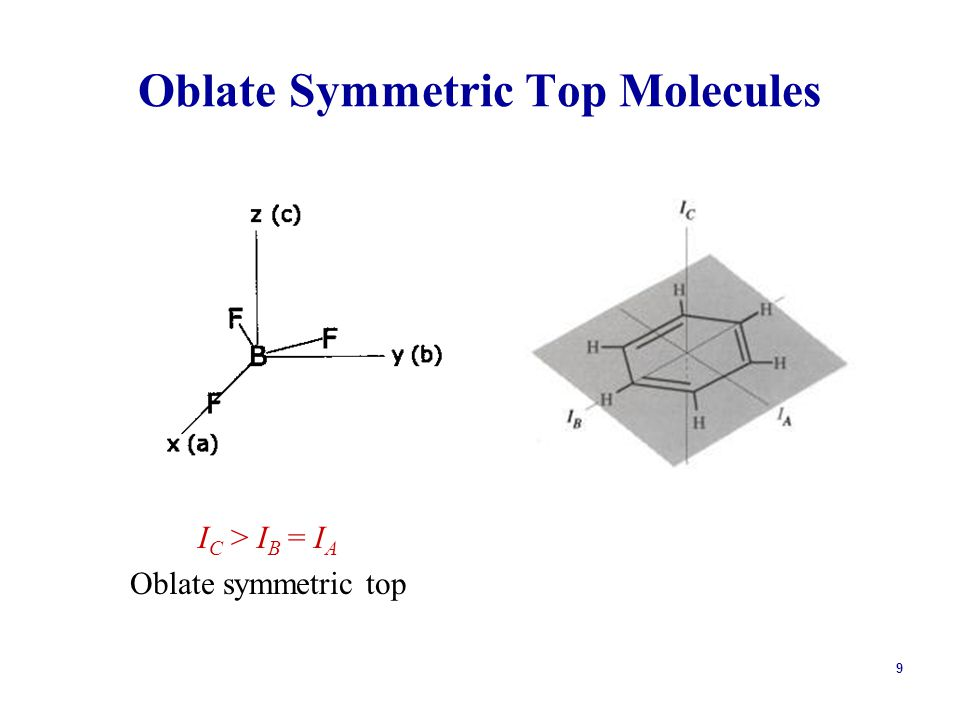
\includegraphics[width=120mm]{Oblate.jpg}
%    \caption{\textbf{Figure O}}
%   \label{fig:label}
%\end{figure}

The potential contribution is also in the \begin{math} \ket{J K M} \end{math} basis. 

\begin{equation} \label{eq:256}
\bra{J K M}\vec{\mu}\cdot\vec{E}\ket{J' K' M'} \hspace{0.125cm} = \hspace{0.125cm} \bra{J K M}\mu E\cos\theta\ket{J' K' M'} \hspace{0.125cm} = \hspace{0.125cm} \mu E\bra{J K M}\cos\theta\ket{J' K' M'} \hspace{0.125cm}.
\end{equation}











\subsubsection{Electronic Structure Calculations}

Electronic Structure Calculations are of high importance in quantum chemistry because a theoretical model of materials aids in the understanding of experimental observations as well as the development of new materials. A good resource for simulating electronic structure is quantum espresso \url{https://www.quantum-espresso.org/} based on density functional theory, plane waves and psuedopotentials. They have pseudopotentials built for all naturally occurring elements. 











\subsubsection{PIMC}

The quantum mechanical partition function is defined as;

\begin{equation} \label{eq:1}
Z \hspace{0.125cm} = \hspace{0.125cm} Tr\hat{\rho} \hspace{0.125cm} .
\end{equation}

The trace operator is a sum over the diagonal elements of the density matrix (which we define as \begin{math} \hat{\rho} \hspace{0.125cm} \equiv \hspace{0.125cm} e^{-\beta \hat{H}} \end{math}), and it can be calculated as an integral in the continuous coordinate basis \begin{math} \ket{q} \end{math};

\begin{equation} \label{eq:1}
Z \hspace{0.125cm} = \hspace{0.125cm} \int dq \bra{q} e^{-\beta \hat{H}} \ket{q} \hspace{0.125cm} .
\end{equation}

The Hamiltonian \begin{math} \hat{H} \end{math} can be represented generally as having a kinetic term \begin{math} \hat{T} \end{math} and a potential term \begin{math} \hat{V} \end{math}, so the previous formulae can be re-expressed as;

\begin{equation} \label{eq:1}
Z  \hspace{0.125cm} = \hspace{0.125cm} \int dq \bra{q} e^{-\beta ( \hat{T} + \hat{V} )}\ket{q} \hspace{0.125cm} , 
\end{equation}

To evaluate the potential and kinetic density matrices separately we need to analyze following statement (splitting the potential part of the Hamiltonian into two half contributions is a convention that will be explained later); 

\begin{equation} \label{eq:1}
e^{-\beta ( \frac{\hat{V}}{2} + \hat{T} + \frac{\hat{V}}{2} )} \hspace{0.125cm} \simeq \hspace{0.125cm} e^{-\beta \frac{\hat{V}}{2}} e^{-\beta \hat{T}} e^{-\beta \frac{\hat{V}}{2}} \hspace{0.125cm} .
\end{equation}

Performing a Taylor series expansion to the RHS here we obtain;

\begin{equation} \label{eq:1}
e^{-\beta \frac{\hat{V}}{2}} e^{-\beta \hat{T}} e^{-\beta \frac{\hat{V}}{2}} \hspace{0.125cm} = \hspace{0.125cm} \Big( 1 - \beta \frac{\hat{V}}{2} + \beta^2 \frac{\hat{V}^2}{8} \Big) \Big( 1 - \beta \hat{T} + \beta^2 \frac{\hat{T}^2}{2} \Big) \Big( 1 - \beta \frac{\hat{V}}{2} + \beta^2 \frac{\hat{V}^2}{8} \Big) \hspace{0.125cm} ,
\end{equation}

and we neglect terms \begin{math} \mathcal{O}(\beta^3) \end{math} or greater because a large \begin{math} T \end{math} means a small \begin{math} \beta \end{math}. For smaller temperature cases we require a mathematical tool known as the Trotter expansion, finishing off this expansion;

\begin{equation} \label{eq:1}
= \hspace{0.125cm} 1 - \beta \Big( \frac{\hat{V}}{2} + \hat{T} + \frac{\hat{V}}{2} \Big) + \frac{\beta^2}{2} \Big( \frac{\hat{V^2}}{4} + \hat{T} + \frac{\hat{V^2}}{4} \Big) +  \frac{\beta^2}{2} \Big( \hat{V} \hat{T} + \hat{T} \hat{V} \Big) \hspace{0.125cm} .
\end{equation}

\begin{equation} \label{eq:1}
e^{-\beta \frac{\hat{V}}{2}} e^{-\beta \hat{T}} e^{-\beta \frac{\hat{V}}{2}} \hspace{0.125cm} = \hspace{0.125cm} e^{-\beta ( \frac{\hat{V}}{2} + \hat{T} + \frac{\hat{V}}{2} )} + \frac{\beta^2}{2} \{ \hat{V} , \hat{T} \}  \hspace{0.125cm} .
\end{equation}

\begin{equation} \label{eq:1}
\therefore  \hspace{0.225cm}  e^{-\beta \frac{\hat{V}}{2}} e^{-\beta \hat{T}} e^{-\beta \frac{\hat{V}}{2}} \hspace{0.125cm} \simeq \hspace{0.125cm} e^{-\beta ( \frac{\hat{V}}{2} + \hat{T} + \frac{\hat{V}}{2} )} \hspace{0.125cm} .
\end{equation}

The Trotter expansion makes this approximation exact. It is defined as;

\begin{equation} \label{eq:1}
e^{-\beta ( \frac{\hat{V}}{2} + \hat{T} + \frac{\hat{V}}{2} )} \hspace{0.125cm} = \hspace{0.125cm} \lim_{P \rightarrow \infty} \bigg[ e^{-\beta \frac{\hat{V}}{2}} e^{-\beta \hat{T}} e^{-\beta \frac{\hat{V}}{2}} \bigg]^P \hspace{0.125cm} .  
\end{equation}

We define \begin{math} \Omega \end{math} such that our maths look less overwhelming;

\begin{equation} \label{eq:1}
\Omega \hspace{0.125cm} = \hspace{0.125cm} e^{-\frac{\hat{\beta V}}{2 P}} e^{- \frac{\hat{\beta T}}{P}} e^{- \frac{\hat{\beta V}}{2 P}} \hspace{0.125cm} , 
\end{equation}

and we use it to redefine our partition function as;

\begin{equation} \label{eq:1}
Z \hspace{0.125cm} = \hspace{0.125cm}  \lim_{P \rightarrow \infty} \int dq \bra{q} \Omega^P \ket{q} \hspace{0.125cm} , 
\end{equation}

We employ the resolution of the identity to this expression after reinterpreting \begin{math} \ket{q} \end{math} as \begin{math} \ket{q_1}\end{math}; 

\begin{equation} \label{eq:1}
\int dq_1 \bra{q_1} \Omega^2 \ket{q_1} \hspace{0.125cm} = \hspace{0.125cm} \int dq_1 \int dq_2 \bra{q_1} \Omega \ket{q_2} \bra{q_2} \Omega \ket{q_1} \hspace{0.125cm} , 
\end{equation}

and obtain the partition function as;

\begin{equation} \label{eq:1}
Z \hspace{0.125cm} = \hspace{0.125cm}  \lim_{P \rightarrow \infty} \int dq_1 \int dq_2 ... \int dq_{P - 1} \int dq_P \Big[ \prod_{i=1}^{P} \bra{q_i} \Omega  \ket{q_{i+1}} \Big]_{q_{P+1} = q_1} \hspace{0.125cm} , 
\end{equation}

We will evaluate the potential and kinetic terms one at a time, starting with trivial potential terms;

\begin{equation} \label{eq:1}
\bra{q_i} e^{-\frac{\beta \hat{V}}{2 P}} \hspace{0.125cm} = \hspace{0.125cm} e^{-\frac{\beta \hat{V}(q_i)}{2 P}} \hspace{0.125cm} , 
\end{equation}

\begin{equation} \label{eq:1}
e^{-\frac{\beta \hat{V}}{2 P}} \ket{q_{i+1}} \hspace{0.125cm} = \hspace{0.125cm} e^{-\frac{\beta \hat{V}(q_{i+1})}{2 P}} \hspace{0.125cm} , 
\end{equation}

So now our expression \begin{math} \bra{q_i} \Omega \ket{q_{i+1}} \end{math} becomes;

\begin{equation} \label{eq:1}
\bra{q_i} \Omega \ket{q_{i+1}} \hspace{0.125cm} = \hspace{0.125cm}  e^{-\frac{\beta \hat{V}(q_i)}{2 P}} \bra{q_i} e^{- \frac{\beta \hat{p}^2}{2 m P}} \ket{q_{i+1}} e^{-\frac{\beta \hat{V}(q_{i+1})}{2 P}}  \hspace{0.125cm} , 
\end{equation}

The kinetic energy term can be evaluated by inserting momentum basis states using the resolution of the identity (i.e. \begin{math} 1 \hspace{0.025cm} = \hspace{0.025cm} \int d^n p \ket{p} \bra{p} \end{math}), but some background is required on the inner product of coordinate and momentum states;

The statement;

\begin{equation} \label{eq:1}
\langle q | p \rangle \hspace{0.125cm} = \hspace{0.125cm} \frac{1}{(2 \pi \hbar)^{\frac{n}{2}}} e^{\frac{i p q}{\hbar}} \hspace{0.125cm} , 
\end{equation}

must be true such that;

\begin{equation} \label{eq:1}
\langle q | q' \rangle \hspace{0.125cm} = \hspace{0.125cm} \int d^n p \langle q | p \rangle \langle p | q' \rangle \hspace{0.125cm} = \hspace{0.125cm} \delta ( x - x' )  \hspace{0.125cm} , 
\end{equation}

remains valid. Note \begin{math} \langle p | q' \rangle  \hspace{0.025cm} = \hspace{0.025cm} \langle q' | p \rangle^{*} \hspace{0.025cm} = \hspace{0.025cm} \frac{1}{(2 \pi \hbar)^{\frac{n}{2}}} e^{\frac{- i p q'}{\hbar}}  \end{math}, so our above expression becomes;

\begin{equation} \label{eq:1}
\langle q | q' \rangle \hspace{0.125cm} = \hspace{0.125cm} \frac{1}{(2 \pi \hbar)^{n}} \int d^n p \hspace{0.05cm} e^{\frac{i p (q - q')}{\hbar}} \hspace{0.125cm} \equiv \hspace{0.125cm} \delta ( x - x' ) \hspace{0.125cm} .
\end{equation}

Now, continuing with the process of solving \begin{math} \bra{q_i} e^{ - \frac{ \beta p^2}{2 m P}} \ket{q_{i+1}} \end{math}; 

\begin{equation} \label{eq:1}
\bra{q_i} e^{ - \frac{ \beta p^2}{2 m P}} \ket{q_{i+1}} \hspace{0.125cm} = \hspace{0.125cm} \int d^n p \hspace{0.05cm} \bra{q_i} e^{ - \frac{ \beta \hat{p}^2}{2 m P}} \ket{p} \langle p | q_{i+1} \rangle \hspace{0.125cm} .
\end{equation}

Note that;

\begin{equation} \label{eq:1}
\bra{q} e^{ - \frac{ \beta \hat{p}^2}{2 m P}} \ket{p} \hspace{0.025cm} = \hspace{0.025cm} \bra{q} e^{ - \frac{ \beta p^2}{2 m P}} \ket{p} \hspace{0.025cm} = \hspace{0.025cm} \langle q | p \rangle e^{ - \frac{ \beta p^2}{2 m P}} \hspace{0.025cm} ,
\end{equation}

\begin{equation} \label{eq:1}
\bra{q_i} e^{ - \frac{ \beta p^2}{2 m P}} \ket{q_{i+1}} \hspace{0.125cm} = \hspace{0.125cm} \frac{1}{(2 \pi \hbar)^{n}} \int d^n p \hspace{0.05cm} \exp\Big({ - \frac{ \beta \hat{p}^2}{2 m P}}\Big)  \exp\Big({\frac{i p (q_i - q_{i+1})}{\hbar}}\Big)  \hspace{0.125cm} .
\end{equation}

Note that this has the form of a Gaussian integral, which has the solution; 

\begin{equation} \label{eq:1}
\int_{- \infty}^{\infty} \exp\Big({ -a p^2 + b p}\Big) dp \hspace{0.125cm} = \hspace{0.125cm} \sqrt{\frac{\pi}{a}} \exp\Big({\frac{b^2}{4 a}}\Big) \hspace{0.125cm} .
\end{equation}

Noting that in this scenario, \begin{math} a \hspace{0.025cm} = \hspace{0.025cm} \frac{\beta}{2 m P} \end{math} and \begin{math} b \hspace{0.025cm} = \hspace{0.025cm} \frac{i (q_i - q_{i + 1})}{\hbar} \end{math}, so;

\begin{equation} \label{eq:1}
\bra{q_i} e^{ - \frac{ \beta p^2}{2 m P}} \ket{q_{i+1}} \hspace{0.125cm} = \hspace{0.125cm} \frac{1}{(2 \pi \hbar)} \sqrt{\frac{2 \pi m P}{\beta}} \exp{\Big( \frac{ - m P (q_i - q_{i+1})^2}{2 \hbar^2 \beta}\Big)}  \hspace{0.125cm} .
\end{equation}

\begin{equation} \label{eq:1}
\bra{q_i} e^{ - \frac{ \beta p^2}{2 m P}} \ket{q_{i+1}} \hspace{0.125cm} = \hspace{0.125cm} \sqrt{\frac{m P}{2 \pi \hbar^2 \beta}} \exp{\Big( \frac{ - m P (q_i - q_{i+1})^2}{2 \hbar^2 \beta}\Big)} \hspace{0.125cm} .
\end{equation}

If we state that \begin{math} \kappa \hspace{0.025cm} = \hspace{0.025cm} \frac{m P}{2 \pi \hbar^2 \beta} \end{math} (note \begin{math} \kappa \hspace{0.025cm} \equiv \hspace{0.025cm} \Big[ \frac{kg \cdot \frac{kg m^2}{s^2}}{\frac{kg^2 m^4}{s^4} \cdot s^2}  \Big] \hspace{0.025cm} \equiv \hspace{0.025cm} \Big[ \frac{1}{m^2} \Big]  \end{math} ), then the above expression becomes;

\begin{equation} \label{eq:1}
\bra{q_i} e^{ - \frac{ \beta p^2}{2 m P}} \ket{q_{i+1}} \hspace{0.125cm} = \hspace{0.125cm} \sqrt{\frac{\kappa}{\pi}} \exp{\Big( - \kappa (q_i - q_{i+1})^2 \Big)} \hspace{0.125cm} .
\end{equation}

Using this result we can write Z as;

\begin{equation} \label{eq:1}
Z \hspace{0.125cm} = \hspace{0.125cm} \lim_{P \rightarrow \infty} \Bigg[ \bigg(\sqrt{\frac{m P}{2 \pi \hbar^2 \beta}}\bigg)^{P} \bigg[ \prod_{i=1}^{P} \int d q_i \bigg] \exp{- \bigg( \sum_{i = 1}^{P} \bigg[ \frac{ m P (q_i - q_{i+1})^2}{2 \hbar^2 \beta} + \frac{\beta}{2P} \Big( V(q_i) + V(q_{i + 1}) \Big) \bigg] \bigg)} \Bigg]_{q_{P + 1} \hspace{0.05cm} = \hspace{0.05cm} q_1} \hspace{0.125cm} .
\end{equation}

Noting that \begin{math} V(q_i) \end{math} is always counted twice in the sum \begin{math} \sum_{i = 1}^{P} \Big( V(q_i) + V(q_{i + 1}) \Big) \end{math} because \begin{math} V(q_1) \hspace{0.025cm} = \hspace{0.025cm} V(q_{i + 1}) \end{math}, we can rewrite the partition function as; 

\begin{equation} \label{eq:1}
Z \hspace{0.125cm} = \hspace{0.125cm} \lim_{P \rightarrow \infty} \Bigg[ \bigg(\sqrt{\frac{m P}{2 \pi \hbar^2 \beta}}\bigg)^{P} \bigg[ \prod_{i=1}^{P} \int d q_i \bigg] \exp{- \bigg( \sum_{i = 1}^{P} \Big[ \frac{ m P (q_i - q_{i+1})^2}{2 \hbar^2 \beta} + \frac{\beta}{P} V(q_i) \Big] \bigg)} \Bigg]_{q_{P + 1} \hspace{0.05cm} = \hspace{0.05cm} q_1} \hspace{0.125cm} .
\end{equation}

\subsubsubsection{Internal Energy for PIMC}

The internal energy is traditionally calculated as;

\begin{equation} \label{eq:1}
U \hspace{0.125cm} = \hspace{0.125cm} \sum_{i = 1}^{\infty} g_i p_i \epsilon_{i} \hspace{0.125cm} ,
\end{equation}

where \begin{math} p_i \end{math}, the probability of a particle being in a given quantum state \begin{math} \epsilon_{i} \end{math}, is given by;

\begin{equation} \label{eq:1}
p_i \hspace{0.125cm} = \hspace{0.125cm} \frac{\exp \big(\frac{- \epsilon_i}{k_B T}\big)}{Z}  \hspace{0.125cm} ,
\end{equation}

The partition function in its most basic form has the expression;

\begin{equation} \label{eq:1}
Z \hspace{0.125cm} = \hspace{0.125cm} \sum_{i = 1}^{\infty} g_i \exp \Big(\frac{- \epsilon_i}{k_B T}\Big) \hspace{0.125cm} ,
\end{equation}

where \begin{math} \beta \hspace{0.025cm} = \hspace{0.025cm} \frac{1}{k_B T} \end{math} There is a relationship between the internal energy and this most basic form of the partition function;

\begin{equation} \label{eq:1}
U \hspace{0.125cm} = \hspace{0.125cm} \sum_{i = 1}^{\infty} \frac{g_i \epsilon_{i} \exp \big(- \beta \epsilon_i \big)}{Z} \hspace{0.125cm} = \hspace{0.125cm} - \frac{\partial}{\partial{\beta}}\sum_{i = 1}^{\infty} \frac{g_i \exp \big(- \beta \epsilon_i \big)}{Z} \hspace{0.125cm} = \hspace{0.125cm} - \frac{1}{Z} \frac{\partial Z}{\partial{\beta}}   \hspace{0.125cm} .
\end{equation}

With some added maths it can be shown that;

\begin{equation} \label{eq:1}
- \frac{\partial{\ln{Z}}}{\partial{Z}} \hspace{0.125cm} = \hspace{0.125cm} - \frac{1}{Z} \hspace{0.125cm} \rightarrow \hspace{0.125cm} - \partial{\ln{Z}} \hspace{0.125cm} = \hspace{0.125cm} - \frac{\partial{Z}}{Z} \hspace{0.125cm}, 
\end{equation}

so;

\begin{equation} \label{eq:1}
U \hspace{0.125cm} = \hspace{0.125cm} - \frac{1}{Z} \frac{\partial{Z}}{\partial{\beta}} \hspace{0.125cm} = \hspace{0.125cm} - \frac{\partial \ln{Z}}{\partial{\beta}} \hspace{0.125cm} .
\end{equation}

To make it look possibly prettier we do some more maths to show;

\begin{equation} \label{eq:1}
\frac{\partial{\beta}}{\partial{T}} \hspace{0.125cm} = \hspace{0.125cm} - \frac{1}{k_B T^2} \hspace{0.125cm} \rightarrow \hspace{0.125cm} - \partial{\beta} \hspace{0.125cm} = \hspace{0.125cm} - \frac{\partial{T}}{k_B T^2} \hspace{0.125cm} \rightarrow \hspace{0.125cm} - \frac{1}{\partial{\beta}} \hspace{0.125cm} = \hspace{0.125cm} - \frac{k_B T^2}{\partial{T}} \hspace{0.125cm} , 
\end{equation}

so 

\begin{equation} \label{eq:1}
U \hspace{0.125cm} = \hspace{0.125cm} - \frac{1}{Z} \frac{\partial{Z}}{\partial{\beta}} \hspace{0.125cm} = \hspace{0.125cm} k_B T^2 \frac{\partial{\ln{Z}}}{\partial{T}} \hspace{0.125cm} ,
\end{equation}

however we will build off of our previous result ( \begin{math} U \hspace{0.125cm} = \hspace{0.125cm} - \frac{\partial \ln{Z}}{\partial{\beta}} \end{math} ) instead.

Logically, we should now go the density matrix representation of internal energy that is used in PIMC. The density matrices for the system (generally speaking) depend on a partitioned product of density matrices for simpler systems, which if treated as independant are more easily solvable (this is directly analogous to the partition function being constructed from smaller partition functions \begin{math} Z \hspace{0.025cm} = \hspace{0.025cm} Z_{trans} Z_{vib} Z_{rot} Z_{electronic} \end{math}). If we define \begin{math} \vec{R} \hspace{0.025cm} = \hspace{0.025cm} (\vec{r};\vec{\Omega})  \hspace{0.025cm} = \hspace{0.025cm} (x,y,z;\phi,\theta,\chi) \end{math}, then the density matrix can be shown generally as;

\begin{equation} \label{eq:1}
\hat{\rho} \hspace{0.125cm} = \hspace{0.125cm} \bra{\vec{R}} \exp \big( - \beta \hat{H} \big) \ket{\vec{R}} \hspace{0.025cm} , 
\end{equation}

where the Hamiltonian for quantum systems is typically defined as having translational, vibrational, rotational, and electronic components;

\begin{equation} \label{eq:1}
\hat{H} \hspace{0.125cm} = \hspace{0.125cm} \hat{T}_{trans} + \hat{H}_{vib} + \hat{T}_{rot} + \hat{V}_{pot} \hspace{0.025cm} .
\end{equation}

Neglecting \begin{math} \hat{H}_{vib} \end{math} for now, keeping our solution for \begin{math} \hat{V}_{pot} \end{math} as it is valid, and reminding ourselves that we already found a valid PIMC solution for the transitional density matrix because \begin{math} \hat{T}_{trans} \hspace{0.025cm} = \hspace{0.025cm} \frac{\hat{p}^2}{2 m} \end{math}, we represent the density matrix as;

\begin{equation} \label{eq:1}
\hat{\rho} \hspace{0.125cm} = \hspace{0.125cm} \bra{\vec{R}} \exp \big( - \beta \big( \frac{\hat{V}_{pot}}{2} + \hat{T}_{trans} + \hat{T}_{rot} + \frac{\hat{V}_{pot}}{2} \big) \big) \ket{\vec{R}} \hspace{0.025cm} . 
\end{equation}

We use the assumption that temperature is very large so we can separate the Hamiltonians (we'll incorporate the Trotter expansion to make this valid for all non-zero temperatures) into their own exponentionals. 

\begin{equation} \label{eq:1}
\hat{\rho} \hspace{0.125cm} \simeq \hspace{0.125cm} \bra{\vec{R}} \exp \Big( - \frac{ \beta \hat{V}_{pot}}{2} \Big) \exp \Big( - \frac{\beta \hat{p}^2}{2 m} \Big)  + \exp \Big( - \beta \hat{T}_{rot} \Big) \exp \Big( - \frac{ \beta \hat{V}_{pot}}{2} \Big)  \ket{\vec{R}} \hspace{0.025cm} . \end{equation}

Its useful to note that even though we made this approximation, the bra's and kets still operate on each exponential individually much like how they would have if expanded the original representation as a taylor series. I will do a quick aside to show this. We assume that;

\begin{equation} \label{eq:1}
\beta \big( \frac{\hat{V}_{pot}}{2} + \hat{T}_{trans} + \hat{T}_{rot} + \frac{\hat{V}_{pot}}{2} \big)  \hspace{0.125cm} \gg \hspace{0.125cm} \frac{\beta^2}{2} \big( \frac{\hat{V}_{pot}}{2} + \hat{T}_{trans} + \hat{T}_{rot} + \frac{\hat{V}_{pot}}{2} \big)^2 \hspace{0.125cm} ,
\end{equation}

and so it is a valid assumption (that i'm only doing to make the demonstration of this proof easier) to state that

\begin{equation} \label{eq:1}
\exp \big( - \beta \big( \frac{\hat{V}_{pot}}{2} + \hat{T}_{trans} + \hat{T}_{rot} + \frac{\hat{V}_{pot}}{2} \big) \big) \hspace{0.125cm} \simeq \hspace{0.075cm} 1 \hspace{0.075cm} - \hspace{0.125cm} \beta \big( \frac{\hat{V}_{pot}}{2} + \hat{T}_{trans} + \hat{T}_{rot} + \frac{\hat{V}_{pot}}{2} \big) \hspace{0.125cm} ,
\end{equation}

and operating on the ket, then having the bra operate on the resulting term we obtain;

\begin{equation} \label{eq:1}
\hat{\rho} \hspace{0.125cm} \simeq \hspace{0.125cm} \bra{\vec{R}} \bigg[ 1 \hspace{0.075cm} - \hspace{0.125cm} \beta \big( \frac{\hat{V}_{pot}}{2} + \hat{T}_{trans} + \hat{T}_{rot} + \frac{\hat{V}_{pot}}{2} \big) \hspace{0.125cm} \bigg] \ket{\vec{R}} \hspace{0.125cm} ,
\end{equation}

and these operators have some result for their eigenvalues (and the potentials are the same for the same \begin{math} \vec{R} \end{math};

\begin{equation} \label{eq:1}
\hat{\rho} \hspace{0.125cm} \simeq \hspace{0.125cm} \bra{\vec{R}} \bigg[ 1 \hspace{0.075cm} - \hspace{0.125cm} \beta \big( E_{trans} + E_{rot} + V(\vec{R})\big) \hspace{0.125cm} \bigg] \ket{\vec{R}} \hspace{0.125cm} ,
\end{equation}

which can be re-represented exactly in an exponential form as;

\begin{equation} \label{eq:1}
\hat{\rho} \hspace{0.125cm} = \hspace{0.125cm} \bra{\vec{R}} \exp \Big( - \beta \big( E_{trans} + E_{rot} + V(\vec{R})\big) \Big) \ket{\vec{R}} \hspace{0.125cm} .
\end{equation}

The main point is that the bras and kets act on each of these Hamiltonian operators individually to create independent energy eigenvalues by assuming they combination of Hamiltonians form a set of independent linear differential equations. Going back to our original representation with the Hamiltonian operators;

\begin{equation} \label{eq:1}
\hat{\rho} \hspace{0.125cm} \simeq \hspace{0.125cm} \bra{\vec{R}} \exp \Big( - \frac{\beta \hat{p}^2}{2 m} \Big) \exp \Big( - \beta \hat{T}_{rot} \Big) \exp \Big( - \beta \hat{V}_{pot} \Big)  \ket{\vec{R}} \hspace{0.025cm} . \end{equation}

The bra and ket act differently on the translational, rotational, and potential terms in each case. The tranlational terms are independant of the Euler Angles \begin{math} \vec{\Omega} \end{math}, and the rotational terms are independant of Cartesian Coordinates \begin{math} \vec{r} \end{math}, so we will express their density matrices as having only the components of the bra and ket that act upon them, and the potential density matrix will have the full set of basis coordinates \begin{math} \vec{R} \end{math}. The previous term can also be represented as;

\begin{equation} \label{eq:1}
\hat{\rho} \hspace{0.125cm} \simeq \hspace{0.125cm} \bra{\vec{r}} \exp \Big( - \frac{\beta \hat{p}^2}{2 m} \Big) \ket{\vec{r}} \bra{\vec{\Omega}} \exp \Big( - \beta \hat{T}_{rot} \Big) \ket{\vec{\Omega}} \bra{\vec{R}} \exp \Big( - \beta \hat{V}_{pot} \Big) \ket{\vec{R}} \hspace{0.025cm} . \end{equation}

Taking this into a more compact form we have;

\begin{equation} \label{eq:1}
\hat{\rho} \hspace{0.125cm} \simeq \hspace{0.125cm} \hat{\rho}_{trans} \hat{\rho}_{rot} \hat{\rho}_{pot} \hspace{0.025cm} .
\end{equation}

Where is should be clear that;

\begin{equation} \label{eq:1}
\hat{\rho}_{trans} \hspace{0.125cm} = \hspace{0.125cm} \bra{\vec{r}} \exp \Big( - \frac{\beta \hat{p}^2}{2 m} \Big) \ket{\vec{r}} \hspace{0.025cm} 
\end{equation}

\begin{equation} \label{eq:1}
\hat{\rho}_{rot} \hspace{0.125cm} = \hspace{0.125cm} \bra{\vec{\Omega}} \exp \Big( - \beta \hat{T}_{rot} \Big) \ket{\vec{\Omega}} \hspace{0.025cm} 
\end{equation}

\begin{equation} \label{eq:1}
\hat{\rho}_{pot} \hspace{0.125cm} = \hspace{0.125cm} \bra{\vec{R}} \exp \Big( - \beta \hat{V}_{pot} \Big) \ket{\vec{R}} \hspace{0.025cm} .
\end{equation}

Going back to the partition function;

\begin{equation} \label{eq:1}
Z \hspace{0.125cm} = \hspace{0.125cm} Tr\hat{\rho} \hspace{0.125cm} .
\end{equation}

This time working with the \begin{math} (x, y, z, \phi, \theta, \chi) \end{math} Cartesian and Euler Angle basis vectors, we have the continuous representation of;

\begin{equation} \label{eq:1}
Z \hspace{0.125cm} = \hspace{0.125cm} \int d \vec{R} \bra{\vec{R}} \rho \ket{\vec{R}} \hspace{0.125cm} .
\end{equation}

Performing the Trotter expansion we can re-express our old result as;

\begin{equation} \label{eq:1}
Z \hspace{0.125cm} = \hspace{0.125cm}  \lim_{P \rightarrow \infty} \int d \vec{R}_1 \int d \vec{R}_2 ... \int d \vec{R}_{P - 1} \int d \vec{R}_P \Big[ \prod_{i=1}^{P} \bra{\vec{R}_i} \Omega \ket{\vec{R}_{i+1}} \Big]_{\vec{R}_{P+1} = \vec{R}_1} \hspace{0.125cm} , 
\end{equation}

Now notation is important. We say that;

\begin{equation} \label{eq:1}
\hat{\rho}_i \hspace{0.125cm} = \hspace{0.125cm} \bra{\vec{R}_i} \Omega \ket{\vec{R}_{i+1}} \hspace{0.125cm} , 
\end{equation}

and additionally that;

\begin{equation} \label{eq:1}
\hat{\rho}_i \hspace{0.125cm} = \hspace{0.125cm} \hat{\rho}_{trans_i} \hat{\rho}_{rot_i} \hat{\rho}_{pot_i} \hspace{0.125cm} .
\end{equation}

We define tau as \begin{math} \tau \hspace{0.025cm} = \hspace{0.025cm} \frac{\beta}{P} \end{math}, and remind ourselves that;

\begin{equation} \label{eq:1}
\hat{\rho} \hspace{0.125cm} = \hspace{0.125cm} \bra{\vec{R}_i} \exp \Big( - \frac{\beta}{P} \big( \hat{T}_{trans} + \hat{T}_{rot} + \hat{V}_{pot} \big) \Big) \ket{\vec{R}_{i+1}}
\end{equation}

\begin{equation} \label{eq:1}
\hat{\rho} \hspace{0.125cm} = \hspace{0.125cm} \bra{\vec{R}_i} \exp \Big( - \tau \big( \hat{T}_{trans} + \hat{T}_{rot} + \hat{V}_{pot} \big) \Big) \ket{\vec{R}_{i+1}}
\end{equation}

\begin{equation} \label{eq:1}
\hat{\rho} \hspace{0.125cm} = \hspace{0.125cm} \bra{\vec{R}_i} \exp \Big( - \tau \big( E_{trans} + E_{rot} + V(\vec{R})\big) \Big) \ket{\vec{R}_{i+1}} \hspace{0.125cm} .
\end{equation}

Much like how \begin{math} U \hspace{0.025cm} = \hspace{0.025cm} - \frac{\partial{\ln{Z}}}{\partial{\beta}} \end{math}, a similar expression is true for \begin{math} \tau \end{math} when trying to find the partial energy contributions from \begin{math} \hat{\rho}_{trans_i} \end{math}, \begin{math} \hat{\rho}_{rot_i} \end{math} and \begin{math} \hat{\rho}_{pot_i} \end{math}. We name these energies \begin{math} \epsilon_{trans_i} \end{math}, \begin{math} \epsilon_{rot_i} \end{math}, and \begin{math} \epsilon_{pot_i} \end{math}, respectively;

\begin{equation} \label{eq:1}
\epsilon_{trans_i} \hspace{0.125cm} = \hspace{0.125cm} - \frac{\partial{\ln{\hat{\rho}_{trans_i}}}}{\partial{\tau}}
\end{equation}

\begin{equation} \label{eq:1}
\epsilon_{rot_i} \hspace{0.125cm} = \hspace{0.125cm} - \frac{\partial{\ln{\hat{\rho}_{rot_i}}}}{\partial{\tau}}
\end{equation}

\begin{equation} \label{eq:1}
\epsilon_{trans_i} \hspace{0.125cm} = \hspace{0.125cm} - \frac{\partial{\ln{\hat{\rho}_{pot_i}}}}{\partial{\tau}}\hspace{0.125cm} .
\end{equation}


\subsection{Solid State Physics}

\subsubsection{Drude Theory of Electron's in Solids}

The Drude theory was the first model for electron collisions and conductivity, and was based around kinetic theory for gases and has some key assumptions. Firstly there is some mean collision time \begin{math} \tau \end{math}. Secondly, \begin{math} \vec{p} \hspace{0.125cm} = \hspace{0.125cm} \vec{0} \end{math} following a collision. Lastly, electrons act as free electrons with their motion determined by electric magnetic fields (i.e. \begin{math} \vec{F} \hspace{0.125cm} = \hspace{0.125cm} q ( \vec{E} + \vec{v} \times \vec{B} ) \end{math} ) . 

\subsection{Relativity}

\begin{equation} \label{eq:101}
t \hspace{0.125cm} = \hspace{0.125cm} \frac{t_0}{\big(1 - \frac{v^{2}}{c^{2}} \big)^\frac{1}{2}}
\end{equation}

\subsection{Theory of Everything}
\subsubsection{Standard Model}
The standard model is modern humanities best T.O.E model of observable universe. Not to be confused with the unobservable universe, the um? 97 \% of the universe that is dark matter and dark energy we can?t actually observe. None the less, it explains close to the entirety of the phenomenon we are confident we?ve observed since the dawn of recording observations. \\


\textit{Motivation}

I want to go over my current perspective on the standard model using the most amount of math I can quickly and confidently explain to someone who kind of knows what im talking about and is willing to periodically rewind the video to hear my? explanations.  I want to explain some basic physical concepts that I might build on in later videos in order to illustrate my perspective on various.. things. This is my one motivator to make this, and the second is that I want to display the modern execution of the scientific method, our search for answers to fundamental questions, and the limits that fundamentally hold us back from those answers. \\

\textit{Natures like weird elementary particle KNEX}

The standard model consists of 16 elementary particles some of which are mass, charge and or colour* containing half integer spin Fermions and some of which interact via integer spin Bosons that all travel at light speed, and one of which is the Higgs Boson (a.k.a the God Particles) which through creates mass through a intricate and elegant process called read the fucking manga? you weeeeb. The particles path through time are governed by the equation of motion derived from their Lagrangian and their initial positions and velocities, and their Lagrangian is the differential equation representation of the system overall kinetic and potential energy. The most common observed interactions are the formation of proton and neutrons from quarks, the subsequent interaction between the protons and neutrons, and the even more subsequent interaction of electrons with already bonded protons and neutrons forming all the atoms of the periodic table? following a few sun?s exploding that is. These building blocks make up all of chemistry and to have an in depth understanding of the laws of chemistry involved understanding quantum mechanics and electromagnetism and statistical thermodynamics. To understand biology or inorganic chemistry or polymer science thoroughly you must understand biochemistry, solid state physics, and organic chemistry and conveniently to understand biochemistry that thoroughly you must have to understand organic chemistry. This builds all the way up but it breaks down to a few simple rules; things tend to increasing complexity (or information), and things tend to decreasing energy (or more relaxed in energy level), and things interact to do both of these things. \\
\\

\textit{Lagrangian Stuff}

To thoroughly explain Lagrangian mechanics would take a while, but the jist of it is that you have a Lagrangian which is a differential equation representation of the systems energy, and you want to minimize something called the action which is the value of the integral of the Lagrangian within some arbitrary time interval. The result of this minimization is another differential equation derived from the Euler Lagrange equation which computes the systems equation of motion using partial derivatives of the Lagrangian. Long story short we input a Lagrangian, and output some differential equation(s) (possibly coupled partial differential equations) that?s luckily probably already been solved 100 years ago so we can get straight up get the equation of motion for this systems Lagrangian. When you have all the equations of motion for all the elementary particles in the universe then you can predict the future? well to bad you can?t (lol Uncertainty Principle? not getting into why not this video is long enough). This still doesn?t seem to explain everything though. \\

\textit{Enter Statistical Thermodynamics and QED}
  
\section{Chemistry}

%%%%%%%%%%%%%%%%%%%%%%%%%%%%%%%%%%%%%%%%%%%%%%%%
%%%%%%%% BEGINNING OF BIOLOGY SECTION %%%%%%%%%%

\section{Biology}
\subsection{Cell Biology}
\subsubsection{Cell Types}

    There exist many different types of cell throughout the many organs of the human body.
    
    Tissues are a groups of cells with a similar structure and function, and there are 4 common tissues found throughout the human body; epithelial, connective, muscular, and nervous tissue. 

\subsubsubsection{Epithelial Tissue}
\subsubsubsection{Connective Tissue}
\subsubsubsection{Muscular Tissue}
\subsubsubsection{Nervous Tissue}

\subsection{Human Body}
\subsubsection{NeuroEndocrine System}

\textit{Neuroendocrine System}

\textbf{Dopamine}

Its name was derived from the IUPAC chemical name dihydroxyphenethylamine synthesized by removing a carboxyl group from its precursor L-DOPA, which is made from the biosynthesis of the amino acid L-tyrosine. L-DOPA is synthesized in the brain and kidneys, and it is the precursor to other useful biochemicals such as epinephrine and norepinephrine, and these (along with dopamine) are part of a class of chemicals known as catecholamines. It synthesized in plants and most animals. 

Its a neurotransmitter that has several distinct dopamine pathways, one of which plays a major role in the motivation components of reward-motivated behaviour. Because of this, certain drugs which increase dopamine neuronal activity in brain are considered addictive. Dopamine pathways are also involved in motor control and controlling the release of various hormones, so it could possibly be said that compounds that release dopamine (addictive compounds) are physically addictive. 

Dopamine pathways (groups of cells) form a dopamine system which is neuromodulatory. Neuromodulation is a physiological process by which a neutron uses one or more chemicals to regulate a diverse population of neurons. Neuromodulators are neurotransmitters that diffuse through neural tissue to affect low-acting receptors of many neurons. Other examples of neuromodulators include serotonin, acetylcholine, histamine, norepinephrine. They?re known to have modulatory effects on target areas such as decorrelation of spiking, increase of firing rate, sharpening of spatial tuning curves, and maintenance of increased spiking during working memory.



%%%%%%%%%%%%%%%%%%%%%%%%%%%%%%%%%%%%%%%%%%%%%%%%
%%%%%%% BEGINNING OF ECONOMICS SECTION %%%%%%%%%

\section{Economics}
\subsection{Macroeconomics}
\subsection{Microeconomics}

%%%%%%%%%%%%%%%%%%%%%%%%%%%%%%%%%%%%%%%%%%%%%%%%
%%%%%% BEGINNING OF COMPUTATION SECTION %%%%%%%%

\section{Computation}

Main Philosophy: Using computers proficiently is simply a matter of having a coders mindset and knowing how to find out how to do something. That is why this extensive list has been created so that I don?t have to remember a bunch of different commands n stuff.

\subsection{Fundamentals of Computation}

CPU --> Does computations at the scalar level \\
GPU --> Does computations at the vector level \\
MPU --> Does computations at the tensor level \\

\subsubsection{CPU's}

Languages Included: LINUX, python, c++, fortran.

\subsubsection{Useful Wikipedia Articles to Read}

\textbf{Unix Philosophy}

Gives a description of the philosophies that went into designing Unix, and how those philosophies influenced the coding world in general. 



%%%%%%%%%%%%%%%%%%%%
%%%%%% LINUX %%%%%%%
%%%%%%%%%%%%%%%%%%%%

\subsection{LINUX}

\textbf {Basic Commands}

LINUX is a bit different from a language (I think its considered an os (operating system)), but it has its set of useful things to know in order to do stuff like any other coding language like;

\begin{center}
\begin{tabular*}{\textwidth}{ | p{0.262\textwidth} | p{0.664\textwidth}| }
\hline
 \textbf{ssh servername} & cryptographic network protocol for operating network services securely over an unsecured network. I started out with nlogn, BASICALLY ALLOWS ACCESS TO A SERVER\\ 
\hline 
 \textbf{ls} & lists all files and subdirectories in the current directory (directory is a fancy asshole talk for folder) \\  
\hline 
\textbf{ls -a} & lists dot files as well \\   
cd pathname & stands for change directory, will take you to the directory you specify, if you want you can access directories in other directories but extending the path \\
\hline
\textbf{cd} & if no directory is specified the cd command will simply take you back to your earliest directory. \\ 
\hline 
\textbf{cd ..} & will take you one directory back, and if your at the earliest directory it will take you to the home directory. \\ 
\hline 
\end{tabular*}
\end{center}

These commands are enough to give you access to anyone files in a server you have access to; to read and/or edit files you can use vim, emacs, or any other LINUX text editor which have their own set of useful commands. \\

\textit{To edit a file type;} 

vim (or emacs) filename,
and the screen will change and display the information in the file you requested to edit. (see subsection on VIM) \\

\textbf{Additional Commands}

What we have gone through is the basic LINUX/VIM commands. When I use the word basic LINUX commands or basic VIM commands, what I really mean is that understanding these commands is of the utmost importance as they will significantly speed up the process of writing code and troubleshooting. It shouldn?t take too long for a newcomer to get used to using these, especially because they are used so frequently. What I lay out now are things that will be used less frequently...

\begin{center}
\begin{tabular*}{\textwidth}{ | p{0.262\textwidth} | p{0.664\textwidth}| }
\hline
\textbf{sbatch filename} & submits things to the queue \\
\hline 
\textbf{squeue or qstat} & lets you see files in the queue \\
\hline 
\textbf{vimdiff} & compares vim scripts and outputs differences \\
\hline 
\textbf{head filename} & displays the first 10 lines of that file \\ 
\hline 
\textbf{tail filename} & displays the last 10 lines of that file \\ 
\hline 
\textbf{git clone} & copies someones set of code on githib \\ 
\hline 
\textbf{quota -s} & shows the amount of allowed space, and the amount of space taken up \\ 
\hline
\textbf{rm filename} & removes file named filename. \\ 
\hline
\textbf{rm -r directoryname} & removes directory named directoryname and all of its contents so long as there are no write protected file \\ 
\hline
\textbf{rm -rf directoryname} & removes directory named directoryname and force removes any write protected files (I would recommend using this instead of rm -r in almost all cases). \\ 
\hline 
\textbf{grep -r keyword .} & The grep command is used to search text (in this example is searches for the word keyword). It searches the given file for lines containing a match to the given strings or words. It is one of the most useful commands on Linux and Unix-like system. Let us see how to use grep on a Linux or Unix like system. The -r ensures that it searches through all files in a directory and the . symbol specifies that you want to search through the directory you are in. \\ 
\hline 
\end{tabular*}
\end{center}

You can also copy (cp) and move (mv) directories using -r as an additional argument;

\begin{center}
\begin{tabular*}{\textwidth}{ | p{0.262\textwidth} | p{0.664\textwidth}| }
\hline
\textbf{cp -r directoryname} & copies directory and the entirety of the directories contents, and like the original copy command, it requires a path and there is the option of renaming the directory upon pasting it in its new path in the directory. \\
\hline 
\textbf{mv -r directoryname} & moves directory and the entirety of the directories contents, and like the original copy command, it requires a path and there is the option of renaming the directory upon pasting it in its new path in the directory. \\
\hline 
\end{tabular*}
\end{center}

%%%%%%%%%%%%%%%%%%%%%%%%%%%%%%%%%%%%%%%%%%%%%%%%%%%%%%%%%%%%
%%%%%%%%%%%%%%%%%%%%%%%%%%%%%%%%%%%%%%%%%%%%%%%%%%%%%%%%%%%%

%%%%%%%%%%%%%%%%%
%%%%%% VIM %%%%%%
%%%%%%%%%%%%%%%%%

\subsubsection{VIM}

\begin{center}
\begin{tabular*}{\textwidth}{ | p{0.262\textwidth} | p{0.664\textwidth}| }
\hline
\textbf{i} & insert mode: this command allows you to type words while inside of a folder (i.e. edit). note: if you copy text from somewhere using ?c, ?v can be used to paste that specific thing, however you can store something different in your ?copy? space by using visual mode (v). \\ 
\hline 
\textbf{v} & visual mode: lets you copy and paste more accurately. the copy you perform here will be different from the copy you perform with ?c. when you want to copy in visual mode you can highlight the desired text and cut using d, copy using y (yank), and paste using p. \\ 
\hline
\textbf{/} & essentially the command f of vim \\ 
\hline 
\textbf{:vsplit filename} & :vsplit command can be used to look at two documents simultaneously, however you may only navigate through and/or edit one file at a time. to navigate to different screens you can use shift W(h, j, k, l) to navigate up, down, left and right. \\
\hline 
\textbf{:number} & sends you to the line (number) \\ 
\hline 
\textbf{:wq or shift ZZ} & quits with saving \\ 
\hline 
\textbf{:q!} & quits without saving \\
\hline
\textbf{:\%s/oldone/newone} & replaces any segments of text that say oldone with text that says newone \\
\hline
\end{tabular*}
\end{center}

Finally, to run code you need to know how to start it. My alias is currently pydev for interpreted python scripts, and its \texttt{/PATH/\_\_filename\_\_ for c or fortran code (./\_\_filename\_\_ if you are already in the directory which possesses \_\_filename\_\_).} To run to \texttt{\_\_filename\_\_ script, type;
alias \_\_filename\_\_} ,
and depending on the file there may or may not be arguments needed as inputs;
alias \texttt{\_\_filename\_\_ argv[1] argv[2] ? argv[N]},
for example, (you can use /argv inside the script to find out if there are any arguments in it).

With just 12 commands we went from incapable of anything to able to being able to navigate directories and efficiently edit files. It may not seem like much but no one?s ever been quoted saying all commands are created equal. To summarize, you can now;

\begin{enumerate}
   \item log into a server
   \item navigate through directories in that serves
   \item list off files and subdirectories inside any directory
   \item open any file for editing
   \item enter into insert mode to edit scripts 
   \item enter into visual mode to efficiently move code around 
   \item display multiple files at once while editing
   \item use command f 
   \item go directly to the line of code you want (useful for troubleshooting)
   \item quit files with saving
   \item quit files without saving 
   \item run files
\end{enumerate}

%%%%%%%%%%%%%%%%%%%%%%%%%%%%%%%%%%%%%%%%%%%%%%%%%%%%%%%%%%%%

\subsubsubsection{Additional VIM Commands}

Some additional VIM commands; 

\begin{center}
\begin{tabular*}{\textwidth}{ | p{0.262\textwidth} | p{0.664\textwidth}| }
\hline
\textbf{shift AA} & takes your cursor to the end of a line \\
\hline
\end{tabular*}
\end{center}

\subsubsection{GitHub}

GitHub is a website where you can upload your own directories containing files so that other people can use them, and download directories such that you can use other peoples programs. 

To \textbf{clone} (or download) someones directories from their GitHub repository, copy the URL that's displayed after you click the green clone button on their GitHub repository, and type;

\texttt{git clone https://github.com/the\_link\_will\_be\_here}

Now, more importantly, to upload you own directory to your repository. Its stupidly difficult (its not that bad but very misleading for how simple it is). Start by clicking add new repository, and if you think pressing \textbf{initialize this repository with a README.md} is the better idea, your \textbf{WRONG}. Opting to just press \textbf{create repository} after (choosing to) naming it after the directory you want to copy over is the better choice. It will give you suggestions about what to do to properly upload your code to GitHub;

\texttt{git init}

\texttt{git add README.md}

\texttt{git commit -m "first commit"}

\texttt{git remote add origin}

\texttt{https://github.com/l2mcgrat/PATH.git}

\texttt{git push -u origin master}

You actually want to follow a very similar set of instructions, but the instructions they give you aren't perfect;

\texttt{git init}

\texttt{git add *}

\texttt{git commit -m "doesn't matter just type something"}

\texttt{git remote add origin https://github.com/PATH.git}

\texttt{git push -u origin master}


%%%%%%%%%%%%%%%%%%%%%%%%%%%%%%%%%%%%%%%%%%%%%%%%%%%%%%%%%%%%
%%%%%%%%%%%%%%%%%%%%%%%%%%%%%%%%%%%%%%%%%%%%%%%%%%%%%%%%%%%%

\subsubsection{Terminal}

Here's some terminal commands;

\begin{center}
\begin{tabular*}{\textwidth}{ | p{0.262\textwidth} | p{0.664\textwidth}| }
\hline
\textbf{command T} & quick key for adding a new tab to terminal \\
\hline
\textbf{command 2} & will take you to the second tab \\
\hline
\end{tabular*}
\end{center}





%%%%%%%%%%%%%%%%%%%%%%%
%%%%%%% PYTHON %%%%%%%%
%%%%%%%%%%%%%%%%%%%%%%%

\subsection{python}

the B.O.A.T when it comes to interpreted languages 

\begin{center}
\begin{tabular*}{\textwidth}{ | p{0.35\textwidth} | p{0.582\textwidth}| }
\hline
\textbf{import numpy as np} & you can import numpy, and you can use any function inside numpy (like creating a vector of 8 zeros) by typing np before the function at hand \\ 
\hline 
\textbf{array = np.zeros( 8 , float )} & you can import numpy, and you can use any function inside numpy (like creating a vector of 8 zeros) by typing np before the function at hand. \\ 
\hline
\textbf{import pythonfile} & different way of using functions from files you've imported \\
\hline 
\textbf{array = pythonfile.pythonfunction( 8 , float )} & which requires more work, but its easier to decipher when comments aren?t present (which they usually aren?t) \\ 
\hline 
\textbf{from sys import argv} & required for use of argv[]\\
\hline 
\textbf{argument1 = argv[1]} & allows you to run a file with arguments as inputs which I find is frequently useful \\
\hline
\end{tabular*}
\end{center}

\subsection{C++} 

Object Oriented language that is way less aesthetic than python? but its faster though. 

\begin{center}
\begin{tabular*}{\textwidth}{ | p{0.4\textwidth} | p{0.55\textwidth}| }
\hline
cout \say{string} endl & prints string \\ 
\hline 
cout thing endl & prints whats inside the thing variable \\
\hline
\end{tabular*}
\end{center}




%%%%%%%%%%%%%%%%%%%%%%%%%%%%%%%%%%%%%%%%%%%%%%%%%%%%%
%%%%%%%%%%%%%%% LESSER KNOW PROGRAMS %%%%%%%%%%%%%%%%
%%%%%%%%%%%%%%%%%%%%%%%%%%%%%%%%%%%%%%%%%%%%%%%%%%%%%

\subsection{Other Peoples Programs}

Many other people write highly complex programs to perform things like simulating physical systems. MMTK (Molecular Modeling Toolkit) and MoRiBS (Molecular Rotation in Bosonic Solvents) are examples of these types of packages. 

It is useful to know the in?s and out?s of certain programs in order to effectively use them. While most programmers should extensively document their code and prepare enough README files for it such that new users can easily use it, this habit is uncommon. Following a need to provide separate external documentation, I present my notes on several specific computer programs. 

\subsubsection{MMTK}

\subsubsubsection{Chapter 1: Introduction}

The \textbf{Module Reference} describes all classes and
functions intended for end-user applications module by module, using
documentation extracted directly from the source code.  References from the introductory sections to the module reference facilitate finding the relevant documentation.

The Molecular Modelling Toolkit (MMTK) presents a new approach to
molecular simulations. \textbf{It is not} a ?simulation program? with a certain set of functions that can be used by writing more or less flexible ?input files?, \textbf{it is} a collection of \textit{library modules} written in an easy-to-learn high-level programming language, Python.  This approach offers three important advantages.

\begin{enumerate}
   \item Application programs can use the full power of a general and
well-designed programming language
   \item Application programs can profit from the large set of other libraries that are available for Python.  These may be scientific or non-scientific; for example, it is very easy to write simulation or analysis programs with graphical user interfaces (using the module \textbf{Tkinter} in the Python standard library), or couple scientific calculations with a Web server.
   \item Any user can provide useful additions in separate modules, whereas adding features to a monolithic program requires at least the cooperation of the original author.
\end{enumerate}

\subsubsubsection{Chapter 2: Overview}

This chapter explains the basic structure of MMTK and its view of
molecular systems.  Every MMTK user should read it at least once.

MMTK applications are ordinary Python programs, and can be written
using any standard text editor. MMTK tries to be as user-friendly as possible for interactive use.  For example, lengthy calculations can usually be interrupted by typing \textbf{Control-C}. This will result in an error message (?Keyboard Interrupt?), but you can simply go on typing other commands.  Interruption is particularly useful for energy minimization and molecular dynamics:  you can interrupt the calculation at any time, look at the current state or do some analysis, and then continue. \\

\textbf{Modules}

MMTK is a package consisting of various modules, most of them written in Python, and some in C for efficiency.  The individual modules are described in the Module Reference.  The basic definitions that almost every application needs are collected in the top-level module, MMTK. The first line of most applications is therefore; \\

\textit{from MMTK import *}

The definitions that are specific to particular applications reside in submodules within the package MMTK. For example, force fields are defined in MMTK.ForceFields, and peptide chain and protein objects are defined in MMTK.Proteins.

Python provides two ways to access objects in modules and submodules.
The first one is importing a module and referring to objects in it, e.g.;

\textit{import MMTK} 
\textit{import MMTK.ForceFields} 
\textit{universe = MMTK.InfiniteUniverse(MMTK.ForceFields.Amber94ForceField())} 

The second method is importing all or some objects \textit{from a} module; 

\textit{from MMTK import InfiniteUniverse}
\textit{from MMTK.ForceFields import Amber94ForceField
universe = InfiniteUniverse(Amber94ForceField())}

The first method takes less work and is more specific when a module is called, whereas the second method is more specific earlier on but doesn't require you to type \textit{MMTK.Module} before using something within a module. \\

\textbf{Objects}

MMTK is an object-oriented system.  Since objects are everywhere and everything is an object, it is useful to know the most important object types and what can be done with them.  All object types in MMTK have meaningful names, so it is easy to identify them in practice.  The following overview contains only those objects that a user will see directly. There are many more object types used by MMTK internally, and also some less common user objects that are not mentioned here. \textit{Chemical Objects Include}; 

\begin{enumerate}
    \item Atoms
    \item Groups
    \item Molecules
    \item Molecular Complexes
\end{enumerate}

These objects form a simple hierarchy:  complexes consist of molecules, molecules consist of groups and atoms, groups consist of smaller groups and atoms.  All of these, except for groups, can be used directly to construct a molecular system.  Groups can only be used in the definitions of other groups and molecules in the chemical database.

A number of \textbf{operations} can be performed on chemical objects, which can roughly be classified into inquiry (constituent atoms, bonds, center of mass etc.)  and modification (translate, rotate).

There are also \textit{specialized versions} of some of these objects.  For example, MMTK defines proteins as special complexes, consisting of \textit{peptide chains}, which are \textit{special molecules}.  They offer a range of special operations (such as selecting residues or constructing the positions of missing hydrogen atoms) that do not make sense for molecules in general.

\textbf{Collection objects} represent arbitrary collections of chemical objects. They are used to be able to refer to collections as single entities. For example, you might want to call all water molecules collectively \textit{solvent}.  Most of the operations on chemical objects are also available for collections.

\textbf{Force field} objects represent a precise description of force fields, i.e. a complete recipe for calculating the potential energy (and its derivatives) for a given molecular system.  In other words, they specify not only the functional form of the various interactions, but also all parameters and the prescriptions for applying these parameters to an actual molecular system.

\textbf{Universes} define complete molecular systems, i.e. they contain chemical objects.  In addition, they describe interactions within the system (by a force field), boundary conditions, external fields, etc. Many of the operations that can be used on chemical objects can also be applied to complete universes.

A \textbf{minimizer} object is a special ?machine? that can find local minima in the \textit{potential energy surface} of a \textbf{universe}. You may consider this a function, if you wish, but of course functions are just special objects.  Similarly, an \textbf{integrator} is a special ?machine? that can determine a dynamical trajectory for a system on a given \textit{potential energy surface}.

\textbf{Minimizers} and \textbf{integrators} can produce \textbf{trajectories}, which are special files containing a sequence of configurations and/or other related information. Of course \textbf{trajectory objects} can also be read for analysis.

\textbf{Variable objects} (not to be confused with standard Python variables) describe quantities that have a value for each atom in a system, for example positions, masses, or energy gradients. Their most common use is for storing various configurations of a system.

\textbf{Normal mode} objects contain normal mode frequencies and atomic displacements for a given \textbf{universe}. \\


\textbf{The Chemical Database}

For defining the \textbf{chemical objects} described above, MMTK uses a database of descriptions.  There is a database for atoms, one for groups, etc.  When you ask MMTK to make a specific chemical object, for example a water molecule, MMTK looks for the definition of water in the molecule database. A database entry contains everything there is to know about the object it defines:  its constituents and their names, configurations, other names used e.g.  for I/O, and all information force fields might need about the objects. MMTK comes with database entries for many common objects (water, amino acids, etc.). \\

\textbf{Forcefield}

MMTK contains everything necessary to use the \textit{Amber 94 force field} on proteins, DNA, and water molecules.  It uses the standard Amber parameter and modification file format.  In addition to the Amber force field, there is a simple Lennard-Jones force field for noble gases, and a deformation force field for normal mode calculations on large proteins. MMTK was designed to make the addition of force field terms and the implementation of other force fields as easy as possible.  Force field terms can be defined in Python (for ease of implementation) or in C or Fortran (for efficiency). This is described in the developer?s guide. \\

\textbf{Units}

Since MMTK is not a black-box program, but a modular library, it is
essential for it to use a consistent unit system in which, for example, the inverse of a frequency is a time, and the product of a mass and the square of a velocity is an energy, without additional conversion factors.  Black-box programs can (and usually do) use a consistent unit system internally and convert to ?conventional? units for input and output. The unit system of MMTK consists mostly of SI units of appropriate magnitude for molecular systems:

\begin{itemize}
  \item nm for lengths
  \item ps for times
  \item atomic mass units (g/mol) for masses
  \item kJ/mol for energies
  \item THz (1/ps) for frequencies
  \item K for temperatures
  \item elementary charges
\end{itemize}

The module \textit{MMTK.Units} contains convenient conversion
constants for the units commonly used in computational chemistry.  For
example, a length of 2 angstroms can be written as 2*Units.Ang, and a
frequency can be printed in wavenumbers with print frequency/Units.invcm. 

\subsubsection{Coop Project Using MMTK}

To become confident that our MMTK code is an accurate depiction of nature, we use MoRiBS code (molecular rotation in bosonic solvents) as a benchmark because we know its an accurate representation of reality. To fix any bugs that may be present in the MMTK code, we strip down our Hamiltonian such that only the \begin{math} \hat{T}_{rot} \end{math} remains. 

\subsubsubsection{Rotation Only}

So our Hamiltonian is;

\begin{equation} \label{eq:3}
\hat{H} \hspace{0.125cm} = \hspace{0.125cm} \hat{T}_{rot} \hspace{0.125cm} ,
\end{equation}

and our first set of results is; \\

\begin{center}
\begin{tabular*}{\textwidth}{ | p{0.2\textwidth} | p{0.348\textwidth}| p{0.348\textwidth}|}
\hline
\textbf{Temperature} & \textbf{Erot MoRiBS} (in Kelvin) & \textbf{Erot MMTK} (in Kelvin) \\ 
\hline 
10.0 K & 4.338763 & 5.249981 \\ 
\hline
20.0 K & 22.88446 & 45.63629 \\
\hline 
30.0 K & 39.46542 & 95.68960 \\ 
\hline 
50.0 K & 71.99282 & 188.9862 \\
\hline 
\end{tabular*}
\end{center} 

These values clearly disagree as you can see in the figure below. We were getting this result for a while and couldn't figure out why. We stripped the code down to its basics and found the error inside the deleul function inside the RotOnly integrator. The function was responsible for extracting euler angles \begin{math} \phi, \end{math} \begin{math} \theta, \end{math} and \begin{math} \chi, \end{math} from a rotation matrix \begin{math} \vec{\vec{R}}(\phi,\theta,\chi) \end{math}, and it was miscomputing the values of \begin{math} \phi \end{math} and \begin{math} \chi \end{math}.

% figure out how to add figures.... get it

%\begin{figure}[!h]
%    \centering
%    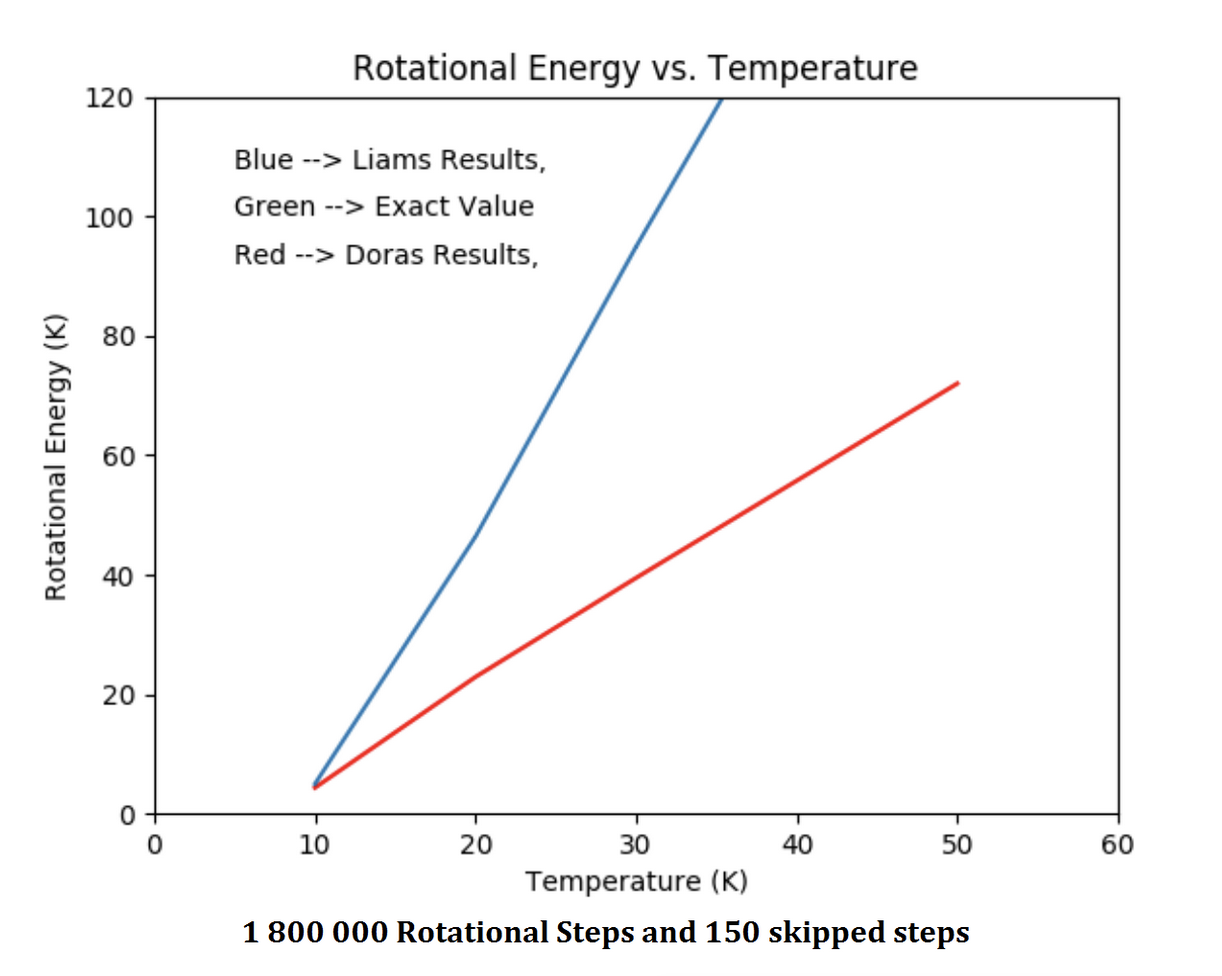
\includegraphics[width=120mm]{BADErotvsT.png}
%    \label{fig:label}
%\end{figure}

The results after the bug fix were as follows;

\begin{center}
\begin{tabular*}{\textwidth}{ | p{0.2\textwidth} | p{0.348\textwidth}| p{0.348\textwidth}|}
\hline
\textbf{Temperature} & \textbf{Erot MoRiBS} (in Kelvin) & \textbf{Erot MMTK} (in Kelvin) \\ 
\hline 
10.0 K & 4.338763 & 4.1465 \\ 
\hline
20.0 K & 22.88446 & 22.638 \\
\hline 
30.0 K & 39.46542 & 39.894 \\ 
\hline 
50.0 K & 71.99282 & 69.544 \\
\hline 
\end{tabular*}
\end{center} 

which generated the plot;

\begin{figure}[!h]
    \centering
    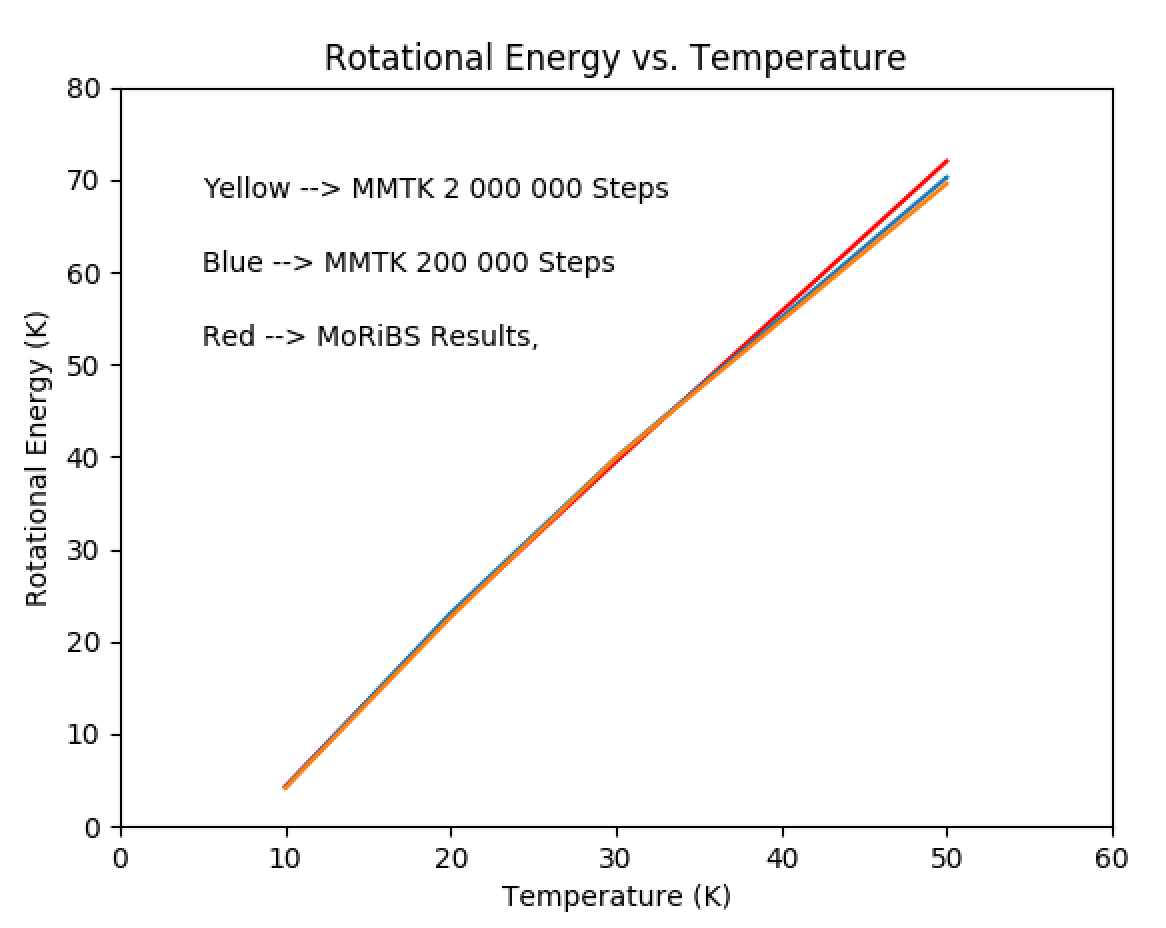
\includegraphics[width=120mm]{GOODErotvsT.png}
    \label{fig:label}
\end{figure}

we can safely move away from the rotation only testing. 

\subsubsubsection{Translation Only}

Our Hamiltonian is as follows;

\begin{equation} \label{eq:3}
\hat{H} \hspace{0.125cm} = \hspace{0.125cm} \hat{T}_{trans} \hspace{0.125cm} ,
\end{equation}

and so our solution should be roughly \begin{math} \frac{3 N k_{B} T}{2} \end{math}. We ran 5 simulations at \begin{math} T = \Big( 10 , 20 , 30 , 50 , 100 \Big) \end{math}, each with just 1 molecule (\begin{math} N = 1 \end{math}). These are our results.

\begin{center}
\begin{tabular*}{\textwidth}{ | p{0.2\textwidth} | p{0.28\textwidth}| p{0.22\textwidth}| p{0.16\textwidth}|}
\hline
\textbf{Temperature} & \textbf{Expected Solution} & \textbf{Etrans MMTK} & \textbf{Error} \\ 
\hline 
10.0 K & 15.0 K & 15.854 K & 0.0645 K \\ 
\hline
20.0 K & 30.0 K & 29.537 K & 0.1334 K \\
\hline 
30.0 K & 45.0 K & 44.704 K & 0.1990 K \\ 
\hline 
50.0 K & 75.0 K & 74.209 K & 0.3388 K \\
\hline 
100.0 K & 150.0 K & 146.349 K & 0.6692 K \\
\hline 
\end{tabular*}
\end{center} 

Firsly I want to clear up that the error is not meant to represent the difference between the expected solution and the acquired solution. It is simply the standard deviation of the distribution used to obtain \textbf{Etrans MMTK}, which itself is an average value. 

The data seems to agree well with the theoretical prediction. 

\subsubsubsection{Rotation + Potential}

Our Hamiltonian is as follows;

\begin{equation} \label{eq:3}
\hat{H} \hspace{0.125cm} = \hspace{0.125cm} \hat{T}_{rot} + \hat{V}_{pot} \hspace{0.125cm} ,
\end{equation}

now we get into which potential we are using. There are three;

\begin{equation} \label{eq:3}
\hat{V}_{pot} \hspace{0.125cm} = \hspace{0.125cm} \vec{\mu} \cdot \vec{E} \cos(\theta) \hspace{0.125cm} ,
\end{equation}

\begin{equation} \label{eq:3}
\hat{V}_{pot} \hspace{0.125cm} = \hspace{0.125cm} - \frac{\mu_{1} \mu_{2}}{4 \pi \epsilon_{0} r_{1 2}^{3}} \bigg( \vec{e_1} \cdot \vec{e}_{2} - \frac{3(\vec{e}_{1} \cdot \vec{r}_{1 2})( \vec{e}_{2} \cdot \vec{r}_{1 2})}{r_{1 2}^{2}} \bigg) \hspace{0.125cm} ,
\end{equation}

and the most complicated one;

\begin{equation} \label{eq:3}
\hat{V}_{pot} \hspace{0.125cm} = \hspace{0.125cm} \hat{V}_{MBPol}  \hspace{0.125cm} .
\end{equation}

I'm not completely sure about the inner workings of MBPol (Many Body Polarizeable), but I think the system allows for changing of dipole moments for many body problems.

We will use MBPol for the simulations we compare to experimental research papers, but to test our running script we will interchangeably use to other two potentials to ensure our code behaves appropriately. MBPol is easily the most accurate potential but its the hardest to implement and also hard to use. The second potential mentioned refers to dipole-dipole interactions, which was already prepared in MMTK when I started this project. I simply had to adapt it for water. The first potential is the simplest. Its just a electric field interacting with a water molecule. Its so simple in fact it has an exact solution which we can compute using perturbation theory. This is helpful for validating the solution of a script. 

Another way of having confidence in your simulation results is to run the same simulation twice using two different scripts (in this case MoRiBS and MMTK), and if they output the same results you can have confidence. 

We will compare the simulations using the \begin{math} \vec{E}_{field} \end{math} potential first (1000 steps);

\begin{center}
\begin{tabular*}{\textwidth}{ | p{0.2\textwidth} | p{0.348\textwidth}| p{0.348\textwidth}|}
\hline
\textbf{Temperature} & \textbf{Erot + Epot MoRiBS} & \textbf{Erot + Epot MMTK} \\ 
\hline 
10.0 K &  &  \\ 
\hline
20.0 K &  &  \\
\hline 
30.0 K &  &  \\ 
\hline 
50.0 K &  &  \\
\hline 
100.0 K &  &  \\
\hline 
\end{tabular*}
\end{center} 

\subsubsection{MoRiBS}

MoRiBS stands for Molecular Rotation in Bosonic Solvents, and as the name suggests, it simulates molecular rotation in bosonic solvents. A boson follows Bose-Einstein statistics (see section on Bose-Einstein statistics) and has half integer spin which has its own consequences (will go into later if I get involved with Worm Algorithm and SuperFluids). 

% idk why this part doesn't compile but its probably something stupid

%To compile density matrix files in the \textbf{nvm\_prop} folder, create a file named \textbf{generate.sh} and in it type \textbf{#!/bin/bash}  in the very first %line. In the next line (you can space it out so this becomes line 3) type the alias (what you use to run code) then the file you want to run, then the %arguments.

For the \textbf{nvm\_prop} folder, type the following to output 3*181 files;

\textit{for x in \{0..180\}; do sbatch  - - export=ithe=\$x generate.sh;done}

From there, you can compile the 3*181 files into 3 files using the \textit{/compile.x} command.  

\subsubsubsection{random instructions}

Whilst in \textit{Tapas' linear rotor MoRiBS} \texttt{/MoRiBS-PIMC/examples/linear\_pigs directory;} 

if you type; python script\_submission\_analysis\_MoRiBS.py -h;  
it prints out list of instructions for running MoRiBS with certain arguments.

\textit{example argument;}  \texttt{python script\_submission\_analysis\_MoRiBS.py tau submission PIMC HF HF 0.1 -d 1.865 -N 10 -Block 1000 -Pass 200}
\texttt{--ROTMOVE -R 10.05}

\vspace{0.5cm}

To copy files from a server (in this case l2mcgrat@graham.computecanada.ca) to my desktop;

\texttt{scp l2mcgrat@graham.computecanada.ca:/home/l2mcgrat/MBPolPaper2/N2P2.png .}

%%%%%%%%%%%%%%%%%%%%%%%%%%%%%%%%%%%%%%%%%%%%%%%%%%%%%%%%%%%
%%%%%%%%%%%%%%%%%%%%%%%%%%%%%%%%%%%%%%%%%%%%%%%%%%%%%%%%%%%
%%%%%%%%%%%%%%%%%%%%%%%%%%%%%%%%%%%%%%%%%%%%%%%%%%%%%%%%%%%

\section{Things I understand at a High Level, but I don't understand at a Low enough Level}

Just gonna outline here some stuff I don't fully understand.

\subsection{Physics}

\subsubsection{PN Junctions}

A PN Junction is formed when a p-type semiconductor and an n-type semiconductor go from being two separate crystals to one full crystal. I have been told that once the crystals are combined, the p-type impurities (such as Ga, B, 14th column periodic table shit) from the P side diffuse over and increase the concentration of p-type impurities on the N side, and vice versa. This diffusion occurs until the electric field created in (what is called) the depletion region inhibits the diffusion of the impurities. My main question is how does this diffusion in the solid state occur in the first place? It seems to me diffusion in the solid state would occur... but over massive timescales. Is the diffusion coefficient really that large? Or is annealing required like what occurs following ionic bombardment to create the impurities in the first place?

\end{document}